%%
%% This is file `thesis.tex',
%% generated with the docstrip utility.
%%
%% The original source files were:
%%
%% nudtpaper.dtx  (with options: `thesis')
%% 
%% This is a generated file.
%% 
%% Copyright (C) 2015 by Liu Benyuan <liubenyuan@gmail.com>
%% 
%% This file may be distributed and/or modified under the
%% conditions of the LaTeX Project Public License, either version 1.3a
%% of this license or (at your option) any later version.
%% The latest version of this license is in:
%% 
%% http://www.latex-project.org/lppl.txt
%% 
%% and version 1.3a or later is part of all distributions of LaTeX
%% version 2004/10/01 or later.
%% 
%% To produce the documentation run the original source files ending with `.dtx'
%% through LaTeX.
%% 
%% Any Suggestions : LiuBenYuan <liubenyuan@gmail.com>
%% Thanks Xue Ruini <xueruini@gmail.com> for the thuthesis class!
%% Thanks sofoot for the original NUDT paper class!
%% 
%1. 规范硕士导言
% \documentclass[master,ttf]{nudtpaper}
%2. 规范博士导言
% \documentclass[doctor,twoside,ttf]{nudtpaper}
%3. 建议使用OTF字体获得较好的页面显示效果
%   OTF字体从网上获得,各个系统名称统一。
%   如果你下载的是最新的(1201)OTF英文字体,建议修改nudtpaper.cls,使用
%   Times New Roman PS Std
% \documentclass[doctor,twoside,otf]{nudtpaper}
%   另外,新版的论文模板提供了方正字体选项FZ,效果也不错哦
% \documentclass[doctor,twoside,fz]{nudtpaper}
%4. 如果想生成盲评,传递anon即可,仍需修改个人成果部分
% \documentclass[master,otf,anon]{nudtpaper}
%
\documentclass[doctor,otf]{nudtpaper}
\usepackage{mynudt}
\usepackage{graphicx}
\usepackage[linesnumbered,ruled,algo2e]{algorithm2e} % for algorithms block by Weiwei
\usepackage{lmodern}% http://ctan.org/pkg/lm
\usepackage{longtable,lscape}
\usepackage{gensymb}

\classification{TP391.41}
\serialno{0123456}
\confidentiality{公开}
\UDC{}
\title{基于多传感器的无人机自主着舰制导与控制技术研究}
\displaytitle{基于多传感器的无人机自主着舰制导与控制技术研究}
\author{孔维玮}
\zhdate{二〇一六年十二月}
\entitle{}
\enauthor{KONG Weiwei}
\endate{\entoday}
\subject{控制科学与工程}
\ensubject{Control Science and Engineering}
\researchfield{模式识别与智能系统}
\supervisor{沈林成\quad{}教授}
\cosupervisor{\quad{}} % 没有就空\quad{}着
\ensupervisor{Prof. SHEN Lincheng}
\encosupervisor{}
\papertype{工学}
\enpapertype{Engineering}
% 加入makenomenclature命令可用nomencl制作符号列表。

\begin{document}
	\graphicspath{{figures/}}
	% 制作封面,生成目录,插入摘要,插入符号列表 \\
	% 默认符号列表使用denotation.tex,如果要使用nomencl \\
	% 需要注释掉denotation,并取消下面两个命令的注释。 \\
	% cleardoublepage% \\
	% printnomenclature% \\
	\maketitle
	\frontmatter
	\tableofcontents
	\listoftables
	\listoffigures
	
	\midmatter
	%\begin{cabstract}
近年来,随着无人作战系统(Unmanned Combat System,UCS)在伊拉克、阿富汗等几场局部战争的广泛使用,展现了无人作战系统的巨大军事价值。作为无人作战系统中的重要组成,无人机所承担的侦察、监视、通信中继、战场评估、攻击引导等任务也日益增多。为扩大无人机的工作半径,提升作战效能,无人机在舰船上回收的需求更加迫切。虽然无人机在地面起飞、降落或回收已经成为常态,但上述过程中的引导方式主要依赖卫星定位导航系统(Global Navigation Satellite System,GNSS)。在未来“反介入/区域拒止(A2/AD)”的战场环境下,仅仅依赖卫星导航系统无法满足无人机在舰船的降落需求。本文主要针对上述研究背景展开工作,主要完成工作和创新点如下:

(1)提出了一种地基/舰基通用的多传感器无人机回收引导系统。该系统主要有两个独立引导单元组成,每个引导单元配备一个二自由度转台和可见光相机、红外相机等传感器。两个独立引导单元的排布可以根据目标无人机的大小和检测距离进行优化配置。本文针对该系统独立分布在跑道两侧的特点,通过对目标位置解算理论推导、误差分析和实验验证,证明了在无人机降落过程中,使用上述两种引导系统的可行性。

(2)设计并实现无人机降落过程中实时目标跟踪和位置解算算法。针对引导无人机降落过程中,无人机目标尺度快速变化和姿态未知的问题,通过改进基于形态学滤波的图像预处理方法,TLD目标跟踪框架和基于主动轮廓的目标位置修正方法,结合转台运动位置和无人机运动的估计,能够准确解算出无人机在降落过程中相对于舰船的位置信息,满足无人机引导和控制系统的需要。

(3)设计并实现基于非线性模型预测控制(NMPC)和总能量控制(TESC)的无人机着舰控制系统。由于无人机机载设备运算能力的约束,本文设计了内环控制器和外环控制器来实现无人机的自主降落。其中内环控制器主要由PI和PID控制器组成,主要完成对无人机姿态的控制;外环控制器主要由非线性模型预测控制器(NMPC)和总能量控制器(TESC)组成,针对基于Dubins Path生成的降落曲线进行跟踪。

(4)设计并实现无人机舰载着舰系统仿真环境并进行户外实验验证。本文基于机器人操作系统(Robot Operation System,ROS)和Gazebo仿真环境构建了无人机舰载着陆软件在回路仿真系统(SITL)和硬件在回路仿真系统(HIL)。该仿真环境能够满足上述算法的验证需求。通过二自由度转台与多传感器的组合配置,实现在地面机场和水面环境对小型和中型固定翼无人机的引导和自主降落。

上述理论和算法成果分别发表在2012年和2013年的IEEE/RSJ智能机器人与系统国际会议(IROS)会议,得到了领域内同行的认可。基于上述算法的实际飞行测试分别在江西吉安机场和湖南长沙湘江水域进行,验证了基于多传感器的地基引导系统和舰基引导系统的可行性和可靠性。

\end{cabstract}
\ckeywords{无人机;自主着舰;多传感器引导与控制;}

\begin{eabstract}
 In recent years, with the unmanned combat system(UCS) in Iraq, Afghanistan and several other local wars of widespread use, unmanned combat system is showing the great military value. As an important component of unmanned combat system, unmanned aerial vehicles(UAVs) are increasingly assigned with reconnaissance, surveillance, communication relay, battlefield evaluation and attack guidance. In order to expand the operating radius of UAV, improve combat effectiveness, the demand of autonomous landing on a destroyer or carrier is continuing to grow. Although UAVs take off and landing on the standard airport is quite common, navigation in the above maneuvers relies mainly on the Global Navigation Satellite System (GNSS). In the future A2 / AD battlefield environment, the satellite navigation system alone can not meet the UAVs' landing demand. This paper aims at the above research background, the main work and innovation are as follows:
 
(1) A ground / ship-based multi-sensor unmanned aerial vehicle (UAV) recovery and guidance system is proposed. The system consists of two independent guidance units, each with a two degrees of freedom PTU(Pan/Tilt Unit) and visible light camera, infrared camera or other sensors. The configuration of the two independent guidance units can be optimally setup according to the size of the UAV and the proposed detection distance. In this thesis, the feasibility of using the above two guidance systems in the process of UAV landing is proved by the theory of target position solution, error analysis and experimental verification, which is based on the characteristics of the system distributed on both sides of the runway independently.

(2) Design and implement the real-time target tracking and location algorithm in UAV landing process. Aiming at the problem of traking the UAV, size rapidly changing from tiny to large scale, the method of image preprocessing based on morphological filtering, TLD target tracking framework and target position updating based on active contour are improved. During the landing process, the Motion position and unmanned aerial vehicle motion estimation, can accurately calculate the position of UAV relative to the ship's position 

(3) Design and implementation of the non-linear model predictive control (NMPC) and total energy control (TESC) of the UAV landing control system. Due to the computation constraints of UAV on-board equipment, the inner-loop controller and the outer-loop controller are designed to realize the autonomous landing. The inner loop controller is mainly composed of PI controller and PID controller. The outer loop controller mainly consists of nonlinear model predictive controller (NMPC) and total energy controller (TESC) in order to tracking the landing curve which generated by Dubins Path algorithms.

(4) Design and implement the simulation system and experimental verification system for UAV shipboard landing problem. Based on the Robot Operation System (ROS) and Gazebo simulation environment, a software in the loop simulation system (SITL) and hardware in the loop simulation system (HIL) is constructed. The simulation environment can meet the verification requirements of the above algorithms. By selecting PTUs and reltaed sensors, autonomous guidance and landing of the UAV can be achieved at ground and airfields.

The above theoretical and algorithmic results were published in the 2012 IEEE / RSJ Intelligent Robot and Systems International Conference (IROS) meeting in 2012 and were recognized by peers in the field. The actual flight tests based on the above algorithms were carried out in Ji'an Airport of Jiangxi Province and Xiangjiang River of Changsha, Hunan Province, respectively. The feasibility and reliability of the foundation guidance system and ship-based guidance system based on multi-sensor were verified.
 
 
\end{eabstract}
\ekeywords{UAV; Autonomous Landing; Multi-sensor Guidance and Control}

  摘要
	%\chapter*{符号使用说明}
% 可以根据需要在chapter后加星星/去掉星星

\begin{denotation}

\item[HPC] 高性能计算 (High Performance Computing)
\item[cluster] 集群
\item[Itanium] 安腾
\item[SMP] 对称多处理
\item[API] 应用程序编程接口
\item[PI]	聚酰亚胺
\item[MPI]	聚酰亚胺模型化合物,N-苯基邻苯酰亚胺
\item[PBI]	聚苯并咪唑
\item[MPBI]	聚苯并咪唑模型化合物,N-苯基苯并咪唑
\item[PY]	聚吡咙
\item[PMDA-BDA]	均苯四酸二酐与联苯四胺合成的聚吡咙薄膜
\item[$\Delta G$]  	活化自由能~(Activation Free Energy)
\item [$\chi$] 传输系数~(Transmission Coefficient)
\item[$E$] 能量
\item[$m$] 质量
\item[$c$] 光速
\item[$P$] 概率
\item[$T$] 时间
\item[$v$] 速度

\end{denotation}
  贡献
	
	%书写正文,可以根据需要增添章节; 正文还包括致谢,参考文献与成果
	\mainmatter
 	\chapter{绪论}


\section{研究背景和意义}
无人机(UAV, Unmanned Aerial Vehicles)在最近十年中已经成为科技领域最吸引眼球的“关键词”。由于无人机自身具有成本低、机动性好、隐蔽能力强等特点,许多国家开展了基于无人机平台的各类研究。回顾历史,自1918年3月6日第一架现代无人机的出现距今已经近百年的历史,但在现实生活中,由于其安全性、可靠性等原因,无人机离我们的生活仍存在着一定的距离。特别是无人机在户外应用过程中,引导信息主要通过将卫星定位导航系统(Global Navigation Satellite System,GNSS)与惯性导航信息相互融合得到。因此,在GNSS信号较弱或者发生中断的情况下,每年在世界各地均发生多起无人机坠毁事件,带来了巨大的人员和经济损失的同时,也限制了无人机的快速应用和发展。

在这些事故中,无人机操作员的失误导致的事故率高达60\%\cite{arrabito2010human}。在2004年的一份报告中指出\cite{williams2004summary},无人机的起飞和降落阶段过程中,人为因素的影响接近50\%。因此,研究精确可靠、自动化程度较高的着陆系统对无人机装备的战斗力生成至关重要,同时也是无人机通用技术发展的关键环节。下面针对自主起降技术的民用需求和军用需求展开说明。

\subsection{无人机引导回收的民用需求}
近年来,随着我国经济的快速发展和人民生活收入水平的提高,越来越多的人选用民航作为出行手段,因此带来航班密度的显著增加。与此同时,气候原因与空气污染的综合作用导致航班晚点情况愈发严重。为研究气候原因导致飞机无法正常降落的情况,有文章\cite{BigDataLanding}通过分析2012年到2014年春运期间的民航数据(CADA, Civil Aviation Data Analysis)得出:影响航班准点率的雾、雪、霾天气所占比例为28.09\%;在千万级级别机场中,霾影响最严重的是郑州机场,占比例为29.21\%,其次是西安机场,所占比例为26.05\%;而在受雾影响的机场中,长沙机场占39.74\%,武汉机场占32.41\%,西安机场占32.07 \%。由此可见,在航班密度最大的春运期间,航班受天气影响导致延误的比例很大。

与人们直观的认知不同,航班是否能够安全降落,除飞机自身性能外,主要取决于目标机场的可见度情况,根据国际民航通用准则,飞机降落标准由低至高主要分为三类:CAT I类,其决断高度(DH, Decision Height)为$60\ m$、跑道视距(RVR, Runway Visual Range)为$550\ m$;CAT II类,DH为$30\ m$、RVR为$300\ m$;CAT III类,其DH和RVR均为$0\ m$要求,即为真正意义上的盲降。目前,国内除北京、浦东、成都、西安为II类机场外,多数机场为I类,而国内大多数航空公司只能执行I类标准,如果天气条件低于I类,航班就无法降落,只能选择备降或返航,影响航班正点率。因此,如果能够通过辅助设备,提高和拓展飞行员的可见度,则可以显著降低因为能见度原因导致的航班延误,从而提高民航的准点率。

在民用无人机领域,大量的无人机的回收依赖GNSS导航信息,加之没有配套的地面或舰载辅助引导设备,无人机的广泛应用受到了较大限制。

\subsection{无人机引导回收的军事需求}
在军事领域,飞行器的自主起降需求则更为迫切。在有人机方面,随着2012年11月23日,歼-15战斗机首次在航母上成功实施阻拦着舰和滑跃起飞(如图\ref{fig:22_J15Landing_Big}所示),航母舰载机的引导降落问题再次引起世人关注。一般而言,为了保证舰载机正确返航和着舰,现代航母均配备有战术空中导航系统、空中交通管制系统和着舰引导系统。完整的着舰过程实质上是一场接力导航:当距离航母300公里时,归航舰载机由战术空中导航系统指挥引导;距离100公里时,由空管雷达接手;距离30公里时,再次由战术空中导航系统引导;距离10公里时,自动着舰系统开始引导;距离3公里时,进入舰上光学助降系统工作区域,最后据此着舰。

\begin{figure}[htb]
	\centering%
	\subfloat[X-47B着舰钩索的瞬间]{%
		\label{fig:01_X47B_Landing}
		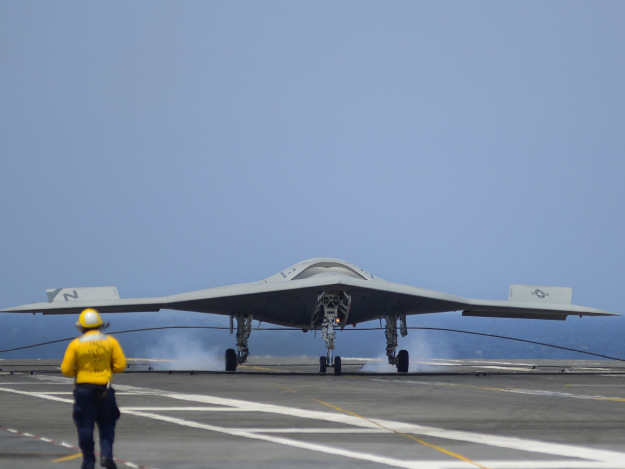
\includegraphics[height=5cm]{Figs/01_X47B_Landing.jpg}}\hspace{0.7em}%
	\subfloat[歼15着舰钩索的瞬间]{%
		\label{fig:22_J15Landing_Big}
		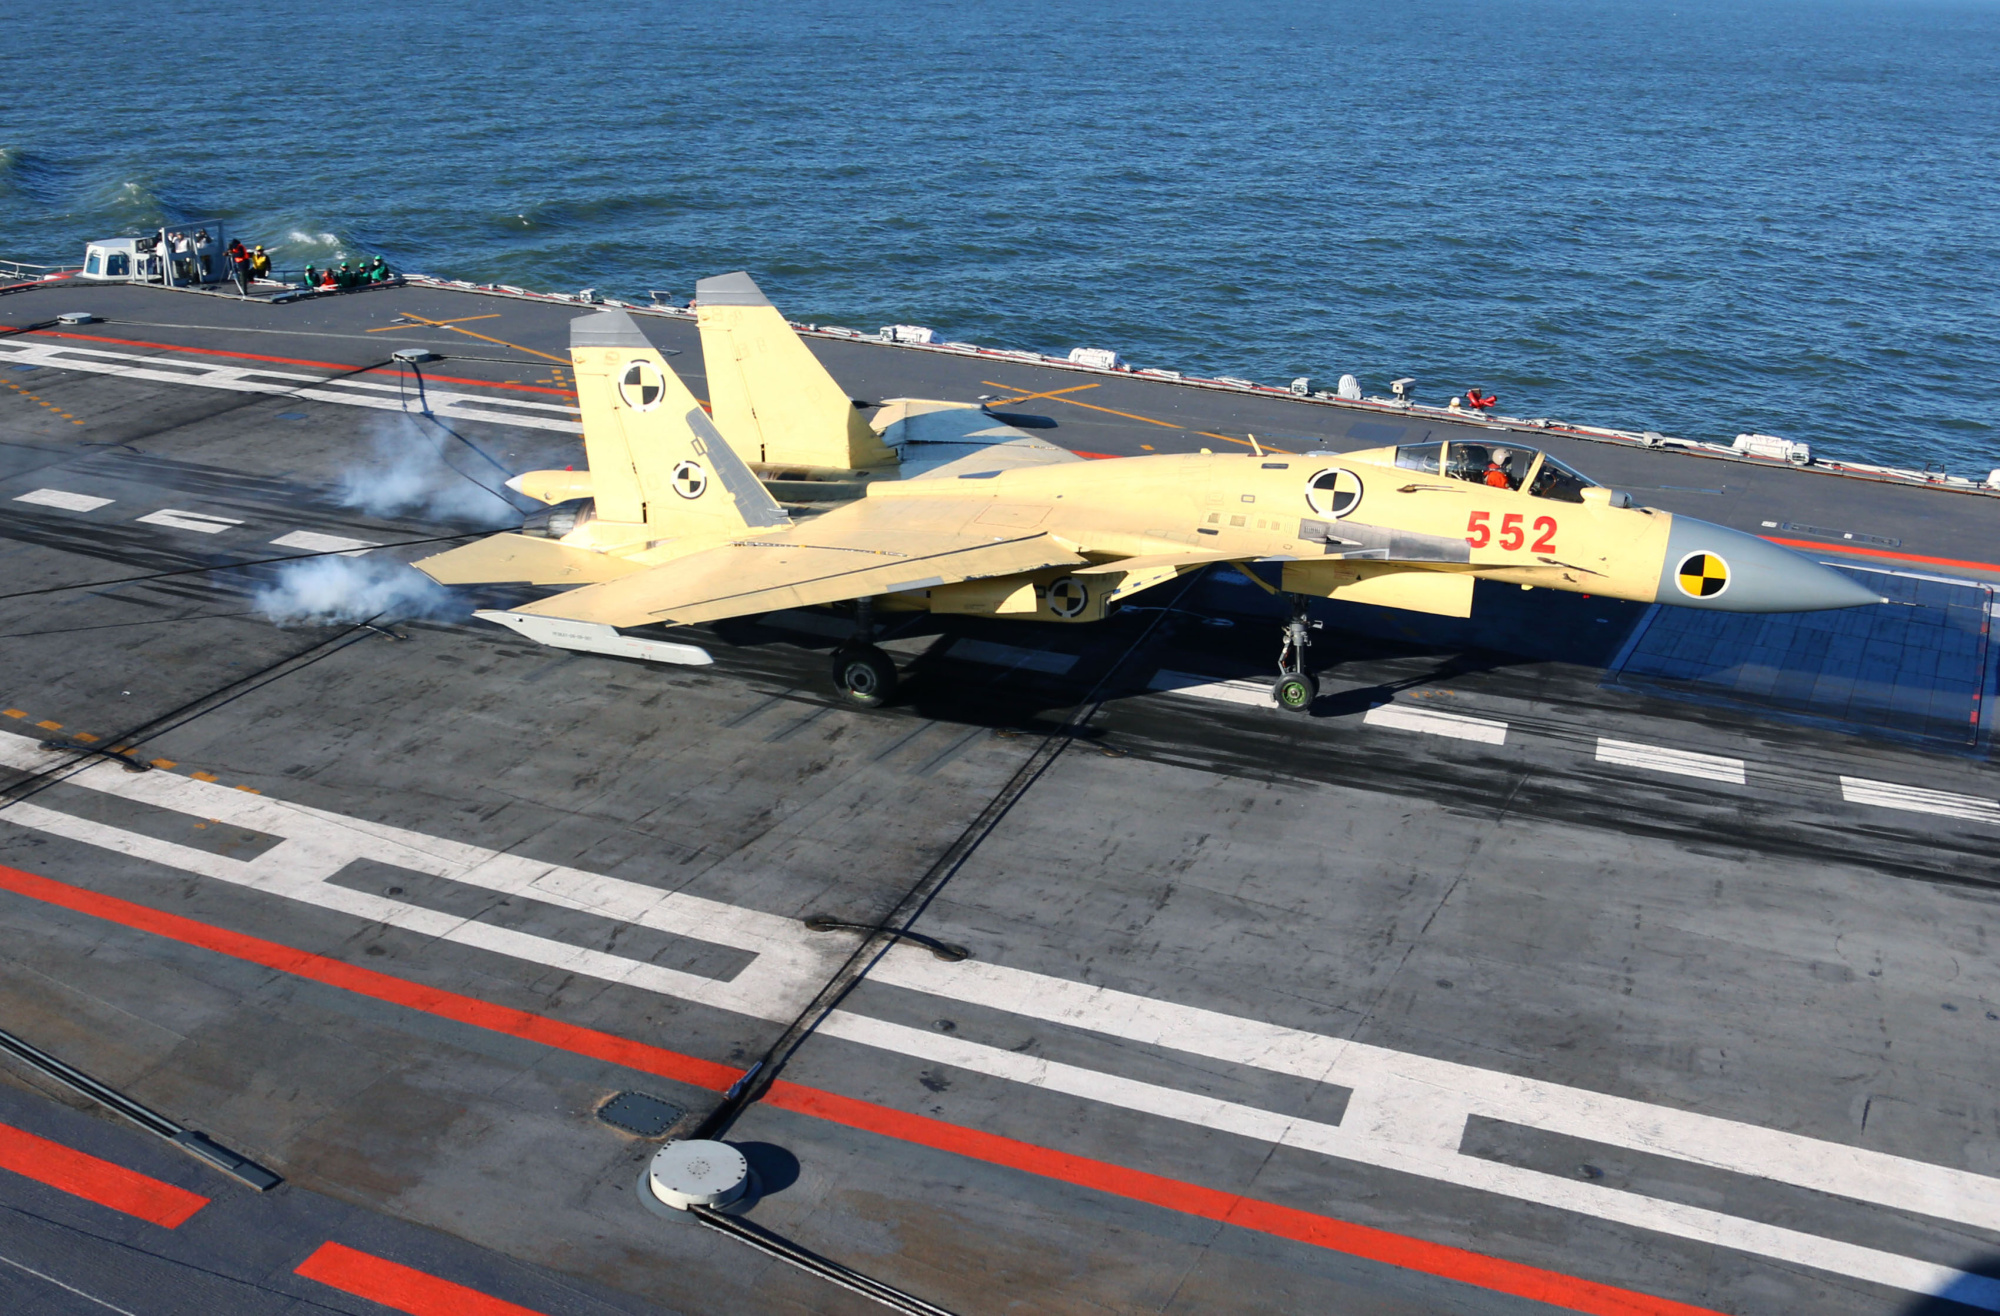
\includegraphics[height=5cm]{Figs/22_J15Landing_Big.jpg}}
	\caption{中美海军飞行器着舰瞬间}
	\label{fig:01_Landing}
\end{figure}

在舰载机降落过程中,飞行员除利用光学助降系统提供的信息进行修正外,航母舰舰载机着陆通常还依赖于人工辅助降落信息。在美航母上,通常由6人组成的着舰信号官(Landing Signal Officer,LSO)位于航母着舰区后部左舷,依靠视频监视系统所拍摄的实时图像及相应参数,通过无线电及灯光等多种手段对舰载机飞行员发出相应着舰指令(如图\ref{fig:20_LSO_USA}所示)。这6人分工和人员配置:(1)担当舰载机着舰引导操作的LSO;(2)利用飞行员助降视频(HUD)显控台引导飞机进场着舰顺序的助理LSO;(3)记录着舰成绩/等级的见习LSO;(4)担任舰内联络的下士联络员;(5)舰载机着舰前尾钩、起落架、襟翼状态的观察员;(6)负责监察着舰引导小组工作的负责人。而在公开的资料中,我国的有人机着舰也采用了类似LSO的人工辅助引导手段,其工作状态如图\ref{fig:21_LSO_China}所示。

\begin{figure}[htb]
	\centering%
	\subfloat[我国“辽宁号”航母上的LSO]{%
		\label{fig:21_LSO_China}
		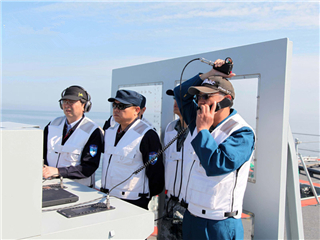
\includegraphics[height=4cm]{Figs/21_LSO_China.jpg}}\hspace{4em}%
	\subfloat[美军航母上的LSO]{%
		\label{fig:20_LSO_USA}
		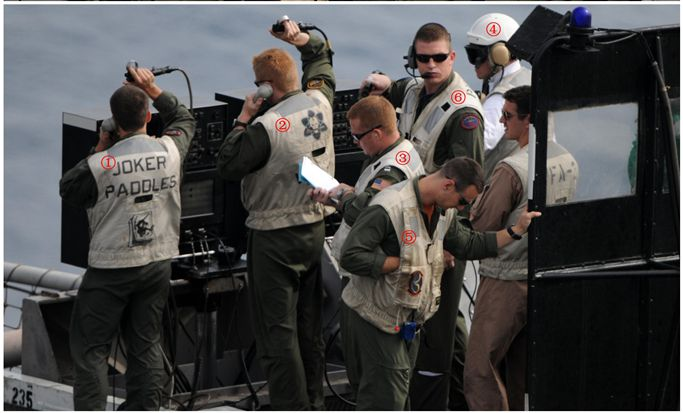
\includegraphics[height=4cm]{Figs/20_LSO_USA.jpg}}
	\caption{中美两国海军LSO工作图}
	\label{fig:21_LSO}
\end{figure}

无人机方面,在降落阶段无人机往往变成了“有人机”,一般会有多个人员进行操控和监视,以免出现差错。所以,本来希望减少人员工作负担的无人机,在降落阶段却往往成为让人担心的“微型炸弹”。为解决无人机的自主起降问题,早在2007年,美国诺斯鲁普·格鲁曼公司开始基于X-47B无人机和美国海军“无人作战航空系统-验证机”(UCAS-D)项目,开发和验证一种自主起飞/拦阻着舰型无人作战飞机。项目合同规定,诺格公司需要研制两架X-47B验证机,完成在航母上自主起降能力的验证,并在完成与航母一体化验证试验后,验证空中自主加油能力。如图\ref{fig:14_LandingAreaX47B2}所示,美国为开展相关研究,在Patuxent River试验基地展开岸基测试,并绘制了模拟甲板起降范围的模拟跑道(如图\ref{fig:10_LandingAreaX47B1}黄色箭头所示),这些细节体现了美国军方对这项技术的重视程度。
\begin{figure}[htb]
	\centering%
	\subfloat[位于海岸边的美军Patuxent River试验基地卫星图片]{%
		\label{fig:14_LandingAreaX47B2}
		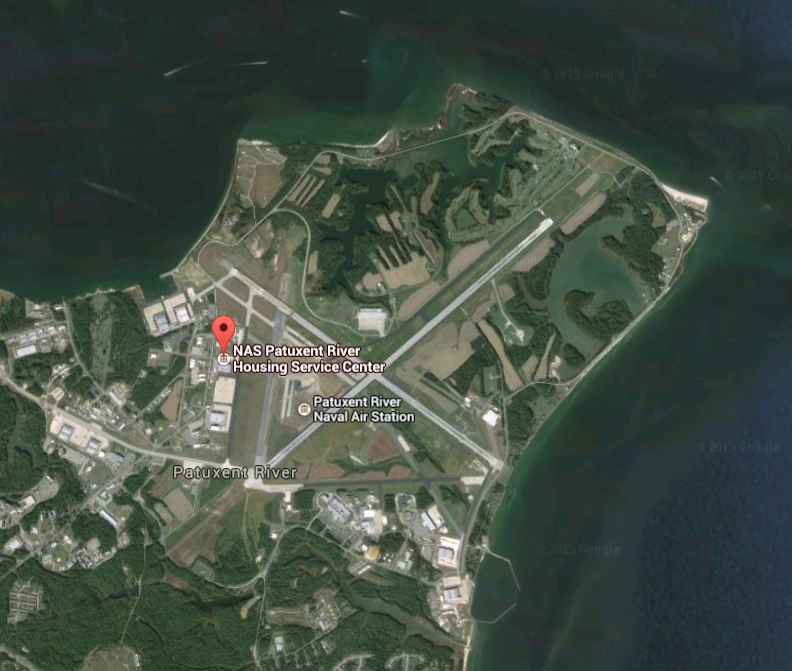
\includegraphics[height=6cm]{Figs/14_LandingAreaX47B2.jpg}}\hspace{0.7em}%
	\subfloat[黄色箭头所指为模拟航母甲板区域的专用跑道]{%
		\label{fig:10_LandingAreaX47B1}
		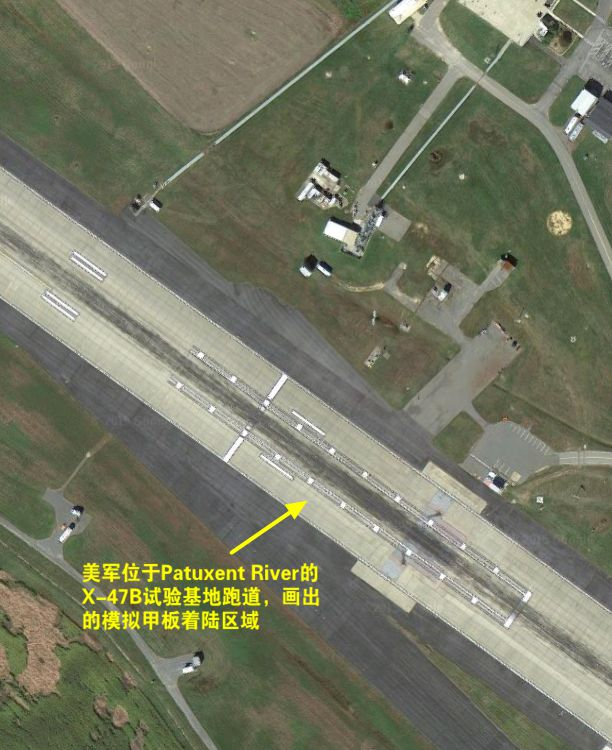
\includegraphics[height=6cm]{Figs/10_LandingAreaX47B1_1.jpg}}
	\caption{美军Patuxent River试验基地}
	\label{fig:14_LandingAreaX47B}
\end{figure}

在沉寂消息多年后,2013年7月,X-47B完成举世瞩目的首次航母自主降落,如图\ref{fig:01_X47B_Landing}所示)。根据公开资料显示\cite{X_47B},X-47B总共完成37次接触甲板测试(Deck Touchdown Test)和30次复飞(Touch-and-go)测试。在2014年3月,由于X-47B及其配套系统完成了人类历史上首次无人飞行器在航空母舰的全自主测试,“X-47B技术团队”获得美国航空协会最重要的“罗伯特·科利尔奖(Robert J. Collier Trophy)”\cite{X_47B_Award}。值得关注的是,该奖项曾经颁奖给诸多美国军用项目,如“全球鹰”无人机系统、“大黄蜂”战机系统、B2轰炸机系统等,由此可见X-47B及其配套系统在理论和工程上所具有的重要意义。此外,在各类报道中也特别提到:该系统精确的导航系统满足了飞行器降落在运动中的航母甲板上,具有里程碑意义\cite{X_47B_Report}。2014年8月,X47-B开展进一步测试,在完成与F/A-18F联合飞行验证后,在90秒内完成自主着舰、折叠机翼、撤出着舰区等一些列动作。其中,4次拦阻着陆,9次复飞再着陆。由于其优秀的控制性能,同月,美国海军计划利用X-47B开展空中自主加油的验证。根据公开资料判断,X-47B的降落除机载传感器外,舰载的JPALS或类似的雷达系统应当提供了辅助信息,如图\ref{fig:X47B_LandingOptical}所示。

\begin{figure}[htb]
	\centering%
	\subfloat[X-47B公布的视频中,跑道一侧的疑似毫米波雷达引导系统]{%
		\label{fig:09_X47BwithRadarGround}
		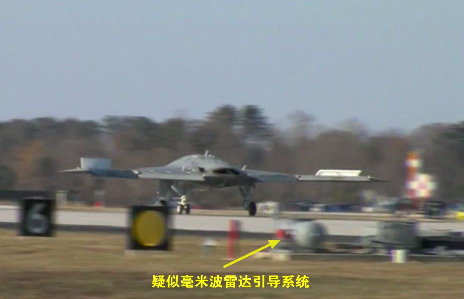
\includegraphics[height=5.2cm]{Figs/09_X47BwithRadarGround.pdf}}\hspace{1em}%
	\subfloat[X-47B公布的视频中,位于舰岛的疑似毫米波雷达引导系统]{%
		\label{fig:02_X47B_LanidngwithRadar1}
		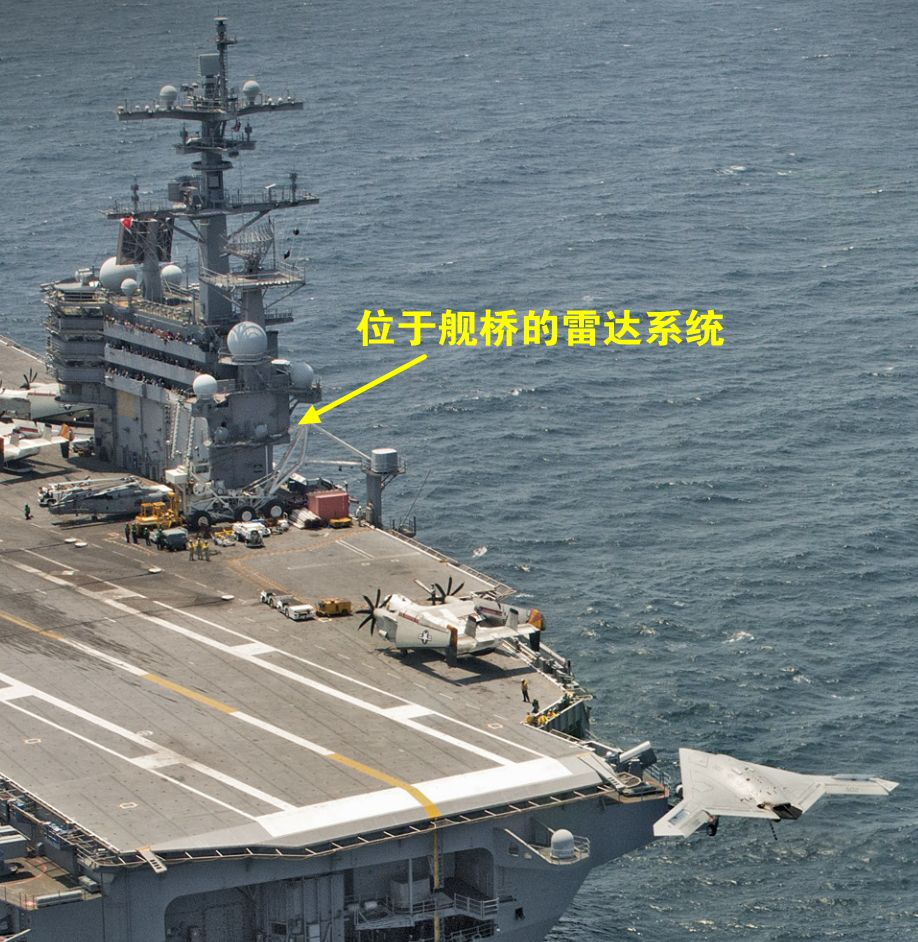
\includegraphics[height=5.2cm]{Figs/02_X47B_LanidngwithRadar1.jpg}}
	\caption{X-47B疑似使用的引导系统}
	\label{fig:X47B_LandingOptical}
\end{figure}



除X-47B这一机型之外,在2014年出版的《2030年的武器装备》\cite{2030equipment}一书中提到,作为美军太空机动飞行器的验证机型X-37B轨道飞行器(OTV, Orbital Test Vehicle),其在返回过程中,运用航空器的导航与指导技术,采用惯性导航和GPS的组合式导航方式,在接近跑道前,以20°的下滑角,350 km/h的速度进场,其降落过程和姿态与X-47B相似(如图\ref{fig:31_X37B_Landing}所示)。根据公开资料显示,X-37B的自主再入和着陆系统采用了惯性导航和GPS的组合式导航。截至到2014年10月17日,X-37B已经完成三次飞行试验,其再入与着陆技术得到波音公司和美国军方的认可。此外,根据2015年2月23日的公开报道,X-37B轨道测试飞行器团队(X-37B Orbital Test Vehicle Team)荣获2015年美国AIAA颁发的年度最高奖项——杰出贡献奖(Award for Excellent)\cite{X_37B}。在颁奖的公告中特别提到,自主降落技术是X-37B的关键技术之一。

\begin{figure}[htb]
	\centering%
	\subfloat[X-37B降落沿跑道方向正视图]{%
		\label{fig:31_X37B_Landing1}
		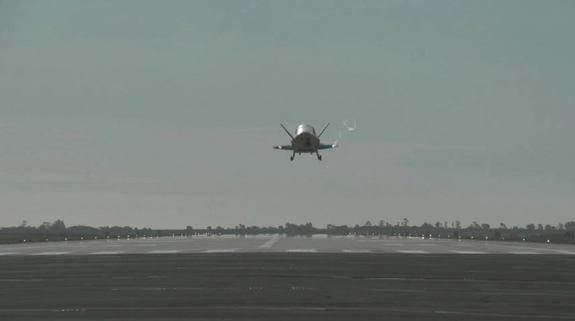
\includegraphics[height=4cm]{Figs/31_X37B_Landing1.jpg}}\hspace{0.7em}%
	\subfloat[X-37B降落侧视图]{%
		\label{fig:32_X37B_Landing2}
		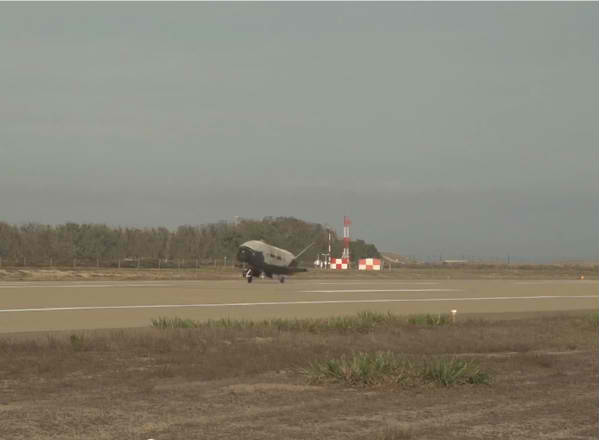
\includegraphics[height=4cm]{Figs/32_X37B_Landing2.jpg}}
	\caption{X-37B完成自主降落}
	\label{fig:31_X37B_Landing}
\end{figure}

综上所述,无人机自主起降技术,特别是舰载无人机自主起降技术是无人机广泛使用的基础和关键。能够在舰载环境,完成无人机的自主回收工作,具有很大的现实意义。


\section{军事和工业领域的引导降落系统}
\subsection{普通飞行器引导降落系统}
\subsubsection{仪表着陆系统}
在航空业发展初期,仪表着陆系统(ILS, Instrument Landing System)作为飞行器的主要着陆手段。该系统于1919年通过美国国家标准局的试验,并在二次大战期间得到广泛应用。1949年,国际民航组织规定仪表着陆系统作为着陆系统的国际标准。该系统主要由地面站和机载设备组成,主要通过机载接收机解算由地面航向信标和下滑信标独立产生的水平和交叉方向波束(波束频率不同),得到飞机的位置信息,即方位角、仰角和距离。该系统的示意图如图\ref{fig:07_ILS}所示。同时,民航组织根据需要,对不同气象条件下的进场标注进行了明确规定。其中,CAT I级别的高度主要通过气压计进行判读,CAT II和CAT III主要通过雷达高度计(Radio Altimeter)进行判读,不同级别的决断高度是飞行员做出是否复飞的基本准则。该系统的优点是具备较好的引导能力,可以为飞行员提供有效方位信息。但在当前电磁频谱环境复杂的机场附近,往往难以得到理想的引导控制精度,因此不能满足无人机系统的降落需求。该系统示意图如\ref{fig:07_ILS}所示。

\begin{figure}[htb]
	\centering%
	\subfloat[飞机在右偏,高度高于标准下滑曲线时的机载仪表显示]{%
		\label{fig:07_ILS1}
		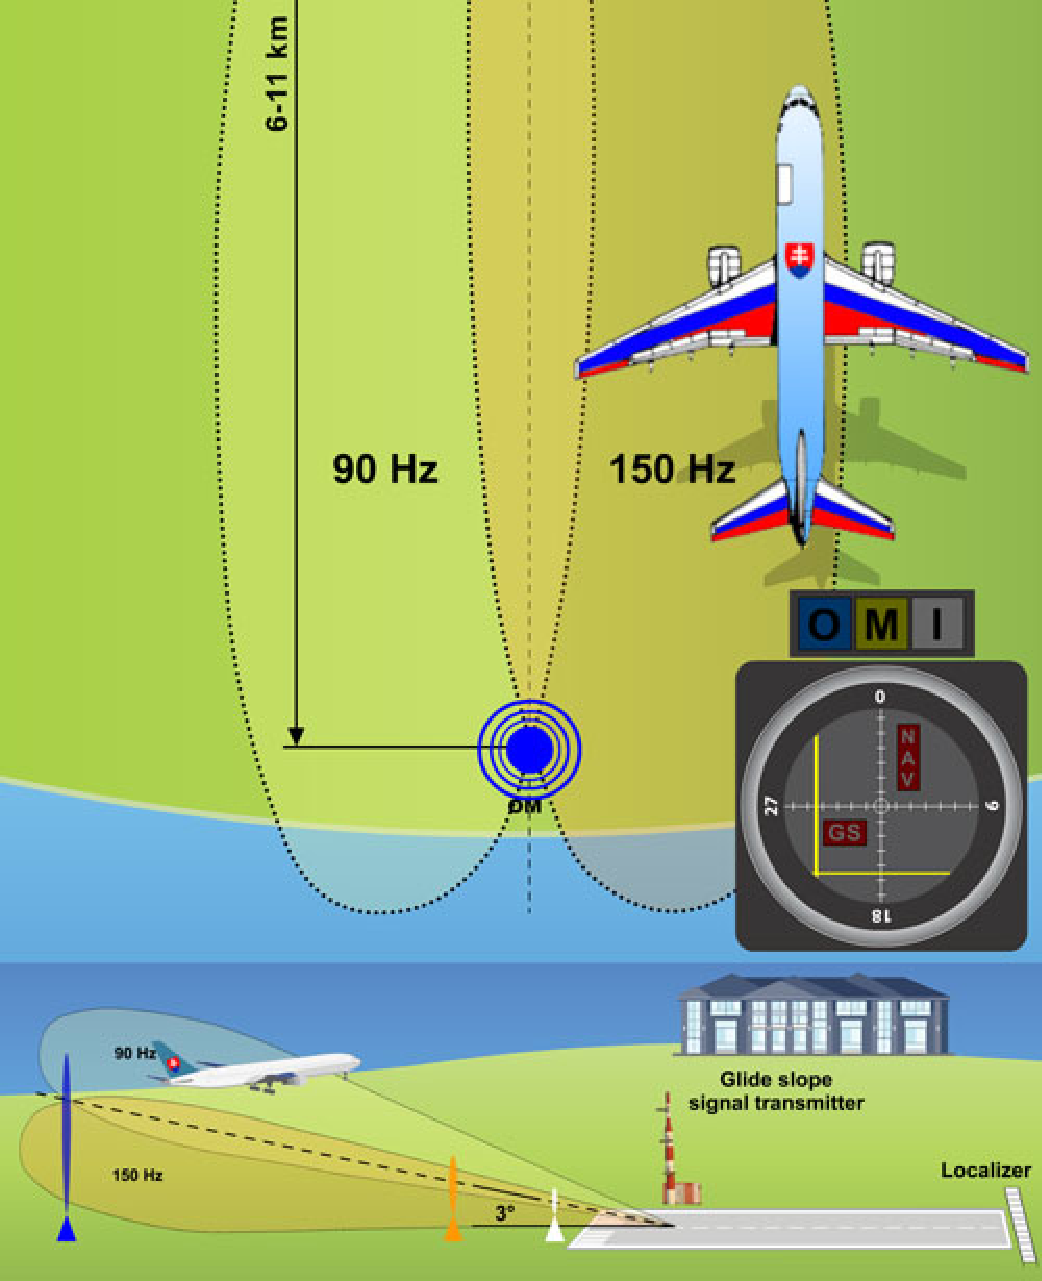
\includegraphics[height=7cm]{Figs/07_ILS1.pdf}}\hspace{4em}%
	\subfloat[飞机在左偏,高度低于标准下滑曲线时的机载仪表显示]{%
		\label{fig:08_ILS2}
		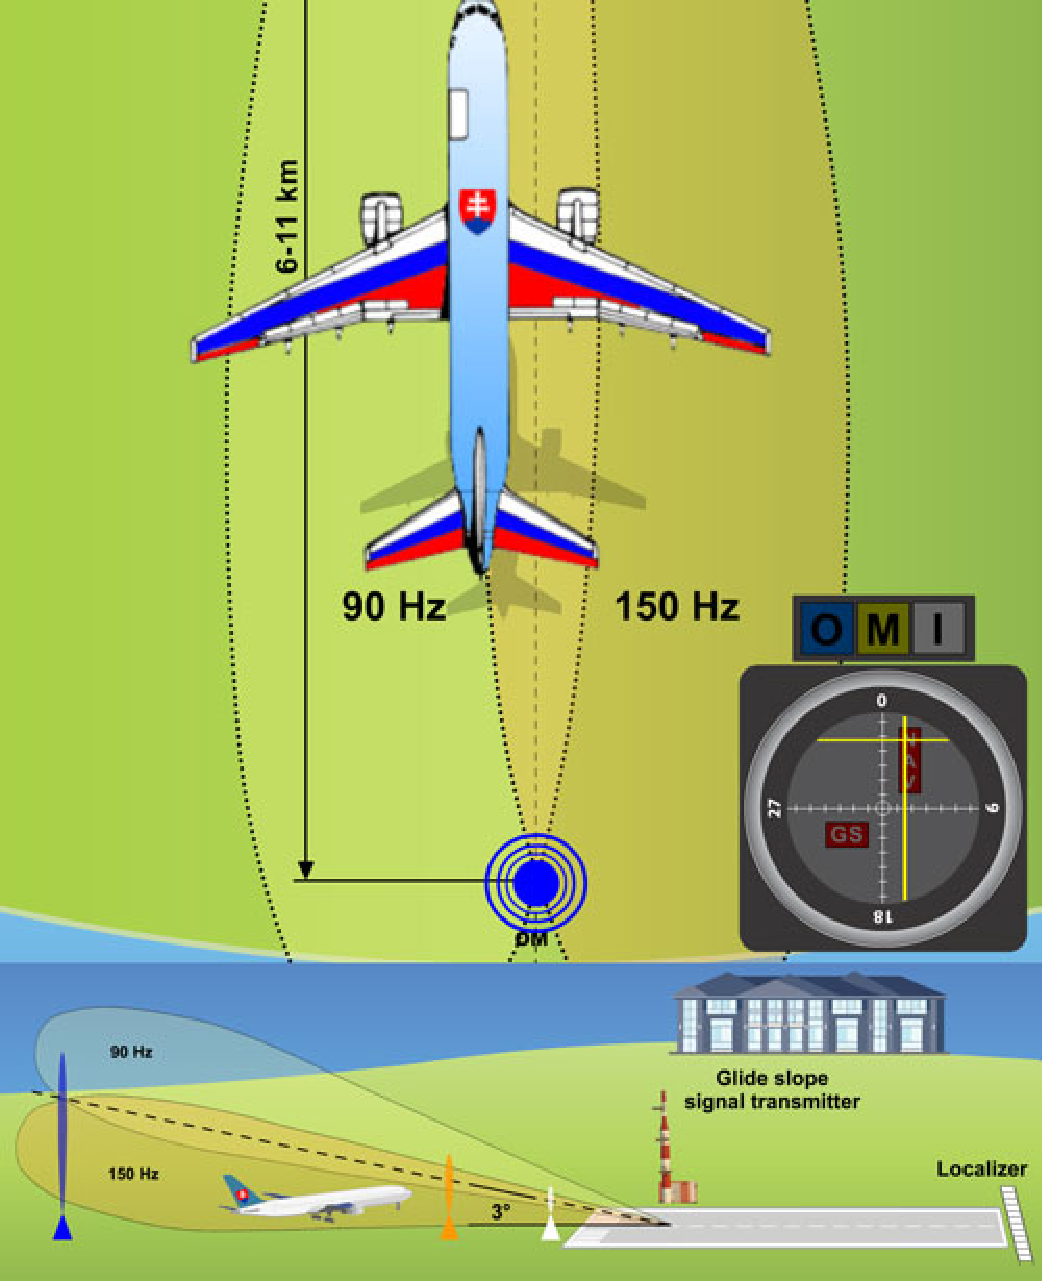
\includegraphics[height=7cm]{Figs/08_ILS2.pdf}}
	\caption{仪表着陆系统示意图}
	\label{fig:07_ILS}
\end{figure}

\subsubsection{雷达着陆系统}
随着二次大战对雷达在军事领域的广泛使用,美军在1943年研制了首套雷达着陆系统(GCA,Ground Control Approach),并于1946年拓展到民用领域。该系统通过地面引导雷达提供精确的位置信息,地面领航员根据雷达显示的下滑路径偏差与飞行员通话,进而操作飞机完成降落。随着技术发展,在雷达系统计算出下滑偏差后,可以根据飞机类型进行引导率计算,形成控制指令后反馈给飞机,协助飞行员或机载飞行系统完成下滑控制。这种方法也被称为“数据链+雷达”系统,至今仍然作为一种可靠的技术手段在航母和军用机场使用。

\subsubsection{微波着陆系统}
1978年,时间基准波束扫描技术(TRSB, Time Reference Scanning Beam)作为微波着陆技术的国际标准得到ICAO的认可。该系由地面方位台、仰角台、精密测距器和机载接收机组成。方位台和仰角台通过向空中发射扫描信号,机载接收机通过测量两次波束信号的时间间隔,得到飞机在空间的位置。但由于仪表着陆系统的广泛应用以及GNSS导航系统的迅猛发展,微波着陆技术的发展出现了一定的停滞。

\subsubsection{联合精密进近和着陆系统}
随着GPS和DGPS技术在美军的广泛应用,一套联合精密进近和着陆系统(JPALS)于2000年在地基完成测试实验。针对舰船本身和飞机都在运动,JPALS需采用双向的UHF数据链,将舰船测量到自身的GPS的位置,以及其摇摆、俯仰、偏航和向前运动的数据一并传给飞机,与此同时,飞机也将其GPS数据传回舰船。舰载的JPALS并不在意实际的位置误差,仅关注船和飞机偏离的量要相同,其着舰精度满足CAT III级别,纵向和横向精度控制在$1 \m$之内,能够完成航母着舰引导任务。在2005至2006年,JPALS开始替换现有的以雷达为基础的AN/SPN-46舰载精密进场着陆系统。这套系统还可用于舰上的空管,双向的数据链能使舰船以GPS跟踪、标注飞机方向。根据公布的合同要求,系统具备初始能力(IOC)时间为2019年,系统具备完全能力(FOC)时间为2030年。


\subsubsection{OPATS(Object Position and Tracking System)}
OPATS是瑞士RUAG宇航公司在1999年为瑞士空军开发研制的“目标定位跟踪系统”的简称,是一套基于激光技术的无人机自动着陆系统,用于瑞士空军的“巡逻兵”无人机。OPATS系统使用反射回来的激光信号对无人机进行跟踪,对目标无人机的动态位置进行连续测量跟踪,提供无人机在着陆阶段的可靠位置信息,并将高速更新的数据传输到地面站进行处,如图\ref{fig:15_OPTAS}所示。自1999年以来,RUAG已向全球范围内的众多用户交付了超过100套的OPATS系统。该系统的目标检测范围为35米至4000米,精度控制在1.5米。

\begin{figure}[htb]
	\centering%
	\subfloat[OPATS引导降落系统外场配置图]{%
		\label{fig:15_OPTAS1}
		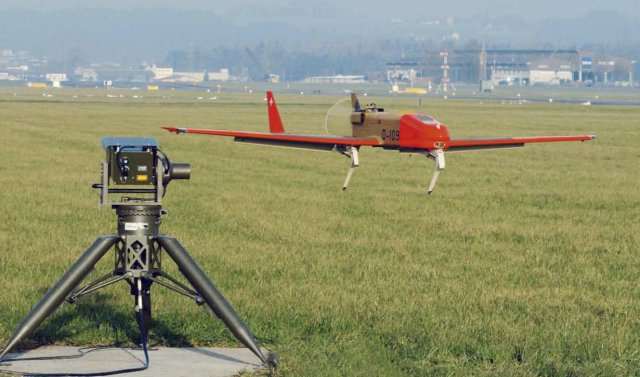
\includegraphics[height=4cm]{Figs/15_OPTAS1.jpg}}\hspace{4em}%
	\subfloat[OPATS引导降落系统框图]{%
		\label{fig:16_OPATS2}
		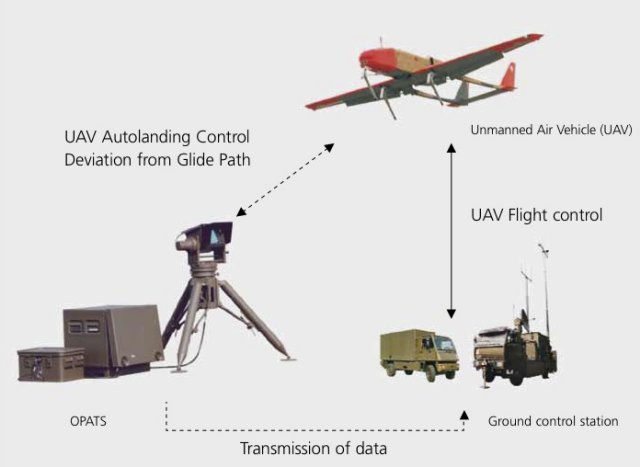
\includegraphics[height=4cm]{Figs/16_OPATS2.jpg}}
	\caption{OPTAS系统介绍}
	\label{fig:15_OPTAS}
\end{figure}


\subsubsection{光学引导系统}
光学助降系统主要依赖于“菲涅尔透镜”(Fresnel Lens)提供给飞行员相应的下滑曲线信息,以便飞行员操作飞机,即该引导系统是人在回路的引导方式。菲涅尔透镜有较好的聚焦性能,在同等焦距上由于传统球面透镜。由助降灯组和稳定平台组成,核心是位于中央的菲涅尔透镜和位于透镜两侧的水平基准灯。	舰载用的菲涅尔透镜系统(FLOLS, Fresenel Lens Optical Landing System)在传统的菲涅尔透镜基础上,将助降灯组与稳定平台结合。稳定平台的惯性系统可以检测舰船运动,使得射出的光束不受航母沉降摇摆的影响。在飞机进行着舰训练时,这套灯光组会释放出黄色、红色和橙色三种不同色彩光的下滑坡面,并以这三种光来界定高低位置。黄色光是高的下滑坡面,红色光是低的下滑坡面,橙色光是正确的下滑坡面。飞行员根据光所标定的位置在橙色光区域内下滑,就可以正确安全地着舰。


\subsubsection{基于UCARS的自主回收}
无人机通用自动回收系统(UAS Common Automatic Recovery System,UCARS)-V2系统(如图\ref{fig:29_UCARS})由内华达山脉公司(SNC)设计,为MQ-8B和MQ-8C火力侦察兵旋翼无人机的自主着陆提供引导控制。该系统是SNC的AN/UPN-51(V)无人机通用自动回收系统(UCARS)的改进型,并根据美军需求,拓展到其他型号的无人机引导降落,例如美国海军陆战队使用的先锋无人机。

该系统的主要传感器是毫米波雷达,该传感器也是军事和工业领域在引导无人机降落过程中使用最多的传感器质之一。毫米波雷达比普通的微波雷达体积更小,同时还具备波束窄和抗干扰能力强的特性;相比于红外传感器,毫米波雷达对于雨雾天气和灰尘的穿透性更强。UCARS系统主要由机载应答系统和舰载跟踪系统组成。跟踪传感器可以检测并计算无人机相对于期望降落点的位置信息,并向无人机提供降落平台的位置和运动状态数据,便于机载系统的导航和控制。目前UVARS系统有V2改进版,该版本使得无人机具备自主降落能力,减少了无人机飞行员的干预。此外,它还具备船舶运动稳定设备,以满足不同海况下的运行需求,该系统的引导控制精度在2.5厘米左右。系统的地基和舰载配置情况如图\ref{fig:29_UCARS}所示。 

\begin{figure}[htb]
	\centering%
	\subfloat[UCARS引导庞巴迪CL-227降落]{%
		\label{fig:29_UCARS1}
		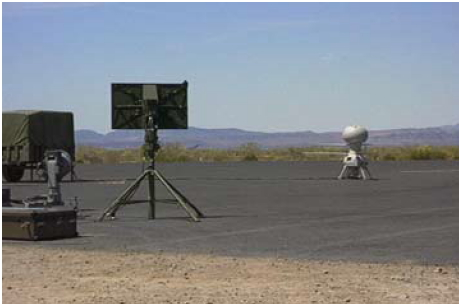
\includegraphics[height=4cm]{Figs/29_UCARS1.jpg}}\hspace{1em}%
	\subfloat[UCARS引导MQ-8B降落]{%
		\label{fig:30_UCARS2}
		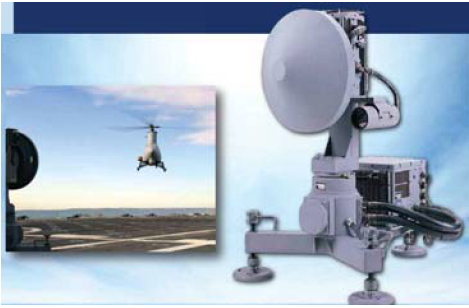
\includegraphics[height=4cm]{Figs/30_UCARS2.jpg}}
	\caption{无人机通用自动回收系统(UCARS)}
	\label{fig:29_UCARS}
\end{figure}

\subsubsection{无人机甲板起降引导系统}
法国DCNS公司开发的无人机直升机甲板起降引导系统(SADA\footnote{此处为法语缩写,Systèmed’Appontage et de Décollage Automatique})\cite{DCNS}使用红外传感器精确跟踪无人机,同时发出飞行指令调整航线直到确保无人机的“鱼叉”式着陆装置对准降落格栅的中心。2008年10,SADA成功将一架奥地利西贝尔公司研制的“坎姆考普特”(Camcopter)S-100无人直升机以自主模式降落在一艘正在地中海航行的法国海军驱逐舰“蒙特卡姆”号(Montcalm)上。该系统的引导控制精度约$30\ cm$。

\begin{figure}[!tb]   
	\centering	
	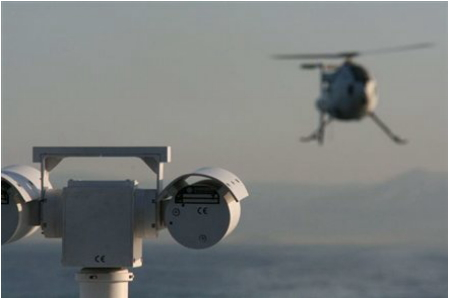
\includegraphics[width=0.5\textwidth]{Figs/24_SADA_Landing.jpg}
	\caption{SADA系统引导无人直升机着舰 }
	\label{fig:24_SADA_Landing}
\end{figure}


\subsubsection{基于D2AD自动甲板起降系统}
2011年,法国DCNS公司和Thales 公司完成无人机直升机在甲板自主降落(D2AD\footnote{此处为法语缩写,Démonstration d'un système d'appontage et d'atterrissage pour drones})的测试。此次海试使用法国海军“拉斐尔”级护卫舰和一架波音H-6U“小鸟”旋翼无人机,实验标志着 D2AD项目为期 4 年的技术验证成果。D2AD系统包括“飞行”部分和“地面”部分,“飞行”部分是无人机的指引标,“地面”部分在飞行甲板使用传感器进行船体运动预报,是无人机的引导站(如图\ref{fig:25_D2AD})。D2AD不依赖于任何卫星定位系统,能够保证垂直起降无人机在舰船上的安全使用。

\begin{figure}[htb]
	\centering%
	\subfloat[D2AD自主甲板降落系统]{%
		\label{fig:25_D2AD_1}
		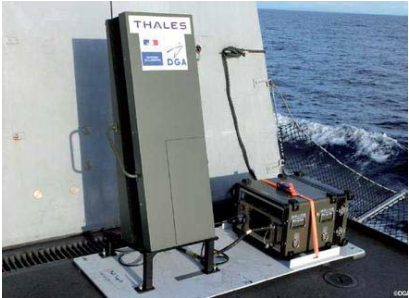
\includegraphics[height=4cm]{Figs/25_D2AD_1.jpg}}\hspace{0.1em}%
	\subfloat[H-6U“小鸟”旋翼无人机]{%
		\label{fig:26_D2AD_2}
		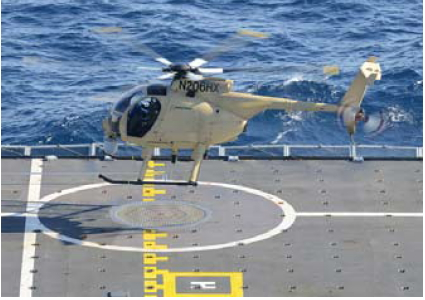
\includegraphics[height=4cm]{Figs/26_D2AD_2.jpg}}\hspace{0.1em}
	\subfloat[机载指引标]{%
		\label{fig:27_D2AD_3}
		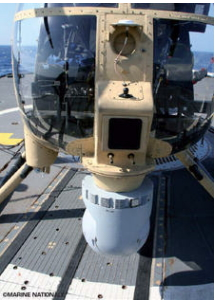
\includegraphics[height=4cm]{Figs/27_D2AD_3.jpg}}
	\caption{D2AD机载引导系统基本构成}
	\label{fig:25_D2AD}
\end{figure}

\subsubsection{基于DeckFinder的降落系统}
2013年6月,奥地利西贝尔电子设备公司的“坎姆考普特”S-100 无人直升机配装欧洲航宇防务集团(EADS)阿斯特里姆公司的“甲板发现者”(DeckFinder)区域定位系统,在一周的时间内完成了一系列旨在演示验证GPS干扰环境中无人机自动起飞与回收能力的飞行试验。“甲板发现者”系统\cite{Deckfinder}包括地面部分和机载部分,其中地面部分包括6台射频发射机,机载部分包括1台接收机。该系统的测距不依赖于GPS,可为航空器提供高精度的三维相对位置信息。根据公布的技术细节,该系统的工作范围约为$1.1\ km$,降落阶段精度优于$20\ cm$,工作频率不低于$15\ Hz$。
\begin{figure}[!tb]   
	\centering	
	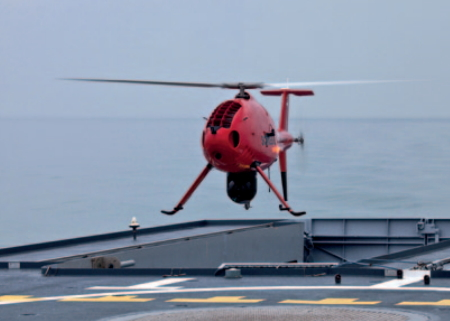
\includegraphics[width=0.5\textwidth]{Figs/28_Deckfinder.jpg}
	\caption{DeckFinder在GPS干扰环境下引导S-100无人机降落}
	\label{fig:28_Deckfinder}
\end{figure}

\subsubsection{基于JPALS的引导降落}
% X-47B
作为固定翼无人作战飞机,X-47B无人机面临着与其他无人机同样的难题:回收过程复杂。根据海军科技网站(Naval Technology)公布的消息\cite{X_47B_UCAS},X47-B的引导控制系统有较强的自主性,其导航系统主要由GPS和视觉系统组成。为提高智能化程度,X47-B还配备了光学系统、红外系统、SAR雷达(SAR, Synthetic Aperture Radar)、地面目标指示器(Ground mMving Tagret Indicator)和海面目标指示器(Maritime Moving Target Indicator)等设备。此外,在自主降落过程中,系统遵循预设的下降曲线对飞机进行引导和控制,操作员只是监视整个下降过程。虽然X-47B使用的具体引导降落方式没有公开,但通过公开视频和图像分析(如图\ref{fig:X47B_LandingOptical}所示),X-47B的自主着舰也应用了类似引导系统。

通过阅读相关资料并分析,该联合精确进场与着舰系统(JPALS)由处理、维修和监测系统,UHF数据链,惯性传感器和GPS传感器等组成,可以实现高可靠性和可用性。JPALS将与AN/TPX-42空中交通管制雷达、AN/SPN-46自动着舰系统、AN/SPN-41着舰辅助雷达、着舰信号官显示系统、改进型菲涅耳透镜光学着舰系统、航空数据管理和控制系统集成。2011年7月,F/A-18D“大黄蜂”战机在“艾森豪威尔”航空母舰上实现无人控制自主降落。

% ----- MQ-8B/C
2006年1月,MQ-8B完成了第一次在两栖登陆舰USS Nashville的舰载着陆,实验海域为Chesapeake Bay。2014年8月27日,MQ-8C“火力侦察兵”无人直升机在文图拉县海军基地完成着舰试验。

\subsection{无人机回收方式概述}
在X-47B无人机成功阻拦降落之前,世界各国在舰载无人机回收方面普遍采用的方法是:伞降回收、撞网回收、打捞回收和钩绳回收等。其中,撞网回收和钩绳回收对无人机回收控制精度提出更高要求,需要无人机自身或舰基系统具有较好的引导和控制能力。

\subsubsection{伞降回收}
伞降回收就是利用降落伞回收无人机。无人机从飞行状态到安全回收,整个过程自动完成,对操作人员要求较低。这种回收方式操作简单,是小型无人机回收的一种重要方式,适合对落点没有特殊要求的回收。采用轮式着陆的无人机也可使用伞降回收作为应急回收方案。采用水上伞降回收时,要考虑到无人机落入水中后对机身和内部设备的影响。

\subsubsection{撞网回收}
使用拦截网系统回收无人机是目前小型无人机较普遍采用的回收方式之一。无人机在降落阶段,通过降低高度和减小速度,撞向由弹性材料编制成的阻拦网。美国RQ-2“先锋”无人机和“银狐”无人机均采用
这类回收方式,如图\ref{fig:34_RQ2_Pioneer_Landing}所示。
\begin{figure}[!tb]   
	\centering	
	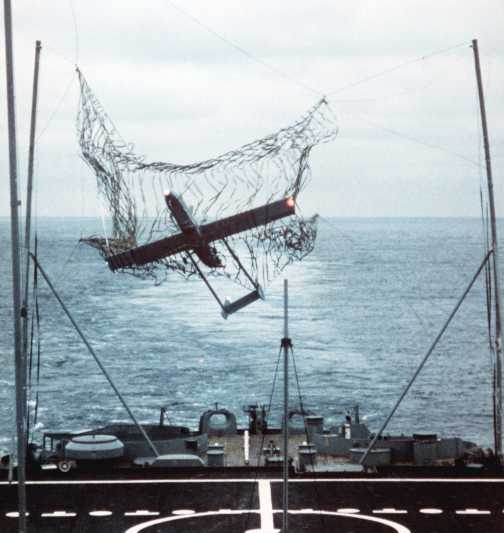
\includegraphics[width=0.4\textwidth]{Figs/34_RQ2_Pioneer_Landing.jpg}
	\caption{RQ-2在舰船完成撞网回收}
	\label{fig:34_RQ2_Pioneer_Landing}
\end{figure}

% Bat UAS
%翼展4.26 m、极长2.0 m、最大起飞重量159 kg、有效载荷34 kg。
%Shadow
%Poineer

\subsubsection{钩绳回收}
该回收方法使用垂直悬浮钢丝的天钩技术。钢丝可以自由的悬浮在吊杆上或者通过风筝把它升起,同时在无人机的翼尖上固定一个自锁的钩子。无人机进场时,径直地飞向钢丝,以便钢丝碰到其中一个机翼的前缘,然后滑向翼尖,通过钩子便可以把无人机锁住。由于航母的摆动幅度通常会限制为横摇2-3度,纵摇1-1.5度,而中小型船只稳定性要差得多,因此必须在横摇13度,纵摇5-6度的恶劣环境下,相比撞网回收,钩绳回收的引导控制需求更高,需要确保无人机在一米大小的回收窗口准确降落。

RQ-21A在2010年称为美国小型战术系统(Small Tactical Unmanned Aircraft System)项目的主力机型,该飞机具备陆基和海基起降能力,能够完成战术侦察、监视、目标指示(Reconnaissance, Surveillance and Target Acquisition,RSTA)功能,其模块化设计可快速替换不同传感器并完成部署。2014年7月,美国海军开始使用RQ-21A系统进行海上综合测试。该型无人机采用钩绳回收方式,如图\ref{fig:33_RQ21_Landing}所示。此外,“扫描鹰”无人机也采用此类方式回收,如图\ref{fig:35_Eagle_Scanner_Landing}所示。

\begin{figure}[htb]
	\centering%
	\subfloat[RQ-21在舰船回收]{%
		\label{fig:33_RQ21_Landing}
		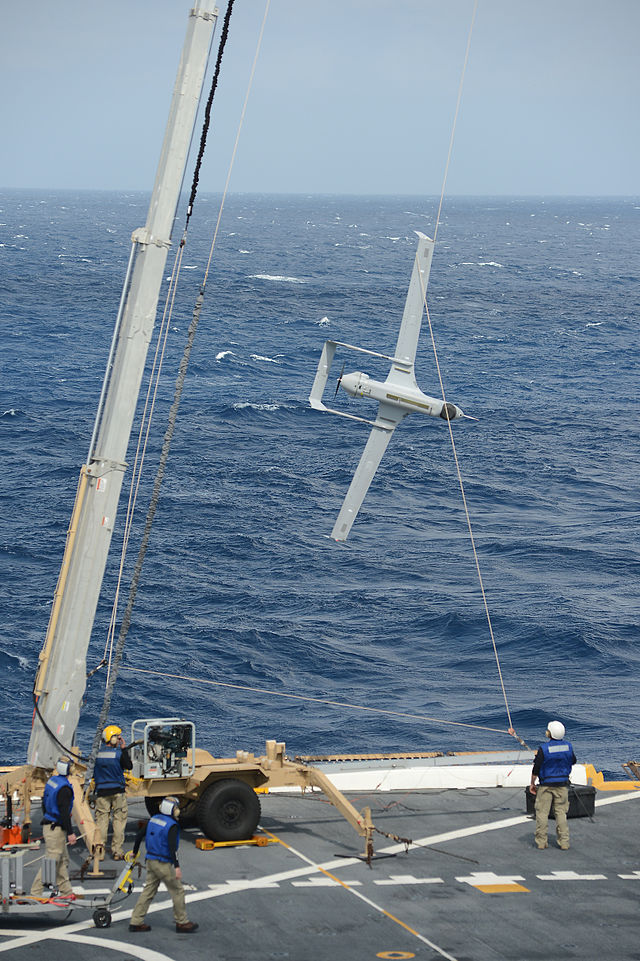
\includegraphics[height=6cm]{Figs/33_RQ21_Landing.jpg}}\hspace{0.1em}%
	\subfloat[“扫描鹰”无人机在舰船回收]{%
		\label{fig:35_Eagle_Scanner_Landing}
		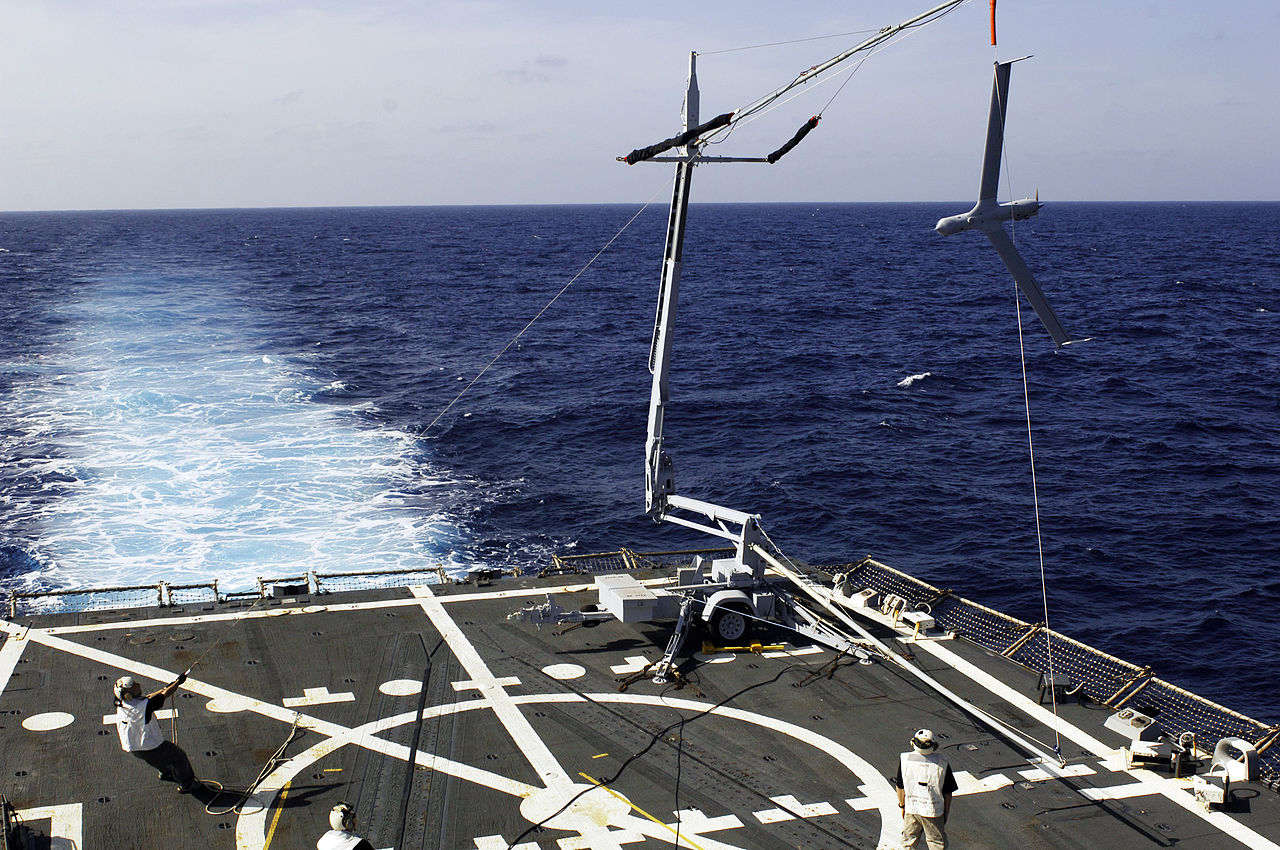
\includegraphics[height=6cm]{Figs/35_Eagle_Scanner_Landing.jpg}}\hspace{0.1em}
	\caption{采用钩绳回收方式的无人机}
	\label{fig:33_RQ21withScanner_Landing}
\end{figure}


\section{学术研究领域的无人机引导降落系统}
由于可见光摄像机成本低廉的特点,基于图像信息的无人机引导和控制在无人机实际应用中扮演十分重要的角色。例如,利用机载摄像机来完成感知规避任务\cite{mejias2010vision}、监视和跟踪任务\cite{campoy2009computer}\cite{mejias2006visual}、自主起飞和降落任务\cite{saripalli2002vision}、实时建图与定位任务(SLAM)\cite{weiss2011monocular}等。此外,通过图像信息对无人机自身位置和姿态进行估计也是今年来的研究重点和热点。比如在空中加油领域、无人机定点区域着陆等。2014年,针对视觉在无人机自主降落领域的研究现状,文章\cite{kong2014vision}系统总结了当前37个世界各地研究单位的工作,总结表格详见附录。本节只针部分内容进行概述。

\subsection{机载传感器引导降落系统} 

早在2003年,Shakernia\cite{shakernia2003vision}的博士论文中提出一种基于视觉的旋翼无人机(Yamaha R-50)的自主降落方案,该方案通过识别放置于六自由度运动平台上的合作标志完成自主降落(如图\ref{fig:chp01_06_shakernia_landing}所示)。其中,通过识别合作标志中的焦点,并使用Linear Two-view Motion Estimation, Non-linear Two-view Motion Estimation和Multi-view Planar Algorithm方法对飞机的位置和姿态进行估计。上述三种方法可以较好的解决特征点共面的飞机和位置姿态估计问题,通过仿真和户外试验,验证了系统的有效性和鲁棒性(位置偏差小于0.05米,角度偏差小于0.5°),但对于非合作目标的识别,不具备求解的通用性。

\begin{figure}[!tb]   
	\centering	
	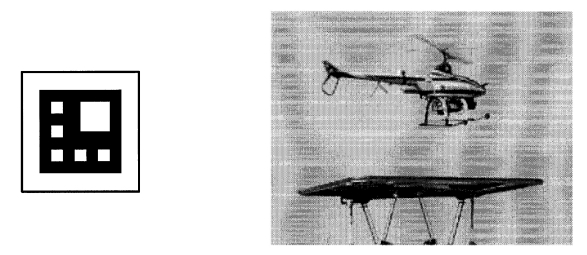
\includegraphics[width=\textwidth]{figs/chp01/chp01_06_shakernia_landing.pdf}
	\caption{基于合作标识的无人直升机自主降落系统}
	\label{fig:chp01_06_shakernia_landing}
\end{figure}


2009年,朱建明\cite{Zhu_Master_2009}对传统“H”形合作目标进行改进将“H”形图标的上端开口封住,改进后的图标能够克服“H”形图标缺乏有方向性的缺点,在地标图案分割的基础上,采用基于灰度变化的角点检测方法,提取合作标志的特征点。

2010年之后,该领域的研究逐渐增多。韩国科学技术院(Korea Advanced Institute of Science and Technology,KAIST)提出一种应用于小型无人机上的视觉引导着陆系统通过视觉引导无人机飞行至安装在地面上的红色圆拱形安全气袋中\cite{huh2010vision},原理如图\ref{fig:chp01_05_korea_landing}所示。
\begin{figure}[!tb]   
	\centering	
	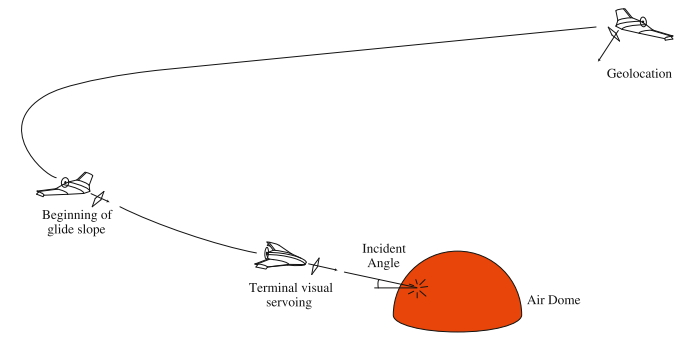
\includegraphics[width=\textwidth]{figs/chp01/chp01_05_korea_landing.pdf}
	\caption{基于红色标志物的无人机回收系统示意图}
	\label{fig:chp01_05_korea_landing}
\end{figure}

李宇\cite{Li_Master_2012}设计了一种由6个圆心已标识出来的红色圆圈组成的合作标志,通过基于仿射不变矩和SVM分类器实现着陆地标的识别,如图\ref{fig:chp01_04_six_circle_landing_pattern}所示。
\begin{figure}[!tb]   
	\centering	
	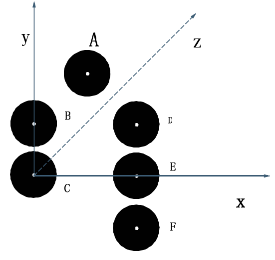
\includegraphics[width=0.4\textwidth]{figs/chp01/chp01_04_six_circle_landing_pattern.pdf}
	\caption{六个圆形合作标识}
	\label{fig:chp01_04_six_circle_landing_pattern}
\end{figure}

H. Jin Kim等人\cite{kim2013fully},针对小型固定翼无人机提出了一种基于机载视觉的撞网回收系统。该系统采用颜色分割和形态学等图像处理算法,通过机载摄像头对无人机回收网进行检测和识别;通过几何位置分析,判断无人机当前的方位信息,设计无人机引导率和控制率;地面控制系统可以向无人机发送控制命令并监测无人机的飞行状态。

德国宇航局在2015至2016年进行了HALE(High Altitude Long Endurance) UAV在运动汽车顶部回收的实验测试,该型号无人机的翼展为$3.3\ m$,最大起飞重量为$21.5\ kg$。该无人机在距离地面车辆$300\ m$左右的距离捕获地面移动车辆,随后地面移动车辆加速至合适的速度,满足无人机的回收需要。在回收过程中,无人机的引导方式主要通过机载摄像机对汽车顶部的合作标识(二维码)进行识别,进而实现相对位置的解算,完成自主降落\cite{Muskardin2016}。由于合作标识的尺寸和机载相机视场角的约束,无人机检测到地面目标点的距离较短,系统有效工作范围较小。
\begin{figure}[htb]
	\centering%
	\subfloat[无人机在回收末状态时,与汽车的速度保持相同]{%
		\label{fig:07_ILS1}
		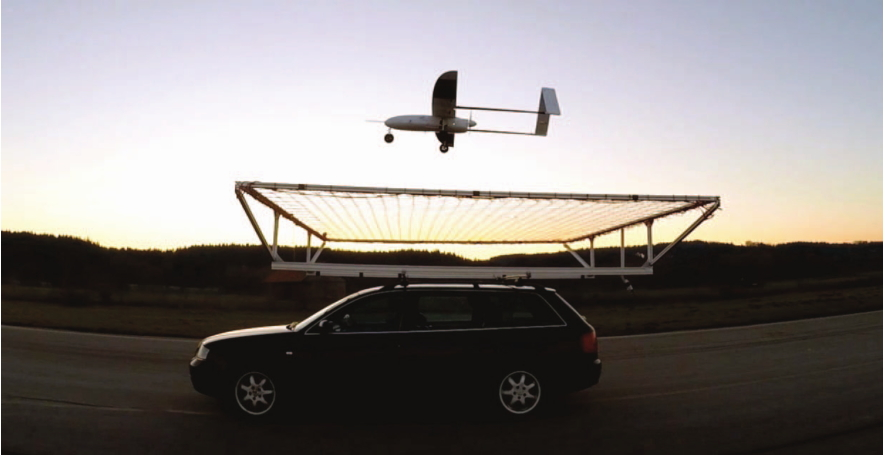
\includegraphics[height=3.5cm]{figs/chp01/chp01_01_DLR_Landing.pdf}}\hspace{0em}%
	\subfloat[机载传感器通过识别车顶的合作标识,实现相对位置的解算]{%
		\label{fig:08_ILS2}
		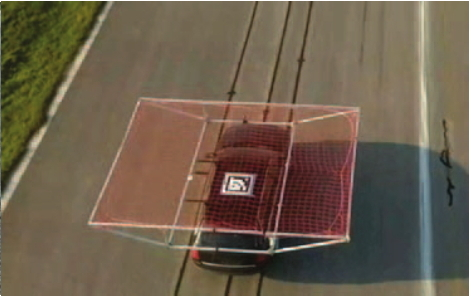
\includegraphics[height=3.5cm]{figs/chp01/chp01_02_DLR_Landing_with_tag.pdf}}
	\caption{德国宇航局车载无人机回收试验图}
	\label{fig:07_ILS}
\end{figure}

2016年5月,卡内基梅隆大学的研究者发布了最新无人直升机降落在海面移动平台\cite{Grocholsky2016}的工作。无人机上装载了长波红外传感器,该传感器适应雨雾天气,最远探测海面移动平台的距离为1.2海里(约2.22公里)。无人机从500米开始,对海面移动平台进行位置估计,并逐渐靠近该平台。在距离195米左右时,机载可见光传感器可以识别位于降落平台的合作标识,并具备对该平台姿态进一步估计的能力,其识别效果如图\ref{fig:chp01_03_CMU_Sea_Landing}所示。在最后50米的距离,激光传感器通过对甲板的三维空间扫描,实现厘米级的位置解算精度。

\begin{figure}[htb]   
	\centering
	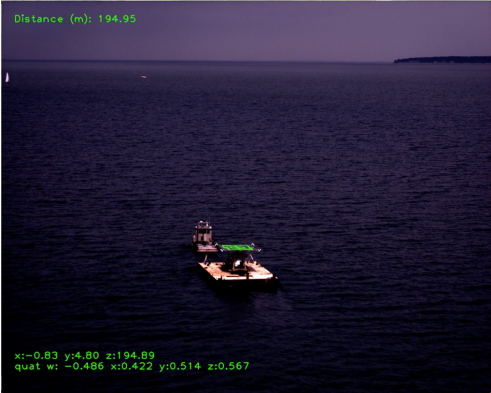
\includegraphics[width=0.6\textwidth]{figs/chp01/chp01_03_CMU_Sea_Landing.pdf}
	\caption{卡内基梅陇大学直升机机载视觉传感器在降落过程中的对降落目标位置和姿态的解算}
	\label{fig:chp01_03_CMU_Sea_Landing}
\end{figure}

此外,通过机载传感器直接识别机场跑道,也可以视为一种基于合作标识的降落方法。德国宇航中心DLR飞行控制研究所提出了一种利用可见光、红外或雷达图像中的跑道信息估计固定翼飞机的相对位置的方法,并在其研制的ESVS(Enhanced and Synthetic Vision)平台上得到验证\cite{doehler2003robust}。

\subsection{地基传感器引导降落系统} 

用于户外的地基引导系统并不常见,国防科技大学在2011年,提出一种地基引导系统\cite{Ding_master_2011},该系统通过地面摄像机识别无人机上悬挂的红外标记,完成对无人机的引导降落。在目标无人机沿下滑曲线下降至$400\ m$左右的距离时,引导系统开始工作,此时的无人机高度约为$50\ m$;在距离相机$50\ m$距离时,系统的高度分辨率为$0.032\ m$,水平分辨率为$0.26\ m$。该系统的排布如图\ref{fig:chp01_07_ding_master}所示。

\begin{figure}[htb]   
	\centering
	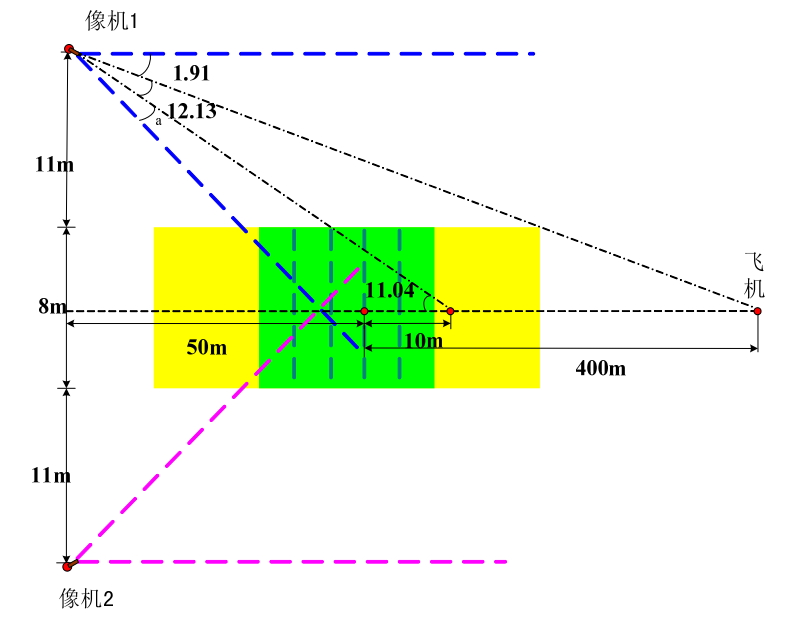
\includegraphics[width=0.6\textwidth]{figs/chp01/chp01_07_ding_master.pdf}
	\caption{地面引导系统排布示意图}
	\label{fig:chp01_07_ding_master}
\end{figure}

此外,该研究组还提出了采用多台固定焦距摄像机分区域接力测量的方案如图\ref{fig:chp01_08_gui_doctor}所示\cite{gui_doctor_2013}。视觉引导系统由三组摄像机选取不同的焦距,分别观测远场、中场和近场区域,保证相邻两组摄像机视场有一定的重叠区域,并覆盖无人机的下降区域。

\begin{figure}[htb]   
	\centering
	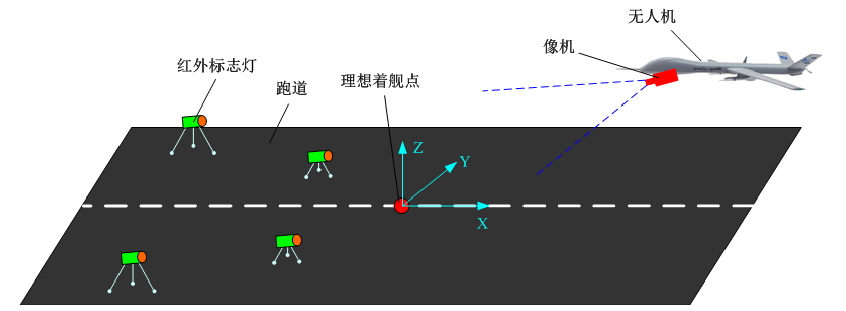
\includegraphics[width=0.6\textwidth]{figs/chp01/chp01_08_gui_doctor.pdf}
	\caption{地基多相机引导系统示意图}
	\label{fig:chp01_08_gui_doctor}
\end{figure}

文献\cite{Garcia-Pardo2002}给出了一种基于步进电机和网络摄像头结合的引导设备,可以对微小型无人机进行跟踪,但其视场角受到步进电机的约束。Martinez\cite{Martinez2010}提出了一种三目摄像机系统,如图\ref{fig:chp01_09_three_ground_landing}所示,该系统可以检测无人机的特征点,得到位置信息,但由于构型限制,该系统只适用于旋翼直升机的降落。美国斯坦福大学(Stanford University)\cite{Saripalli2003}使用两个或以上的相机得到了距离$40\ m$外,位置误差约$25\ cm$的视觉系统,但文献中没有具体描述系统的具体结构。日本千叶大学(Chiba University)的研究者\cite{PEBRIANTI2010}使用利用Bumblebee立体视觉传感器,成功将一架四悬翼从$6\ m$的高度引导降落。

\begin{figure}[htb]   
	\centering
	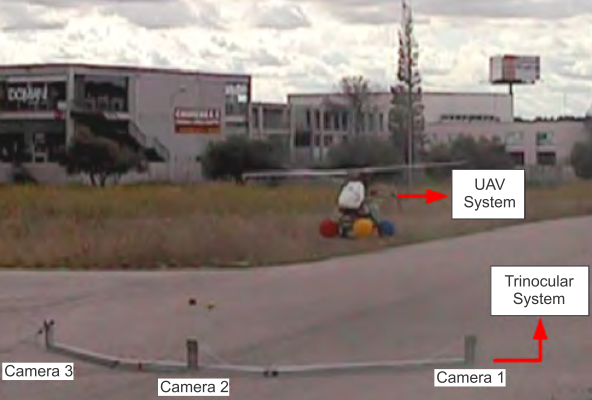
\includegraphics[width=0.7\textwidth]{figs/chp01/chp01_09_three_ground_landing.pdf}
	\caption{地面引导系统排布示意图}
	\label{fig:chp01_09_three_ground_landing}
\end{figure}

\section{本文的主要工作、贡献和结构}
本文瞄准固定翼无人机着舰回收的实际需求,重点研究着舰引导控制的系统架构、机理建模、关键算法与综合验证,主要工作和贡献如下:

(1)提出一种舰基通用的多传感器无人机回收引导系统。该系统主要有两个独立引导单元组成,每个引导单元配备一个二自由度转台和可见光相机、红外相机等多个传感器。两个独立引导单元的排布可以根据目标无人机的大小和检测距离进行优化配置。本文针对该系统独立分布在跑道两侧的特点,通过对目标位置解算理论推导、误差分析和实验验证,证明了在无人机降落过程中,使用上述引导系统的可行性。

(2)提出检测-跟踪-学习相融合的无人机降落过程中实时目标跟踪和位置解算框架。针对引导无人机降落过程中,无人机目标尺度快速变化问题,通过改进基于形态学滤波的图像预处理方法,TLD目标跟踪框架和基于主动轮廓的目标位置修正方法,结合转台运动位置和无人机运动的估计,能够准确解算出无人机在降落过程中相对于舰船的位置信息,满足无人机引导和控制系统的需要。

(3)设计基于非线性模型预测控制(NMPC)和总能量控制(TESC)的无人机着舰控制系统。由于无人机机载设备运算能力的约束,本文设计了内环控制器和外环控制器来实现无人机的自主降落。其中内环控制器由PI和PD控制器组成,完成对无人机姿态的控制;外环控制器由非线性模型预测控制器(NMPC)和总能量控制器(TESC)组成,针对基于Dubins Path生成的降落曲线进行跟踪。

(4)设计并实现无人机舰载着舰系统仿真环境并进行户外实验验证。本文基于机器人操作系统(Robot Operating System,ROS)和Gazebo仿真环境构建了无人机舰载着陆软件在回路仿真系统(SITL)和硬件在回路仿真系统(HIL)。该仿真环境能够满足上述算法的验证需求。通过二自由度转台与多传感器的组合配置,实现在地面机场和水面环境对小型和中型固定翼无人机的引导和自主降落。

本文各个章节的结构图如图\ref{fig:chp01_10_thesis_structure}所示。
\begin{figure}[!h]   
	\centering	
	\includegraphics[width=\textwidth]{figs/chp01/chp01_10_thesis_structure.pdf}
	\caption{本文的组织结构图}
	\label{fig:chp01_10_thesis_structure}
\end{figure}

 	\chapter{无人机着舰环境数学建模}
\label{chap:main}
无人机着舰的过程设计到无人机系统和舰船系统两大部分,因此为了研究这两部分直接的关系,必须对降落过程进行适当的数学模型\cite{beardsmall},以利于对无人机控制和引导系统进行数学仿真和物理实验。

\section{无人机系统坐标系定义}


\subsection{系统惯性坐标系}
系统惯性坐标系(Inertial Frame,$\mathcal{F}^i$),该坐标系一般定义位于地球表面的一点,三个轴的方向$(\mathbf{i}^i, \mathbf{j}^i,\mathbf{k}^i)$与地球的北向、动向和指向地心方向相同,即NED坐标系。通常该坐标系定义为飞机的起飞点或降落点,本文中我们选用无人机被舰船引导系统捕获时,舰船的此刻所在的点为原点,如图\ref{fig:chp02_01_sys_interial_frame}所示。
\begin{figure}[htb]   
	\centering
	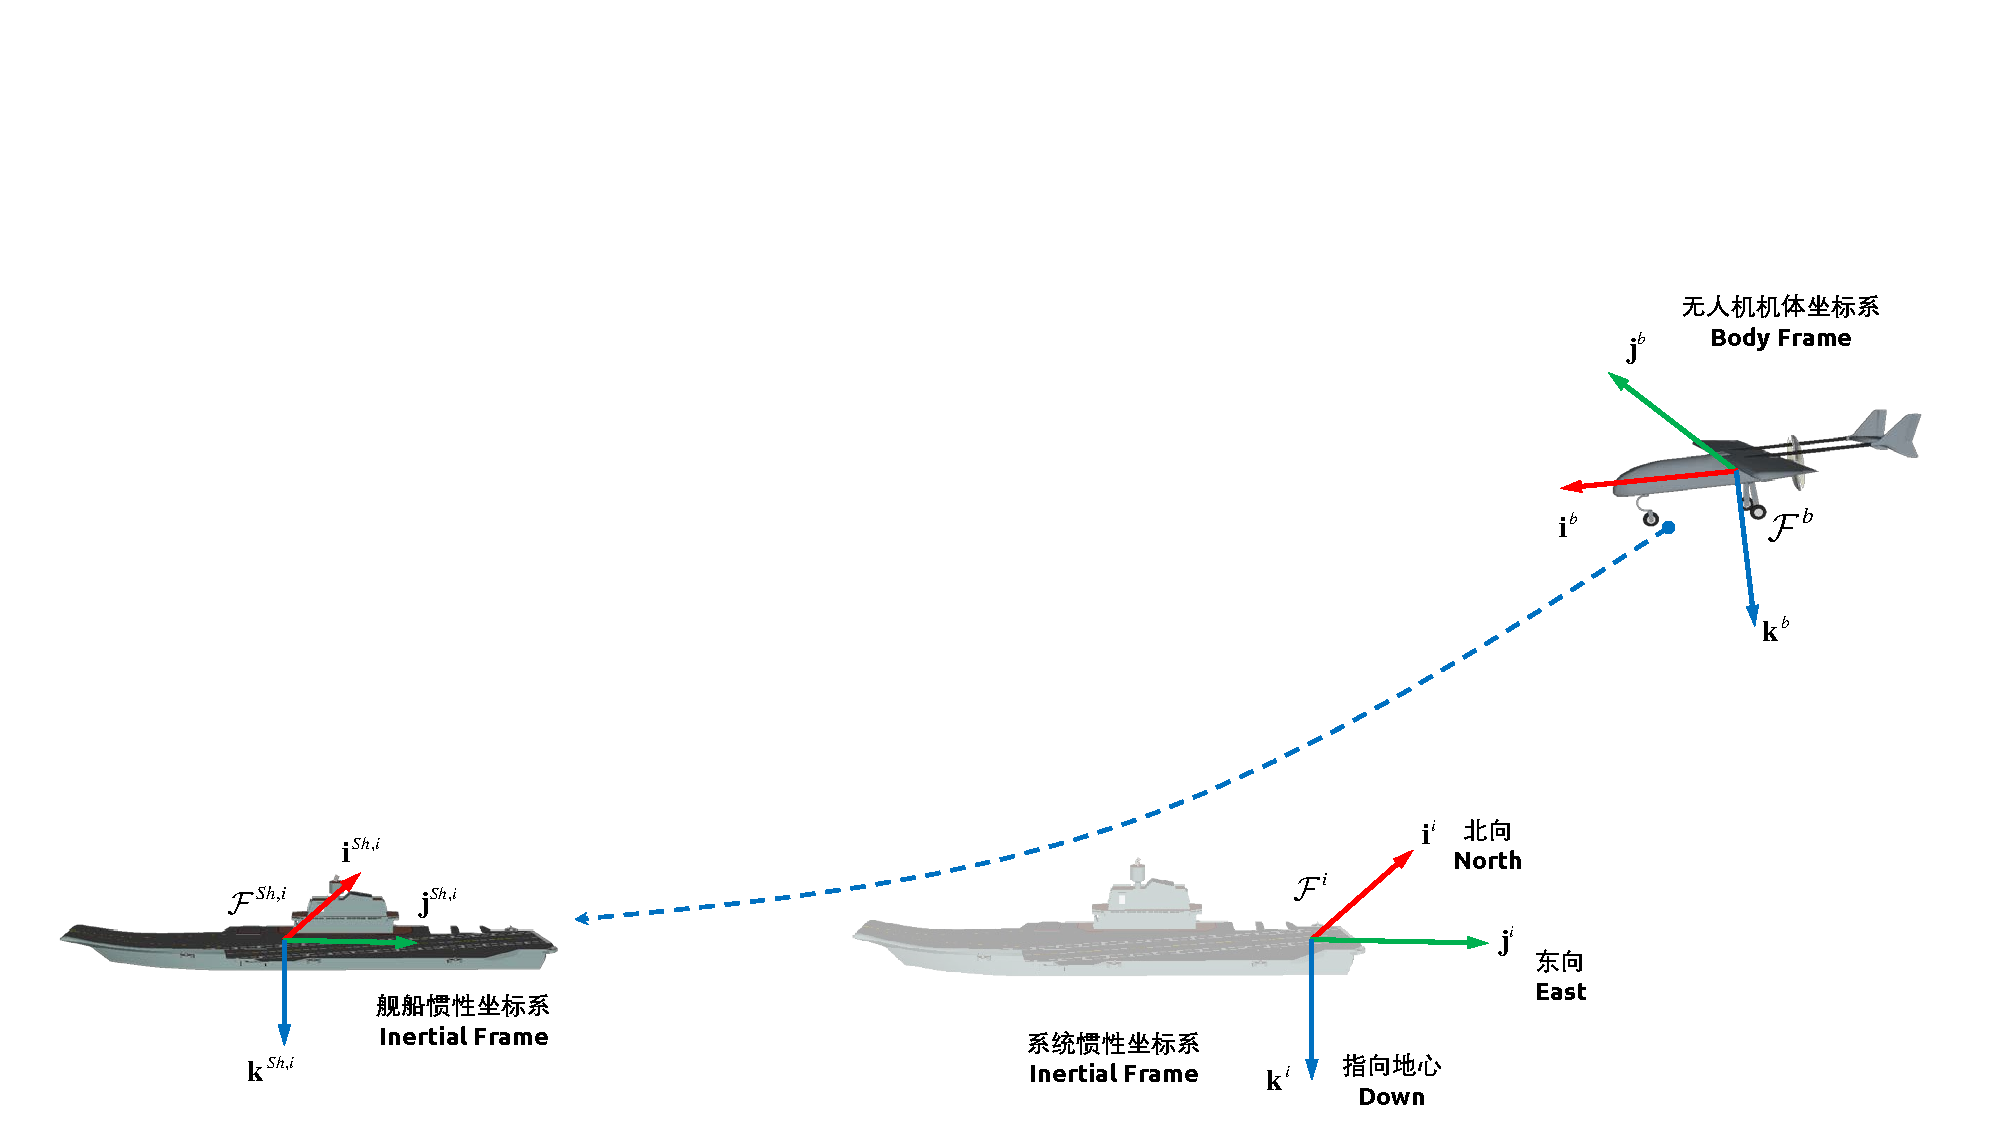
\includegraphics[width=\textwidth]{figs/chp02/chp02_01_sys_interial_frame.pdf}
	\caption{系统惯性坐标系}
	\label{fig:chp02_01_sys_interial_frame}
\end{figure}

\subsection{无人机惯性坐标系}
无人机惯性坐标系($\mathcal{F}^v$,Vehicle Inertial Frame),该坐标系的原点位于飞机的重心,三轴方向与系统坐标系平行。

\begin{figure}[htb]   
	\centering
	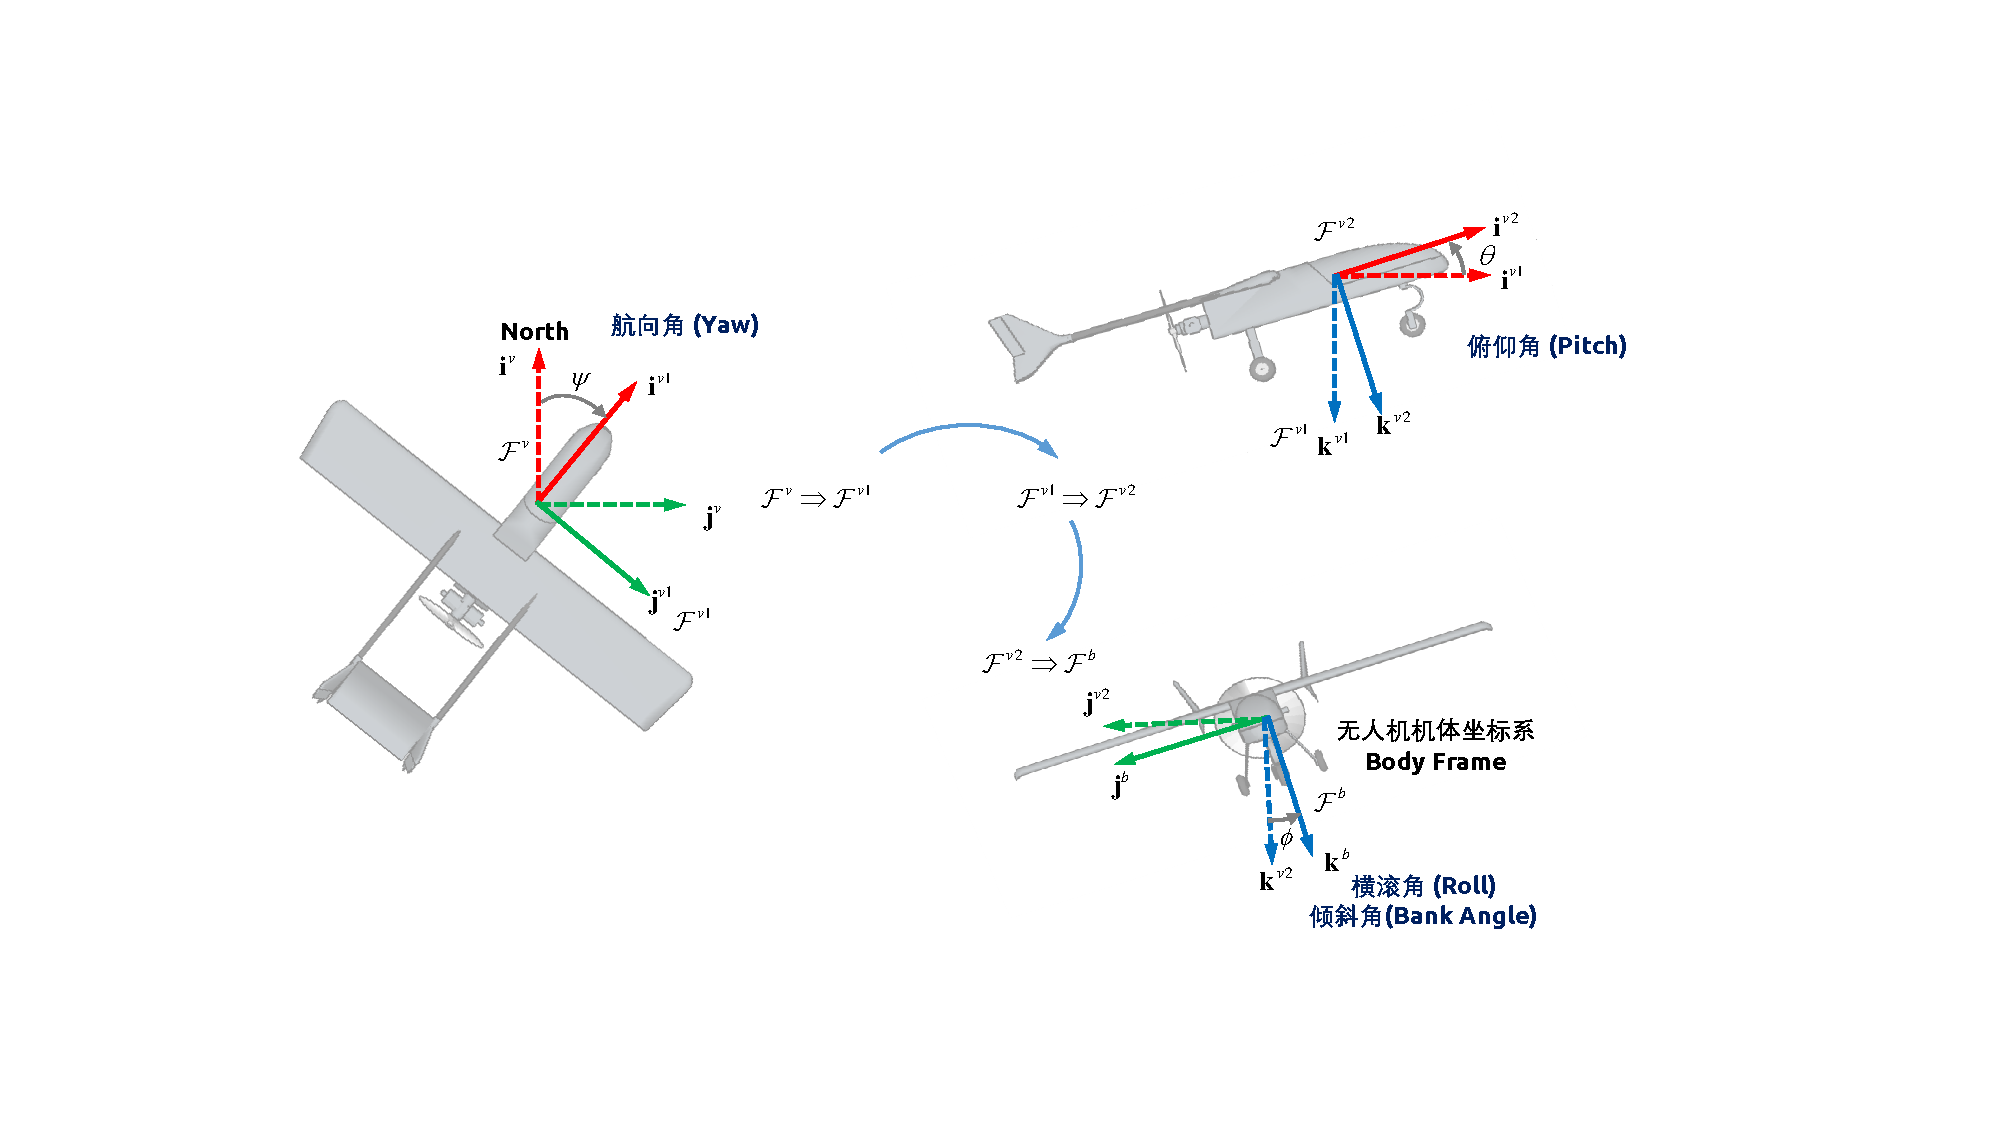
\includegraphics[width=\textwidth]{figs/chp02/chp02_02_uav_rpy.pdf}
	\caption{无人机机体坐标系与横滚角、俯仰角和偏航角定义}
	\label{fig:chp02_02_uav_rpy}
\end{figure}

无人机第一惯性辅助坐标系($\mathcal{F}^{v1}$ ),该坐标系绕无人机惯性坐标系$\mathbf{k}^v$轴按右手规则旋转得到,其中旋转角度定义为$\psi$,即偏航角(Yaw Angle)。

无人机第二惯性辅助坐标系($\mathcal{F}^{v2}$),该坐标系过绕人机第一惯性辅助坐标系$\mathbf{j}^{v1}$轴按右手规则旋转旋转得到,其旋转角度定义为$\theta$,即俯仰角(Pitch Angle)。

无人机机体坐标系($\mathcal{F}^b$,Body Frame ),该坐标系绕无人机第二惯性辅助坐标系$\mathbf{i}^{v2}$轴按右手规则旋转旋转得到,其旋转角度定义为$\phi$,即横滚角(Roll Angle),有时该角度也被称为倾斜角(Bank Angle)。上述四个坐标系之间的转换关系如图\ref{fig:chp02_02_uav_rpy}所示。

根据上述四个坐标系的几何关系,可以得到由机体惯性坐标系$\mathcal{F}^v$转换到机体坐标系$\mathcal{F}^b$的转换矩阵为
\begin{multline}
\mathcal{R}_v^b(\phi, \theta, \psi) =\mathcal{R}_{v2}^b(\phi)\mathcal{R}_{v1}^{v2}(\theta)\mathcal{R}_v^{v1}(\psi) \\
=\begin{bmatrix}
\cos \theta \cos \psi                             & \cos\theta \sin\psi                               & -\sin\theta         \\
-\cos\phi \sin\psi + \sin\phi \sin\theta \cos\psi & \cos\phi \cos\psi + \sin\phi \sin\theta\sin\psi   & \sin\phi \cos\theta \\
\sin\phi \sin\psi + \cos\phi \sin\theta \cos\psi  & -\sin\phi \cos\psi + \cos\phi \sin\theta \sin\psi & \cos\phi \cos\theta
\end{bmatrix}
\end{multline}


机体坐标系$\mathcal{F}^b$转换到稳定坐标系$\mathcal{F}^s$的转换矩阵为
\begin{equation} 
\mathcal{R}_b^s(\alpha) = \begin{bmatrix}
\cos \alpha                             & 0                               & \sin \alpha         \\
0 & 1   &0 \\
-\sin \alpha   & 0 & \cos \alpha
\end{bmatrix}
\end{equation}

稳定坐标系$\mathcal{F}^s$转换为风坐标系$\mathcal{F}^w$的转换矩阵为
\begin{equation} 
\mathcal{R}_s^w(\beta) = \begin{bmatrix} \sin \beta  & \cos \beta  &  0      \\  - \sin \beta & \cos \beta   &0 \\  0   & 0 &1  \end{bmatrix}
\end{equation}

风坐标系$\mathcal{F}^w$转换为机体坐标系$\mathcal{F}^b$转换矩阵为

\begin{equation} 
\mathcal{R}_w^b (\alpha,\beta) = \begin{bmatrix} \cos \beta \cos \alpha & - \sin \beta \cos \alpha  & - \sin \alpha      \\	 \sin \beta & \cos \beta   & 0 \\	\cos \beta   & -\sin \beta \sin \alpha & \cos \alpha \end{bmatrix}
\end{equation}

\subsection{无人机风向坐标系}
无人机风向坐标系($\mathcal{F}^w$,Wind Frame),该坐标系的$\mathbf{i}^w$轴与风速方向相同,可以通过旋转稳定坐标系的$\mathbf{k}^s$轴$\beta$角度得到,该角度$\beta$被定义为侧滑角。无人机攻角和侧滑角的定义如图\ref{fig:chp02_03_uav_aoa_bank}所示。
\begin{figure}[htb]   
	\centering
	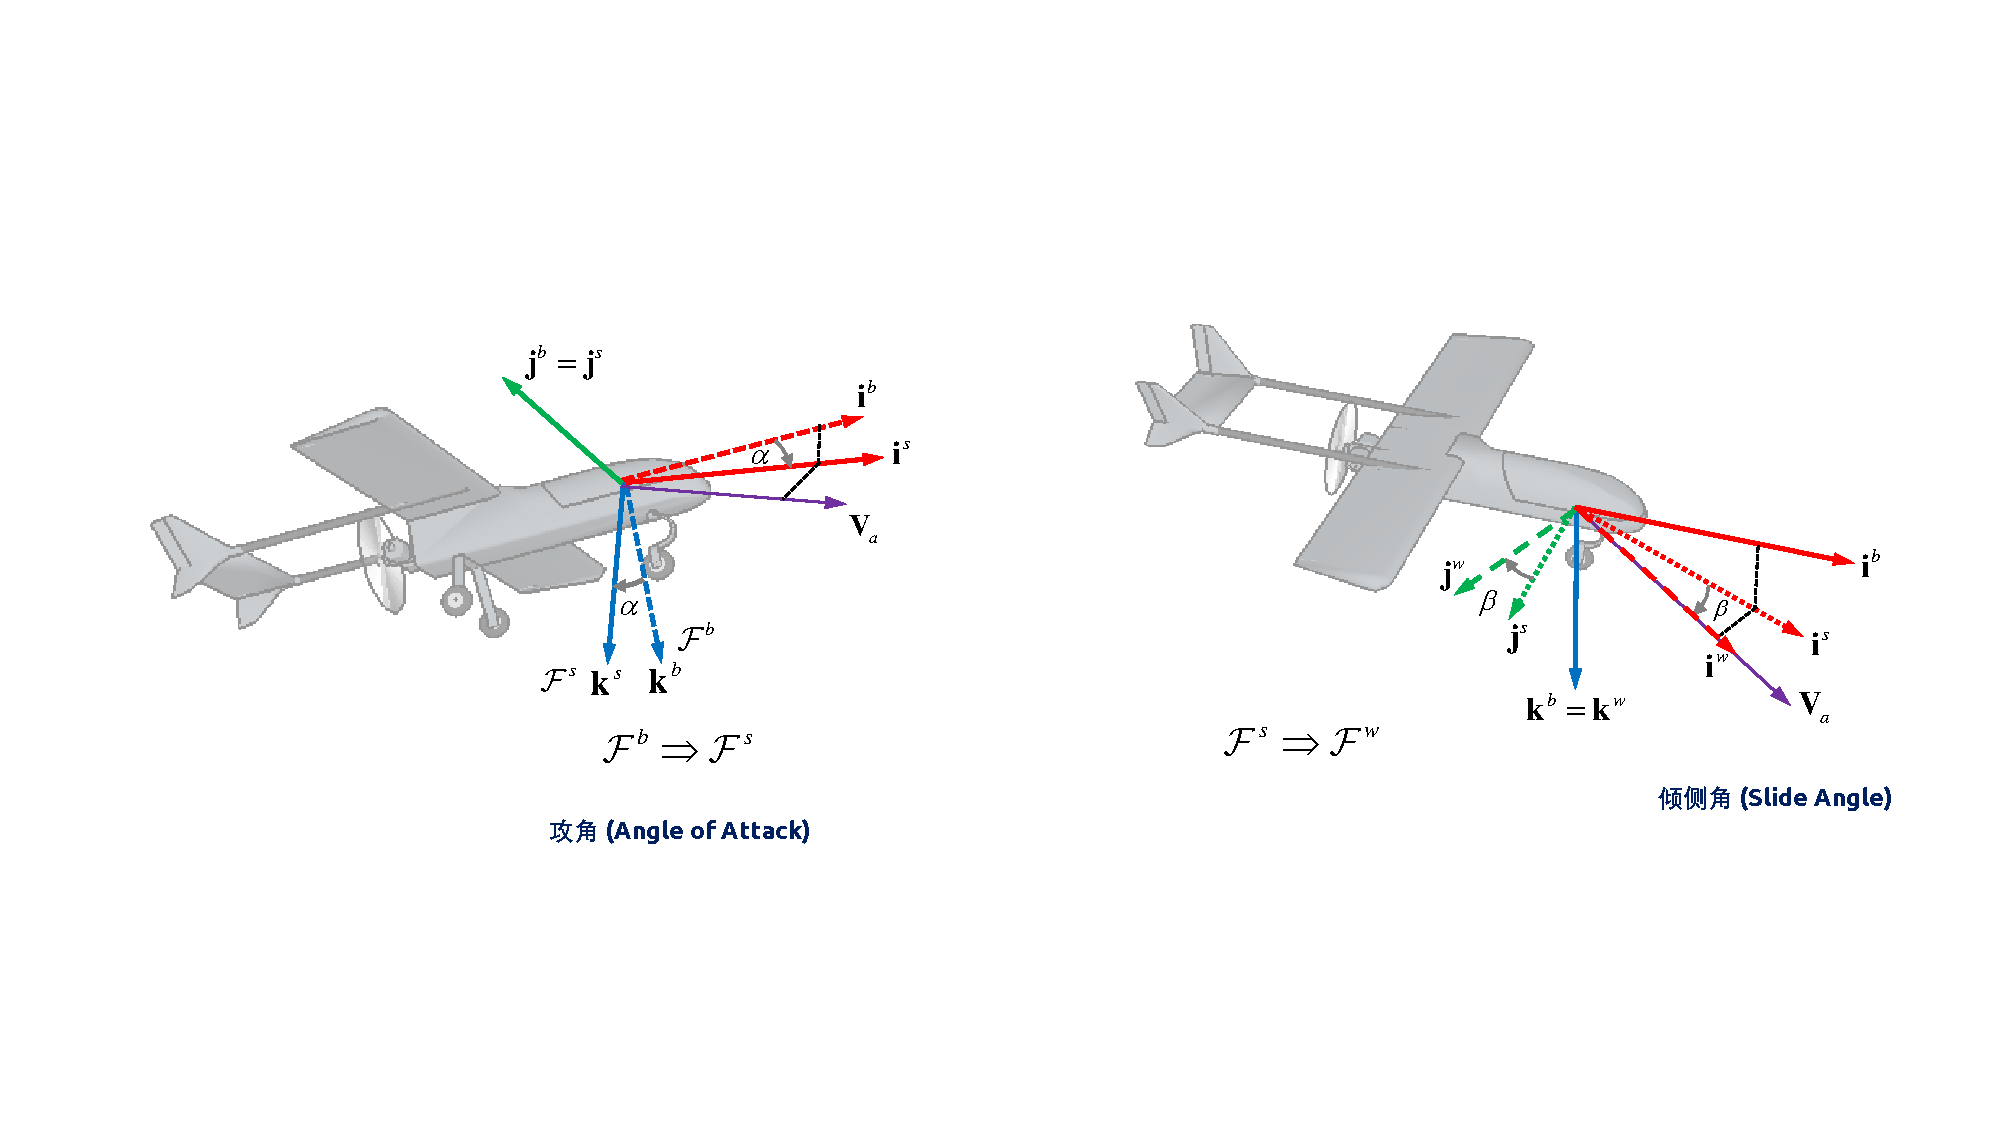
\includegraphics[width=\textwidth]{figs/chp02/chp02_03_uav_aoa_bank.pdf}
	\caption{无人机稳定坐标系与攻角、侧滑角定义}
	\label{fig:chp02_03_uav_aoa_bank}
\end{figure}

\subsection{无人机稳定坐标系}
无人机稳定坐标系($\mathcal{F}^s$,Stability Frame),该坐标系绕无人机机体坐标系$\mathbf{j}^b$按左手规则旋转得到,该坐标系表达如图\ref{fig:chp02_03_uav_aoa_bank}。其中,定义无人机相对于机体周边空气的速度向量为$\mathbf{V}_a$,其大小为$V_a$。为使机翼产生升力,机翼与风速的夹角必须为正,该角度定义为攻角。这里使用左手系的原因是为更方便的定义定义攻角$\alpha$的正负,即沿稳定坐标系$\mathbf{j^s}$按右手系转动到机体坐标系的角度为正。稳定坐标系的$\mathbf{i}^s$轴与空速向量$\mathbf{V}_a$在$\mathbf{i}^b$-$\mathbf{k}^b$的投影方向平行。

定义$\mathbf{V}_a$为空速(Airspeed),即无人机相对于周边流体的速度。
该向量在风坐标系$\mathcal{F}^w$的表达为
\begin{equation} 
\mathbf{V}_a^w=\begin{bmatrix} V_a \\ 0 \\ 0 \end{bmatrix}
\end{equation}
该向量在机体坐标系$\mathcal{F}^b$的表达为
\begin{equation} 
\mathbf{V}_a^b = \begin{bmatrix} u_r \\ v_r \\ w_r \end{bmatrix}
\end{equation}

$\mathbf{V}_g$定义为地速(Ground Speed),即无人机相对于系统惯性系的速度
无人机相对于惯性系的速度该向量在机体坐标系$\mathcal{F}^b$的表达为
\begin{equation}
\mathbf{V}_g^b=\begin{bmatrix} u \\ v \\w \end{bmatrix}
\end{equation}

$\mathbf{V}_w$定义为风速(Wind Speed),即风相对于系统惯性系的速度。
风速在机体坐标系$\mathcal{F}^b$的表达为
\begin{equation}
\mathbf{V}_w^b=\begin{bmatrix} u_w \\ v_w \\w_w \end{bmatrix} \\
=\mathcal{R}_v^b(\phi, \theta, \psi) \begin{bmatrix} w_n \\ w_e \\ w_d \end{bmatrix}
\end{equation}
其中$(w_n, w_e, w_d)$是风速在无人机惯性坐标系的表达。
上述三个速度直接的关系为
\begin{equation}
\mathbf{V}_a = \mathbf{V}_b - \mathbf{V}_w
\end{equation}

上述三个关系的表达如图\ref{fig:chp02_04_uav_wind_frame}所示,根据上述关系,可以得到风速在机体坐标系的另一个表达
\begin{equation}
\mathbf{V}_a^b  = \begin{bmatrix} u_r \\ v_r \\ w_r \end{bmatrix} =   \begin{bmatrix} u - u_w \\ v - v_w \\ w- w_w \end{bmatrix}
\end{equation}
根据风坐标系$\mathcal{F}^w$与$\mathcal{F}^b$机体坐标系的转换关系,风速在机体坐标系还可以表达为
\begin{equation}
\mathbf{V}_a^b  = \begin{bmatrix} u_r \\ v_r \\ w_r \end{bmatrix} \\
=  \mathcal{R}_w^b \begin{bmatrix} V_a \\ 0 \\ 0 \end{bmatrix} \\
=  \begin{bmatrix}	\cos \beta \cos \alpha & - \sin \beta \cos \alpha  & - \sin \alpha      \\	 \sin \beta & \cos \beta   & 0 \\ 	\cos \beta   & -\sin \beta \sin \alpha & \cos \alpha \end{bmatrix} \begin{bmatrix} V_a \\ 0 \\ 0 \end{bmatrix}
\end{equation}
由此可以得到上式更简便的表达
\begin{equation}
\begin{bmatrix} u_r \\ v_r \\ w_r \end{bmatrix}  = {V}_a \begin{bmatrix} \cos \alpha \cos \beta \\ \sin \beta  \\ \sin \alpha \cos \beta \end{bmatrix}
\end{equation}
注意,此处的$V_a$是风速向量的标量。

在已知风速相对于机体坐标系的向量表达时,可以进一步得到风速、攻角和侧滑角的计算
\begin{align}
V_a &= \sqrt{(u_r)^2+(v_r)^2+(w_r)^2} \\
\alpha &=  \tan^{-1}\frac{w_r}{u_r}  \\
\beta  &=  \sin^{-1} \big( \frac{u_r}{\sqrt{(u_r)^2+(v_r)^2+(w_r)^2}} \big)
\end{align}

\begin{figure}[htb]   
	\centering
	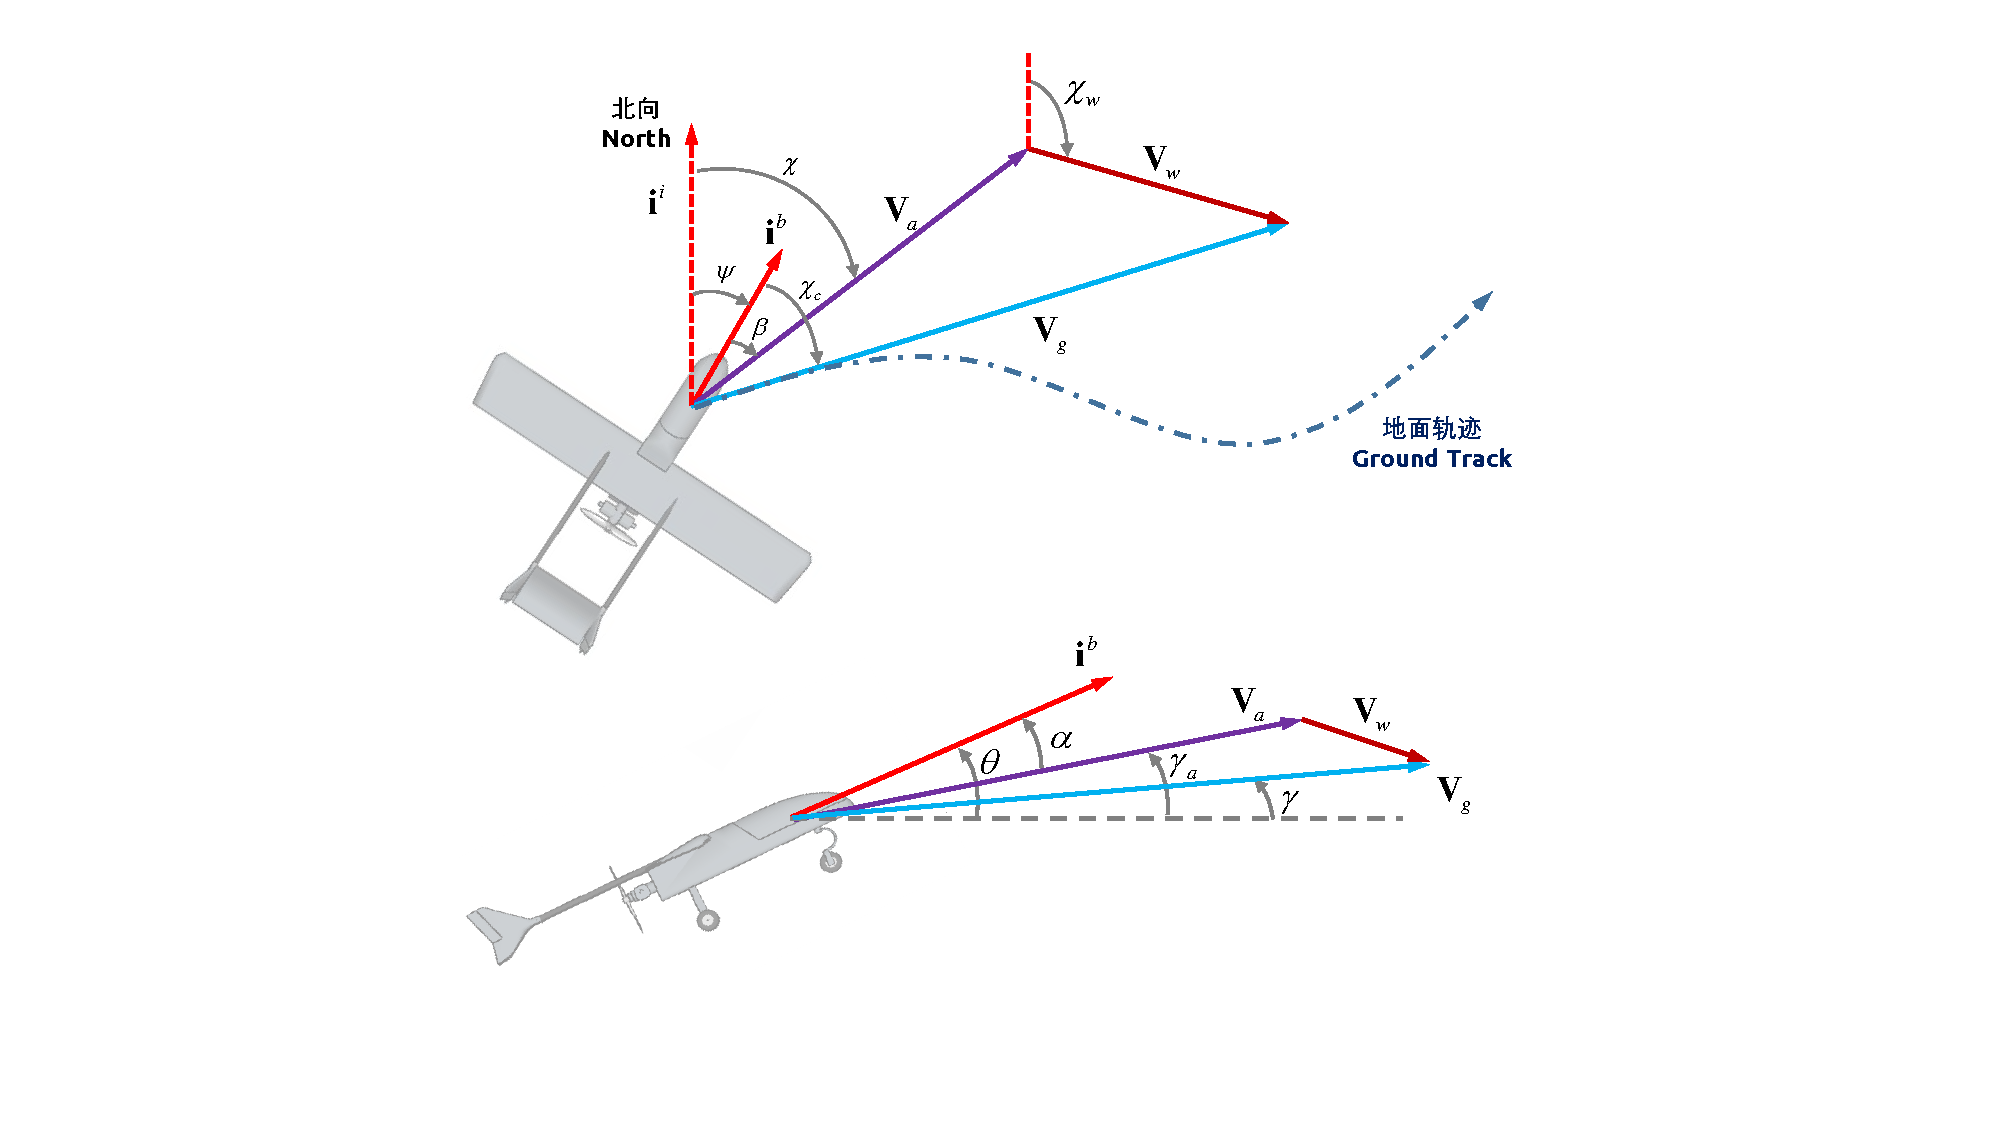
\includegraphics[width=0.8\textwidth]{figs/chp02/chp02_04_uav_wind_frame.pdf}
	\caption{无人机地速、风速和空速三角形}
	\label{fig:chp02_04_uav_wind_frame}
\end{figure}

 




\section{无人机系统运动学和动力学分析}
\subsection{三维空间向量微分}
假设在机体坐标系$\mathcal{F}^b$存在一个运动的向量$\mathbf{p}$,如图\ref{fig:chp02_06_vector_rotation}所示,该向量的数学表达为 
\begin{equation}
\mathbf{p }= p_x \mathbf{i}^b +  p_y \mathbf{j}^b +  p_z \mathbf{k}^b
\end{equation}
\begin{figure}[htb]   
	\centering
	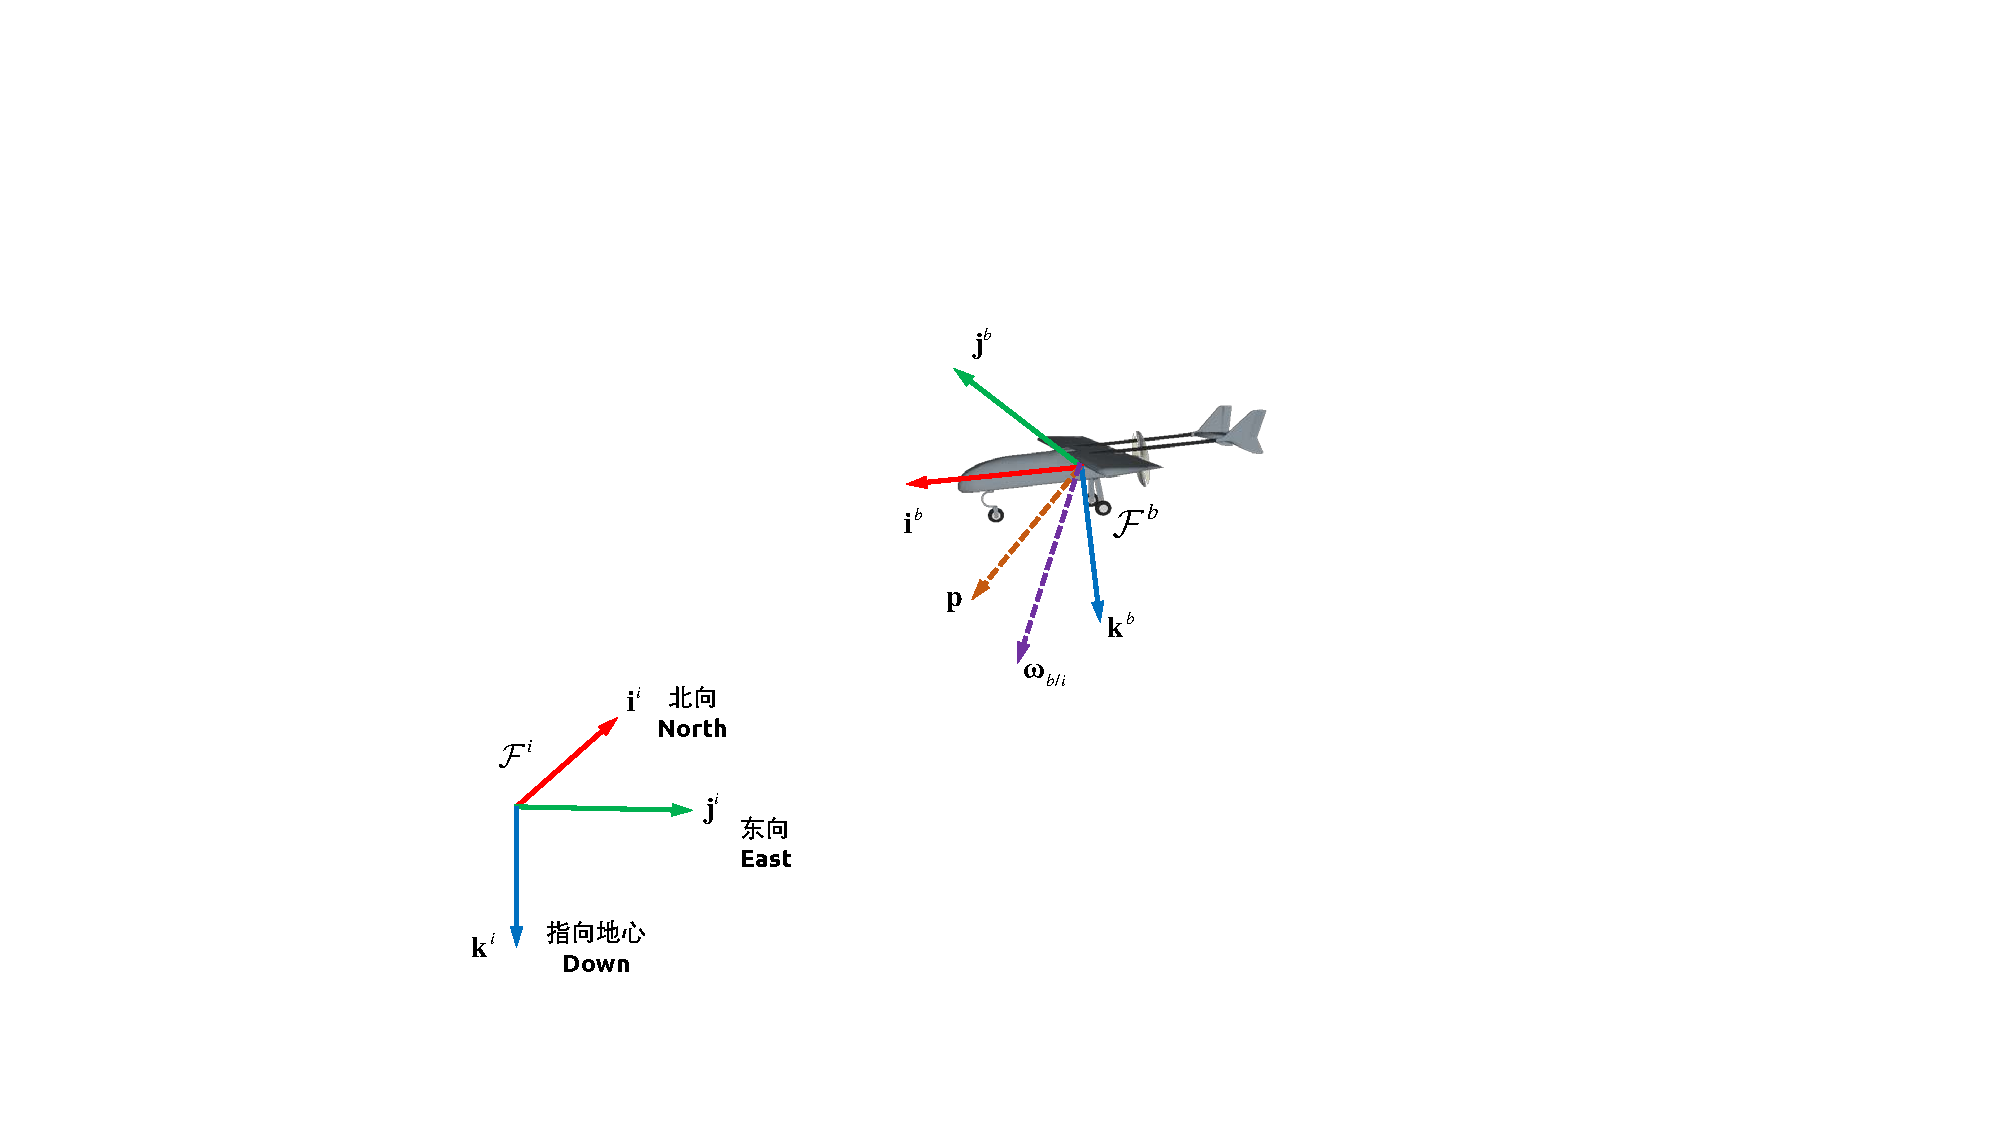
\includegraphics[width=0.8\textwidth]{figs/chp02/chp02_06_vector_rotation.pdf}
	\caption{三维空间向量微分}
	\label{fig:chp02_06_vector_rotation}
\end{figure}

此时机体坐标系$\mathcal{F}^b$与惯性坐标系$\mathcal{F}^i$只存绕转动向量$\mathbf{\omega}_{b/i}$的转动,不存在平动。由此得到该运动向量$\mathbf{p}$相对于系统坐标系$\mathcal{F}^i$的微分为
\begin{equation} \label{chp02_vector_derivative}
\frac{d}{dt_i} \mathbf{p} = \frac{d}{dt_b} \mathbf{p} + \mathbf{\omega}_{b/i} \times \mathbf{p}
\end{equation}
其中等式右侧的第一项具体表达为
\begin{equation}
\frac{d}{dt_i} \mathbf{p} = \dot{p}_x \mathbf{i}^b +  \dot{p}_y \mathbf{j}^b +  \dot{p}_z \mathbf{k}^b
\end{equation}
该部分可以通过设计无人机状态的观测器的获得。

\subsection{无人机空间位置定义}
因为飞机着舰过程的运动范围相对较小,由此对问题的坐标的整体构架主要选用Flat-Earth模型来替代WGS-84模型。首先,对于无人机在系统惯性系$\mathcal{F}^i$的位置定义为$(p_n\ p_e\ p_d)^T$,其中$n$, $e$  和$d$ 描述系统坐标系正北、正东和指向地心的方向。定义$h = -p_d$,用于描述无人机的飞行高度。无人机在系统惯性系的速度在机体坐标系$\mathcal{F}^b$的投影为$(u, v, w)$,无人机在机体坐标系$\mathcal{F}^b$的旋转角速度为$(p, q, r)$。则可以得到无人机速度在两个坐标系的相互转换关系
\begin{equation}
\frac{d}{dt} \begin{bmatrix} p_n \\ p_e \\ p_d \end{bmatrix}   =  (\mathcal{R}_v^b)^T \begin{bmatrix} u \\  v \\ w \end{bmatrix}  
\end{equation}
\begin{equation}
\resizebox{.9 \textwidth}{!} 
{ $
\begin{bmatrix} \dot{p}_n \\ \dot{p}_e \\ \dot{p}_d \end{bmatrix} = \begin{bmatrix}  cos \theta \cos \psi   &     -\cos\phi \sin\psi + \sin\phi \sin\theta \cos\psi                        &  \sin\phi \sin\psi + \cos\phi \sin\theta \cos\psi       \\
\cos\theta \sin\psi    & \cos\phi \cos\psi + \sin\phi \sin\theta\sin\psi   & -\sin\phi \cos\psi + \cos\phi \sin\theta \sin\psi \\
-\sin\theta  & \sin\phi \cos\theta & \cos\phi \cos\theta
\end{bmatrix} \begin{bmatrix} u \\  v \\ w \end{bmatrix}
$}
\end{equation}
进一步化解可以得到
\begin{align}
\begin{bmatrix} p \\ q \\ r \end{bmatrix}  &=   \begin{bmatrix}
1 &  0   & -\sin \theta      \\
0 &  \cos \phi  & \sin \phi \cos \theta \\	
0 & -\sin \phi   & \cos \phi \cos \theta
\end{bmatrix} \begin{bmatrix} \dot{\phi} \\ \dot{\theta} \\ \dot{\psi} \end{bmatrix} \\
\begin{bmatrix} \dot{\phi} \\ \dot{\theta} \\ \dot{\psi} \end{bmatrix}  &=  \begin{bmatrix}
1 &  \sin \phi \tan \theta  & - \cos \phi \tan \theta      \\
0 & \cos \phi   & -\sin \phi \\
0  & \sin \phi \sec \theta & \cos \phi \sec \theta
\end{bmatrix} \begin{bmatrix} p \\ q \\ r \end{bmatrix}
\end{align}

\subsection{无人机的外部力和力矩分析}
无人机的质量定义为$\mathsf{m}$,所受全部外力定义为$\mathbf{f}$,主要由重力$\mathbf{f}_g$、空气动力$\mathbf{f}_a$和电机拉力$\mathbf{f}_p$三部分组成
\begin{equation}
\mathbf{f} = \mathbf{f}_g + \mathbf{f}_a + \mathbf{f}_p
\end{equation}

重力在无人机惯性坐标系$\mathcal{F}^v$的表达为
\begin{equation}
\mathbf{f}_g^v = \begin{bmatrix}0  \\ 0  \\ \mathsf{m}g  \end{bmatrix}
\end{equation}

重力在无人机机体坐标系$\mathcal{F}^b$的表达为
\begin{equation}
\mathbf{f}_g^b =\mathcal{R}^b_v \begin{bmatrix}0  \\ 0  \\ \mathsf{m}g  \end{bmatrix} \\
= \begin{bmatrix} -\mathsf{m} g \sin \theta  \\ \mathsf{m}g \cos \theta \sin \phi  \\ \mathsf{m}g \cos\theta \cos \phi  \end{bmatrix}
\end{equation}

根据空气动力定义,在水平方向,无人机受到的升力$F_{lift}$、阻力$F_{drag}$和力矩$m$,其基本定义为
\begin{align}
F_{filt} = \frac{1}{2} V_a^2SC_L(\alpha, q, \delta_e) \\
F_{drag} = \frac{1}{2} V_a^2SC_D(\alpha, q, \delta_e) \\
m = \frac{1}{2} V_a^2ScC_m(\alpha, q, \delta_e)
\end{align}
其中$S$是机翼面积,$c$是机翼平均舷长,$C_L$、$C_D$和$C_m$是非线性空气动力参数。此外,无人机的控制面为三个,副翼偏移$\delta_a$,方向舵偏移$\delta_r$和升降舵偏移$\delta_e$。

根据本文目标无人机的空气特性,由此将上述气动力参数进一步展开为
\begin{align}
C_L(\alpha, q, \delta_e) &= C_X(\alpha) + {C_X}_q(\alpha) \frac{c}{2V_a}  q+ C_{X_{{\delta}_e}}(\alpha) \delta_e \\
C_D(\alpha, q, \delta_e) &= C_{Y_{0}} + C_{Y_{\beta}} \beta + C_{Y_r}(\alpha) \frac{b}{2V_a} r+ C_{Y_{\delta_\alpha}} \delta_\alpha +  C_{Y_{\delta_r}} \delta_r  \\ 
C_m(\alpha, q, \delta_e) &= C_Z(\alpha) + C_{Z_q}(\alpha) \frac{c}{2V_a}  q+ C_{Z_{\delta_e}} \delta_e
\end{align}
其中
\begin{align}
C_X(\alpha) &= -C_D(\alpha) \cos \alpha +  C_L(\alpha) \sin \alpha \\
C_{X_q}(\alpha) &= -C_{D_q} \cos \alpha +  C_{L_q} \sin \alpha \\
C_{X_{\delta_e}}(\alpha) &= -C_{D_{\delta_e}} \cos \alpha +  C_{L_{\delta_e}} \sin \alpha \\
C_Z(\alpha) &= -C_D(\alpha) \cos \alpha -  C_L(\alpha) \sin \alpha \\
C_X(\alpha) &= -C_{D_q} \sin \alpha -  C_{L_q} \cos \alpha \\
C_X(\alpha) &= -C_{D_{\delta_e}}  \sin \alpha -  C_{L_{\delta_e}} \cos \alpha \\
\end{align}
因为升力和阻力作用在无人机稳定坐标系$\mathcal{F}^s$上,因此将上述力转换到无人机的机体坐标系后,进一步得到
\begin{align}
\begin{bmatrix} f_x    \\ f_z  \end{bmatrix} = \begin{bmatrix}
\cos \alpha    & - \sin \alpha  \\
\sin \alpha       & \cos \alpha  \\
\end{bmatrix} \begin{bmatrix} -F_{drag}    \\ -F_{lift}  \end{bmatrix}
\end{align}
在竖直方向,无人机受到竖直方向的力和力矩为
\begin{align}
f_y = \frac{1}{2} \rho V_a^2 S C_y (\beta, p, r, \delta_a, \delta_r) \\
l  = \frac{1}{2} \rho V_a^2 S b  C_l (\beta, p, r, \delta_a, \delta_r) \\
n = \frac{1}{2} \rho V_a^2 S b C_n (\beta, p, r, \delta_a, \delta_r)
\end{align}
其中,$C_y$、$C_l$和$C_n$是非线性空气动力参数。

螺旋桨的推力建模为
\begin{equation}
\mathbf{f}_p = \frac{1}{2} \rho S_{prop} C_{prop}  \begin{bmatrix} (\mathsf{k}_{motor} \delta_t)^2 - V_a^2  \\ 0  \\ 0  \end{bmatrix}
\end{equation}
其中$\mathsf{k}_{motor}$是电机效率常数,$\delta_t$是电机的控制量,$S_{prop}$是螺旋桨的面积,$C_{prop}$是螺旋桨参数。

螺旋桨的力矩建模为
\begin{equation}
\mathbf{T}_p = -\mathsf{k}_{T_p} (\mathsf{k}_{\Omega} \delta_{t})^2
\end{equation}

其中$\Omega = \mathsf{k}_{\Omega} \delta_{t}$是螺旋桨的转速,$\mathsf{k}_{T_p}$是电机常数。

\subsection{无人机的平动分析}
对于无人机的平动,无人机的质量为$\mathsf{m}$和其受到的全部外力$\mathbf{f}$,根据顿第二定律可以得到
\begin{equation}
\mathsf{m} \frac{d \mathbf{V}_g}{d t_i} = \mathbf{f}
\end{equation}
代入\ref{chp02_vector_derivative}公式,可以得到
\begin{equation}
\mathsf{m}(\frac{d \mathbf{V}_g }{dt_b}+ \mathbf{\omega}_{b/i} \times \mathbf{V}_g)=\mathbf{f}
\end{equation}
同理,在机体坐标系$\mathcal{F}^b$可以得到
\begin{equation}
\mathsf{m}(\frac{d \mathbf{V}^b_g }{dt_b}+ \mathbf{\omega}_{b/i}^b \times \mathbf{V}^b_g)=\mathbf{f}^b
\end{equation}
其中$\mathbf{V}_g^b=(u, v, w)^T$描述无人机惯性系的速度向量在机体坐标系的表达,$\frac{d \mathbf{V}_g }{dt_b}=(\dot{u}, \dot{v}, \dot{w})^T$描述无人机速度在机体坐标系的变化率,$\mathbf{\omega}_{b/i}^b=(p, q, r)^T$描述无人机机体坐标系的转动角速度,$\mathbf{f}^b = (f_x, f_y, f_z)^T$描述外部合力向量在机体坐标系的表达。进一步可以得到
\begin{equation}
\begin{bmatrix} \dot{u} \\ \dot{v} \\ \dot{w}  \end{bmatrix} = \begin{bmatrix} rv-qw \\ pw-ru \\ qu-pv  \end{bmatrix} + \frac{1}{\mathsf{m}} \begin{bmatrix} f_x \\ f_y \\ f_z  \end{bmatrix}
\end{equation}



\subsection{无人机的转动分析}
对于无人机对转动,定义角动量$\mathbf{h}$和全部外力矩$\mathbf{m}$,由此可以得到
\begin{equation}
\frac{ d \mathbf{h}}{d t_i}=\mathbf{m}
\end{equation}
同理,对上式求在惯性系的微分
\begin{equation}
\frac{ d \mathbf{h}}{d t_i} = \frac{d\mathbf{h}}{dt_b} + \mathbf{\omega}_{b/i} \times \mathbf{h} = \mathbf{m}
\end{equation}
同理,在机体坐标系的表达为
\begin{equation}
\frac{ d \mathbf{h}^b}{d t_i} = \frac{d\mathbf{h}^b}{dt_b} + \mathbf{\omega}^b_{b/i} \times \mathbf{h}^b = \mathbf{m}^b
\end{equation}
对于刚体来说,角动量的表达通过惯量矩阵$\mathbf{J}$来定义
\begin{equation}
\mathbf{h}^b=\mathbf{J}  \mathbf{\omega}^b_{b/i}
\end{equation}
其中
\begin{align}
\mathbf{J} =\begin{bmatrix}	\int(y^2 + z^2)~d\mathsf{m} & -\int xy \ d\mathsf{m}        & -\int xz~d\mathsf{m} \\	-\int xy~d\mathsf{m}        & \int(x^2 + z^2)~d\mathsf{m} & -\int yz~d\mathsf{m} \\	-\int xz~d\mathsf{m}        & -\int yz~d\mathsf{m}  & \int(x^2 + y^2)~d\mathsf{m} \end{bmatrix}
\end{align}
根据无人机机体的对称性,该矩阵可以化简为
\begin{align}
\mathbf{J} = \begin{bmatrix}	J_x     & 0   & -J_{xz} \\	0       & J_y & 0       \\	-J_{xz} & 0   & J_z  \end{bmatrix}
\end{align}
改矩阵的逆为
\begin{align}
\mathbf{J}^{-1}=\frac{\mathrm{adj}(\mathbf{J}) }{\mathrm{det}(\mathbf{J}) } = \begin{bmatrix}	J_z / \Gamma     & 0   & J_{xz}/ \Gamma \\	0       & 1/ \Gamma & 0       \\	J_{xz}/ \Gamma & 0   & J_z/ \Gamma \end{bmatrix}
\end{align}
其中$ \Gamma = J_xJ_z - J_{xz}^2$ 。

同时,定义上式中的分量
\begin{align}
\dot{\mathbf{\omega}}^b_{b/i}=\frac{ d \mathbf{\omega}^b_{b/i}}{dt_b} = \begin{bmatrix} \dot{p} \\ \dot{q} \\ \dot{r}  \end{bmatrix}
\end{align}
该分量描述在机体坐标系角速度的变化率。

根据上述公式可以得到对角速度变化率的求解
\begin{equation}
\dot{\mathbf{\omega}}^b_{b/i} = \mathbf{J}^{-1}[{- \mathbf{\omega}}^b_{b/i} \times (\mathbf{J{\mathbf{\omega}}^b_{b/i}})+\mathbf{m}^b]
\end{equation}
定义无人机力矩在机体坐标系的表达$\mathbf{m}^b = (l, m, n)$

则可以得到对角速度变化率的进一步表达
\begin{equation}
\begin{bmatrix} \dot{p} \\ \dot{q} \\ \dot{r}  \end{bmatrix} =  \begin{bmatrix} \Gamma_1pq - \Gamma_2qr + \Gamma_3 l + \Gamma_4 n \\ \Gamma_5pr - \Gamma_6(p^2-r^2) + \frac{1}{Jy}m \\ \Gamma_7pq - \Gamma_1qr + \Gamma_4l + \Gamma_8 n  \end{bmatrix}
\end{equation}
其中各个分量的表达为
\begin{align}
\Gamma_1 &= \frac{J_{xz}(J_x-J_y+J_z)}{\Gamma}  \\
\Gamma_2 &= \frac{J_z(J_z-J_y) + J_{xz}^2}{\Gamma}  \\
\Gamma_3 &= \frac{J_z}{\Gamma}  \\
\Gamma_4 &= \frac{J_{xz}}{\Gamma}  \\
\Gamma_5 &= \frac{J_z - J_x}{J_y}  \\
\Gamma_6 &= \frac{J_{xz}}{J_y}  \\
\Gamma_7 &= \frac{(J_x-J_z)J_x+J_{xz}^2}{\Gamma}  \\
\Gamma_8 &= \frac{J_x}{\Gamma}  \\
\end{align}
 
\subsection{无人机运动轨迹数学描述}

\begin{figure}[htb]   
	\centering
	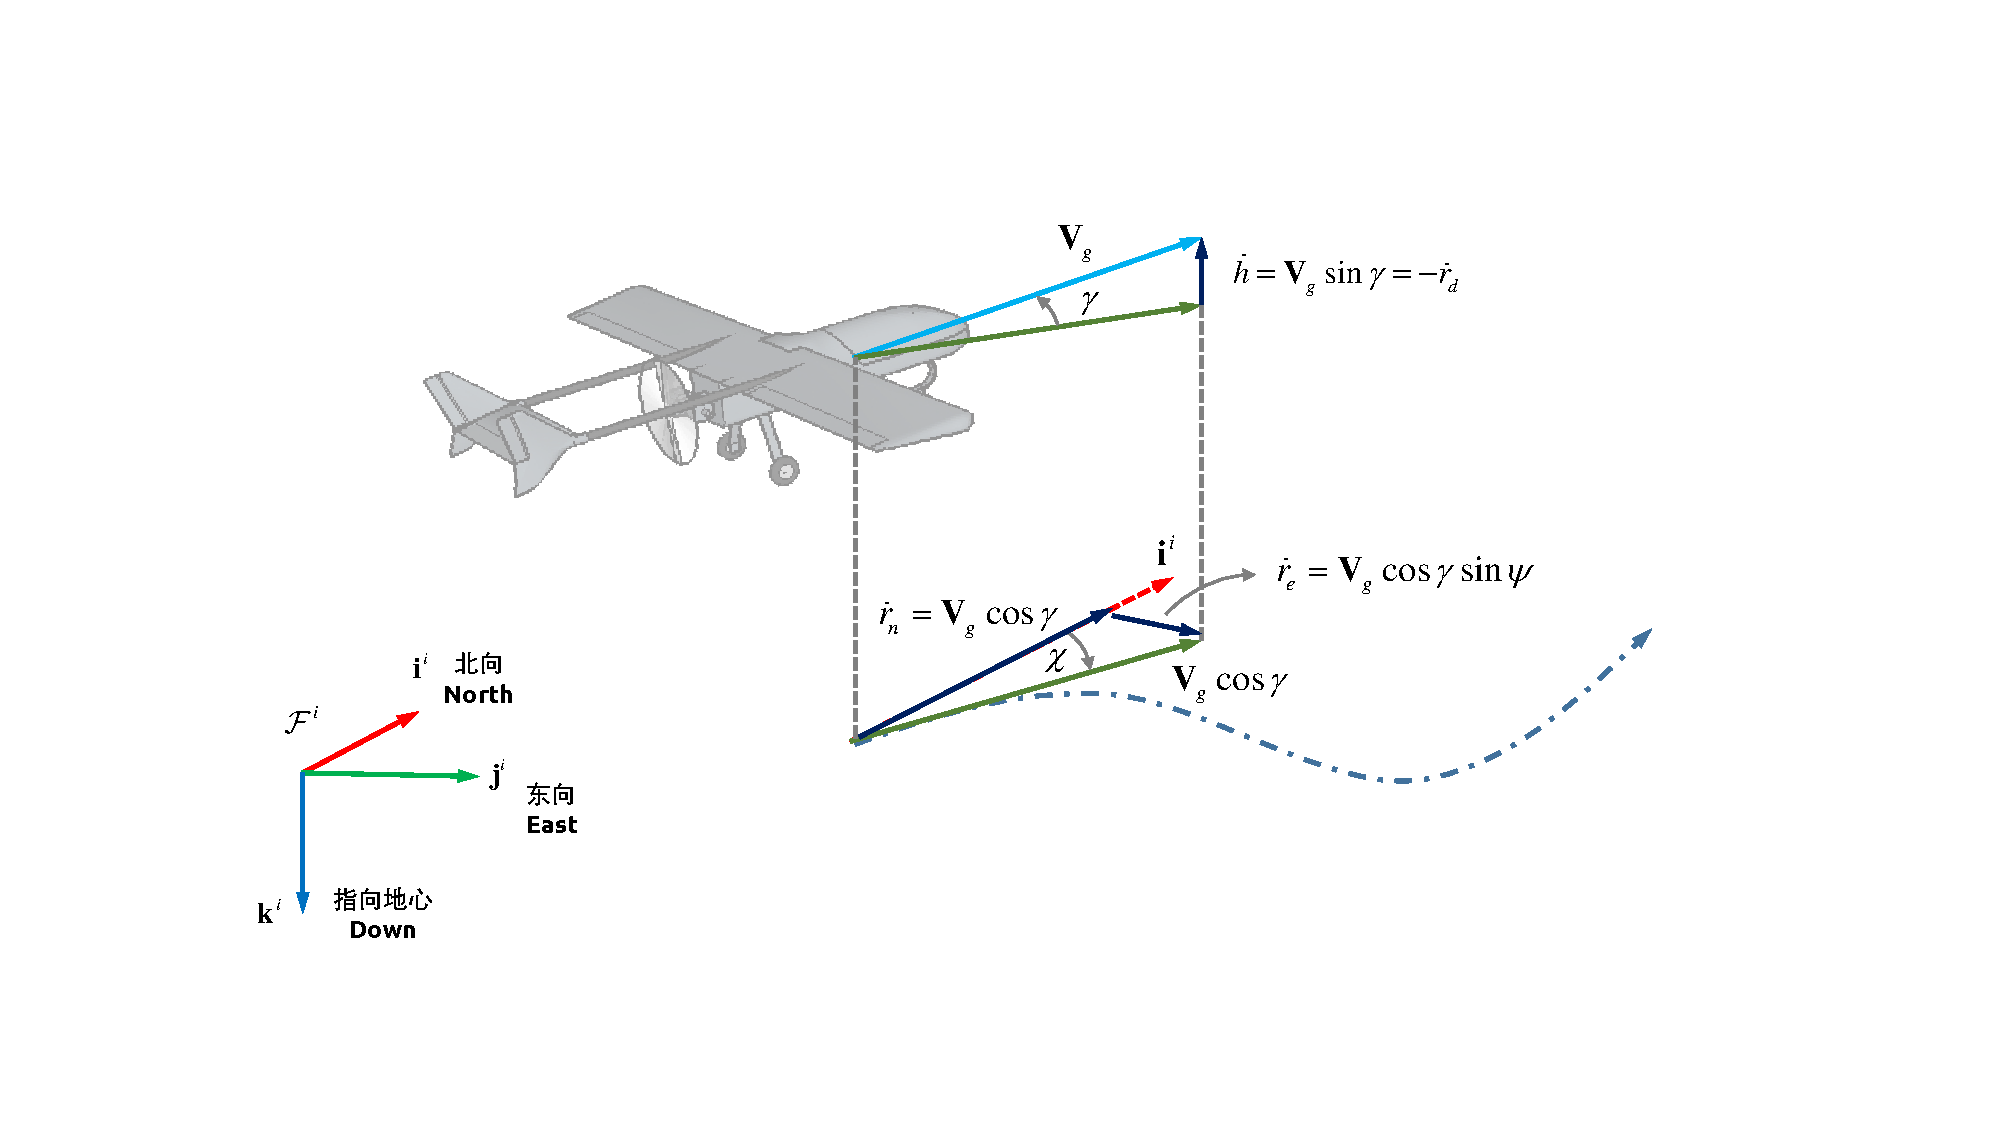
\includegraphics[width=0.8\textwidth]{figs/chp02/chp02_05_uav_course_frame.pdf}
	\caption{无人机运动轨迹描述}
	\label{fig:chp02_05_uav_course_frame}
\end{figure}

定义无人机在惯性系的坐标为$(p_n\ p_e\ p_d)^T$,无人机速度$\mathbf{V}_g$在惯性系的分量为$(\dot{p}_n\ \dot{p}_e\ \dot{p}_d)^T$,该速度的大小用$V_g = ||\mathbf{V}_g||$来表达,如图\ref{fig:chp02_05_uav_course_frame}所示。根据空间几何关系可以得到
\begin{equation}
\begin{bmatrix} \dot{p}_n \\\dot{p}_e \\ \dot{p}_d \end{bmatrix}  = {V}_g \begin{bmatrix} \cos \psi \cos \gamma \\ \sin \psi \cos \gamma  \\- \sin \gamma \end{bmatrix}
\end{equation}
其中航迹角$\gamma$定义为地速$\mathbf{V}_g$与惯性系北向$\mathbf{i}^i$与动向$\mathbf{j}^i$所构成的地平面的夹角,航迹偏航角$\chi$定义为地速$\mathbf{V}_g$在地面投影与正北方向的夹角。

由于无人机受到的升力为$F_{lift}$,在无人机进行协同转向(Coordinated Turn)时,根据力学关系可以得到横向和纵向公式
\begin{align}
&F_{lift} \sin \phi \cos (\chi - \psi) = \mathsf{m} \frac{v^2}{R}  \\
&F_{lift } \cos \phi = \mathsf{m} g \cos \gamma
\end{align}
将上述两式相除,并对$\chi$微分,可以得到
\begin{equation}
\dot{\chi} = \frac{g}{V_g} \tan \phi \cos (\chi - \psi)
\end{equation}
在没有风速影响下($V_g = V_a\ , \psi = \chi$),可以将上式进一步化简为
\begin{equation}
\dot{\psi} =\frac{g}{V_a} \tan \phi
\end{equation}
因为无人机的控制一般分为内环和外环,内环的控制速率较快,即飞行控制器可以很快使得无人机的姿态角收敛到指令期望位置,即$\gamma = \gamma^c\ , \phi = \phi^c$。因此,无人机的运动情况可以通过如下公式进一步描述
\begin{equation}
\begin{bmatrix} \dot{p}_n \\\dot{p}_e \\ \dot{p}_d \end{bmatrix}  = {V}_a \begin{bmatrix} \cos \psi \cos \gamma^c \\ \sin \psi \cos \gamma^c  \\- \sin \gamma^c \end{bmatrix} \\
\dot{\psi} =\frac{g}{V_a} \tan \phi^c
\end{equation}
由于无人机执行机构的物理约束,无人机的控制指令收到进一步约束
\begin{align}
|\phi^c| \le \bar{\phi} \\
|\gamma^c| \le \bar{\gamma}
\end{align}
其中$\bar{\phi}$和$\bar{\gamma}$为无人机系统的最大横滚角和下滑角约束。


\section{舰船系统坐标系定义}

舰船坐标系主要由舰船惯性坐标系、舰船龙骨坐标系和着舰点坐标系三部分组成。
\subsection{舰船惯性坐标系}
舰船惯性坐标系($\mathcal{F}^{Sh,i}$,Ship Inertial Frame),该坐标系的原点定义在舰船的中心位置,一般位于龙骨所在轴线,位于甲板下方。该坐标系的三个轴的方向分别与系统坐标系$\mathcal{F}^i$平行。该坐标系的表达如图\ref{fig:chp02_08_ship_interial_frame}所示。

\begin{figure}[htb]   
	\centering
	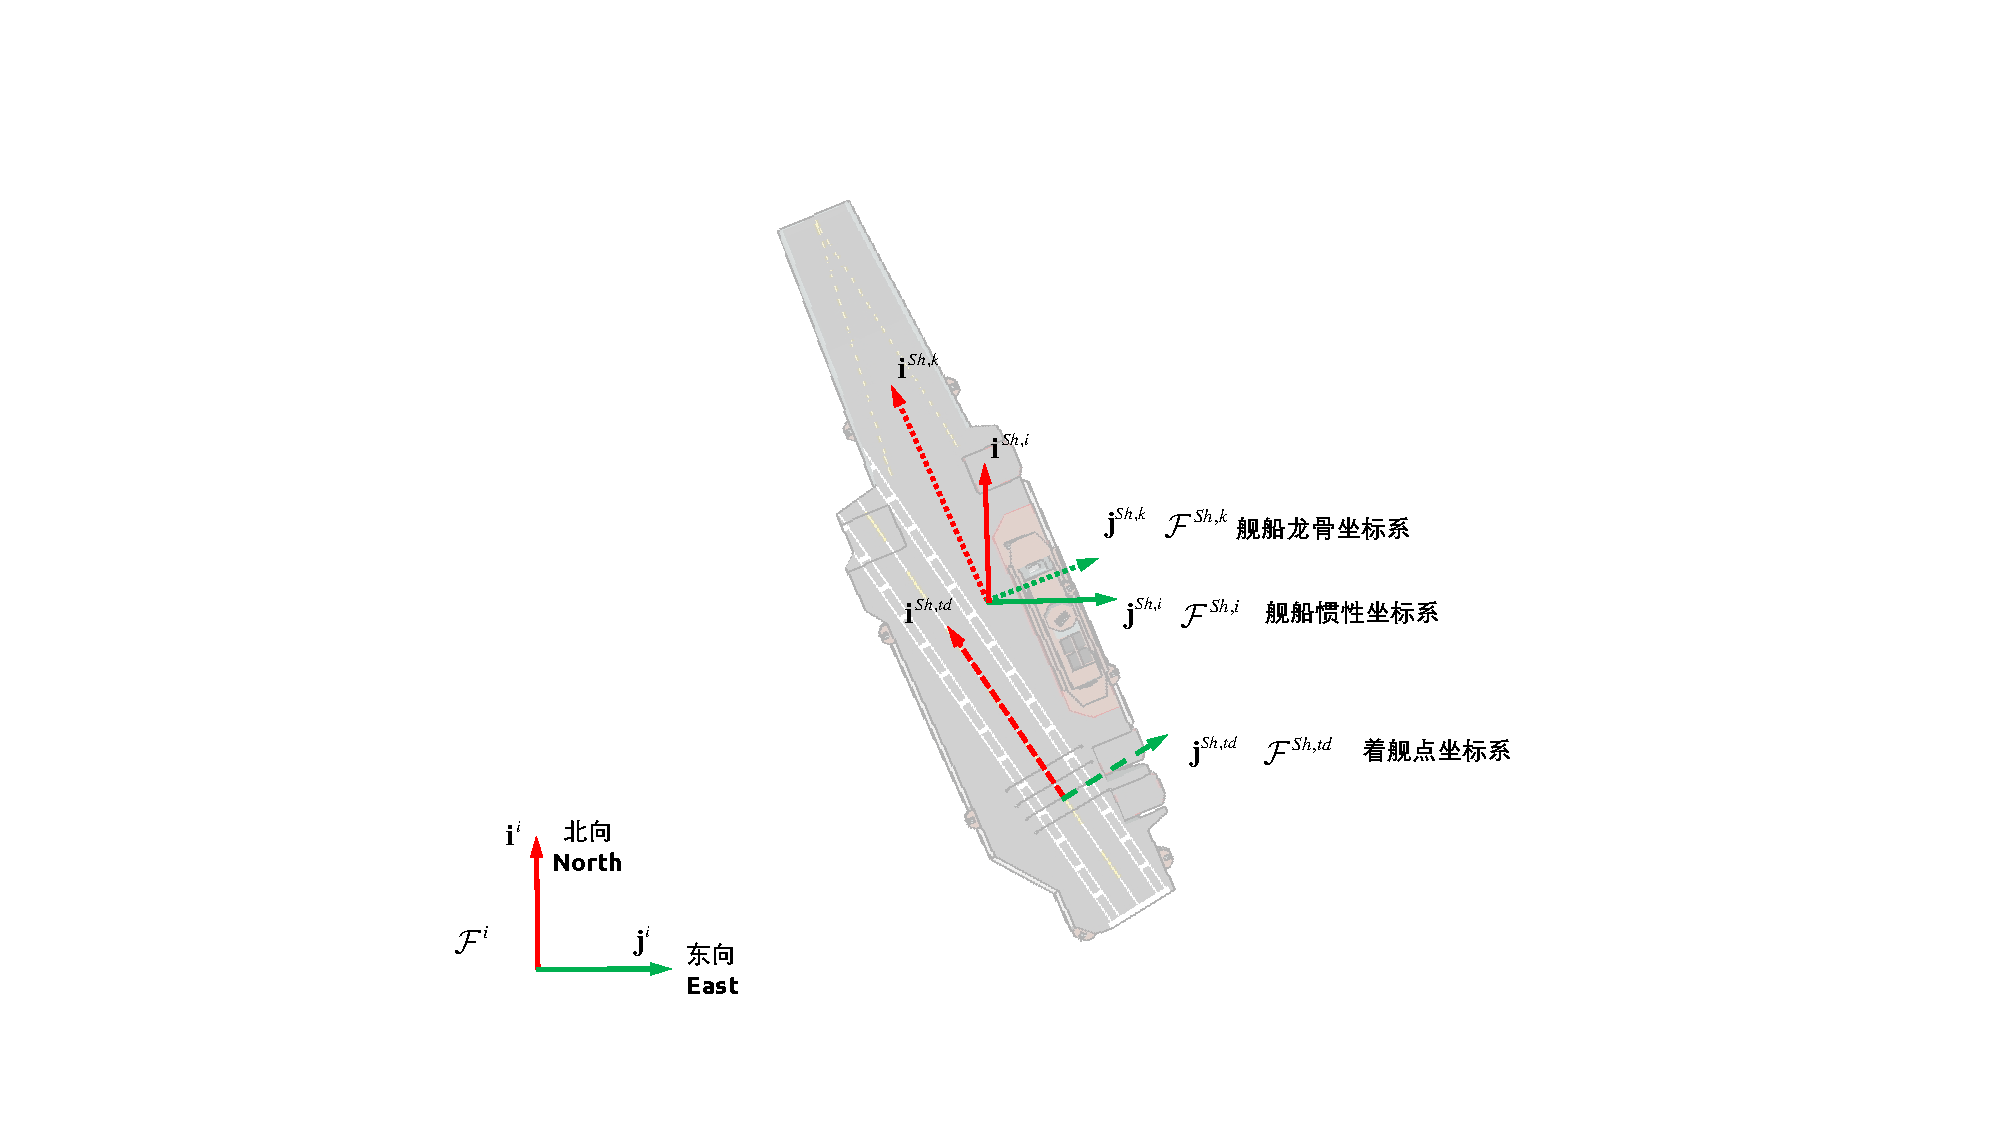
\includegraphics[width=0.8\textwidth]{figs/chp02/chp02_08_ship_interial_frame.pdf}
	\caption{舰船惯性坐标系}
	\label{fig:chp02_08_ship_interial_frame}
\end{figure}

\subsection{舰船龙骨坐标系}
舰船龙骨坐标系($\mathcal{F}^{Sh,k}$ ,Keel Frame),该坐标系的原点与舰船惯性坐标系相同,$\mathbf{i}^{Sh,k}$轴沿龙骨方向指向舰船前进方向,$\mathbf{j}^{Sh,k}$轴垂直于$\mathbf{i}^{Sh,k}$方向。因为该坐标系与船体固连,所以海浪的作用下,该坐标系随船体运动。与无人机机体坐标系类似,将舰船惯性坐标系按照3-2-1的顺序依次旋转至舰船龙骨坐标系,定义三次转动的角度为$\phi_{Sh}$、$\theta_{Sh}$和$\psi_{Sh}$,用于描述舰船的俯仰角、横滚角和偏航角。不同海况情况下,舰船龙骨坐标系还会存在周期性的扰动,由此定义$\Delta \phi_{Sh}$、$\Delta \theta_{Sh}$和$\Delta \psi_{Sh}$来描述舰船龙骨坐标系在俯仰、横滚和偏航三个轴线的扰动角度,定义$\Delta x_{surge}$、$\Delta y_{sway}$和$\Delta z_{heavy}$来描述三个坐标轴的位移偏差,即横摇、纵摇和沉浮。该坐标系的表达如图\ref{fig:chp02_09_ship_motion_frame}所示。

\begin{figure}[htb]   
	\centering
	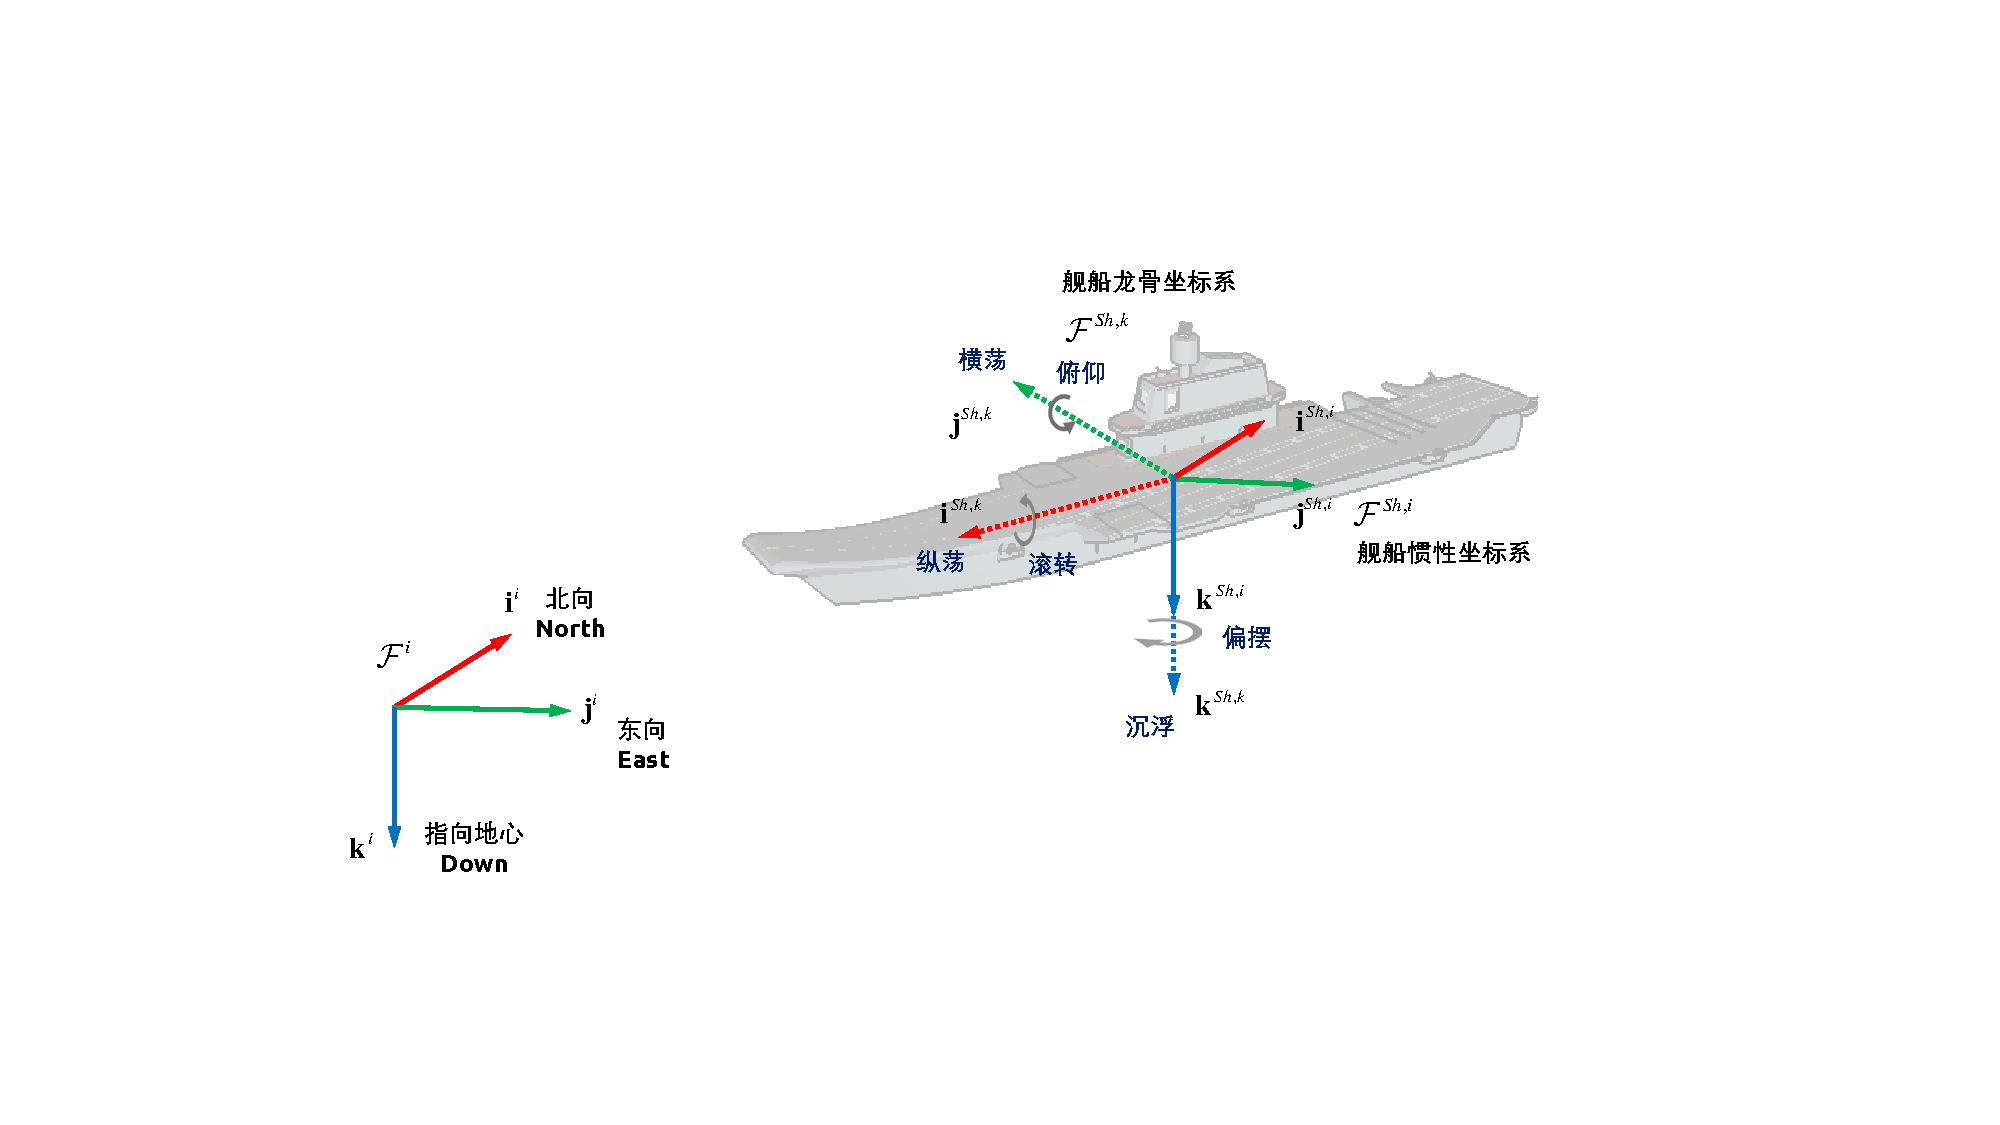
\includegraphics[width=\textwidth]{figs/chp02/chp02_09_ship_motion_frame.pdf}
	\caption{舰船系统坐标系的表达}
	\label{fig:chp02_09_ship_motion_frame}
\end{figure}


\subsection{着舰点坐标系}
着舰点坐标系($\mathcal{F}^{Sh,td}$,Touchdown Frame),该坐标系原点定义在第二条拦阻索的中间位置,$\mathbf{i}^{Sh,td}$轴沿降落跑道指向舰船运行前方,$\mathbf{j}^{Sh,td}$轴沿第二条拦阻索方向延长垂直于$\mathbf{i}^{Sh,td}$轴。

着舰点坐标系与舰船龙骨坐标系之间的转换关系定义为
\begin{equation}
\begin{bmatrix} x_{Sh,td} \\ y_{Sh,td} \\z_{Sh,td} \end{bmatrix} = \begin{bmatrix} x_{Sh,k} \\ y_{Sh,k} \\z_{Sh,k} \end{bmatrix} +\mathcal{R}_{Sh,k}^{Sh,td} \begin{bmatrix} \Delta x_{Sh,k}^{Sh,td} \\ \Delta y_{Sh,k}^{Sh,td} \\ \Delta z_{Sh,k}^{Sh,td} 
\end{bmatrix}
\end{equation}
其中$\Delta x_{Sh,k}^{Sh,td}$,$\Delta y_{Sh,k}^{Sh,td}$和$\Delta z_{Sh,k}^{Sh,td}$是着舰坐标系原点在舰船龙骨坐标系的坐标,$\mathcal{R}_{Sh,k}^{Sh,td}$是从舰船坐标系旋转到着舰点坐标系的旋转矩阵,该旋转矩阵的表达形式与无人机机体惯性坐标系转换到无人机机体坐标系的旋转矩阵相同,$(x_{Sh,k}\ y_{Sh,k}\ z_{Sh,k})$是舰船惯性坐标系上一点,该点在舰船着舰点坐标系上的坐标为$(x_{Sh,td}\ y_{Sh,td}\ z_{Sh,td})$。

\section{舰载引导系统坐标系定义}
由于舰船的运动,对于降落过程中的无人机需要提供有效的局部导航数据,本文设计的舰载引导系统坐标系主要用于描述引导系统对无人机的测量和导航。
\subsection{引导系统坐标系}
引导系统坐标系(Guidance Coordination System, $\mathcal{O}_c$)该坐标系的原点位于左侧引导系统的转台转轴的中心,$\mathbf{i}^{O,c}$轴指向右侧引导系统,并与着舰点坐标系的$\mathbf{j}^{Sh,td}$轴平行,$\mathbf{j}^{O,c}$轴与跑道纵向平行,指向远端无人机方向。该坐标系在舰船运动过程中与甲板固连,与期望着舰点坐标系的位置保持不变。一般而言,对于无人机着舰而言,期望着舰点的位置位于第一道和第二道拦阻索之间,靠近第二道拦阻索,如图\ref{fig:chp02_10_guidance_sys}所示;对于无人机装网回收而言,期望降落位置一般位于无人机回收网的几何中心。
\begin{figure}[htb]   
	\centering
	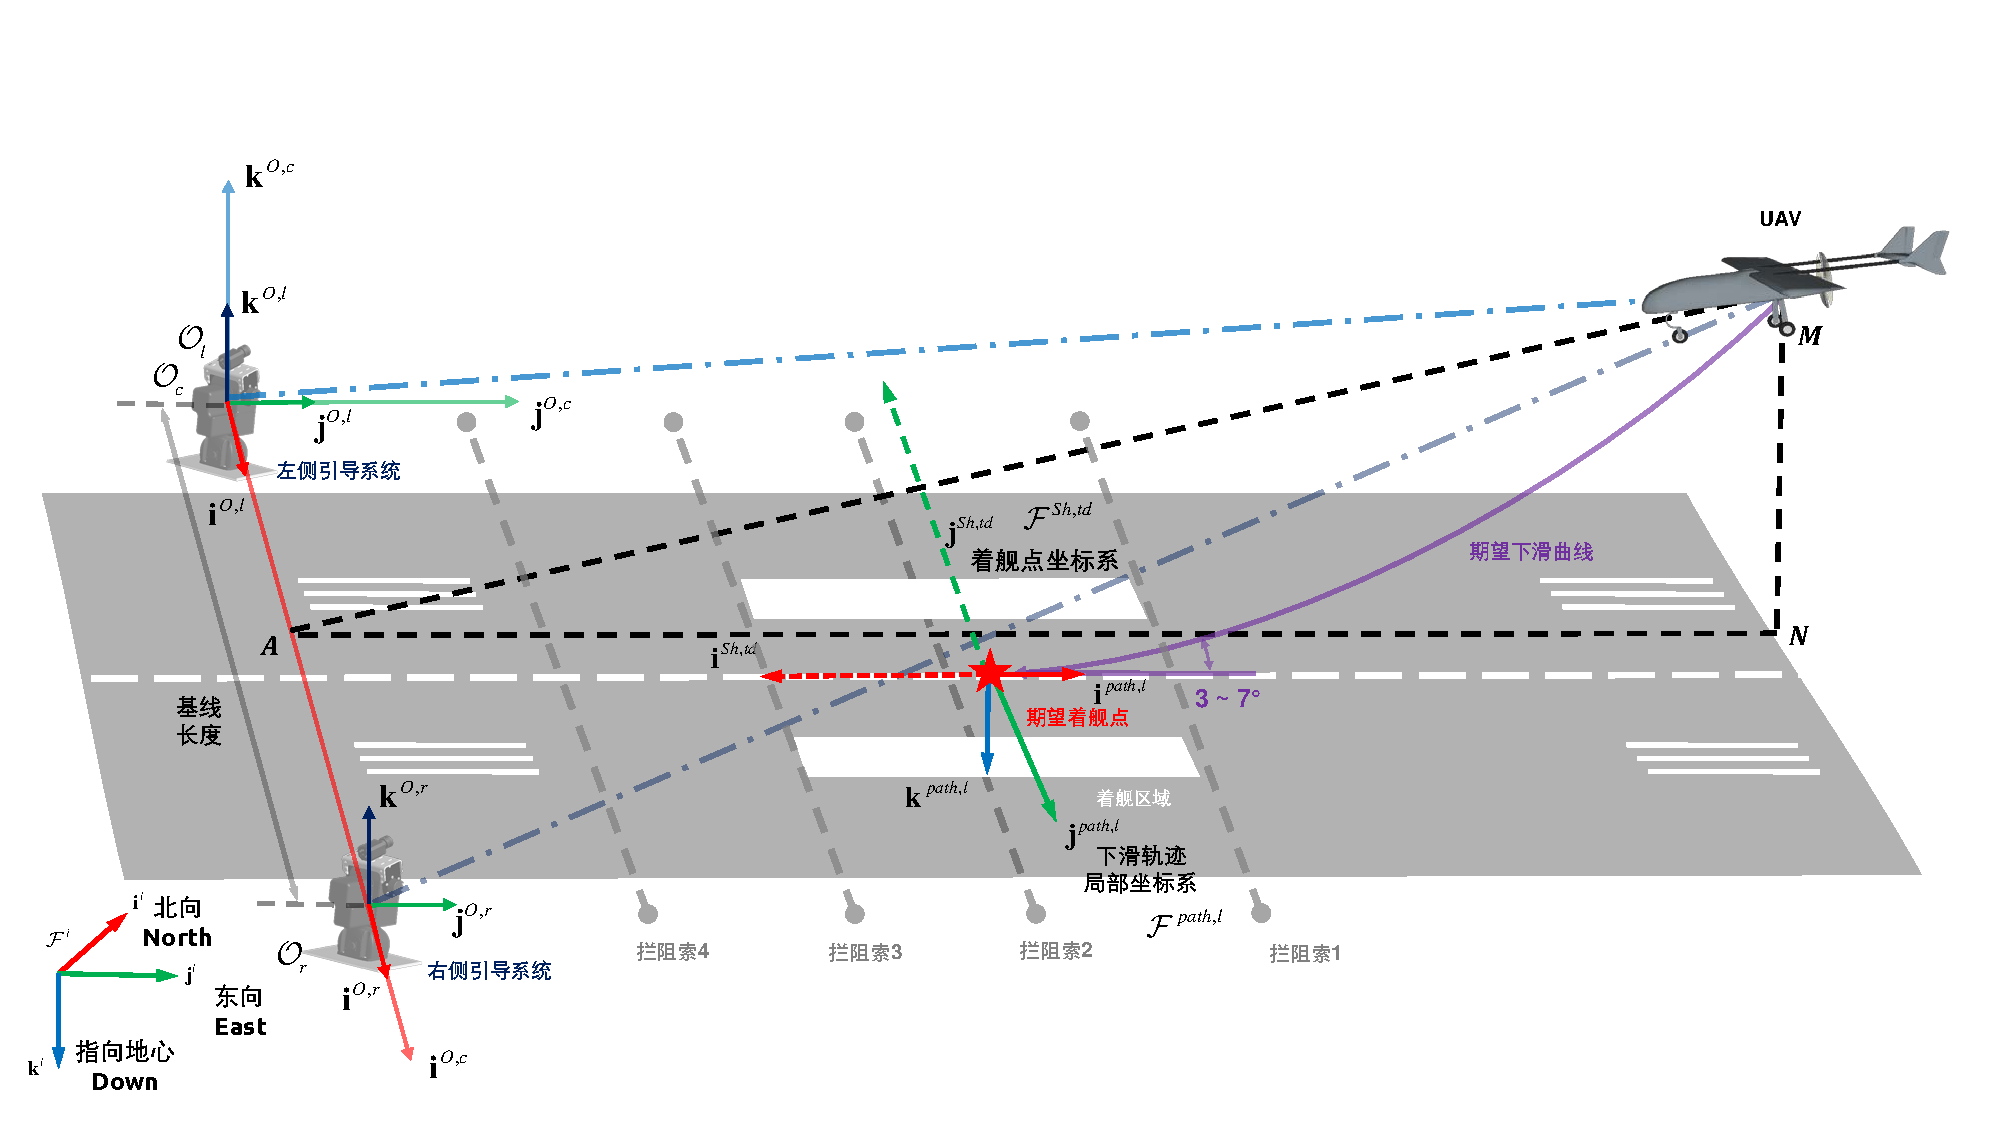
\includegraphics[width=\textwidth]{figs/chp02/chp02_10_guidance_sys.pdf}
	\caption{舰载引导系统相关坐标系}
	\label{fig:chp02_10_guidance_sys}
\end{figure}

\subsection{左右引导单元坐标系}
左侧引导系统坐标系($\mathcal{O}_l$)和右侧引导系统坐标系($\mathcal{O}_r$),这两个坐标系的原点别位于左侧和右侧引导系统的转台转轴中心,三个坐标轴的方向分别与光学引导系统相同。该引导单元坐标系也是用于立体解算无人机空间位置的主要坐标系。

\subsection{地心地固坐标系}
地心地固坐标系(Earth-Centered Earth-Fixed Coordinate System (ECEF),$\mathcal{O}_e$),该坐标系采用1984年\cite{WGS84}指定的地心空间右手坐标系(The World Geodetic System (WGS-84)),原点位于地球中心,$x$轴指向地球0°经线和0°纬线的交叉点,$y$轴指向地球的北极点。该坐标系通常用于大地测量、地图绘制和导航。本文后续试验中使用的该坐标系相关参数为 $R_{Ea}=6,378,137.0\ m$,$R_{Eb} = 6,356,752.0\ m$ ,$f=1/298.257223563$ 和 $e=0.08181919$。

\subsection{GPS坐标系}
GPS坐标系(The Geodetic Coordination System,$\mathcal{O}_g$)中的任意一点通常用$(\lambda\ \varphi\ h)$表示,其中 $\lambda$ 表示目标当前位置的经度, $\varphi$ 表示目标当前位置的纬度, $h$ 表示当前位置的高度。该数值一般通过GPS解算模块获得。

\subsection{GPS坐标系与地心地固坐标系之间的转换关系}
定义GPS经纬坐标系中任意一点$\mathbf{P}^g=(\lambda, \varphi, h)$,该点在地心地固坐标系的表达为

\begin{equation}
\textbf{P}^e
=
\left[\begin{array}{c}
X_e\\
Y_e\\
Z_e\\
\end{array}\right]
=
\left[\begin{array}{c}
(N_E+h)\cos \varphi \cos \lambda\\
(N_E+h)\cos \varphi \sin \lambda\\
(N_E(1-e^2)+h)\sin \varphi\\
\end{array}\right]
\end{equation}

其中$N_E$是基于当前纬度位置的参数,根据上文所述的相关参数,该数值通常通过下式进行计算。

\begin{equation}
N_E=\frac{R_{Ea}}{\sqrt{1-e^2 \sin^2 \varphi}}.
\end{equation}

\subsection{地心地固坐标系与系统惯性坐标系之间的转换关系}
定义系统惯性系原点在地心地固坐标系的原点为$\mathbf{P}_0^e(x_0\ y_0\ z_0)$,该点的GPS经纬坐标为$\mathbf{P}_0^g(\lambda_0\ \varphi_0\ h_0)$,地心坐标系中任意一点$\mathbf{P}^e$在系统惯性坐标系的表达为

\begin{equation}
\textbf{P}^i=\mathcal{R}_e^n(\textbf{P}^e - \textbf{P}_0^e)
\end{equation}

其中转换矩阵$\mathcal{R}_e^n$为

\begin{equation}
\mathcal{R}_e^n=\left[\begin{array}{ccc}
-\sin \varphi _{0} \cos \lambda _{0} & -\sin \varphi _{0} \sin \lambda _{0} & \cos \varphi _{0}  \\
-\sin \lambda _{0}           &           \cos \lambda _{0}            &          0           \\
-\cos \varphi _{0} \cos \lambda _{0} & -\cos \varphi _{0} \sin \lambda _{0} & -\sin \varphi _{0}
\end{array}\right]
\end{equation}

\subsection{舰船惯性坐标系与引导坐标系之间的转换关系}
定义在舰船惯性坐标系中的一点为$\mathbf{P}^{Sh,i}(X_{Sh,i}\ Y_{Sh,i}\ Z_{Sh,i})$,该点对应在引导坐标系的坐标为$\mathbf{P}^{c}(X_c\ Y_c\ Z_c)$,这两点之间的转换关系可以通过平移和旋转运算$(X_{Sh,i}, Y_{Sh,i}, Z_{Sh,i})\xrightarrow{\textbf{R}_{Sh,i}^c,T}(X_c, Y_c, Z_c) $得到,其矩阵表达形式为

\begin{equation}
\left[\begin{array}{c}
X_{Sh,i}\\
Y_{Sh,i}\\
Z_{Sh,i}\\
\end{array}\right]=\mathcal{R}_{Sh,i}^c
\left[\begin{array}{c}
X_{c}\\
Y_{c}\\
Z_{c}\\
\end{array}\right]+T_{Sh,i}^c
\end{equation}
其中
\begin{equation}
\mathcal{R}_{Sh,i}^c=\left[\begin{array}{ccc}
r_{11} & r_{12} & r_{13} \\
r_{21} & r_{22} & r_{23} \\
r_{31} & r_{32} & r_{33} 
\end{array}\right]
\ \ 
T_{Sh,i}^c=\left[\begin{array}{ccc}
t_{Sh,i}^c\\
t_{Sh,i}^c\\
t_{Sh,i}^c\\
\end{array}\right]
\end{equation}
理想情况下,舰船惯性坐标系与引导坐标系之间的几何关系可以通过定义旋转和平移量获得,但由于引导系统的安装误差,该矩阵通常通过外部标定方法得到。


​





  	\chapter{舰基无人机立体视觉引导系统}
\section{引言}
由于视觉传感器具有成本较低和感知信息量较大的特性,该类型传感器被广泛应用于无人机引导与控制领域。本章通过误差分析和理论推导,设计基于立体视觉成像的短基线和长基线引导系统,实现对无人机相对位置的测量。

\section{短基线无人机视觉引导系统}
\subsection{相机成像模型}
本文使用的相机模型为小孔成像模型(Pin-hole Camera Model)。已知目标点$M$的三维空间坐标为$(x,y,z)$,则该坐标与像平面坐标$(u,v)$以及相机焦距$f$之间的关系用其次坐标的形式表达为
\begin{equation}
\lambda\left[ {\begin{array}{*{20}{c}}
	u \\ 
	v \\ 
	f 
	\end{array}} \right] =\left[ {\begin{array}{*{20}{c}}
	x \\ 
	y \\ 
	z 
	\end{array}} \right]
\end{equation}
其中$\lambda$是尺度因子。如果转换为欧拉坐标系,则可以得到
\begin{equation}
\left[ {\begin{array}{*{20}{c}}
	u \\ 
	v 
	\end{array}} \right] =\frac{f}{z} \left[ {\begin{array}{*{20}{c}}
	x \\ 
	y   
	\end{array}} \right]
\end{equation}
则在已知焦距$f$和像平面尺寸$(w_u,w_v)$时,相机水平方向视场角$\alpha_{FOV}$的计算方法为
\begin{equation}
\tan{\frac{\alpha_{FOV}}{2}}=\frac{w_u}{f}
\end{equation}
相机竖直方向视场角$\beta_{FOV}$的计算方法为
\begin{equation}
\tan{\frac{\beta_{FOV}}{2}}=\frac{w_v}{f}
\end{equation}
在求解视场角时,焦距$f$和像平面$(w_u,w_v)$使用的量纲需要统一(像素点或毫米等)。

上述理论模型虽然过于简单,但可以对一些物理量进行初步的估算。已知镜头焦距为$f$,物体的长和高为$W$和$H$,物体到像平面的距离为$L$,物体在像平面的成像尺寸为$w$何$h$,则上述物理量之间的关系为
\begin{align}
f=\frac{wL}{W} \\
f=\frac{hL}{H}
\end{align}
上述公式通常用于对相机镜头选型和理论观测距离的估算。

实际情况中,由于理想光轴不穿过像平面几何中心点、镜头尺寸制作精度等原因,相机的模型一般不符合标准的小孔成像模型,因此需要通过对相机标定(Camera Calibration)的方法,得到内参数和外参数的矩阵表达,从而进一步对像平面上的每个$(u,v)$点进行修正。本文使用ROS中的\texttt{camera\_calibration}\cite{ros_camera_calibration}程序来完成对相机的标定工作。其中最重要的参数是相机的焦距尺寸和主点位置,该程序得到的具体矩阵参数含义可参见文档\cite{ros_camera_message}。

\subsection{传统立体视觉成像原理}
如图\ref{fig:chp03_vision_20_basic_stereo}所示,在光轴平行的情况下,目标$M$在左右两侧像平面的成像的坐标为$(u_l, v_l)$和$(u_r, v_r)$,这里的像平面坐标是经过对标定矩阵对原始坐标修正之后得到的。此时,可以得到目标点与成像坐标之间的关系
\begin{equation}
\left[ {\begin{array}{*{20}{c}}
	x \\ 
	y \\ 
	z 
	\end{array}} \right] =\frac{b}{d} \left[ {\begin{array}{*{20}{c}}
	u_l \\ 
	u_r \\ 
	f 
	\end{array}} \right]
\end{equation}
其中$b$是基线长度,即两个相机之间的距离,$d$是目标在左右相机成像之后的像素值差,即$d=u_l-u_r$。

上述理论模型是基于左右侧相机光轴平行且两个相机焦距相同的情况下的理想立体成像模型,这与实际应用准在偏差,因此需要进一步修正该模型。图\ref{fig:chp03_vision_21_theory_stereo}所示即为两个相机像平面光轴不平行且焦距不同情况。


通过几何关系可以得到以下四个基本公式
\begin{align}
&\tan \omega_l = \frac{u_l}{f_l} \\
&\tan \omega_r = \frac{u_r}{f_r} \\
&\tan(\omega_l+\alpha_l) = \frac{z}{x}  \\
&\tan(\omega_r+\alpha_r) = \frac{z}{b-x}
\end{align}
根据比例关系,可以得到对目标点的坐标求解
\begin{align}
&x = \frac{b\cot(\omega_l+\alpha_l)}{\cot(\omega_l+\alpha_l) + \cot(\omega_r+\alpha_r)} \\
&y = v_l \frac{z \cos\omega_l}{f_l \sin (\omega_l + \alpha_l)} \\
&z = \frac{b}{\cot(\omega_l+\alpha_l) + \cot(\omega_r+\alpha_r)}
\end{align}
其中,$y$还困成用右侧的数值表达
\begin{equation}
y = v_r \frac{z \cos\omega_r}{f_r \sin (\omega_r + \alpha_r)} \\
\end{equation}
如果光轴平行,即$\alpha_l = \alpha_r = 90\degree$,则得到与上一节相同的物理模型。

对上述公式进行求导,即可进一步分析光轴不平行对目标点空间位置解算的影响。其中以对$x$求解的公式对为例。

为简化计算,将公式化简为
\begin{equation}
x = \frac{{Bg({u_l})}}{{g({u_l}) + C}}
\end{equation}
则对上式关于$x_1$的偏导得到
\begin{equation}
\frac{{\partial x}}{{\partial {u_l}}} = B\frac{{g'(g + C) - gg'}}{{{{(g + C)}^2}}} = B\frac{{g'C}}{{{{(g + C)}^2}}}
\end{equation}
带入原式中的角度变量可以得到
\begin{align}
\frac{{\partial x}}{{\partial {u_l}}} &= B\frac{{\frac{{\partial \cot ({\omega _l} + {\alpha _l})}}{{\partial {u_l}}}\cot ({\omega _r} + {\alpha _r})}}{{{{(\cot ({\omega _l} + {\alpha _l}) + \cot ({\omega _r} + {\alpha _r}))}^2}}} \\ 
&= B\cot ({\omega _r} + {\alpha _r}){(\frac{Z}{B})^2}\frac{{\partial \cot ({\omega _l} + {\alpha _l})}}{{\partial {u_l}}} \\ 
&= \frac{{{Z^2}}}{B}\cot ({\omega _r} + {\alpha _r})\frac{{\partial \cot ({\omega _l} + {\alpha _l})}}{{\partial {u_l}}} \\ 
&=  - \frac{{{Z^2}}}{{Bf_l}}\frac{{\cot ({\omega _r} + {\alpha _r})}}{{{{\sin }^2}({\omega _l} + {\alpha _l})}}{\cos ^2}{\omega _l} \\ 
\end{align}
由此可以得到各个分量的微分公式
\begin{equation}
\left\{ \begin{gathered}
\frac{{\partial x}}{{\partial {u_l}}} =  - \frac{{{z^2}}}{{b{f_l}}}\frac{{\cot ({\omega _r} + {\alpha _r})}}{{{{\sin }^2}({\omega _l} + {\alpha _l})}}{\cos ^2}{\omega _l} \hfill \\
\frac{{\partial x}}{{\partial {u_r}}} =  - \frac{{{z^2}}}{{b{f_r}}}\frac{{\cot ({\omega _l} + {\alpha _l})}}{{{{\sin }^2}({\omega _r} + {\alpha _r})}}{\cos ^2}{\omega _r} \hfill \\ 
\end{gathered}  \right.
\end{equation}

\begin{equation}
\left\{ \begin{gathered}
\frac{{\partial y}}{{\partial {u_l}}} = \frac{{yz}}{{b{f_l}}}\frac{{{{\cos }^2}({\omega _r})}}{{{{\sin }^2}({\omega _l} + {\alpha _l})}} \hfill \\
\frac{{\partial y}}{{\partial {u_r}}} = \frac{{yz}}{{b{f_r}}}\frac{{{{\cos }^2}({\omega _l})}}{{{{\sin }^2}({\omega _r} + {\alpha _r})}} \hfill \\ 
\end{gathered}  \right.
\end{equation}

\begin{equation}
\left\{ \begin{gathered}
\frac{{\delta y}}{{\delta {v_l}}} = \frac{z}{{{f_l}}}\frac{{\cos ({\omega _r})}}{{\sin ({\omega _l} + {\alpha _l})}} \hfill \\
\frac{{\delta y}}{{\delta {v_r}}} = \frac{z}{{{f_r}}}\frac{{\cos ({\omega _l})}}{{\sin ({\omega _r} + {\alpha _r})}} \hfill \\ 
\end{gathered}  \right.
\end{equation}


\begin{equation}
\left\{ \begin{gathered}
\frac{{\partial z}}{{\partial {u_l}}} = \frac{{{z^2}}}{{b{f_l}}}\frac{{{{\cos }^2}({\omega _l})}}{{{{\sin }^2}({\omega _l} + {\alpha _l})}} \hfill \\
\frac{{\partial z}}{{\partial {u_r}}} = \frac{{{z^2}}}{{b{f_r}}}\frac{{{{\cos }^2}({\omega _r})}}{{{{\sin }^2}({\omega _r} + {\alpha _r})}} \hfill \\ 
\end{gathered}  \right.
\end{equation}
此时,如果定义在像平面的横轴方向的像素误差为$\delta u_l$和$\delta u_r$,纵轴的像素误差为$\delta v_l$和$\delta v_r$,则可以得到目标点测量误差的影响
\begin{align}
&\Delta x = \sqrt{(\frac{\partial x}{\partial u_l} \delta u_l)^2+(\frac{\partial x}{\partial u_r} \delta u_r)^2} \\
&\Delta x = \sqrt{(\frac{\partial y}{\partial u_l} \delta u_l)^2+(\frac{\partial y}{\partial u_r} \delta u_r)^2+(\frac{\partial y}{\partial v_l} \delta v_l)^2+(\frac{\partial y}{\partial v_r} \delta v_r)^2}\\
&\Delta z = \sqrt{(\frac{\partial z}{\partial u_l} \delta u_l)^2+(\frac{\partial z}{\partial u_r} \delta u_r)^2}
\end{align}
通过上式可以看到,目标点的解算误差与像平面成像误差成非线性关系。

\begin{figure}[!tb]
	\centering
	\includegraphics[width=\textwidth]{figs/chp03_stereo/chp03_vision_20_basic_stereo.pdf}	
	\caption{短基线立体视觉成像示意图}
	\label{fig:chp03_vision_20_basic_stereo}
\end{figure}

基于上述分析,在 2012 年,首先设计了基于红外相机的短基线引导装置。该方法能够在 $100\ m$左右的高度捕获 MD4-200 无人机,并完成其引导降落过程。但该方案由于受到基线的限制,探测距离无法进一步增强。此外,由于远红外相机的成像特性,在没有云层的情况下,所使用的 Meanshift 方法可以有效检测无人机;在有云层时,跟踪算法常常受到干扰,系统鲁棒性不强。

\section{长基线无人机视觉引导系统}
由于立体视觉引导系统的目标检测距离受到基线影响的限制,因此考虑将相机安装在独立的二自由度转台,并将这两个独立单元分布放置在跑道两侧。

\begin{figure}[!tb]
	\centering
	\includegraphics[width=\textwidth]{figs/chp03_stereo/chp03_vision_21_theory_stereo.pdf}	
	\caption{短基线立体视觉系统误差分析}
	\label{fig:chp03_vision_21_theory_stereo}
\end{figure}


\subsection{长基线立体视觉成像原理}


\begin{figure}[!tb]
	\centering
	\includegraphics[width=\textwidth]{figs/chp03_stereo/chp03_vision_01_theory_diagram.pdf}	
	\caption{长基线立体视觉系统示意图}
	\label{fig:chp03_vision_01_theory_diagram}
\end{figure}

根据第二章坐标系的统一定义,光学引导坐标系$(\mathcal{O}_c)$的原点与左侧视觉引导单元坐标系($\mathcal{O}_l$)的原点重合,该原点实质是二自由度转台的两个转轴的交点。为了简便模型,假设安装在二自由度转台上的相机光心也位于该点。由此,当转台发生转动后,各个视觉单元相机的光心不发生水平位移,只存在相对于初始位置的转动。该系统的理论模型示意图如\ref{fig:chp03_vision_01_theory_diagram}所示。因为两个引导系统相互独立,所以根据需要检测目标的距离和实际环境,可以排布两个引导系统。此时,系统的极限长度为$|\mathcal{O}_l\mathcal{O}_r| = D$,根据后续试验的需要,极限程度一般为$D = 10\ m$。在对无人机目标进行距离解算时,假设无人机的为一个质点,该点在系统中用$M$来表达。在实际中,这个点的通过视觉检测与跟踪算法得到,具体方法详见后续章节。

与上一节介绍的短基线视觉引导系统不同,长基线系统的两个相机由于与两个转台独立固连,因此其相对于光学引导坐标系的姿态并不实时保持相同。因此在立体解算的过程中,需要考虑左右两侧光心延长线的不同。二自由度转台的运动自由度主要是俯仰运动和方位运动两个方向,这两个方向可以通过二自由度转台的串口输出得到,分别用${\phi_l}$, ${\phi_r}$, ${\psi_l}$和${\psi_r}$ 来表达。为计算方便,转台的转动方向按右手系旋转方向为正,即如图所示状态情况下左侧转台的角度情况为
\begin{align}
\psi_l < 0 \\
\phi_l > 0
\end{align}
右侧转台的角度情况为
\begin{align}
\psi_r > 0 \\
\phi_r > 0
\end{align}
同时,可以定义转台在初始状态时,上述四个角度均为零,即$\phi_l= 0$, $\phi_r=0$, ${\psi_l=0}$ 和 ${\psi_r=0}$。


\begin{figure}[!tb]
	\centering
	\includegraphics[width=\textwidth]{figs/chp03_stereo/chp03_vision_02_image_plane.pdf}	
	\caption{左侧视觉单元成像示意图}
	\label{fig:chp03_vision_02_image_plane}
\end{figure}

理想情况下,无人机成像应当位于像平面(Image Plane)的中心,此时,目标点$M$在相机的主光轴上。实际情况下,由于转台控制的滞后性以及图像处理的误差,无人机目标无法准确的出现在像平面中心,因此需要通过其在像平面的偏差对解算进行补偿。以左侧视觉单元为例,当左侧转台位于初始位置且无人机目标$M$位于正常降落位置时,该目标在左侧相机像平面的示意图如图\ref{fig:chp03_vision_02_image_plane}所示。这里需要补充定义像平面二维坐标系,该坐标系的原点用$o(u_0, v_0)$来表示,该点距离光学引导坐标系的距离为焦距$f$。无人机目标在该平面的坐标用$(u,v)$来表达。通过集合关系可以得到补偿后的转台俯仰角和方位角,其数学表达为
\begin{equation} 
\left \{
\begin{split}
& \psi_{cl} = \arctan \frac{(u-u_0)du}{f} \\
& \phi_{cl} = \arctan \frac{(v-v_0)\cos\psi_{cl}dv}{f} 
\end{split}
\right.
\end{equation}
其中$\psi_{cl}$和$\phi_{cl}$分别表示左侧转台的俯仰与方位补偿角,$du$和$dv$是像平面每个像素点的尺寸,该数值可以通过对相机的独立标定获得,一般而言,$du \approx dv$。在使用上式计算补偿角时,上式中的$f$和$du$、$dv$的计算时,量纲必须保持相同。同理,可以定义$\psi_{cr}$和$\phi_{cr}$为右侧转台的俯仰与方位补偿角。该补偿角度也可以理解为,在目标$M$不动的情况下,转台通过转动响应的补偿角度,即使得目标$M$成像在相机的中心。因此,为了使得转台能够有效跟踪目标$M$,使得补偿角度等于零可以作为转台系统的期望量。

在无人机成像偏离光心时,根据补偿俯仰角和方位补偿角的求解,以及两个转台的读数$\phi_{pl}$和$\phi_{pr}$,可以得到
\begin{equation} 
\left \{
\begin{split}
\phi_l &= \phi_{cl} + \phi_{pl} \\ 
\psi_l &= \psi_{cr} + \psi_{pr}
\end{split}
\right.
\end{equation}
对于右侧转台而言,同理可得修正后的$\phi_r$和$\psi_r$。 

定义无人机在导航坐标系的坐标为 $M(x_M, y_M, z_M)\in \mathbb{R}^3 $,根据图\ref{fig:chp03_vision_01_theory_diagram}的定义,$N$是目标点$M$在光学引导坐标系$\mathbf{i}^{O,c}$和$\mathbf{j}^{O,c}$构成的平面的投影,$NA$的连线垂直于$\mathbf{i}^{O,c}$轴,定义直线长度$NA = h$,由此可得
\begin{equation}
\left \{
\begin{aligned}
&x_M = h \tan \psi_l  \\
&y_M = h \\
&z_M = \frac{h\tan \phi_l}{\cos \psi_l}
\end{aligned} \right.
\label{eq:M_Positon_Equation}
\end{equation}
带入$h=D/(\tan \psi_l + \tan (-\psi_r))$到上式可得
\begin{equation}
\left \{
\begin{aligned}
\label{eq:M_Position_Equation2}
&x_M =  \frac{D\tan \psi_l}{\tan \psi_l - \tan \psi_r}            \\
&y_M =  \frac{D}{\tan \psi_l - \tan \psi_r} \\
&z_M  = \frac{D\tan \phi_l}{\cos \psi_l(\tan \psi_l - \tan \psi_r)}
\end{aligned} \right. 
\end{equation}

通过上式可以得到,目标$M$的三维位置$\mathbf{i}^{O,c}$方向和$\mathbf{j}^{O,c}$方向只与引导系统的基线距离$D$和$\psi_l$以及$\psi_r$相关,$\mathbf{k}^{O,c}$方向除上述三个量之外,还与$\phi_l$相关。

\subsection{长基线立体视觉理想成像模型误差分析}
针对上一节中求解得到的公式$\ref{eq:M_Position_Equation2}$,可以进一步对三个分量微分,从而进一步分析误差对系统的影响。对$x_M$分别对$\psi_l$和$\psi_r$微分可以得到
\begin{equation}
\left\{ \,
\begin{aligned}
\frac{ \partial x_M}{ \partial \psi_l} = \frac{D \tan \psi_r}{ \cos^2 \psi_l (\tan \psi_l - \tan \psi_r)^2} \\
\frac{ \partial x_M}{\partial \psi_r} = \frac{D \tan \psi_l}{\cos^2 \psi_r (\tan \psi_l - \tan \psi_r)^2} 
\end{aligned}
\right.
\end{equation}

$y_M$分别对$\psi_l$和$\psi_r$微分可以得到
\begin{equation}
\left\{ \,
\begin{aligned}
\frac{\partial y_M}{\partial \psi_l} = \frac{ D}{\cos^2 \psi_l (\tan \psi_l - \tan \psi_r)^2} \\
\frac{\partial y_M}{\partial \psi_r} = \frac{D}{\cos^2 \psi_r (\tan \psi_l - \tan \psi_r)^2} 
\end{aligned}
\right.	
\end{equation}

$z_M$分别对$\phi_l$、$\psi_l$和$\psi_r$微分可以得到
\begin{equation}
\left\{ \,
\begin{aligned}
&\frac{ \partial z_M}{ \partial \phi_l} = \frac{D}{ \cos \psi_l \cos^2 \phi_l (\tan \psi_l - \tan \psi_r)} \\
&\frac{\partial z_M}{\partial \psi_l} = \frac{ D \tan \phi_l(\cos \psi_l + \sin \psi_l \tan \psi_r)}{ \cos^2 \psi_r (\tan \psi_l - \tan \psi_r)^2} \\
&\frac{ \partial z_M}{ \partial \psi_r} = \frac{ D \tan \phi_l}{ \cos \psi_l \cos^2 \psi_r (\tan \psi_l - \tan \psi_r)^2}
\end{aligned}
\right.
\end{equation} 

上述公式无法精确描述系统的误差情况,因此通过求解每个$(\phi_l, \phi_r)$组合时的梯度值来建立向量场。通过向量场可以看到在不同方位角情况下,误差对坐标解算的影响。因此得到梯度数学表达公式
\begin{equation}
\nabla_{x_M}(\psi_l, \psi_r):=\left( \frac{\partial x_M}{\partial \psi_l}(\psi_l, \psi_r), \frac{\partial x_M}{\partial \psi_r}(\psi_l, \psi_r)  \right)
\end{equation}

\begin{equation}
\nabla_{y_M}(\psi_l, \psi_r):=\left( \frac{\partial y_M}{\partial \psi_l}(\psi_l, \psi_r), \frac{\partial y_M}{\partial \psi_r}(\psi_l, \psi_r)  \right)
\end{equation}

\begin{equation}
\nabla_{z_M}(\psi_l, \psi_r):=\left( \frac{\partial z_M}{\partial \psi_l}(\psi_l, \psi_r), \frac{\partial z_M}{\partial \psi_r}(\psi_l, \psi_r)  \right)
\end{equation}

根据上述公式,设定仿真实验的基线长度为$10\ m$,下滑角度,即转台的俯仰角度为$\phi_l=3\degree$。由此可以得到三个分量受不同方位角扰动情况的向量场,分布如图\ref{fig:chp03_vision_03_glide_3_x_with_theta_l_r}、图\ref{fig:chp03_vision_04_glide_3_y_with_theta_l_r}和图\ref{fig:chp03_vision_05_glide_3_z_with_theta_l_r}所示。

\begin{figure}[!tb]
	\centering
	\includegraphics[width=0.5\textwidth]{figs/chp03_stereo/chp03_vision_03_glide_3_x_with_theta_l_r.pdf}	
	\caption{引导坐标系$\mathbf{i}^{O,c}$方向梯度向量场}
	\label{fig:chp03_vision_03_glide_3_x_with_theta_l_r}
\end{figure}

\begin{figure}[!tb]
	\centering
	\includegraphics[width=0.5\textwidth]{figs/chp03_stereo/chp03_vision_04_glide_3_y_with_theta_l_r.pdf}	
	\caption{引导坐标系$\mathbf{j}^{O,c}$方向梯度向量场}
	\label{fig:chp03_vision_04_glide_3_y_with_theta_l_r}
\end{figure}

\begin{figure}[!tb]
	\centering
	\includegraphics[width=0.5\textwidth]{figs/chp03_stereo/chp03_vision_05_glide_3_z_with_theta_l_r.pdf}	
	\caption{引导坐标系$\mathbf{k}^{O,c}$方向梯度向量场}
	\label{fig:chp03_vision_05_glide_3_z_with_theta_l_r}
\end{figure}

在三组图中,箭头的大小是所在点梯度的向量,其大小是归一化之后的向量长度。图中等高线用于描述相同梯度数值的区域,通过颜色的深浅来描述梯度方向和大小。通过分析上图可以得到以下结论:
\begin{compactenum}
\item
在两个转台绝对值接近时,系统的误差明显增大,这种情况对应的物理状态是两个转台光轴基本平行的时刻。
\item
梯度向量场的第一象限和第三象限对称,即无人机目标$M$位于$\mathbf{i}^{O,l}$和$\mathbf{j}^{O,l}$构成平面的第二象限或位于$\mathbf{i}^{O,r}$和$\mathbf{j}^{O,r}$构成平面的第一象限时,误差的扰动作用相同。
\item
方位角误差对$\mathbf{i}^{O,c}$和$\mathbf{j}^{O,c}$方向的影响相比对$\mathbf{j}^{O,c}$方向的影响要小。
\end{compactenum}
 

通过引导系统几何关系可以知道,由于方位角的位置,两个转台上相机的成像无重合区域,因此第四象限的方位角组合没有物理意义。一般而言,在绝大多数降落过程的最后阶段,无人机位于两个转台的中间位置,即左侧转台方位角逆时针旋转一定角度,右侧转台方位角顺时针旋转一定角度,这两个角度满足约束
$ -90\degree < \psi_l < 0\degree$和$ 0\degree < \psi_r < 90\degree$。因此第二象限的误差是关注的重点,放大该区域的图像后,如图\ref{fig:chp03_vision_06_glide_3_x_with_theta_l_r_2_quadrant}、图\ref{fig:chp03_vision_07_glide_3_y_with_theta_l_r_2_quadrant}和图\ref{fig:chp03_vision_08_glide_3_z_with_theta_l_r_2_quadrant}所示。

\begin{figure}[htb]
	\centering
	\subfloat[]{\includegraphics[width=.45\textwidth]{figs/chp03_stereo/chp03_vision_06_glide_3_x_with_theta_l_r_2_quadrant.pdf}} \qquad
	\subfloat[]{\includegraphics[width=.45\textwidth]{figs/chp03_stereo/chp03_vision_09_glide_3_gradient_x_2_quadrant.pdf}} 	
	\caption{引导坐标系$\mathbf{i}^{O,c}$方向梯度向量场第二象限}
	\label{fig:chp03_vision_06_glide_3_x_with_theta_l_r_2_quadrant}
\end{figure}

\begin{figure}[htb]
	\centering
	\subfloat[]{\includegraphics[width=.45\textwidth]{figs/chp03_stereo/chp03_vision_07_glide_3_y_with_theta_l_r_2_quadrant.pdf}} \qquad
	\subfloat[]{\includegraphics[width=.45\textwidth]{figs/chp03_stereo/chp03_vision_10_glide_3_gradient_y_2_quadrant.pdf}} 	
	\caption{引导坐标系$\mathbf{j}^{O,c}$方向梯度向量场第二象限}
	\label{fig:chp03_vision_07_glide_3_y_with_theta_l_r_2_quadrant}
\end{figure}

\begin{figure}[htb]
	\centering
	\subfloat[]{\includegraphics[width=.45\textwidth]{figs/chp03_stereo/chp03_vision_08_glide_3_z_with_theta_l_r_2_quadrant.pdf}} \qquad
	\subfloat[]{\includegraphics[width=.45\textwidth]{figs/chp03_stereo/chp03_vision_11_glide_3_gradient_z_2_quadrant.pdf}} 	
	\caption{引导坐标系$\mathbf{k}^{O,c}$方向梯度向量场第二象限}
	\label{fig:chp03_vision_08_glide_3_z_with_theta_l_r_2_quadrant}
\end{figure}

每组图片的左侧图像是第二项向量场的局部放大,右侧是向量场梯度大小的示意图。通过分析每组图片右侧的图像可以看到,系统的误差在三个坐标轴收到的影响各不相同。其基本结论为:

\begin{compactenum}
	\item
	目标位置出现在远端(方位角绝对值较小)时的三个方向的误差相对较大,目标出现在近端(方位角绝对值较大)时的三个方向的误差相对较小。
	\item
	目标位置偏向一侧转台时,三个方向的误差有所增加。
	\item
	无人机在设计降落曲线时,期望降落位置应当位于测量单元基线中垂线的延长线上。
\end{compactenum}



\subsection{长基线立体视觉实际成像模型误差分析}
上一节对于目标点$M$位置的解算的一个基本假设是两个光轴可以在空间中始终存在一个交点。但实际系统运行过程中,存在转台误差、目标识别误差、摄像头标定等影响,两个光轴的延长线可能无法满足上述假设。因此需要进一步设计方法来得到近似目标点。

对于两个光轴的延长线而言,这两条直线实质上是两条异面直线,而期望目标点出现在异面直线最近距离的连线上。

首先,定义左侧和右侧视觉单元的原点,即光心的位置,在引导坐标系的坐标分别为 $\mathcal{O}_l(x_{ol}, y_{ol}, z_{ol})=(0, 0, 0)$ 和 $\mathcal{O}_r(x_{or}, y_{or}, z_{or})=(D, 0, 0)$ 。其次定义两个光轴,即$\mathcal{O}_lM$和$\mathcal{O}_rM$两条线段所在直线的参数方程为
\begin{equation}  
\left \{
\begin{split}
&\frac{x-x_{ol}}{a_l} = \frac{y-y_{ol}}{b_l} = \frac{z-z_{ol}}{c_l} = t_l,\\
&\frac{x-x_{or}}{a_r} = \frac{y-y_{or}}{b_r} = \frac{z-z_{or}}{c_r} = t_r,
\end{split}
\right.
\end{equation}
其中两条直线的具体表达为
\begin{equation}  
\left\{ 
\begin{array}{lll} 
a_l = \cos \phi_l \sin \psi_l\\
b_l = \cos \phi_l \cos \psi_l\\
c_l = \sin \phi_l
\end{array} 
\right.
\end{equation}
和
\begin{equation} 
\left\{ 
\begin{array}{lll} 
a_r = \cos \phi_r \sin \psi_r\\
b_r = \cos \phi_r \cos \psi_r\\
c_r = \sin \phi_r
\end{array} 
\right.
\end{equation}
其中$t_l$和$t_r$是两条直线的参数。

在定义参数方程之后,对于引导系统坐标系中的任意一点$(x,y,z)$,可以通过参数方程标记。定义左侧光轴上一点$(x_l,y_l,z_l)$,则得到如下方程表达
\begin{equation}  
\left\{ 
\begin{array}{lll} 
x_l = a_l t_l + x_{ol} \\
y_l = b_l t_l + y_{ol} \\
z_l = c_l t_l + z_{ol}
\end{array} 
\right.
\end{equation}
同理可以得到右侧光轴上一点$(x_r,y_r,z_r)$的数学表达
\begin{equation}  
\left\{ 
\begin{array}{lll} 
x_r = a_r l_r + x_{or} \\
y_r = b_r t_r + y_{or} \\
z_r = c_r t_r + z_{or}
\end{array} 
\right.
\end{equation}
期望目标点的位置是位于异面直线最短线段上的一点,因此定义该最短直线与两个坐标系相交的点为$(x_{lp}, y_{lp}, z_{lp})$ 和 $(x_{rp}, y_{rp}, z_{rp})$,这两点之间的距离$J$定义为二范数,其数学表达为
\begin{equation}
J = \|(x_{lp}, y_{lp}, z_{lp}) - (x_{rp}, y_{rp}, z_{rp}) \|_2^2
\end{equation}


因此现在求解目标近似点问题转换为求解最短线段的位置,为了得到距离函数的最小值,即距离最短时改线段的位置。将距离函数展开后可以得到
\begin{equation}  	
\begin{gathered}
J = {\left( {{a_l}{t_l} - {a_r}{t_r} + {x_{ol}} - {x_{or}}} \right)^2} + {\left( {{b_l}{t_l} - {b_r}{t_r} + {y_{ol}} - {y_{or}}} \right)^2} + {\left( {{c_l}{t_l} - {c_r}{t_r} + {z_{ol}} - {z_{or}}} \right)^2} \hfill \\
\frac{{\partial J}}{{\partial {t_l}}} = 2{a_l}\left( {{a_l}{t_l} - {a_r}{t_r} + {x_{ol}} - {x_{or}}} \right) + 2{b_l}\left( {{b_l}{t_l} - {b_r}{t_r} + {y_{ol}} - {y_{or}}} \right) + 2{c_l}\left( {{c_l}{t_l} - {c_r}{t_r} + {z_{ol}} - {z_{or}}} \right) \hfill \\
\frac{{\partial J}}{{\partial {t_r}}} =  - 2{a_r}\left( {{a_l}{t_l} - {a_r}{t_r} + {x_{ol}} - {x_{or}}} \right) - 2{b_r}\left( {{b_l}{t_l} - {b_r}{t_r} + {y_{ol}} - {y_{or}}} \right) - 2{c_r}\left( {{c_l}{t_l} - {c_r}{t_r} + {z_{ol}} - {z_{or}}} \right) \hfill \\ 
\end{gathered}
\end{equation}
通过对距离函数求微分$\frac{{\partial J}}{{\partial {t_l}}} = 0,\frac{{\partial J}}{{\partial {t_r}}} = 0$,可以得到
\begin{align}  	
\begin{bmatrix}
a_l^2 + b_l^2 + c_l^2       & -(a_la_r + b_lb_r + c_lc_r) \\
-(a_la_r + b_lb_r + c_lc_r) & a_l^2 + b_l^2 + c_l^2 \\    
\end{bmatrix}	
\begin{bmatrix}
t_l \\ 
t_r 
\end{bmatrix} \nonumber \\
=(x_{ol}-x_{or})
\begin{bmatrix}
-a_l \\
a_r 
\end{bmatrix}
+(y_{ol}-y_{or})
\begin{bmatrix}
-b_l \\
b_r 
\end{bmatrix} \nonumber 
+(z_{ol}-z_{or})
\begin{bmatrix}
-c_l \\
c_r
\end{bmatrix}.
\end{align}
定义上式左侧的矩阵为
\begin{equation} 
{\mathbf{H}} = \left[ {\begin{array}{*{20}{c}}
	{a_l^2 + b_l^2 + c_l^2}&{ - \left( {{a_l}{a_r} + {b_l}{b_r} + {c_l}{c_r}} \right)} \\ 
	{ - \left( {{a_l}{a_r} + {b_l}{b_r} + {c_l}{c_r}} \right)}&{a_r^2 + b_r^2 + c_r^2} 
	\end{array}} \right]
\end{equation}
该矩阵的行列式记为 $\det \mathbf{H} $。当$\det \mathbf{H} = 0$时, $M\mathcal{O}_l$ 和 $M\mathcal{O}_r$ 线段所在直线相互平行;当$\det \mathbf{H} \neq 0$时,两条直线存在唯一的垂线,可以进一步求解
\begin{align} 
\left[ {\begin{array}{*{20}{c}}
	{{t_l}} \\ 
	{{t_r}} 
	\end{array}} \right] &= {{\mathbf{H}}^{ - 1}}\left\{ {\left( {{x_{ol}} - {x_{or}}} \right)\left[ {\begin{array}{*{20}{c}}
		{ - {a_l}} \\ 
		{{a_r}} 
		\end{array}} \right] + \left( {{y_{ol}} - {y_{or}}} \right)\left[ {\begin{array}{*{20}{c}}
		{ - {b_l}} \\ 
		{{b_r}} 
		\end{array}} \right] + \left( {{z_{ol}} - {z_{or}}} \right)\left[ {\begin{array}{*{20}{c}}
		{ - {c_l}} \\ 
		{{c_r}} 
		\end{array}} \right]} \right\}\\ &=  - {{\mathbf{H}}^{ - 1}}D\left[ {\begin{array}{*{20}{c}}
	{ - {a_l}} \\ 
	{{a_r}} 
	\end{array}} \right]
\end{align}
由此求解方程
\begin{equation} 
\begin{gathered}
\left[ {\begin{array}{*{20}{c}}
	{{t_l}} \\ 
	{{t_r}} 
	\end{array}} \right] =  - {{\mathbf{H}}^{ - 1}}D\left[ {\begin{array}{*{20}{c}}
	{ - {a_l}} \\ 
	{{a_r}} 
	\end{array}} \right] \\ 
=  - D\left[ {\begin{array}{*{20}{c}}
	{\frac{{a_r^2 + b_r^2 + c_r^2}}{{{{\left( {{a_l}{b_r} - {b_l}{a_r}} \right)}^2} + {{\left( {{b_l}{c_r} - {c_l}{b_r}} \right)}^2} + {{\left( {{a_l}{c_r} - {c_l}{a_r}} \right)}^2}}}}&{\frac{{{a_l}{a_r} + {b_l}{b_r} + {c_l}{c_r}}}{{{{\left( {{a_l}{b_r} - {b_l}{a_r}} \right)}^2} + {{\left( {{b_l}{c_r} - {c_l}{b_r}} \right)}^2} + {{\left( {{a_l}{c_r} - {c_l}{a_r}} \right)}^2}}}} \\ 
	{\frac{{{a_l}{a_r} + {b_l}{b_r} + {c_l}{c_r}}}{{{{\left( {{a_l}{b_r} - {b_l}{a_r}} \right)}^2} + {{\left( {{b_l}{c_r} - {c_l}{b_r}} \right)}^2} + {{\left( {{a_l}{c_r} - {c_l}{a_r}} \right)}^2}}}}&{\frac{{a_l^2 + b_l^2 + c_l^2}}{{{{\left( {{a_l}{b_r} - {b_l}{a_r}} \right)}^2} + {{\left( {{b_l}{c_r} - {c_l}{b_r}} \right)}^2} + {{\left( {{a_l}{c_r} - {c_l}{a_r}} \right)}^2}}}} 
	\end{array}} \right]\left[ {\begin{array}{*{20}{c}}
	{ - {a_l}} \\ 
	{{a_r}} 
	\end{array}} \right] \\ 
=  - D\left[ {\begin{array}{*{20}{c}}
	{ - {a_l}\frac{{a_r^2 + b_r^2 + c_r^2}}{{{{\left( {{a_l}{b_r} - {b_l}{a_r}} \right)}^2} + {{\left( {{b_l}{c_r} - {c_l}{b_r}} \right)}^2} + {{\left( {{a_l}{c_r} - {c_l}{a_r}} \right)}^2}}} + {a_r}\frac{{{a_l}{a_r} + {b_l}{b_r} + {c_l}{c_r}}}{{{{\left( {{a_l}{b_r} - {b_l}{a_r}} \right)}^2} + {{\left( {{b_l}{c_r} - {c_l}{b_r}} \right)}^2} + {{\left( {{a_l}{c_r} - {c_l}{a_r}} \right)}^2}}}} \\ 
	{ - {a_l}\frac{{{a_l}{a_r} + {b_l}{b_r} + {c_l}{c_r}}}{{{{\left( {{a_l}{b_r} - {b_l}{a_r}} \right)}^2} + {{\left( {{b_l}{c_r} - {c_l}{b_r}} \right)}^2} + {{\left( {{a_l}{c_r} - {c_l}{a_r}} \right)}^2}}} + {a_r}\frac{{a_l^2 + b_l^2 + c_l^2}}{{{{\left( {{a_l}{b_r} - {b_l}{a_r}} \right)}^2} + {{\left( {{b_l}{c_r} - {c_l}{b_r}} \right)}^2} + {{\left( {{a_l}{c_r} - {c_l}{a_r}} \right)}^2}}}} 
	\end{array}} \right] \\ 
\end{gathered}
\end{equation}
最终得到直线方程的参数表达
\begin{equation}
\left\{
\begin{aligned}
t_l=D \frac{\displaystyle a_l (a_l^2 + b_l^2 + c_l^2) - a_r (a_la_r + b_lb_r + c_lc_r)}{\displaystyle (a_lb_r-b_la_r)^2 + (b_lc_r-c_lb_r)^2 + (a_lc_r-c_la_r)^2} \\
t_r=D \frac{\displaystyle a_l(a_la_r + b_lb_r + c_lc_r)  - a_r (a_l^2 + b_l^2 + c_l^2)}{\displaystyle (a_lb_r-b_la_r)^2 + (b_lc_r-c_lb_r)^2 + (a_lc_r-c_la_r)^2}
\end{aligned}
\right.
\end{equation}
此时两条异面直线与公垂线的交点分别为
\begin{equation}
\left\{ \begin{gathered}
{x_{lp}} = {a_l}{t_l} + {x_{ol}} =  - D{a_l}\frac{{ - {a_l}\left( {a_r^2 + b_r^2 + c_r^2} \right) + {a_r}\left( {{a_l}{a_r} + {b_l}{b_r} + {c_l}{c_r}} \right)}}{{{{\left( {{a_l}{b_r} - {b_l}{a_r}} \right)}^2} + {{\left( {{b_l}{c_r} - {c_l}{b_r}} \right)}^2} + {{\left( {{a_l}{c_r} - {c_l}{a_r}} \right)}^2}}} \hfill \\
{y_{lp}} = {b_l}{t_l} + {y_{ol}} =  - D{b_l}\frac{{ - {a_l}\left( {a_r^2 + b_r^2 + c_r^2} \right) + {a_r}\left( {{a_l}{a_r} + {b_l}{b_r} + {c_l}{c_r}} \right)}}{{{{\left( {{a_l}{b_r} - {b_l}{a_r}} \right)}^2} + {{\left( {{b_l}{c_r} - {c_l}{b_r}} \right)}^2} + {{\left( {{a_l}{c_r} - {c_l}{a_r}} \right)}^2}}} \hfill \\
{z_{lp}} = {c_l}{t_l} + {z_{ol}} =  - D{c_l}\frac{{ - {a_l}\left( {a_r^2 + b_r^2 + c_r^2} \right) + {a_r}\left( {{a_l}{a_r} + {b_l}{b_r} + {c_l}{c_r}} \right)}}{{{{\left( {{a_l}{b_r} - {b_l}{a_r}} \right)}^2} + {{\left( {{b_l}{c_r} - {c_l}{b_r}} \right)}^2} + {{\left( {{a_l}{c_r} - {c_l}{a_r}} \right)}^2}}} \hfill \\ 
\end{gathered}  \right.
\end{equation}

\begin{equation}
\left\{ \begin{gathered}
{x_{rp}} = {a_r}{t_r} + {x_{or}} =  - D\left[ {{a_r}\frac{{ - {a_l}\left( {{a_l}{a_r} + {b_l}{b_r} + {c_l}{c_r}} \right) + {a_r}\left( {a_l^2 + b_l^2 + c_l^2} \right)}}{{{{\left( {{a_l}{b_r} - {b_l}{a_r}} \right)}^2} + {{\left( {{b_l}{c_r} - {c_l}{b_r}} \right)}^2} + {{\left( {{a_l}{c_r} - {c_l}{a_r}} \right)}^2}}} - 1} \right] \hfill \\
{y_{rp}} = {b_r}{t_r} + {y_{or}} =  - D{b_r}\frac{{ - {a_l}\left( {{a_l}{a_r} + {b_l}{b_r} + {c_l}{c_r}} \right) + {a_r}\left( {a_l^2 + b_l^2 + c_l^2} \right)}}{{{{\left( {{a_l}{b_r} - {b_l}{a_r}} \right)}^2} + {{\left( {{b_l}{c_r} - {c_l}{b_r}} \right)}^2} + {{\left( {{a_l}{c_r} - {c_l}{a_r}} \right)}^2}}} \hfill \\
{z_{rp}} = {c_r}{t_r} + {z_{or}} =  - D{c_r}\frac{{ - {a_l}\left( {{a_l}{a_r} + {b_l}{b_r} + {c_l}{c_r}} \right) + {a_r}\left( {a_l^2 + b_l^2 + c_l^2} \right)}}{{{{\left( {{a_l}{b_r} - {b_l}{a_r}} \right)}^2} + {{\left( {{b_l}{c_r} - {c_l}{b_r}} \right)}^2} + {{\left( {{a_l}{c_r} - {c_l}{a_r}} \right)}^2}}} \hfill \\ 
\end{gathered}  \right.
\end{equation}

通过上述公垂线交点坐标,可以表达期望目标位置$(x_M, y_M, z_M)$的表达为
\begin{equation}
\left[ {\begin{array}{*{20}{c}}
	{{x_m}} \\ 
	{{y_m}} \\ 
	{{z_m}} 
	\end{array}} \right] = w\left[ {\begin{array}{*{20}{c}}
	{{x_{lp}}} \\ 
	{{y_{lp}}} \\ 
	{{z_{lp}}} 
	\end{array}} \right] + \left( {1 - w} \right)\left[ {\begin{array}{*{20}{c}}
	{{x_{rp}}} \\ 
	{{y_{rp}}} \\ 
	{{z_{rp}}} 
	\end{array}} \right],w \in [0,1]
\end{equation}
其中$w$可以视为权重系数,当$w=0.5$时,期望目标点是中垂线的中点。

同理,需要对上述求解方法进行仿真分析。与上一小节相同,选择基线长度$D=10\ m$。实验所使用的转台使用的最小定位精读为$0.006\degree$,图像解算误差为2个像素点,相机的焦距为$f=100\ mm$,像元尺寸为$38\mu m$。根据转台转动精读和图像解算误差的定义,在仿真过程中引入$1\%$和$5\%$的扰动量,由此可以得到无人机在不同位置时,各个方向误差的大下。不同扰动情况下的误差图如\ref{fig:chp03_vision_13_long_range}所示。

\begin{figure}[htb]
\centering
\includegraphics[width=\textwidth]{figs/chp03_stereo/chp03_vision_13_long_range.pdf}	
\caption{探测距离为$4000\ m$时各个方向的误差}
\label{fig:chp03_vision_13_long_range}
\end{figure}
通过分析上图的颜色变化可以发现,系统的误差由远及近的下降速率为非线性,其中系统误差在远距离时明显高于近距离。同时,系统扰动对$\mathbf{j}^{O,c}$方向的精读影响较大。但由于该方向是无人机距离期望降落点的距离,因此在远端出现较大误差时,舰载引导系统提供的导航信息主要用于控制无人机的横向控制回路,使得尽可能靠近跑道中心线。

为了更好分析近距离系统扰动对位置解算的干扰情况,图\ref{fig:chp03_vision_12_short_range}所示为最后降落前$280\ m$左右的误差分布。可以看到,在$\mathbf{i}^{O,l}$方向,扰动对目标的影响相对较小;在$\mathbf{j}^{O,l}$方向和在$\mathbf{k}^{O,l}$方向,误差明显下降,但在跑道中心线两侧的误差仍然较大。因此,需要引入其他传感器,针对$\mathbf{j}^{O,l}$方向目标进行更为精确的测量。

\begin{figure}[htb]
	\centering
	\includegraphics[width=\textwidth]{figs/chp03_stereo/chp03_vision_12_short_range.pdf}	
	\caption{探测距离为$280\ m$时各个方向的误差}
	\label{fig:chp03_vision_12_short_range}
\end{figure}


在不同扰动误差情况下,中心位置误差的大小如表\ref{label:chp03_stereo_1}和\ref{label:chp03_stereo_2}所示。表中误差表明,在最后$500\ m$的降落过程中,在扰动较小的情况下,系统能够提供横向偏差和高度的有效导航信息;在远距离(约$4\ km$)解算时,系统的整体误差较大。因此,对于中小型无人机而言,需要将下降航线的捕获点设计在$1000\ m$左右的位置,以便引导系统能够提供较好的初始引导信息。
\begin{table}[htb]
	\centering
	\caption{探测距离为$4000\ m$时,扰动为$1\%$时误差列表}
	\label{label:chp03_stereo_1}
	\begin{tabular}{crrrrrrrrr}
		\hline
		误差(m)/距离(m)     & 4000    & 3000   & 2000     & 1000  & 500   & 200   & 100   & 50     \\ \hline
		Xerror  & -1.44   & -1.16  & -0.63  & -0.65   & -0.25 & -0.10 & -0.05 & -0.05\\ 
		Yerror  & 1141.92 & 692.31 & 333.44 & 195.65  & 23.82 & 3.92  & 1.00  & 0.25   \\
		Zerror  & 133.42  & 82.62  & 39.24  & 22.70   & 2.43  & 0.28  & 0.03  & -0.02  \\ \hline
		
	\end{tabular}
\end{table}

\begin{table}[htb]
	\centering
	\caption{探测距离为$4000\ m$时,扰动为$5\%$时误差列表}
	\label{label:chp03_stereo_2}
	\begin{tabular}{crrrrrrrrr}
		\hline
		误差(m)/距离(m)     & 4000    & 3000    & 2000      & 1000  & 500    & 200   & 100   & 50    \\ \hline
		Xerror  & -3.33   & -3.00   & -2.53   & -2.14   & -1.02  & -0.46 & -0.23 & -0.13 \\ 
		Yerror & 2663.28 & 1800.31 & 1000.11 & 642.87  & 100.23 & 18.19 & 4.17  & 1.23  \\
		Zerror & 320.66  & 214.93  & 117.73  & 74.57   & 10.24  & 1.32  & 0.09  & -0.07 \\ \hline
		
	\end{tabular}
\end{table}

此外,在增大基线距离之后,系统的误差能够有效减少。图\ref{fig:chp03_vision_14_long_range_error_d15_f100}和\ref{fig:chp03_vision_15_long_range_error_d20_f100}所示为镜头焦距$f=100\ mm$,扰动为$1\%$情况下,基线距离为$15\ m$和$20\ m$时的误差情况。因此在舰载系统在排布的时候,可以考虑尽可能增加基线距离,从而减少测量误差。

\begin{figure}[htb]
	\centering
	\includegraphics[width=\textwidth]{figs/chp03_stereo/chp03_vision_14_long_range_error_d15_f100.pdf}	
	\caption{基线距离为$15\ m$时,探测距离为$4000\ m$时各个方向的误差}
	\label{fig:chp03_vision_14_long_range_error_d15_f100}
\end{figure}

\begin{figure}[htb]
	\centering
	\includegraphics[width=\textwidth]{figs/chp03_stereo/chp03_vision_15_long_range_error_d20_f100.pdf}	
	\caption{基线距离为$20\ m$时,探测距离为$4000\ m$时各个方向的误差}
	\label{fig:chp03_vision_15_long_range_error_d20_f100}
\end{figure}

\section{立体视觉系统转台控制策略}
\subsection{转台控制量}
为使得转台能够实现对目标的有效跟踪,需要建立合适的反馈回路。由于转台的控制量是俯仰角和方位角的增量,因此需要根据当前目标在图像中的成像位置与图像中心位置的偏差解算出合适的控制量。

根据图\ref{fig:chp03_vision_02_image_plane}所示,可以得到$\phi_{cl}$和$\psi_{cl}$的解算公式为
\begin{equation}
\label{eq:ptu_control_phi}
tan(\phi_{cl})=\frac{v-v_0}{l}
\end{equation}
\begin{equation}
\label{eq:ptu_control_psi}
tan(\psi_{cl})=\frac{u-u_0}{f}
\end{equation}
其中$(u_0, v_0)$是相机标定后像平面的主点位置,$(u, v)$是当前目标在图像识别后的像平面坐标,$l$是目标点在$f_x$和$f_y$平面的投影距离主点的直线距离。根据集合关系,可以求解出
\begin{align}
l = \frac{w_v}{2}cot \frac{\alpha_{FOV_{tilt}}}{2} \\
f = \frac{w_u}{2}cot\frac{\alpha_{FOV_{pan}}}{2}
\end{align}
带入\ref{eq:ptu_control_phi}和\ref{eq:ptu_control_psi}可以得到
\begin{align} \label{eq:FOV_TILT}
\phi &=f(v, v_0, w_v, \alpha_{FOV_{tilt}}) \\
&=atan(v-v_0, \frac{w_v}{2}cot \frac{\alpha_{FOV_{tilt}}}{2})
\end{align}
\begin{align} \label{eq:FOV_PAN}
\psi &=f(u, u_0, w_u, \alpha_{FOV_{pan}}) \\
&=atan(u-u_0, \frac{w_u}{2}cot\frac{\alpha_{FOV_{pan}}}{2})
\end{align}
其中$w_u$和$w_v$是像平面的大小,$\alpha_{FOV_{pan}}$和$\alpha_{FOV_{tilt}}$是相机的横纵两个方向的视场角。

由此,定义目标在像平面的初始坐标为$(u_1, v_1)$,期望坐标为$(u_2, v_2)$,可以进一步得到转台的控制量
\begin{equation}
\Delta\phi=f(v_1,v_0,w_v, \alpha_{FOV_{tilt}})-f(v_2,v_0, w_v, \alpha_{FOV_{tilt}})
\end{equation}
\begin{equation}
\Delta\psi=f(u_1,u_0,w_u, \alpha_{FOV_{pan}})-f(u_2,u_0, w_u, \alpha_{FOV_{pan}})
\end{equation}

\subsection{比例控制策略}
当目标距离较远时,转台的转动一般较小,因此设计简单的比例控制器对目标进行控制,转台的控制指令$u_{\phi,l}$和$u_{\psi,l}$可以定义为
\begin{align}
u_{\phi,l} = k_{\phi,l}\Delta\phi\\
u_{\psi,l} = k_{\psi,l}\Delta\psi
\end{align}
其中$k_{\phi,l}$和$k_{\psi,l}$是比例控制器的参数。同理,右侧的转台控制指令设计形式与上式相同。
%%TODO:设计单神经元控制器

\section{立体视觉系统的标定的标定方法}
\subsection{DGPS标定方法基本原理}
根据第二章定义的着舰系统坐标系之间的关系,在理想情况下,$\mathcal{F}_{path,l}$坐标系的原点位于跑道中线的延长线上,其坐标轴$\mathbf{i}^{path,l}$、$\mathbf{j}^{path,l}$和$\mathbf{k}^{path,l}$分别与引导坐标系的$\mathbf{j}^{O,c}$, $\mathbf{i}^{O,c}$和$\mathbf{k}^{O,c}$平行。但实际情况下,上述平行关系很难保证,两个坐标系的关系通常存在转动关系,因此$\mathcal{F}_{path,l}$与$\mathcal{O}_c$直接的位置关系不能通过简单的平移进行计算得到。两个坐标系之间的转换关系,主要通过DGPS外部标定方法完成\cite{liao2009automatic}。该方法通过将DGPS传感器放置在远端多个位置,(如图\ref{fig:chp03_vision_17_multi_dgps}所示),通过调节左右两侧转台的位置,使得光心对准DGPS的接收天线(如图\ref{fig:chp03_vision_16_dgps_calibration}所示),得到相应的转角关系。这里假设白色的DGPS天线的几何中线点作为标定点的真实位置。

\begin{figure}[!th]
	\centering
	\includegraphics[width=\textwidth]{figs/chp03_stereo/chp03_vision_17_multi_dgps.pdf}	
	\caption{多个DGPS靶标标定示意图}
	\label{fig:chp03_vision_17_multi_dgps}
\end{figure}


\begin{figure}[htb]
	\centering
	\includegraphics[width=0.4\textwidth]{figs/chp03_stereo/chp03_vision_16_dgps_calibration.pdf}	
	\caption{标定过程中,从左侧视觉系统中观察到的DGPS靶标}
	\label{fig:chp03_vision_16_dgps_calibration}
\end{figure}


相比于视觉系统的棋盘格标定方法,DGPS标定方法的优势是能够满足远距离标定需求。一般DGPS的设置点距离转台在$100\ m$以上,可以覆盖引导系统的末状态工作区域。而传统棋盘格由于制作尺寸受限,其标定范围一般在$5~10\ m$,该范围并不是转台经常工作的区域,其标定效果一般较差。

定义在下滑轨迹坐标系中任意一点的坐标为$(X_p, Y_p, Z_p)$,该点在引导坐标系的坐标系为$(X_c, Y_c, Z_c)$,因此需要求解这两个坐标系之间的转换矩阵
\begin{equation}
\left[ {\begin{array}{*{20}{c}}
	{{X_p}} \\ 
	{{Y_p}} \\ 
	{{Z_p}} 
	\end{array}} \right] = \mathcal{R}_c^p\left[ {\begin{array}{*{20}{c}}
	{{Z_{c}}} \\ 
	{{Y_{c}}} \\ 
	{{Z_{c}}} 
	\end{array}} \right] + T_c^p
\end{equation}
其中$\mathcal{R}_c^p$是$3\times3$旋转矩阵,$T_c^p$是$3\times1$平移矩阵。由于转换关系符合欧拉角定义,按照$\psi-\theta-\phi$的转换顺序,可以得到
\begin{equation}
\mathcal{R}_c^p = \begin{bmatrix}
\cos \theta \cos \psi                             & \cos\theta \sin\psi                               & -\sin\theta         \\
-\cos\phi \sin\psi + \sin\phi \sin\theta \cos\psi & \cos\phi \cos\psi + \sin\phi \sin\theta\sin\psi   & \sin\phi \cos\theta \\
\sin\phi \sin\psi + \cos\phi \sin\theta \cos\psi  & -\sin\phi \cos\psi + \cos\phi \sin\theta \sin\psi & \cos\phi \cos\theta
\end{bmatrix}
\end{equation}
上述转换矩阵中的欧拉角无法通过解析的方法求得,只能通过多次采集标定点数据最优迭代获得。因此,定义旋转矩阵和平移矩阵的分量为
\begin{equation}
\mathcal{R}_c^p = \begin{bmatrix}
r_{11} & r_{12} & r_{13}\\
r_{21} & r_{22} & r_{23}\\
r_{31} & r_{32} & r_{33}\\
\end{bmatrix}
\end{equation}

\begin{equation}
T_c^p=\left[ {\begin{array}{*{20}{c}}
	t_x \\ 
	t_y \\ 
	t_z 
	\end{array}} \right]
\end{equation}
当通过手动控制转台使得光心对准DGPS天线时,上述6个变量$(\phi\ \theta\ \psi\ t_x\ t_y\ t_z)$与转台角度俯仰角$\phi_l$和方位角$\psi_l$之间的关系为
\begin{equation}
\left\{ \begin{gathered}
\tan \phi_l = \frac{Y_p}{Z_p} \\
\tan \phi_l = \frac{X_p}{\sqrt{X_p^2+Z_p^2} }\\
\end{gathered}  \right.
\end{equation}

\begin{equation}
\left\{ \begin{gathered}
\tan \phi_l= \frac{r_{21}X_p + r_{22}Y_p + r_{23}Z_p + t_y}{r_{31}X_p + r_{32}Y_p + r_{33}Z_p + t_z} \\
\tan \psi_l= \frac{r_{11}X_p + r_{12}Y_p + r_{13}Z_p + t_y}{\sqrt{(r_{31}X_p + r_{32}Y_p + r_{33}Z_p + t_y)^2+(r_{21}X_p + r_{22}Y_p + r_{23}Z_p + t_y)^2} }\\
\end{gathered}  \right.
\end{equation}

二维转台DGPS方法标定的基本步骤如下:
\begin{compactenum}
	\item
	转台系统初始化,并归零。
	\item
	放置DGPS点在不同位置(不少于3组,一般为10组),并该点的DGPS数据和转台两个转动角度。
	\item
	将采集到的数据通过非线性最小二乘的方法求解得到上述6个标定参数。
\end{compactenum}
注意在标定过程中,尽可能保持DGPS横向($\mathbf{i}^{O,c}$轴向)移动的连续性,使得转台始终向一侧转动。由于转动机械机构的误差,转台出现连续向左和向右的运动,容易将误差放大。

\subsection{DGPS标定方法实验验证}
配置左右视觉单元的基线距离为$10\ m$,实验总共采集20组DGPS靶标数据,其中使用前10组数据进行参数的求解,使用后10组数据来验证上述标定方法的准确性。这些点选取的一般位于距离标定单元$100\ m$左右,尽可能覆盖转台方位角$-25\degree-25\degree$的范围,该标定区域的示意图如\ref{fig:chp03_vision_18_dgps_calibration_diagram}所示。其中一组标定数据集的系统标定参数如表\ref{label:dgps_calibration}所示。

\begin{figure}[htb]
	\centering
	\includegraphics[width=0.7\textwidth]{figs/chp03_stereo/chp03_vision_18_dgps_calibration_diagram.pdf}	
	\caption{DGPS标定过程中选定的20个标定点}
	\label{fig:chp03_vision_18_dgps_calibration_diagram}
\end{figure}

\begin{table}[htb]
	\centering
	\caption{DGPS标定方法得到的标定数据}
	\label{label:dgps_calibration}
	\begin{tabular}{ccccccc}
		\hline
		标定参数 & $\phi (\degree)$ & $\theta (\degree)$ & $\psi (\degree)$ & $t_x (m)$ & $t_y(m)$ & $t_z(m)$ \\ \hline
		实际数值 & 1.58             & -0.01              & 1.57             & -0.41     & 23.31   & -2.21    \\ \hline
	\end{tabular}
\end{table}

在得到上述标定参数后,通过后续10个测试数据来检验标定的精度。表\ref{label:DGPS_Pan_Tilit_Calibration_Error}是这是个测试DGPS点的真实值和解算值。其中,十组数据的方位角平均误差为$0.0141\degree$,俯仰角的平均误差为$-0.0319\degree$。每个标定点的误差曲线如图\ref{fig:chp03_vision_19_pan_tilt_ten_points_error}所示。

% /home/amax/Workspace/77.GOTURN/GOTURN/landing_original_folder/Landing_Data_1
\begin{table}[]
	\centering
	\caption{DGPS标定测试集误差}
	\label{label:DGPS_Pan_Tilit_Calibration_Error}
	\begin{tabular}{crrrr}
		\hline
		& \multicolumn{2}{c}{真实值$(\degree)$}                           & \multicolumn{2}{c}{标定值$(\degree)$}                           \\ \hline
		DGPS点编号 & \multicolumn{1}{c}{方位角} & \multicolumn{1}{c}{俯仰角} & \multicolumn{1}{c}{方位角} & \multicolumn{1}{c}{俯仰角} \\ \hline
		1       & 0.7843                  & -0.0836                 & 0.7730                  & -0.0691                 \\
		2       & 5.9854                  & 0.5722                  & 6.0372                  & 0.6129                  \\
		3       & 0.9065                  & 0.5722                  & 0.8573                  & 0.6404                  \\
		4       & -4.5582                 & 0.4757                 & -4.5237                 & 0.5322                  \\
		5       & -4.7832                 & 0.1350                  & -4.7748                 & 0.1343                  \\
		6       & 1.7294                  & 1.0094                  & 1.6185                  & 1.0921                  \\
		7       & 8.1520                  & 1.1122                  & 8.0970                  & 1.1053                  \\
		8       & -5.1689                 & 1.1701                  & -5.2517                 & 1.2527                  \\
		9       & 3.6645                  & 0.4307                  & 3.6734                  & 0.4075                  \\
		10      & -3.6388                 & 0.4565                  & -3.5739                 & 0.4614                  \\ \hline
	\end{tabular}
\end{table}


\begin{figure}[htb]
	\centering
	\includegraphics[width=\textwidth]{figs/chp03_stereo/chp03_vision_19_pan_tilt_ten_points_error.pdf}	
	\caption{DGPS标定测试集方位角和俯仰角误差曲线}
	\label{fig:chp03_vision_19_pan_tilt_ten_points_error}
\end{figure}

为了验证该标定方法的有效性,重复上述实验10次,得到的标定误差结果如表\ref{label:DGPS_10_Test_Results}所示。其中10组测试中两个角度的最大误差用粗体表示。通过实验可以看到,该方法的标定精读较高,能够满足坐标系转换需求。
\begin{table}[htb]
	\centering
	\caption{10组DGPS标定方法测试俯仰角和方位角误差}
	\label{label:DGPS_10_Test_Results}
	\begin{tabular}{crr}
		\hline
		实验组数 & \multicolumn{1}{c}{方位角误差平均值} & \multicolumn{1}{c}{俯仰角俯仰角误差平均值} \\ \hline
		1    & 0.0141                       & -0.0319                         \\
		2    & \textbf{-0.0211}             & 0.0221                          \\
		3    & 0.0085                       & -0.0322                \\
		4    & -0.0133                      & -0.0149                         \\
		5    & -0.0093                      & 0.0350                          \\
		6    & 0.0043                       & -0.0132                         \\
		7    & -0.0132                      & 0.0152                          \\
		8    & -0.0201                      & -0.0320                         \\
		9    & 0.0114                       & -0.0119                         \\
		10   & -0.0147                      & \textbf{0.0565}                          \\ \hline
	\end{tabular}
\end{table}

\section{本章小结}
本章通过误差分析和理论推导,设计基于立体视觉成像的短基线和长基线引导系统,实现对无人机相对位置的测量。并根据长基线立体视觉系统的特点,设计使用基于DGPS的标定方法。

	\chapter{无人机着舰引导图像紧致目标区域检测与定位方法}
\section{引言}
针对目标检测问题,很多学者提出了不同的解决方法,但目标实时监测问题中的所涉及的目标尺度变化、被遮挡和实时性等问题仍然没有得到有效解决。本章针对无人机自主降落过程中的目标跟踪问题进行进一步分析,并给出了满足实时性和精度需求的无人机目标跟踪算法,并结合舰船运动给出综合分析方法。

\section{无人机引导降落目标跟踪问题分析}
\subsection{One-shot目标跟踪问题}
One-shot Tracking问题的核心是目标位置的先验信息唯一,一般定义为图像序列第一帧$I_1$的位置信息$b_1$(Bounding Box),且该问题针对单一目标图像进行跟踪。这一概念于2006年由华人研究者李飞飞提出\cite{fei2006one},并有CMT算法\cite{Nebehay2016}的作者Georg Nebehay将这一概念引入到目标跟踪领域。在算法的运行过程中,随着图像目标的连续运动,跟踪算法可以利用之前的图像纹理信息和位置信息作为新的先验信息对当前图像进行解算。

传统的实时跟踪方法的主要工作是在线对模型进行计算和更新,算法在运行过程中,基本不涉及和使用离线运算结果。这些跟踪算子(Tracker)主要通过数学公式来完成对跟踪目标特征的描述,这种数学公式对模型描述能力的好坏决定着整体算法性能的优劣。同时,由于传统方法的跟踪算子无法重复利用大量现有数据,其算法性能无法随着数据量的增加而得到持续性改善。这种方法适用于典型目标的跟踪,例如行人跟踪和人脸跟踪等。

\subsection{无人机目标跟踪问题描述}
考虑到无人机全局识别问题相对复杂,且本系统具备人机交互能力,因此本文涉及到的无人机降落过程中的跟踪问题划归为One-shot Tracking问题。在后续使用的目标跟踪数据集中,无人机第一帧所在的中心位置和矩形框通过手动标注得到,后续图像序列根据第一帧给出的信息进行进一步的迭代和解算,其基本流程如算法\ref{al:one_shot_tracking}所示。
\begin{algorithm2e}[h]
	\SetAlgoLined
	%	\KwData{this text}
	%	\KwResult{how to write algorithm with \LaTeX2e }
	\BlankLine
	\SetKwInOut{Input}{Input}
	\SetKwFunction{Track}{Track}
	\SetKwFunction{Update}{Update}
	\SetKwFunction{Initialization}{Initialization}
	\Input{Image sequence $I_1, ..., I_T$ with bounding box envolved UAV $b_1$}
	\Initialization($I_1$, $b_1$)\;
	\For{$i=2$ \KwTo $T$}{
		$b_i\ \leftarrow$ \Track{$I_i$}\;
		$b_i\ \leftarrow$ \Update($b_t$, $b_{t-1}$, ..., $b_1$) \;
	}
	\caption{UAV One-shot Tracking 算法框架}
	\label{al:one_shot_tracking}
\end{algorithm2e}
视觉跟踪系统的整体工作框图如图\ref{fig:chp04_19_tracking_diagram}所示。
\begin{figure}[ht]   
	\centering
	\includegraphics[width=\textwidth]{figs/chp04/chp04_19_tracking_diagram.pdf}
	\caption{视觉跟踪系统框架}
	\label{fig:chp04_19_tracking_diagram}
\end{figure}


\subsection{无人机跟踪问题图像预处理}
%\subsection{形态学滤波方法概述}
形态学滤波(Morphological Filtering)方法是一组非线性图像运算算子。该系列算子主要包括腐蚀(Erode)、膨胀(Dilate)、开运算(Opening)和闭运算(Closing)四种基本运算。在此四种运算的基础之上,一般还可以拓展出边缘提取、凸包运算、连通区域标记等复杂运算。通常而言,由于上述算子主要通过像素之间位置,形态学处理的对象为二值图像。

在有人机的感知规避领域,机载雷达是应用最为广泛的周边环境的感知器。除此之外,安装在机身各个位置的摄像头也是感知飞行器周边环境的重要传感器。一般而言,这些摄像头主要用于在空中识别周边的其他飞行器。由于民航飞行器的空间间隔一般较大,飞行器的成像尺寸一般较小,传统的预处理方法容易将这类小型目标当做噪声忽略。2011年,卡内基梅隆大学的三位学者使用形态学滤波方法对微小无人机检测的图像进行预处理\cite{dey2011cascaded},这篇文章图像预处理和图像检测的研究背景与本文的背景类似。
\begin{figure}[ht]   
	\centering
	\includegraphics[width=\textwidth]{figs/chp03/01_small_uav_light_black.pdf}
	\caption{小型无人机$400\ m$在可见光相机成像效果}
	\label{fig:01_small_uav_light_black}
\end{figure}

针对本文涉及到的无人机目标识别问题,形态学滤波对图像预处理仍然是一种较为理想的方法。无人机距离摄像机较远的位置,由于机翼颜色和光照的影响,无人机的成像一般为一个亮点或一个暗点。对于试验中使用的白色无人机而言,在一次降落过程中,该无人机在距离摄像机$400\ m$左右的距离时,其成像效果如图\ref{fig:01_small_uav_light_black}所示。图中左上侧的矩形框是无人机目标放大后的结果。通过成像结果可以看到,左侧图像为无人机在转弯时,由于机翼为白色且面积较大,因此成像为一个白色为主的亮斑;右侧图像是无人机转弯完成后,无人机侧面虽然仍为白色,但由于反光面积相对较小,所以在相机中的成像为黑色为主的亮斑。


对于试验中使用的中等型号的无人机而言,其在距离摄像机$800\ m$左右的距离时,其成像效果如图\ref{fig:02_big_uav_light_black}所示。通过比较两种型号无人机的成像特性,本文设计将开运算与闭运算处理结果相减作为预处理的结果,主要针对小型无人机出现的白色和黑色亮斑变化情况进行处理。

\begin{figure}[ht]   
	\centering
	\includegraphics[width=\textwidth]{figs/chp03/02_big_uav_light_black.pdf}
	\caption{中型无人机$800\ m$在可见光相机成像效果}
	\label{fig:02_big_uav_light_black}
\end{figure}

开运算的特点是先进行腐蚀运算,再进行膨胀运算,能够消除细小物体,突出物体边缘,即亮出的区域增大。闭运算的特点是先进行膨胀运算,再进行腐蚀运算,能够消除细小空洞,使得临近的物体相互连通,即暗处的区域增大。为了利用开运算和闭运算结果的优点,该滤波方法的基本框架如图\ref{fig:04_morphogolical_method}所示。在Ubuntu环境下使用Python实现上述预处理算法,开运算和闭运算分别对每一帧图像($640 \times 480$)进行处理时间为$0.009\ s$至$0.013\ s$,整体时间消耗约为$0.016\ s$。在后续目标跟踪过程中,矩形框区域的像素面积远小于完整图像面积,因此该算法能够满足系统的实时性需求。

\begin{figure}[ht]   
	\centering
	\includegraphics[width=\textwidth]{figs/chp03/04_morphogolical_method.pdf}
	\caption{形态学滤波预处理框架}
	\label{fig:04_morphogolical_method}
\end{figure}

将该算法运用到图\ref{fig:01_small_uav_light_black}中所示的图像,预处理之后的结果如图\ref{fig:03_small_uav_with_morphological}所示。结果表明,闭运算的结果减去开运算的结果能够将暗处和亮出的区域均进行筛选和保留,进一步突出小型无人机在远端时的图像特征,为后续的目标跟踪问题打下良好基础。

\begin{figure}[ht]   
	\centering
	\includegraphics[width=\textwidth]{figs/chp03/03_small_uav_with_morphological.pdf}
	\caption{小型无人机在两种状态下使用形态学滤波处理之后的结果}
	\label{fig:03_small_uav_with_morphological}
\end{figure}


%\section{基于角点检测的目标跟踪方法研究}


\section{基于TLD的无人机图像目标检测}
\subsection{Tracking-Learning-Detection基本框架}
One-shot跟踪问题的核心就是如何随着图像序列的信息增加,合理有效的使用目标自身包含的表观信息(Apperance)和目标周边的环境信息。1979年Box提出一个对于模型鲁棒性的观点\cite{box1979robustness}:

\begin{center}
All models are wrong, but some are useful.
\end{center} 



上述对模型描述的观点来自统计学思想,该思想给出了解决One-shot Tracking问题中对序列图像信息处理的一种宏观思路:系统如何在接受新信息的同时,对旧信息进行合理的平衡,以此保持模型的鲁棒性,却不失对模型实时变化的描述。TLD(Tracking-Learning-Detection)\cite{kalal2012tracking}框架是一种针对One-shot Tracking问题的提出的一种长时间跟踪(Long-term Tracking)算法框架。该算法对连续的的图像序列中的唯一目标进行不间断跟踪,无论该物体是否暂时离开画面,或者被遮挡和发生形变,都不会影响跟踪效果。该算法框架包含以下三个部分:
\begin{compactenum}
	\item 跟踪器(Tracker),通过连续帧图像来预估所追踪对象的运动,这里假设帧与帧之间目标的相对运动有限,并且追踪目标保持在图像中始终可见。追踪器可能会出现追踪失败的情形,并且在目标跳出相机视野后无法恢复追踪。
	\item 检测器(Detector),将各帧图像视为独立,并对每一帧图像都进行全扫面,以找出图像中所有与目标外貌相似的候选样本。该探测器会产生两类错误:错误的正样本(False Positives)和错误的负样本(False Negatives)。
	\item 学习(Learning),学习过程实时观测追踪器和探测器的执行,并预估探测器的错误,生成训练样例以使能在未来避免类似的错误。学习组件假设追踪器和探测器都有可能出现失败执行,但学习组件的引入可以使得探测器生成更多的追踪目标外观,以区别背景。
\end{compactenum}

该算法的整体工作示意图,如图\ref{fig:02_big_uav_light_black}所示\cite{kalal2012tracking}。通过该示意图可以看到,跟踪、学习和检测三个主要环节在算法运行过程中各自独立运行且直接存在数据交互,这种对新信息和历史信息的处理方式,能够保证对目标跟踪的稳定性,同时也满足系统的实时性需求。

\begin{figure}[ht]   
	\centering
	\includegraphics[width=0.8\textwidth]{figs/chp04/chp04_20_TLD_framework.pdf}
	\caption{Tracking-Learning-Detection跟踪框架}
	\label{fig:chp04_20_TLD_framework}
\end{figure}


\subsection{跟踪器的设计}
TLD的作者提出:一个好的跟踪算法应当具备正反向连续性(Forward-backward Consistency)\cite{kalal2010forward},即图像序列是正时序进入系统还是反时序进入系统,系统对目标跟踪之后所产生的轨迹应当是相同的。根据该特性,作者定义了跟踪器的向前向后误差(Forward-backward Error, FB):当前$t$时刻的初始位置为$\mathbf{p}(t)$,基于该位置得到$t+1$时刻的目标位置$\mathbf{p}(t+1)$,再根据得到的$\mathbf{p}(t+1)$位置反向计算$t$时刻的位置$ \mathbf{p}'(t)$,定义$\epsilon =||\mathbf{p}(t)-\mathbf{p}'(t)||$作为向前向后误差的度量。

该误差的直观表达如图\ref{fig:chp04_21_FB_Error}所示。该图像是将无人机降落过程中的连续两帧图像叠加起来显示在一幅图像中。其中红色无人机表示$t$时刻无人机成像位置,蓝色无人机表示$t+1$时刻无人机成像位置。在前向计算过程中,红色点1在对应得到蓝色点,该蓝色点在反向运算中正确得到红色点1,此时的前向后向传递误差为零。但图中红色点2在前向计算过程中得到的对应蓝色点并没有在反向运算中返回到正确位置,而是反向对应得到红色点3,此时的前向后向传递误差需要通过上述定义进行求解。为更快的计算连续两帧的对应点位置,主要采取Lucas-Kande Model\cite{lucas1981iterative}来完成图h像中兴趣点的跟踪,该方法也是经典光流算法中使用的模型,使用$\mathbb{LK}$定义为该模型算子的数学记号。则上述坐标点直接的关系定义为
\begin{align}
&\mathbf{p(t+1)} = \mathbb{LK}(\mathbf{p(t)}) \\
&\mathbf{p(t)}' = \mathbb{LK}(\mathbb{LK}(\mathbf{p(t)}))
\end{align}
通过定义前向传递误差的阈值$\theta_{FB}$,对多个兴趣点的$\epsilon$进行筛选,留下误差相对较小的兴趣点。

同时,对于相同的兴趣点,还需要对该点周边的图像区域进行描述和评估,这种描述一般定义为归一化互相关(Normalized Cross Correlation, NCC)值。定义两个不同兴趣点的周边图像区域为$P_1$和$P_2$,则NCC的数学表达为
\begin{equation}
NCC(P_1, P_2) = \frac{1}{n-1}\sum_{x=1}^{n}\frac{(P_1-\mu_1)(P_2-\mu_2)}{\sigma_1\sigma_2}
\end{equation}
其中$\mu_1$、$\mu_2$、$\sigma_1$和$\sigma_2$分别是图像区域$P_1$和$P_2$的所有像素的均值和方差。文献\cite{lewis1995fast}证明基于NCC的相似度计算方法对光照变化不敏感。

\begin{figure}[ht]   
	\centering
	\includegraphics[width=0.8\textwidth]{figs/chp04/chp04_21_FB_Error.pdf}
	\caption{Forward-backward Error示意图}
	\label{fig:chp04_21_FB_Error}
\end{figure}

在使用上述两种方法得到兴趣点的FB和NCC数值之后,一般采用中值滤波(Median Filter)的方法分别计算出两种度量量的中值$\text{med}_{FB}$和$\text{med}_{NCC}$之后,对兴趣点进一步筛选,进而得到对下一帧矩形框$b(t+1)$的参考点。跟踪算法的伪代码如算法\ref{alg:tld_tracking}所示。

\begin{algorithm2e}[ht]
	\SetAlgoLined
	%	\KwData{this text}
	%	\KwResult{how to write algorithm with \LaTeX2e }
	\BlankLine
	\SetKwInOut{Input}{Input}
	\SetKwFunction{TLD}{TLD}
	\SetKwFunction{MedianFlow}{MedianFlow}
	\SetKwFunction{Transform}{Transform}
	\Input{Image $I(t)$,Bounding Box $b(t)$}
	$\{\mathbf{p}(t)_1, \mathbf{p}(t)_2,...,\mathbf{p}(t)_n\}$ $\leftarrow$ \Initialization($b_I$)\;	
	\For{$\mathbf{p}(t)_i$}{
		$\mathbf{p}(t+1)_i\leftarrow \mathbb{LK}(\mathbf{p}(t)_i)$\;
		$\mathbf{p}(t)'_i\leftarrow \mathbb{LK}(\mathbf{p}(t+1)_i)$\;
		$\epsilon_i \leftarrow ||\mathbf{p}(t)'_i-\mathbf{p}(t)_i||$ \;
		$\eta_i \leftarrow NCC(P_1, P_2)$ \;
	}
	$\text{med}_{FB} \leftarrow$\MedianFlow($\{\epsilon_i\}$) \;
	$\text{med}_{NCC} \leftarrow$\MedianFlow($\{\eta_i\}$) \;
	$\{\bar{\mathbf{p}}_i\} \leftarrow  \{\mathbf{p}(t)_i,\mathbf{p}(t)'_i|\text{med}_{FB} \le \epsilon_i, \text{med}_{NCC} \ge \eta_i \}$\;
	$b(t+1) \leftarrow$\Transform($b(t),\{\bar{\mathbf{p}}_i\}$)\;
	\caption{TLD框架中的Tracking环节}
	\label{alg:tld_tracking}
\end{algorithm2e}



\subsection{检测器的设计}
在上述跟踪器的设计主要在兴趣点周边对图像进行跟踪,但考虑到目标跟踪有可能存在持续偏移或者目标被瞬间遮盖,因此需要设计检测器来减少目标跟踪丢失的情况。与跟踪器的设计思路不同,检测器并不使用连续两帧图像中的信息进行识别,而是将各帧图像视为相互独立的信息。检测器通过对每一帧图像进行全局搜索,以找出图像中所有与目标表观特征相似的候选样本。此外,检测器的另一个重要作用是通过对候选样本筛选,来更新学习器。这里需要注意,通过对图\ref{fig:02_big_uav_light_black}观察可以发现,与跟踪器和学习器不同,检测模块有两个信息输出流,其中一个是将检测好的目标传递给跟踪器,另一个是将检测过程中的正负样本信息传递给学习器。

%一般而言,探测器会产生两类样本:错误的正样本(False Positives)和错误的负样本(False Negatives)。
检测器的检测范围是当前帧的完整图像,但由于对当前帧目标的尺寸信息没有先验知识,因此需要设计密度足够大、尺寸种类足够多的扫描窗网格(Grid)来对全图进行扫描。一般通过可能出现的比例(Scales)和平移(Shifts)的初两个参数进行构建。例如,定义比例值$s=1.2$,水平和竖直方向的尺度变化$a=10$,最小边界框大小为20个像素。针对一个尺寸为$640\times480$的图像,大约需要生成约$5\times10^4$个扫描窗口。由于对于每一个扫描窗口的检测是相对独立的,因此在程序编写的过程中,可以将上述窗口的检测通过线程设计来提高检测速度。

针对每一个检测窗口,主要设计一个级联分类器(Cascaded Classifier),该级联分类器由三个算法不同的分类器串行组成。这三种算法分别是表观特征滤波(Variance Filter)、组合分类器(Ensemble Classifier)和最近邻筛选(Nearest Neighbor)。在每一个分类阶段,上述扫描窗口被一一筛选,最终留下可信度较高的区域。该算法的基本流程示意图如图\ref{fig:chp04_22_TLD_Detection}所示。
\begin{figure}[ht]   
	\centering
	\includegraphics[width=\textwidth]{figs/chp04/chp04_22_TLD_Detection.pdf}
	\caption{TLD框架中的Detection部分}
	\label{fig:chp04_22_TLD_Detection}
\end{figure}

%正样本区域的放射变换对每个正样本区域,进行$±1\%$范围的偏移,$±1\%$范围的尺度变化,$±10\%$范围的平面内旋转,并且在每个像素上增加方差为5的高斯噪声(确切的大小是在指定的范围内随机选择的),那么每个box都进行20次这种几何变换,那么10个box将产生200个仿射变换的bounding box,作为正样本。

表观特征滤波的核心思想是利用计算图像中的灰度值来对图像区域中信息的一致性进行度量,以此达到对备选图源的筛选。一般而言,对于天空中的背景信息,其各个位置的一致性较大;对于出现无人机目标或其他物体后的图像区域,其一致性相对较差。因此通过灰度值的相关计算,可以对当前备选图源是否是背景区域进行初步筛选。为了提高计算效率,需要引入积分图(Integral Image)这一概念。定义当前输入的图像为$I(x,y)$,则在该点对应的积分图用$\bar{I}(x,y) $进行表达,根据定义,积分图的公式表达为
\begin{equation}
\label{eq:intergral}
\bar{I}(x,y) = \sum_{p \le x, q \le y}I(p,q)
\end{equation}
由于其特性,可以将公式\ref{eq:intergral}展开为如下形式
\begin{equation}
\bar{I}(x,y) = I(x,y) + \bar{I}(x-1, y) + \bar{I}(x, y-1) - \bar{I}(x-1, y-1)
\end{equation}

对于“背景”这一高层语义信息,可以通过定义图像区域中的方差的大小来判断,定义一副图像的方差信息为$\sigma^2$,其计算公式为
\begin{align}
\label{eq:variance_integral}
\sigma^2&=\frac{1}{n}\sum_{i=1}^n(x_i-\mu)^2 \\
&=\frac{1}{n}\sum_{i=1}^nx_i^2-\mu^2
\end{align}
其中$\mu$是该图像区域的均值,其计算方法定义为
\begin{equation}
\mu=\frac{1}{n}\sum_{i=1}^nx_i
\end{equation}

根据积分图的定义,对方差的求解可以转换为积分图的相关运算。定义当前备选图像区域为$B(x,y,w,h)$,即当前图像的矩形框位置为$(x,y)$,矩形框的横纵尺寸为$(w,h)$,则当前位置的所有像素点灰度值之和的计算公式为
\begin{equation}
\label{eq:variance_x}
\sum_{i=1}^nx_i = \bar{I}(x-1, y-1)-\bar{I}(x+w,y-1)-\bar{I}(x-1,y+h)+\bar{I}(x+h,y+w)
\end{equation}
该部分用数学符号$\bar{I}(B)$进行标记。

同理可以进一步推导出
\begin{equation}
\label{eq:variance_x2}
\sum_{i=1}^nx_i^2 = \sum_{p \le x, q \le y}I(p,q)^2 = \hat{I}(x,y)
\end{equation}
同样用数学符号$\hat{I}(B)$进行标记。

将公式\ref{eq:variance_x}和\ref{eq:variance_x2}带入到公式\ref{eq:variance_integral}中,可以得到对当前区域方差的快速求解方法
\begin{equation}
\sigma^2=\frac{1}{n}\hat{I}(B)-(\frac{1}{n}\bar{I}(B))^2
\end{equation}
通过该公式,可以得到该图像区域的灰度阈值,通过设定响应的阈值,完成对备选区域的第一步筛选。

对于第二步集成分类器来说,其主要工作是对筛选之后的“非背景”图像进行进一步筛选。该分类其的基础与随机森林(Random Forest)方法相似的随机蕨(Random Ferns)方法。分类器的分类目标是图像中的特征。首先需要对样本引入随机性,最常见的方法为Bootstrap Sampling。该采样方法通过有重复的随机抽取样本,重新组成新的样本集。定义原始数据集的数学表示如下:
$$\mathbf{\{Dat}{{\mathbf{a}}_{\mathbf{1}}}\mathbf{,Dat}{{\mathbf{a}}_{\mathbf{2}}}\mathbf{,Dat}{{\mathbf{a}}_{\mathbf{3}}}\mathbf{,Dat}{{\mathbf{a}}_{\mathbf{4}}}\mathbf{,Dat}{{\mathbf{a}}_{\mathbf{5}}}\mathbf{,Dat}{{\mathbf{a}}_{\mathbf{6}}}\mathbf{,Dat}{{\mathbf{a}}_{\mathbf{7}}}\mathbf{,Dat}{{\mathbf{a}}_{\mathbf{8}}}\mathbf{,Dat}{{\mathbf{a}}_{\mathbf{9}}}\mathbf{,Dat}{{\mathbf{a}}_{\mathbf{10}}}\mathbf{\}}$$

在随机抽取之后的数据集如下:
$$\mathbf{\{Dat}{{\mathbf{a}}_{\mathbf{7}}}\mathbf{,Dat}{{\mathbf{a}}_{\mathbf{6}}}\mathbf{,Dat}{{\mathbf{a}}_{\mathbf{3}}}\mathbf{,Dat}{{\mathbf{a}}_{\mathbf{1}}}\mathbf{,Dat}{{\mathbf{a}}_{\mathbf{1}}}\mathbf{,Dat}{{\mathbf{a}}_{\mathbf{8}}}\mathbf{,Dat}{{\mathbf{a}}_{\mathbf{7}}}\mathbf{,Dat}{{\mathbf{a}}_{\mathbf{2}}}\mathbf{,Dat}{{\mathbf{a}}_{\mathbf{9}}}\mathbf{,Dat}{{\mathbf{a}}_{\mathbf{5}}}\mathbf{\}}$$

可以看到,则随机抽取之后的数据样本集中,不仅样本集的顺序发生了改变,个别样本集也出现了重复。同时,对于数据集中的特征$\{f_i\}$也同样进行相应的随机算则。

Random Fern的方法的核心是用多个特征组合来对目标进行描述,其理论基础为贝叶斯理论。本质是对简单贝叶斯分类器(Navie Bayes Classifiers)的改进。对于不同的特征$(f_1, f_2, ..., f_N)$而言,分类的最大化这些特征的后验概率:
\begin{equation}
\arg \max_{k}P(C_k|f_1, f_2, ..., f_N)
\end{equation}
通过贝叶斯公式可以转换为求解最大化极大似然函数与先验概率的乘积
\begin{equation}
\arg \max_{k}P(f_1, f_2, ..., f_N|C_k)P(C_k)
\end{equation}
这里引入各个特征相互独立的基本假设,方程可以将极大似然函数的求解进一步化简为
\begin{equation}
P(f_1, f_2, ..., f_N|C_k)=\prod\limits_{i=1}^{N}P(f_i|C_k)
\end{equation}
此时,可以得到新的分类公式
\begin{equation}
\arg\max_kP(C_k)\prod\limits_{i=1}^{N}P(f_i|C_k)
\end{equation}
但是在实际问题的求解过程中,每个特征的独立性假设过于严格,不符合实际情况。2007年的CVPR的一篇文章中使用Semi-Navie Bayes方法进行改进\ref{ozuysal2007fast},通过对特征进行分组,将特征之间的独立性假设弱化为特征组与特征组之间的独立性假设,即组间内部特征存在相互依赖。假设所有的特征可以分为$L$个组别,每个组别中包含$S$个特征,每个组别被称为Ferns,每一个特征组的表达为
\begin{equation}
\mathbf{F}_l=\{f_{l,1}, f_{l,2},..., f_{l,S}\}
\end{equation}
为了在检测过程中计算便捷,选用二维编码的方式对图像进行描述,因此每一个特征满足$f_n\in\{{0,1}\}$。由此,可以进一步将极大似然函数重新表达
\begin{equation}
P(f_1, f_2, ..., f_N|C_k)=\prod\limits_{i=1}^{L}P(\mathbf{F}_l|C_k)
\end{equation}
基于特征分组的分类公示为
\begin{equation}
\arg\max_kP(C_k)\prod\limits_{i=1}^{L}P(\mathbf{F}_i|C_k)
\end{equation}
在实际训练过程中,由于训练样本数量较少,会导致分类概率为零的情况。因此,我们认为$P(\mathbf{F}|C_k)$符合Dirchlet分布,因此设定一个最小的概率输出
\begin{equation}
p(\mathbf{F}=z|C_k)=\frac{\mathbb{N}(\mathbf{F}=z|C_k)+1}{\sum_{z=0}^{2^S-1}(\mathbb{N}(\mathbf{F}=z|C_k)+1)}
\end{equation}
其中,$\mathbb{N}(\mathbf{F}=z|C_k)$是计算在类别$C_k$情况下,观测到$\mathbf{F}=z$的特征个数。分类器的示意图如图\ref{fig:161002_Thesis_Tracking_Section_05}所示。
\begin{figure}[ht]   
	\centering
	\includegraphics[width=\textwidth]{figs/161002_Thesis_Tracking_Section_05.pdf}
	\caption{集成分类器示意图}
	\label{fig:161002_Thesis_Tracking_Section_05}
\end{figure}

在分类方法结构确定之后,需要选取合适的特征。特征的选取的基本思想来自文献\cite{lepetit2005randomized},该类特征的选取综合考虑了计算的实时性以及特征的独立性。该方法的基本步骤为,在目标区域内随机采样几对特征点,本文的选择为五对$\{(\mathbf{p}_i,\mathbf{q}_i),i=1,...,5\}$,这五对特征点对应的像素灰度值为$I(\mathbf{p}_i)$和$I(\mathbf{q}_i)$,通过比较灰度值的大小,得到对图像特征的二进制编码(Binary Code),
\begin{align}
f_i=\left\{ \begin{array}{ll}
0 &\mbox{if $I(\mathbf{p}_i) < I(\mathbf{q}_i)$} \\
1 &\mbox{otherwise} \end{array} \right.
\end{align}
这种编码方式的基本过程如图\ref{fig:chp04_23_Binary_Code}所示。在得到一组0-1编码之后,将该编码视为二进制,并将其转换为十进制之后,用于计算当前图像是否包含有效目标的概率。这部分概率的计算是学习器的主要工作。

从图中还可以看到,虽然随机选取五组位置使得编码尽可能的重复描述目标区域图像特性,但由于无人机成像的特殊性,即机翼的成像面积相对狭长,机头部分的成像面积相对较大。因此,如果完全随机产生特征点,将会出现目标虽然出现在当前区域,但由于特征点位置的特殊性,导致无法正确描述目标特性。因此,本文设计了一种半随机选取特征点对(Semi-random Pairs)的方法。在每一组图像区域的横向中心位置选取一个矩形区域如图\ref{fig:chp04_23_Binary_Code}左下测所示,该部分区域的宽度与目标区域宽度相同,高度按目标区域高度的比例确定,一般为$\theta_{width}=0.3$。特征点对的其中一个点在该矩形区域中随机选择,另一个点在剩余的区域中随机选择。这种方法可以提高对无人机目标特征的准确性。

\begin{figure}[ht]   
	\centering
	\includegraphics[width=\textwidth]{figs/chp04/chp04_23_Binary_Code.pdf}
	\caption{图像特征编码示意图}
	\label{fig:chp04_23_Binary_Code}
\end{figure}

在通过随机蕨分类器计算得到新的样本之后,还需要经过最近邻分类器做最后一次筛选。最近邻分类器实质上是对待分类的样本计算与其他正负样本直接的相似度,这种相似度可以用相关相似度(Relative Similarity)来定义或保守相似度(Conservative Similairy)来定义。

\subsection{学习器的设计}
学习器的设计是平衡新信息和旧信息的关键,也是目标跟踪算法能否适应目标周边场景实时变化的关键。在机器学习领域,学习的机制一般分为监督学习、非监督学习和半监督学习。而TLD框架中使用的学习器属于半监督学习。因为在跟踪的过程中,学习期得到的样本信息一部分为有标签的样本,一部分为没有标签的样本。

这里的学习机制被称为PN Learning。其中P指代Positive Constraint,也称之为P-expert或者;N指代Negative Constraint,也称之为N-expert。

PN Learning的步骤主要分为三个部分:一是根据检测器给出的结果进行评估,二是使用P-expert和N-expert对检测器中分类错误的结果进行估计,三是根据上述计算的结果,更新检测器中的分类模块。P-Expert主要针对时间连贯性进行探索,其假设对象的位置移动应该是一条连贯的曲线。其能够利用跟踪器来估计目标出现在当前帧的位置。如果探测器将当前位置标记为负的(即错误负样本误差),则P-Expert产生一个正样本。N-Expert主要针对空间连贯性进行探索。其假设对象在相同帧里只出现在一个位置。其分析探测器对当前图像帧的所有响应,以及追踪器的相应,并选择其中最具可信度的一个。学习过程中最为重要的一点就是P-expert具备判别错误分类为正样本数据的能力,以及N-expert具备判别错误分类为负样本数据的能力。这个分类和提取错误的过程随着图像序列的变化实时更新,以此满足目标跟踪的需要。该算法的有效性参见文献\cite{kalal2010}。

综上所述,基于上述三种模块的设计,TLD方法的伪代码如算法\ref{alg:tld_all}所示。
\begin{algorithm2e}[ht]
	\SetAlgoLined
	%	\KwData{this text}
	%	\KwResult{how to write algorithm with \LaTeX2e }
	\BlankLine
	\SetKwInOut{Input}{Input} 
	\SetKwFunction{LearningInitialization}{LearningInitialization}
	\SetKwFunction{Track}{Track}
	\SetKwFunction{Detect}{Detect}
	\SetKwFunction{Fuse}{Fuse}
	\SetKwFunction{Learn}{Learn}
	\SetKwFunction{Validation}{Validation}	
	\Input{Image $\{I_t\}$,Bounding Box $b_1$}
	\LearningInitialization($I_1,b_1$)\;	
	\For{$t=2$ \KwTo n}{
		$r_t \leftarrow$ \Track($I_{t-1},I_{t},b_{t-1}$)\;
		$d_t \leftarrow$ \Detect($I_{t}$)\;
		$b_t \leftarrow$ \Fuse($r_{t},d_{t}$)\;
		\If{ \Validation($b_t$)}{
			\Learn($I_t,b_t,r_t$)
		}
	}	
	\caption{TLD方法的算法流程}
	\label{alg:tld_all}
\end{algorithm2e}

由于对目标编码具有一定的随机性,因此可以使用蒙特卡罗方案对TLD框架和不同无人机降落数据集进行测试。图\ref{fig:chp04_24_random_semi_random_monte_carlo}所示是Random Pair编码方法和Semi-random Pair编码方法在中型无人机中的一组数据集中的比较。其中蓝色曲线和橙色曲线分别描述在每一帧算法识别无人机中心的误差,浅蓝色和浅橙色阴影为$1\sigma$的误差带。如图所示,在使用Semi-random Pair编码方法之后,系统的识别准确度有所提高,平均提高精度为$1.04\ pixel$。在进行1000次蒙特卡罗测试之后,如图中系统的误差带所示,两种编码方法的稳定性较好。

\begin{figure}[ht]   
	\centering
	\includegraphics[width=\textwidth]{figs/chp04/chp04_24_random_semi_random_monte_carlo.pdf}
	\caption{Random Pair与Semi-random Pair的跟踪精度比较}
	\label{fig:chp04_24_random_semi_random_monte_carlo}
\end{figure}

为了验证TLD方法对不同类型数据集的跟踪精度和跟踪速度进行比较,同样对数据集进行1000次蒙特卡罗测试,测试结果如图\ref{fig:chp04_25_small_middle_CDE_monte_carlo}和图\ref{fig:chp04_26_small_middle_speed_monte_carlo}所示。在跟踪精度方面,由于无人机在远端时,小型无人机的目标成像情况相对较小,因此在前50帧,小型无人机的跟踪精度明显优于中型无人机,随后,二者精度误差逐渐缩小。在跟踪速度方面,小型无人机的平均跟踪速度为$20.94\ fps$,中型无人机的跟踪速度为$16.83\ fps$。两类测试的中每一帧的$1\sigma$误差带变化均不大,TLD算法的稳定性较强。

\begin{figure}[ht]   
	\centering
	\includegraphics[width=\textwidth]{figs/chp04/chp04_25_small_middle_CDE_monte_carlo.pdf}
	\caption{小型无人机和中型无人机的跟踪精度比较}
	\label{fig:chp04_25_small_middle_CDE_monte_carlo}
\end{figure}

\begin{figure}[ht]   
	\centering
	\includegraphics[width=\textwidth]{figs/chp04/chp04_26_small_middle_speed_monte_carlo.pdf}
	\caption{小型无人机和中型无人机的跟踪速度比较}
	\label{fig:chp04_26_small_middle_speed_monte_carlo}
\end{figure}

为了比较TLD方法、AdaBoost方法和Meanshift方法的性能差异,针对七组不同的数据集进行了实验测试。选用AdaBoost方法和Meanshift方法的原因是在以往的实验测试过程中,这两类算法均取得了较好跟踪精度,且实时性强。为保证测试的有效性,上述三类算法均使用C++实现,其综合实验结果如表\ref{lab:TLD_with_others}所示。其中每一组图像序列中的最优检测精度和最快跟踪速度用粗体表示。通过表中数据可以看到,TLD在精度和速度方面优于上述两种算法,但中心点的像素误差仍然为$5\ pixel$左右,对无人机空间位置的解算影响仍然较大。

% Please add the following required packages to your document preamble:
% \usepackage{multirow}
% \usepackage{graphicx}
\begin{table}[]
	\centering
	\caption{TLD方法与AdaBoost和Meanshift方法的比较}
	\label{lab:TLD_with_others}
	\resizebox{\textwidth}{!}{%
		\begin{tabular}{ccccccc}
			\hline
			\multicolumn{1}{l}{\multirow{2}{*}{}}                               & \multirow{2}{*}{Sequence} & \multirow{2}{*}{Frames} & AdaBoost     & Meanshift     & TLD          & \begin{tabular}[c]{@{}c@{}}TLD with \\ Semi-Random Pair\end{tabular} \\ \cline{4-7} 
			\multicolumn{1}{l}{}                                                &                           &                         & \multicolumn{4}{c}{Center Location Error(pixel) / Speed(fps)}                                                     \\ \hline
			\multirow{4}{*}{\begin{tabular}[c]{@{}c@{}}小型尺寸\\ 无人机\end{tabular}} & 1                         & 355                     & 6.31 / 9.51  & 14.39 / 15.35 & \textbf{6.14} / 21.13 & 6.20 / \textbf{21.22}                                                         \\
			& 2                         & 384                     & 7.47 / 10.81 & 14.25 / 15.11 & 6.37 / 20.91 & \textbf{6.31} / \textbf{21.19}                                                         \\
			& 3                         & 340                     & 6.61 / 10.14 & 13.48 / 15.33 & 5.62 / \textbf{21.10} & \textbf{5.23} / 20.60                                                         \\
			& 4                         & 338                     & 7.77 / 10.12 & 13.85 / 14.71 & 5.72 / \textbf{20.92} & \textbf{5.88} / 20.82                                                         \\ \hline
			\multirow{3}{*}{\begin{tabular}[c]{@{}c@{}}中型尺寸\\ 无人机\end{tabular}} & 1                         & 137                     & 8.01 / 8.33  & 11.41 / 13.33 & 7.85 / \textbf{17.00} & \textbf{5.99} / 16.10                                                         \\
			& 2                         & 159                     & 9.65 / 8.59  & 13.10 / 13.67 & 6.95 / 16.96 & \textbf{5.12} / \textbf{16.97}                                                         \\
			& 3                         & 181                     & 8.33 / 8.01  & 11.13 / 13.03 & 6.93 / 17.37 & \textbf{5.39} / \textbf{17.77}                                                         \\ \hline
		\end{tabular}%
	}
\end{table}

\section{基于BBS的紧致目标区域提取}
\subsection{主动轮廓方法介绍}
TLD方法在识别无人机目标后的输出是一个矩形框,为了使用上一章的位置解算方法,需要分布在左右相机的像平面进一步计算出一个像素点。通常为了计算方便,该像素点的计算均为矩形框的几何中心。由于无人机成像的特殊性,矩形框的几何中心对应的像素点往往并不是机头的位置,因此通常给解算带来一定的误差。本节使用主动轮廓的方法,在TLD方法输出矩形框之后,进一步向内收敛,以获取更为准确的位置信息,如图\ref{fig:chp04_07_active_contour_demo}所示。其中,左侧图像的绿色矩形为手动标记的真实目标位置,红色矩形为TLD方法识别之后的矩形框;右侧图像中的红色曲线是基于左侧图像中红色矩形框使用主动轮廓向内收敛之后的结果。图中的信息可以看到,相比没有收敛的矩形框,主动轮廓更加贴近无人机目标。

\begin{figure}[ht]   
	\centering
	\includegraphics[width=\textwidth]{figs/chp04/chp04_07_active_contour_demo.pdf}
	\caption{使用主动轮廓方法与原始矩形框的区别}
	\label{fig:chp04_07_active_contour_demo}
\end{figure}

Kass于1987年首先提出Snake模型\cite{kass1988snakes},通过主动轮廓线的方法对图像进行分割、理解和特征检测。Snake模型的基本思想是通过轮廓线上一些控制点的的弹性形变,使得轮廓线能够尽可能的与图像的局部特征相匹配。这种匹配通常用能量函数极小化的方式进行描述。该方法注重对图像的局部特征的使用,即局部的亮度、梯度、角点和文理信息均可以作为控制点运动方向和速度的参数。

与之前对无人机模板进行整体匹配的方法不同,对图像局部特征的使用不依赖于图像的高层信息(语义信息),即通过对当前局部特征的使用,可以更好的找到模板的轮廓,而不去关心轮廓修正后图像的含义是否发生变化。但由于人类认知图像语义信息的重要基础就是轮廓信息,因此虽然Snake方法在具体计算中忽略了语义信息,但由于其对轮廓的更准确描述,反而更容易将高层信息凸显。

Kass提出的原始Snake算法中对轮廓$\mathcal{C}$的描述是一组参数
\begin{align}
\mathcal{C}:\mathbb{R} \times [0,1] \rightarrow \mathbb{R}^2:(t,p) \rightarrow \mathcal{C}(t,p)
\end{align}
该曲线轮廓$\mathcal{C}$随时间变化,对其微分通常使用$L$符号来描述,即
\begin{align}
\mathcal{C}_t =L(\mathcal{C})
\end{align}
根据不同的数学描述,$L$的运算也并不相同,其中最直观的就是使用曲线的局部垂线来进行表达
\begin{align}
L(\mathcal{C}) = \mathcal{F} \cdot \mathcal{N}
\end{align}
其中$\mathcal{F}$表达标量空间,取决于曲线局部几何图形,并决定每一个点迭代过程中的速度标量,$\mathcal{N}$是这段曲线的垂线。一般而言,$\mathcal{F}$作为单位运动向量的表达时,即$\mathcal{F} \in \{-1, 1\}$,则曲线的微分可以化简为
\begin{align}
\mathcal{C}_t = \mathcal{N}\ \ or\  \ \mathcal{C}_t= -\mathcal{N}
\end{align}
在这种情况下,曲线以垂线方向以恒定速度运动。

如果根据文献\cite{guichard2004contrast}的定义,则曲线的表达为
\begin{align}
\mathcal{C}_t = \mathcal{K}\cdot\mathcal{N}
\end{align}
其中$\mathcal{K}$定义为曲线的欧拉曲率( Euclidean Curvature)。通过数学定义可以证明\cite{kimmel2012numerical},图像纹理均匀的情况下,基于上述曲率变化定义,轮廓线最终会收敛到一个点。

对于曲线迭代的求解,通常引入水平集(Level Set Method)求解方法。该方法将曲线定义为在当前时刻$t$,水平集中数值等于零的一点,即
\begin{align}
\mathcal{C}(t)=\{(x,y);u(t,(x,y))=0\}
\end{align}
其中$u$描述的运算为$u:\mathbb{R} \times \mathbb{R}^2 \rightarrow \mathbb{R} $。根据之前曲线迭代的定义(公式?),此时曲线随时间变化的求解可以用如下公式表达\cite{kimmel2012numerical}
\begin{align}
\frac{\partial u}{\partial t}=\mathcal{F}\cdot|\nabla u|
\end{align}
在$\mathcal{F}$的定义不同的情况下,可以得到如下公式
\begin{align}
&\frac{\partial u}{\partial t}= \pm|\nabla u|\ \ \ \text{if}\ \mathcal{F} = \pm1 \\
&\frac{\partial u}{\partial t}= \text{div}(\frac{\nabla u}{|\nabla u|})\cdot |\nabla u|\ \ \ \text{if}\ \mathcal{F} = \mathcal{K}
\end{align}
上述公式称为偏微分公式(Paritial Differential Equation, PDE)。传统的主动轮廓方法通过对偏微分公式的求解,即可得到每一步的轮廓线位置。目前,求解偏微分的数值计算方法计算量大,耗时较长,无法满足目标跟踪的实时性的需要。

\subsection{基于形态学滤波的主动轮廓方法}
根据形态学滤波方法进行图像预处理中的定义,为了在背景中增强无人机图像特性,通常对图像进行开运算与闭运算,并将二者的结果相减视为对采集图像的预处理。而开运算和闭运算的基本操作即腐蚀和膨胀。有文献证明,腐蚀和膨胀运算等价于曲线迭代公式的求解。

首先定义开运算和闭运算的具体数学表达,定义膨胀运算$D_h$为
\begin{align}
D_hu(\mathbf{x}) = \sup_{\mathbf{y}\in hB(\mathbf{0},1)}\ u(\mathbf{x}+\mathbf{y})
\end{align}
同理,定义腐蚀运算$E_h$为
\begin{align}
E_hu(\mathbf{x}) = \inf_{\mathbf{y}\in hB(\mathbf{0},1)}\ u(\mathbf{x}+\mathbf{y})
\end{align}
其中$B(\mathbf{0},1)$描述了在中心为$\mathbf{0}$点,半径为$1$的一个单位圆,$hB$描述对该单位圆进行尺度为$h$的变化。上式表达的上确界和下确界表达定义为
\begin{align}
&(T_hu)(\mathbf{x}) = \sup_{B\in\mathcal{B}}\  \inf_{\mathbf{y}\in\mathbf{x}+hB} u(\mathbf{y}) \\
&(T_hu)(\mathbf{x}) = \inf_{B\in\mathcal{B}}\  \sup_{\mathbf{y}\in\mathbf{x}+hB} u(\mathbf{y})
\end{align}
为后续推导方便这里定义$SI_h$和$IS_h$为$\sup-\inf$和$\inf-\sup$符号的缩写。为了更好的描述曲线的运动,定义曲线流算子$SI_h \circ IS_h$,该算子的物理含义是将曲线曲率较高的部分进行膨胀或腐蚀运算,使得曲线整体在迭代过程中更为光滑。

文献\cite{alvarez1993axioms}中证明腐蚀和膨胀运算与PDE求解直接的关系。
\begin{align}
&\lim_{h \rightarrow 0} \frac{D_hu-u}{h} = |\nabla u| \\
&\lim_{h \rightarrow 0} \frac{E_hu-u}{h} = -|\nabla u|
\end{align}
即对于$u$的微分运算可以用腐蚀和膨胀运算来近似
\begin{align}
&\frac{\partial u}{\partial t} = |\nabla u| \\
&\frac{\partial u}{\partial t} = -|\nabla u|
\end{align}
对于经典的几何主动轮廓线方法(Geodesic Active Contours,GAC),首先需要定义曲线的能量,
\begin{align}
E(\mathcal{C}) &=\int_0^{length (\mathcal{C})}g(I)(\mathcal{C}(s))ds \\
&=\int_0^1g(I)(\mathcal{C}(p)) \cdot |\mathcal{C}_p|dp
\end{align}
其中$I$表示当前的图像,$ds = |\mathcal{C}|_pdp$表示欧拉曲线的参数表达,$g(I)$表示对图像进行的运算,即$g(I) : \mathbb{R}^d \rightarrow \mathbb{R}^+$,通常使用如下公式
\begin{align}
g(I) = \frac{1}{\sqrt{1+\alpha|\nabla G_\sigma *I|}}
\end{align}
其中$G_\sigma$一般定义为一个高斯核。

在轮廓位置时,该公式得到数值比较低。此时对于能力求最小的数学表达为
\begin{align}
\mathcal{C}^*=\arg \min_\mathcal{C} E(\mathcal{C})
\end{align}
该公式是使用$g(I)$作为尺度的黎曼空间表达,曲线在求解最优的过程中逐渐变得光滑并经过$g(I)$中数值较低的像素点。

$E(\mathcal{C})$这种能量定义的物理含义并不复杂,实质上是对曲线长度的度量,在实际程序实现过程中,就是对轮廓线像素点的数量统计。这种能量定义的方法与经典的Chan-Vese方法\cite{Chan2001}不同,这里定义的能量不包含曲线内部和外部的图像信息。本文不采用Chan-Vese的能量定义方法主要基于两点考虑:一是由于传统目标识别方法给出的是矩形框,一般该矩形框距离目标较近,甚至部分矩形框的外部存在目标图像,因此无法准确分布内部和外部能量;二是Chan-Wese中的内部和外部能量计算仍然耗费一定的计算时间。

根据上述能量的数学定义,可以得到曲线随时间变化的迭代公式
\begin{align}
\mathcal{C}_t=(g(I)\cdot \mathcal{K}-\nabla g(I)\cdot\mathcal{N})\mathcal{N}
\end{align}
该方程的初始参数为$\mathcal{C}=\mathcal{C}_0$。在图像边缘成直角或近似直角时,轮廓的迭代往往停止,但此时的停止往往并不没有得到轮廓整体能量最小的情况。因此,通常引入气球力(Ballon Force)这一概念,使得曲线收缩或膨胀有一个持续的力。引入气球力之后,曲线的迭代公式为
\begin{align}
\mathcal{C}_t=(g(I)\cdot \mathcal{K}-\nabla g(I)\cdot\mathcal{N}+g(I) \nu)\mathcal{N}
\end{align}
其中$\nu$定义为气球力的参数。由此,上述迭代公式在使用水平集求解方法时,可以表达为
\begin{align}
\frac{\partial u}{\partial t} = g(I)|\nabla u|\nu +g(I) |\nabla u|\text{div}(\frac{\nabla u}{|\nabla u|}) + \nabla g(I) \nabla u
\end{align}

上式中右侧的三个量的具体定义和物理含义为:
\begin{compactenum}
\item 气球力(Ball Force),该力主要是使得轮廓收缩有一个最小速度。\item 图像吸引力(Image Attraction Force),该力主要是当轮廓偏离目标的边界时,该力使得轮廓收缩回之前区域。\item 平滑力(Smoothing Force),该力主要是在迭代过程中,曲率较高的位置逐渐降低曲率,使得轮廓更加平滑。
\end{compactenum}

由于上述三个力的计算顺序的不同,同样会对曲线轮廓均带来影响。一般定义曲线的迭代按上述顺序进行,即在一次迭代过程中,先进行气球力的迭代,将迭代的结果使用图像吸引力进一步迭代,最终对轮廓进行平滑。

\subsection{离散空间的轮廓迭代算法}
上一节给出的计算方法的描述基于连续空间,在实际算法的过程中需要根据离散空间进行求解。

对于气球力而言,$g(I)$的大小描述了轮廓与目标图像直接的关系强弱,即如果$g(I)$较大($g(I)>\theta_{ac}$),则表明轮廓与目标区域距离较远,需要使用气球力来使得轮廓持续运动,反之则不需要气球力的作用。此外,轮廓的收敛和外扩需要通过$\nu$来定义,即希望轮廓向内收敛,则$\nu<0$,反之则$\nu>0$。由此,求解可以转换为
\begin{align}
u^{n+\frac{1}{3}}(\mathbf{x})=\left\{ \begin{array}{ll}
(D_du^n)(\mathbf{x}) &\mbox{ if $g(I)(\mathbf{x})>\theta$ and $\nu>0_{ac}$} \\
(E_du^n)(\mathbf{x}) &\mbox{ if $g(I)(\mathbf{x})>\theta$ and $\nu<0_{ac}$} \\
u^{n}(\mathbf{x}) &\mbox{ otherwise}
\end{array} \right.
\end{align}
其中$n$表示轮廓迭代的次数,其中$\frac{1}{3}$表示这一次迭代的第一步,$u^n$是一个映射$u^n:\mathbb{Z} \rightarrow \{0, 1\}$。

对于图像吸引力而言,通过定义上一步的运算结果与$ \nabla g(I)(\mathbf{x}) $的乘积来进行分割,其数学公式表达为
\begin{align}
u^{n+\frac{2}{3}}(\mathbf{x})=\left\{ \begin{array}{ll}
1 &\mbox{ if $\nabla u^{n+\frac{1}{3}}(\mathbf{x}) \cdot \nabla g(I)(\mathbf{x}) > 0$} \\
0&\mbox{ if $\nabla u^{n+\frac{1}{3}}(\mathbf{x}) \cdot \nabla g(I)(\mathbf{x}) < 0$} \\
u^{n+\frac{1}{3}}(\mathbf{x}) &\mbox{otherwise}
\end{array} \right.
\end{align}

对于平滑力而言,文献中给出证明,其离散求解公式为
\begin{align}
u^{n+1} (\mathbf{x}) = (((SI_h) \circ (IS_h)) u^{n+\frac{2}{3}})(\mathbf{x})
\end{align}
这一步计算为一次完整迭代的最后一步。

\subsection{针对连续目标识别的改进}
传统主动轮廓方法主要用于图像分割,主动轮廓线的初始位置往往是相同位置一个圆形或者矩形。而目标识别过程中的初始位置除了使用之前TLD方法提供的矩形框之外,还可以使用上一帧的修正后的主动轮廓模型。这种修正方法基于本章最后一节介绍的方法实现。

在实际迭代过程中,为保证实时性,还需要对终止条件进行设定。首先考虑迭代的停止,如果连续两帧的主动轮廓线的长度变化量小于一定阈值,则需要停止迭代,此时认为轮廓线已经在期望目标附近。其次,由于无人机目标在远距离成像时,目标较小且清晰度较差(如图\ref{fig:chp04_05_landing_data_1_left_Contour}前几帧所示),因此需要在主动轮廓线长度小于某一阈值时及时停止,避免其收主动轮廓线收敛过多,甚至收缩会一个像素点,影响计算。基于形态学运算的主动轮廓目标跟踪方法的伪代码如算法\ref{alg:active_contour}所示。
\begin{algorithm2e}[ht]
	\SetAlgoLined
	%	\KwData{this text}
	%	\KwResult{how to write algorithm with \LaTeX2e }
	\BlankLine
	\SetKwInOut{Input}{Input}
	\SetKwFunction{TLD}{TLD}
	\SetKwFunction{Update}{Update}
	\SetKwFunction{Initialization}{Initialization}
	\SetKwFunction{ContourInitialization}{ContourInitialization}
	\SetKwFunction{BallForce}{BallForce}
	\SetKwFunction{ImageAttractionForce}{ImageAttractionForce}
	\SetKwFunction{SmoothingForce}{SmoothingForce}
	\SetKwFunction{Length}{Length}
	\SetKwFunction{TargetCenter}{TargetCenter}
	\Input{Image sequence $I_1, ..., I_T$ with bounding box $b_1$}
	\Initialization($I_1$, $b_1$)\;	
	\For{$i=2$ \KwTo $T$}{
		$b_i\ \leftarrow $ \TLD{$I_i$}\;
		$u^{1}\ \leftarrow$  \ContourInitialization($b_i$)\;
		// or $u^{1}$ = \ContourInitialization($lastcountour$)\;
		\For{$j=2$ \KwTo $Iterator$}{
			$u^{j+\frac{1}{3}}\ \leftarrow$ \BallForce($u^{j-1}$)\;
			$u^{j+\frac{2}{3}}\ \leftarrow$ \ImageAttractionForce($u^{j+\frac{1}{3}}$)\;
			$u^{j}\ \leftarrow$ \SmoothingForce($u^{j+\frac{2}{3}}$)\;
			\If { \Length($u^{j}$)-\Length($u^{j-1}$ < 5) or \Length($u^{j}$) < 20}{
				break \;			 
			}			
		}	
		$lastcountour\ \leftarrow$ \TargetCenter($u^{j}$)\;     
	}
	\caption{基于形态学运算的主动轮廓目标跟踪算法}
	\label{alg:active_contour}
\end{algorithm2e}


为了验证该算法的有效性和实时性,本文主要测试了两种不同尺寸无人机降落过程中的图像序列。经过离线测试调节,得到算法的参数信息如表\ref{lab:active_contours_params}所示。
\begin{table}[ht]
	\centering
	\caption{基于主动轮廓方法的参数列表}
	\label{lab:active_contours_params}
	\begin{tabular}{ccrrrrc}
		\hline
		\multicolumn{1}{l}{} & Average Image Size & \multicolumn{1}{c}{$\alpha$} & \multicolumn{1}{c}{$\sigma$} & \multicolumn{1}{c}{$\theta$} & \multicolumn{1}{c}{$\nu$} & Iteration \\ \hline
		中型尺寸无人机              & $230 \times 100$   & 500                          & 1                            & 0.2                          & -1                        & 20        \\
		小型尺寸无人机              & $90 \times 90$     & 600                          & 1                            & 0.1                          & -0.5                      & 10        \\ \hline
	\end{tabular}
\end{table}
通过上表可以看到,无人机由远及近有比较明显的尺度变化,因此在计算$g(I)$时涉及到的两个参数($\alpha$和$\sigma$)以及气球力的参数$\nu$均需要做响应调整,但调整的范围并不大。

%引入Fast Marching方法对解算进一步加速。
该方法应用到小型无人机的降落过程,其识别效果如图\ref{fig:chp04_03_151221_Fixed_Wing_Right_Select_2_Contour}所示,每一帧的时间消耗如图\ref{fig:chp04_04_151221_Fixed_Wing_Right_Select_2_Contour_Time}所示。识别效果图中的图像序列依次按由左至右,由上至下的顺序阵列,即图像矩阵的左上角图像为算法识别到的第一帧,右下角图像为最后一帧。可以看到,在无人机出于远距离状态时,无人机的姿态调整导致成像样式多样:在前四行图像中,飞机以侧向运动为主,成像为黑色;在中间两行图像中,飞机做协调转弯动作,由于反光扰动,成像为白色,且成像区域变小;在后续几行图像中,飞机完成转弯动作后,进一步靠近降落区域,此时飞机成像为黑色,由于机头朝向相机,机翼相对水平,其成像面积有时甚至小于最初几行图像。虽然飞机在由远及近的过程中成像情况多变,但轮廓均较好向内收敛。从时间消耗来看,平均消耗时间为$0.1792\ s$,约$5.58\ fps$。但由于每一帧初始轮廓线的不同以及图像区域不同,消耗时间存在波动。在无人机成像为近似点状时,即100帧到250帧之间,算法的消耗时间相对较小,其主原因是目标经过高斯滤波后特征变小,轮廓线很快收敛到最小长度阈值后终止。在250帧之后的末状态,无人机目标变大,且期望轮廓相对复杂,时间消耗也随之增加。

\begin{figure}[ht]   
	\centering
	\includegraphics[width=\textwidth]{figs/chp04/chp04_03_151221_Fixed_Wing_Right_Select_2_Contour.pdf}
	\caption{使用主动轮廓方法对于小型无人机的识别效果}
	\label{fig:chp04_03_151221_Fixed_Wing_Right_Select_2_Contour}
\end{figure}

\begin{figure}[ht]   
	\centering
	\includegraphics[width=0.8\textwidth]{figs/chp04/chp04_04_151221_Fixed_Wing_Right_Select_2_Contour_Time.pdf}
	\caption{使用主动轮廓方法对于小型无人机识别的时间消耗}
	\label{fig:chp04_04_151221_Fixed_Wing_Right_Select_2_Contour_Time}
\end{figure}

该方法应用到中型无人机的降落过程,其识别效果如图\ref{fig:chp04_05_landing_data_1_left_Contour}所示,每一帧的时间消耗如图\ref{fig:chp04_06_landing_data_1_left_Contour_Time}所示。该型号无人机尺寸相对较大,在远端的成像区域也较大,因此轮廓线的收敛结果相比于小型无人机的收敛效果更好,无人机机翼和起落架部分被轮廓线识别。此时算法的平均时间消耗为$0.262\ s$,约$3.81\ fps$。尺寸的变大让时间消耗明显增加,同时由于迭代总次数的限制在无人机进一步靠近引导设备时,由于图像过大,虽然整体依然稳定向内侧收敛,但对轮廓的描述能力相对变差。
\begin{figure}[ht]   
	\centering
	\includegraphics[width=0.8\textwidth]{figs/chp04/chp04_05_landing_data_1_left_Contour.pdf}
	\caption{使用主动轮廓方法对于中型无人机的识别效果}
	\label{fig:chp04_05_landing_data_1_left_Contour}
\end{figure}

\begin{figure}[ht]   
	\centering
	\includegraphics[width=0.8\textwidth]{figs/chp04/chp04_06_landing_data_1_left_Contour_Time.pdf}
	\caption{使用主动轮廓方法对于中型无人机识别的时间消耗}
	\label{fig:chp04_06_landing_data_1_left_Contour_Time}
\end{figure}


\section{基于互相关滤波方法的目标跟踪研究}
上一节的主动轮廓方法虽然在TLD的结果基础上进一步修正了目标期望中心位置,但由于无人机目标在不同位置成像的多样性,中心位置的确定仍然存在不稳定的情况。因此,本节探讨使用相关滤波的方法来进一步研究目标中心位置的确定,同时通过对目标横纵方向尺度的分析,进一步提高矩形框的标注精度。

%1.1 Hann Window
%The Hann function is typically used as a window function in digital signal processing to select a subset of a series of samples in order to perform a Fourier transform or other calculations.

\subsection{互相关性的定义}
%Ref: http://www.cnblogs.com/hanhuili/p/4266990.html
互相关滤波(Correlation Filters)在信号领域通常作为信号相似度的度量方式,今年来,该滤波方法被引入目标跟踪领域,主要用于rigid模板的分析。互相关(Cross Correlation, $f \star g$)的数学定义为
\begin{align}
&(f \star g)(\tau )\mathop  = \limits^{def} \int_{ - \infty }^\infty  {f*(t)g(t + \tau )dt} \\ 
&(f \star g)(n)\mathop  = \limits^{def} \sum\limits_{ - \infty }^\infty  {f*[m]g(m + n)}
\end{align}

衡量两个函数在某个时刻τ的相似程度,如下图所示。
%![img](http://images.cnitblog.com/blog/714517/201502/040044238596444.png)

\subsection{MOOSE滤波方法}
% Ref:http://www.cs.colostate.edu/~draper/papers/bolme_cvpr10.pdf
一般的基于相关滤波框架的目标跟踪方法与之前的TLD框架相同,主要涉及到两个环节:跟踪和训练。跟踪过程主要是通过当前的互相关滤波器作用在图像上,确定一个矩形框,在该矩形框中,寻找概率的最大值来作为期望目标中心位置。同时,根据该中心位置,更新滤波器的相关参数。

这里需要对卷积运算(Convolution)、互相关运算(Cross Correlation)和自相关运算(Autocorrelation)做一个简单辨析:
\begin{compactenum}
	\item 卷积运算是指一个线性时不变系统对输入信号的响应,即系统的零状态响应。卷积运算在计算过程中,需要将其中一个序列折叠,然后与另一个信号对齐后运算。
	\item 互相关运算是指对两个信号相似度的度量。互相关运算在计算过程中,不需要折叠,两个信号对齐之后即可运算。因此,当其中一个信号是偶函数时,卷积运算结果和互相关运算结果相同。
	\item 自相关运算是指对同一个信号自身进行互相关运算。
\end{compactenum}

其示意图如\ref{fig:chp04_08_Comparison_convolution_james}\cite{wiki_cross_correlation}所示,图中描述了信号在做三种不同运算时的离散步骤和最终结果。
\begin{figure}[ht]   
	\centering
	\includegraphics[width=0.6\textwidth]{figs/chp04/chp04_08_Comparison_convolution_james.pdf}
	\caption{卷积运算$g*f$,互相关运算$g \star f$和自相关运算$g \star g$示意图}
	\label{fig:chp04_08_Comparison_convolution_james}
\end{figure}

根据上述物理含义的差异,需要使用互相关运算来对输入图像和模板进行相似度度量。一般定义输入图像与滤波模板的互相关运算为
\begin{align}
g=h\text{ }\otimes  f  
\end{align}
其中$g$表示输出的响应图,$h$表示滤波模板,$f$表示输入图像,$\otimes$表示互相关运算。

由于互相关运算的时间消耗较大,因此需要使用快速傅里叶变换的方法进行转换。定义互相关函数的快速傅里叶变换,即计算费时的卷积运算转换为普通的点乘运算,
\begin{align}
\mathcal{F}(g) = \mathcal{F}(h\otimes f)={{\mathcal{F}(h)}^{*}}\odot \mathcal{F}(f )
\end{align}
其中,$\mathcal{F}$ 表示傅里叶变换,$\odot$ 表示每个元素的点乘,$h^*$ 表示函数 $h$ 的共轭。此时,时间计算开销为$O(n\log n)$,其中$n$是图像中像素的个数。

为了后续对H函数的求解过程的表达方便,将上式用新的符号标记为
\begin{align}
G=F\odot H^*
\end{align}
由于上式右侧的运算是对于每个元素的点乘,由此可以得到对$H^*$的解析解
\begin{align}
H^* = \frac{G}{F}
\end{align}

由于滤波器需要对跟踪目标区域周边$m$个区块进行搜索,因此设计的目标函数需要对每一个区域进行运算,并与实际输出进行对比。目标函数的数学表达为
\begin{align}
\underset{{{H}^{*}}}{\mathop{\min }}\,\sum\limits_{i=1}^{m}{|{{H}^{*}}\odot{{F}_{i}}-{{G}_{i}}{{|}^{2}}} 
\end{align}
即对每一个输入的图像$F_i$和实际输出$G_i$是在频域的运算结果,目标是寻找合适的滤波器$H$,使得该滤波器与输入图像进行互相关运算后的输出结果与实际输出结果之间的误差最小。在频率域中,每一个运算都作用在图像的每一个元素上,由此可得
\begin{align}
\underset{H_{w,v}^{*}}{\mathop{\min }}\,\sum\limits_{i=1}^{m}{|H_{w,v}^{*}{{F}_{w,v,i}}-{{G}_{w,v,i}}{{|}^{2}}} 
\end{align}
对目标函数求导,寻找解析解
\begin{align}
&\frac{\partial }{{\partial H_{w,v}^*}}\sum\limits_{i = 1}^m {(H_{w,v}^*{F_{w,v,i}} - {G_{w,v,i}}) \cdot } {(H_{w,v}^*{F_{w,v,i}} - {G_{w,v,i}})^{\rm{*}}}{\rm{ = }}0\\  &\Rightarrow \frac{\partial }{{\partial H_{w,v}^*}}\sum\limits_{i = 1}^m {H_{w,v}^*{F_{w,v,i}} \cdot {H_{w,v}}F_{w,v,i}^{\rm{*}} - H_{w,v}^*{F_{w,v,i}}G_{w,v,i}^{\rm{*}} - {H_{w,v}}F_{w,v,i}^{\rm{*}}G_{w,v,i}^{}{\rm{ + }}{G_{w,v,i}}G_{w,v,i}^{\rm{*}}} {\rm{ = }}0\\  
&\Rightarrow \sum\limits_{i = 1}^m {{F_{w,v,i}} \cdot {H_{w,v}}F_{w,v,i}^{\rm{*}} - {F_{w,v,i}}G_{w,v,i}^{\rm{*}}} {\rm{ = }}0\\  
&\Rightarrow {H_{w,v}}{\rm{ = }}\frac{{\sum\limits_{i = 1}^m {{F_{w,v,i}}G_{w,v,i}^{\rm{*}}} }}{{\sum\limits_{i = 1}^m {{F_{w,v,i}}F_{w,v,i}^{\rm{*}}} }}
\end{align}

根据上述求导公式,对区域中的每一个元素求解,可以得到函数最优解$H^*$的解析表达形式为
\begin{align}
H^*\text{=}\frac{\sum\limits_{i=1}^{m}{{{F}_{i}}\odot G_{i}^{\text{*}}}}{\sum\limits_{i=1}^{m}{{{F}_{i}}\odot F_{i}^{\text{*}}}} 
\end{align}

得到新的模板表达公示后,一般设计线性更新方式,得到对模板$H$的更新
\begin{align}
{{H}_{t}}=(1-\eta ){{H}_{t-1}}+\mu H(t) 
\end{align}
其中$\mu$是模板更新的学习速率。为化简更新公式,可以对分子和分母分别进行更新
\begin{align}
&H_t=\frac{A_t}{B_t}\\
&A_t=\mu F_t\odot G_t^*+(1-\mu)A_{t-1}\\
&B_t=\mu F_t\odot F_t^*+(1-\mu)B_{t-1}
\end{align}

在具体求解目标中心位置的过程中,通过将模板$H$与输入的图像$f$做相关运算,并在得到的响应图中,寻找数值最大的点,以此作为当前图像模板的所在位置。但由于MOOSE方法没有考虑模板尺寸的变化,因此无法适用于无人机由远及近过程中的跟踪问题。

 
\subsection{DDST方法} 
%Ref: http://blog.csdn.net/roamer_nuptgczx/article/details/50134633
%Ref: http://blog.csdn.net/autocyz/article/details/48651013
%Ref HOG: https://xiangjiang.live/2016/02/09/histograms-of-oriented-gradients/
%Discriminative Scale Space Tracking
针对MOOSE方法的缺陷,Discriminative Scale Space Tracking(DDST)方法通过设计两个不同的滤波器来解决该问题,其核心思想是利用多个维度的特征来分别描述目标的平移变换和尺度变换。

该方法主要设计两个滤波器来实现:
\begin{compactenum}
	\item 该方法设计平移变化滤波器来估计目标的平移变换情况,该滤波器计算每个像素点的一个一维灰度和和20维FHOG特征,最终计算出目标的最新位置。其中FHOG特征是指由Felzenszwalb提出的一种快速计算HOG特征的方法,该方法能够快速根据当前彩色图像计算出9个方向,32维的图像特征。为了提高后续处理的运算效率,这里只使用其中的前20个作为主要特征。
	\item 该方法设计一个尺度变化滤波器来估计目标的尺度变化情况,该滤波器将样本进行30种不同尺度的变换,通过提取上述每种变化中的20维FHOG特征,最终计算出目标的当前的尺寸变化。
\end{compactenum}



根据上述设计思路,一副图像可以使用$d$维特征来进行描述,定义在目标区域的一块图像的大小为$f$,对于不同维度的特征用$f^l,\ l \in {1, 2, ..., d}$来表达
\begin{align}
\underset{{{H}^{*}}}{\mathop{\min }}\,\sum\limits_{l=1}^{d}{|{{H}^{*}}\odot{{F}^{l}}-{{G}^{l}}{{|}^{2}}}+\lambda \sum_{l=1}^{d}|H^{l}|^2
\end{align}
其中等式右侧的第二项为正则项,主要用于避免在频域转换过程后,分母等于零的情况出现。对上式求微分,可以得到最优解的计算公式
\begin{align}
H^l\text{=}\frac{\sum\limits_{i=1}^{m}{{{F}^{l}}\odot {G^{i}}^{{*}}}}{\sum\limits_{i=1}^{d}{{{F}^{i}}\odot {F^{i}}^{\text{*}}}+\lambda}=\frac{A^{l}_{t}}{B^{l}_{t}+\lambda}
\end{align}
与MOOSE方法相同,分别对上述公式的分子和分母独立更新
\begin{align}
\label{eq:moose_at_update}
&A_t^l=(1-\mu)A_{t-1}^{l}+\mu G_{t}^{*}\odot F_{t}^{l}\\
&B_t^l=(1-\mu)B_{t-1}^{l}+\mu \sum_{l=1}^{d}{F_{t}^{l}}^{*}\odot F_{t}^{l}
\end{align}

在得到更新后的分子和分母后,在响应区域进行计算,并求解出目标位置
\begin{align}
\mathbf{y}_t=\mathcal{F}^{-1}(\frac{\sum_{i=1}^{d}{A^{l}_{t-1}}^*\odot Z^{l}_{t}}{B_{t-1}+\lambda})
\end{align}

平移部分计算的示意图如图\ref{fig:chp04_09_translation_map}所示。其中FHOG的基本运算可以参考文献\cite{lsvm-pami},对FHOG的C++与MATLAB代码实现可以参考\cite{voc-release5}。

\begin{figure}[ht]   
	\centering
	\includegraphics[width=\textwidth]{figs/chp04/chp04_09_translation_map.pdf}
	\caption{平移变化滤波器}
	\label{fig:chp04_09_translation_map}
\end{figure}

对于尺度变化滤波器对图像进行变换的选择,通常采用如下方法。定义当前目标的尺度为$P\times R$,则定义$a = 1.05$作为横向尺度因子,$b = 1.02$作为纵向尺度因子,$S=30$作为尺度滤波器的宽度,则序列尺寸的变化可以通过如下公式计算得到
\begin{align}
a^nP_{t-1}\times b^nR_{t-1}\ ,n \in \{-\frac{S-1}{2},...,\frac{S-1}{2}\} 
\end{align}
上述$a$和$b$两个因子的选择主要是依赖无人机的原始尺寸。尺度变换部分计算的示意图如图\ref{fig:chp04_10_scale_map}所示。
\begin{figure}[ht]   
	\centering
	\includegraphics[width=\textwidth]{figs/chp04/chp04_10_scale_map.pdf}
	\caption{尺度变化滤波器}
	\label{fig:chp04_10_scale_map}
\end{figure}
对于多尺度问题,通过在目标区域提取$M\times N \times S$的立方体,其中$M$和$N$代表高和宽,$S$代表尺度等级,构造一个三维高斯函数,并计算互相关输出。这种方法实际就是把上述两个滤波器结合起来,构成一个新的三维空间滤波器进行滤波。


为了更快的运行上述算法,可以使用Sub-gird迭代方法进行优化。该方法是信号领域的一种迭代方法\cite{oppenheim1996signals}。Sub-grid迭代求解互相关值
\begin{align}
\mathbf{y}_t=\mathcal{F}^{-1}(\frac{\sum_{i=1}^{d}{A^{l}_{t-1}}^*\odot Z^{l}_{t}}{B_{t-1}+\lambda})
\end{align}
其中在$Y_t$的高频位置采用Zero-Padding方法来进行优化提速。

此外,DSST计算的时间开销主要是FFT运算,因此可以通过使用采样维度下降的方法进行进一步优化, 跟踪目标模板$u_t$的更新不再使用线性更新方法
\begin{align}
u_t = (1-\mu)u_{t-1}+\mu f_t
\end{align}
根据傅里叶变换的线性化特点,公式\ref{eq:moose_at_update}中$A_t^l$的求解公式可以化简为
\begin{align}
A_t^l=G^* \mathcal{F}(u_t^l)
\end{align}
由此,对模板$u_t$的更新转换为,建立一个映射矩阵$P_t$,其维度大小是$\hat{d} \times d$,其中$\hat{d}$是压缩特征的维数。

该矩阵的计算方式通过使构造误差最小得到,即最小化公式
\begin{align}
\epsilon=\sum_\mathbf{n}||u_t(\mathbf{n})-P_t^TP_tu_t(\mathbf{n})||^2
\end{align}
其中$\mathbf{n}$是在模板$u_t$中的一个元素。当映射矩阵满足$P_tP_t^T=I$时得到最优解,具体求解方式是对Auto-Correlation矩阵进行特征值分解
\begin{align}
C_t=\sum_{\mathbf{n}}u_t(\mathbf{n})u_t(\mathbf{n})^T
\end{align}
其中映射矩阵$P_t$的每一行是$C_t$矩阵的特征向量。

所以,分子和分母的更新方法转换为
\begin{align}
&\hat{A}_t^l=G^*\hat{U}_t\\
&\hat{B}_t^l=(1-\mu) \hat{B}_{t-1}^{l}+\mu \sum_{l=1}^{\hat{d}}\hat{F}_t^{l*}\hat{F}^l_t
\end{align}
其中
\begin{align}
\hat{F}_t=\mathcal{F}(P_tf_t)\\
\hat{U}_t=\mathcal{F}(P_tu_t)
\end{align}

使用压缩采样后,响应函数的输出变换为
\begin{equation}
\mathbf{y}_t={\mathcal{F}^{-1}}(\frac{\sum_{i=1}^{\hat{d}}{\hat{A}^{*l}_{t-1}} \odot \hat{Z}^{l}_{t}}{\hat{B}_{t-1}+\lambda})
\end{equation}

为了测试DSST方法,选用小型无人机和中型无人机的两类数据集共七组进行测试。其中DSST方法中的参数除了上述定义之外,实验中使用的目标函数正则化参数$\lambda=0.01$, 学习速率$\mu=0.025$。图\ref{fig:chp04_11_small_uav_cle}和\ref{fig:chp04_12_small_uav_overlap}所示为小型无人机数据集的第一组结果。图\ref{fig:chp04_13_middle_uav_cle}和\ref{fig:chp04_14_middle_uav_overlap}所示为中型无人机数据集的第一组结果。对于小型无人机的结果可以发现,在长度为350帧的目标跟踪过程中,中心点出现过两次较大偏差,其主要原因是在相应的两帧,转台出现了抖动(通过查询对应帧的转台返回数据)。从整体情况来看,在小型无人机的纵向跟踪误差略大于横向误差,其主要原因是转台在俯仰方向的运动相对较大。
\begin{figure}[ht]   
	\centering
	\includegraphics[width=0.8\textwidth]{figs/chp04/chp04_11_small_uav_cle.pdf}
	\caption{小型无人机第一组数据中心点偏差情况}
	\label{fig:chp04_11_small_uav_cle}
\end{figure}

\begin{figure}[ht]   
	\centering
	\includegraphics[width=0.8\textwidth]{figs/chp04/chp04_12_small_uav_overlap.pdf}
	\caption{小型无人机第一组数据矩形框覆盖率情况}
	\label{fig:chp04_12_small_uav_overlap}
\end{figure}

\begin{figure}[ht]   
	\centering
	\includegraphics[width=0.8\textwidth]{figs/chp04/chp04_13_middle_uav_cle.pdf}
	\caption{中型无人机第一组数据中心点偏差情况}
	\label{fig:chp04_13_middle_uav_cle}
\end{figure}

\begin{figure}[ht]   
	\centering
	\includegraphics[width=0.8\textwidth]{figs/chp04/chp04_14_middle_uav_overlap.pdf}
	\caption{中型无人机第一组数据矩形框覆盖率情况}
	\label{fig:chp04_14_middle_uav_overlap}
\end{figure}

使用DSST方法在七组不同数据集的测试结果如表\ref{lab:dsst_seven_results}所示,其中平均中心偏差的结果和误差带如图\ref{fig:chp04_15_seven_cle}所示,图\ref{fig:chp04_16_seven_speed}描述了无人机在七组不同数据集的跟踪速率。通过比较中型无人机和小型无人机可以得到以下结论:
\begin{compactenum}
	\item 该算法对小型无人机中心点的检测误差小于中型无人机的中线点检测误差。其主要原因是小型无人机的成像面积较小,在近端成像时,机头中心位置的成像最为明显。而中型无人机由于成像面积大,机身纹理信息对中心点检测的影响相对较大。
	\item DSST方法的解算精读鲁棒性较强。实验中两种类型的数据集使用相同的DSST参数,七组数据的中心点误差均控制在5个像素以下。	
	\item DSST方法的速度严重受制于目标图像尺寸。
\end{compactenum}

\begin{table}[ht]
	\centering
	\caption{DSST方法在七组不同数据集的测试结果}
	\label{lab:dsst_seven_results}
	\begin{tabular}{lcccc}
		\hline
		& \begin{tabular}[c]{@{}c@{}}Center Location \\ Error(Pixel)\end{tabular} & \begin{tabular}[c]{@{}c@{}}Distance \\ Precision (\%)\end{tabular} & \begin{tabular}[c]{@{}c@{}}Overlap \\ Precision(\%)\end{tabular} & Speed (fps) \\ \hline
		\multicolumn{1}{c}{小型尺寸无人机第一组} & 3.41                                                                    & 97.53                                                              & 74.32                                                            & 32.31       \\
		\multicolumn{1}{c}{小型尺寸无人机第二组} & 3.27                                                                    & 98.12                                                              & 75.23                                                            & 30.13       \\
		小型尺寸无人机第三组                     & 3.12                                                                    & 98.23                                                              & 74.34                                                            & 29.12       \\
		小型尺寸无人机第四组                     & 2.80                                                                    & 96.84                                                              & 74.32                                                            & 31.84       \\ \hline
		中型尺寸无人机第一组                     & 4.67                                                                    & 94.94                                                              & 85.35                                                            & 10.65       \\
		中型尺寸无人机第二组                     & 4.93                                                                    & 95.14                                                              & 83.35                                                            & 12.31       \\
		中型尺寸无人机第三组                     & 4.12                                                                    & 95.31                                                              & 82.66                                                            & 11.98       \\ \hline
	\end{tabular}
\end{table}
\begin{figure}[ht]   
	\centering
	\includegraphics[width=0.8\textwidth]{figs/chp04/chp04_15_seven_cle.pdf}
	\caption{七组数据集平均中心偏差结果}
	\label{fig:chp04_15_seven_cle}
\end{figure}

\begin{figure}[ht]   
	\centering
	\includegraphics[width=0.8\textwidth]{figs/chp04/chp04_16_seven_speed.pdf}
	\caption{七组数据集平均运算帧频结果}
	\label{fig:chp04_16_seven_speed}
\end{figure}



\subsection{低通滤波器的设计}
无人机目标在像平面的投影通常是由多个像素点组成,上述目标识别算法主要通过求解所有像素点的平均位置来作为后续转台控制和无人机位置解算的输入。由于相机在成像过程中存在噪声扰动,所以图像识别之后的结果也会受到噪声的污染,因此本节设计一个低通滤波器对目标的位置和移动速度进行滤波。

在最初的系统设计中,认为系统的序列图像采样时间间隔基本相同。但通过实际测试实验发现系统采样时间抖动较大,其中一组降落过程中的图像采样时间间隔情况如图\ref{fig:chp04_01_delta_time_stamp}所示。图中的蓝色实线表明系统在最后18\ s左右的降落过程中,系统的采样出现较大的波动,其峰值甚至达到190\ ms。所以,在进行像平面位置估计等计算时,需要实时计算每一帧的采样时间间隔,以此来提高解算精度。

\begin{figure}[ht]   
	\centering
	\includegraphics[width=0.8\textwidth]{figs/chp04/chp04_01_delta_time_stamp.pdf}
	\caption{一组降落实验中的图像时间间隔采样情况}
	\label{fig:chp04_01_delta_time_stamp}
\end{figure}

定义目标的在像平面的坐标为$\mathbf{p}_{uav} = (u, v)^T$,经过低通滤波器之后的像平面坐标为$\bar{\mathbf{p}}_{uav} = (\bar{u}, \bar{v})^T$,目标点的移动速度定义为$\dot{\mathbf{p}}_{uav} = (\dot{u},\dot{v})^T$。根据低通滤波器的定义,可以得到目标原始位置坐标和滤波之后坐标之间的关系
\begin{align}
\label{eq:ps1_equation}
\mathbf{p}(s) = \frac{1}{\tau s+1}\bar{\mathbf{p}}
\end{align}
对上式微分可以得到速度与滤波之后坐标之间的关系
\begin{align}
\label{eq:ps2_equation}
\dot{\mathbf{p}}(s) = \frac{s}{\tau s+1}\bar{\mathbf{p}}
\end{align}
由于程序的实现是离散系统,因此将上式进行双线性变换(Bilinear Transform)\cite{franklin1998digital},即将连续系统转换离散系统。该变换可以通过下式实现
\begin{align}
s \mapsto \frac{2}{T_s}\frac{z-1}{z+1}
\end{align}
将上式带入\ref{eq:ps1_equation}和\ref{eq:ps2_equation}后可以得到
\begin{align}
\mathbf{p}[z] &= \frac{1}{\frac{2}{T_s}\frac{z-1}{z+1}}\bar{\mathbf{p}} \\
&= \frac{\frac{T_s}{2\tau+T_s}(z+1)}{z-\frac{2\tau-T_s}{2\tau+T_s}}\bar{\mathbf{p}}
\end{align}
和
\begin{align}
\dot{\mathbf{p}}[z] &= \frac{\frac{2}{T_s}\frac{z-1}{z+1}}{\frac{2}{T_s}\frac{z-1}{z+1}+1}\bar{\mathbf{p}} \\
&= \frac{\frac{2}{2\tau+T_s}(z-1)}{z-\frac{2\tau-T_s}{2\tau+T_s}}\bar{\mathbf{p}}
\end{align}
对上式两个公式进行逆z变换,可以得到求解期望位置的差分公式
\begin{align}
\mathbf{p}[n] = \frac{2\tau-T_s}{2\tau+T_s} \mathbf{p}[n-1]+ \frac{T_s}{2\tau+T_s}(\bar{\mathbf{p}}[n-1] + \bar{\mathbf{p}}[n-1] )
\end{align}
同理得到求解期望速度的差分公式为
\begin{align}
\dot{\mathbf{p}}[n] = \frac{2\tau-T_s}{2\tau+T_s}\dot{\mathbf{p}}[n-1]+ \frac{2}{2\tau+T_s}(\bar{\mathbf{p}}[n-1] - \bar{\mathbf{p}}[n-1] )
\end{align}
其中$\mathbf{p}[0] = \bar{\mathbf{p}}[0]$和$\dot{\mathbf{p}}[0] = 0$,$\tau$是滤波的截断频率,$T_s$是每次采样时间间隔。


\subsection{引入转台信息后的位置估计}
由于受到采样间隔时间和转台系统误差的影响,转台在俯仰角和方位角的返回值同样存在较大偏差。左右两侧转台在一组降落过程中的末状态角度读取结果和偏差计算如图\ref{fig:chp04_02_pan_tilt_status}所示。其中,图中的蓝色虚线为通过串口读取到的转台实际角度,橙色实线为相邻两次采样之间转台的变化量。通过曲线的趋势可以看到,由于采样时间的波动,转台俯仰角和方位角的变化率整体平稳,在$12\ s$到$16\ s$之间,两个转台的俯仰角和横滚角都出现几次较大的波动,这几次波动与图\ref{fig:chp04_01_delta_time_stamp}响应时刻的采样间隔变大相吻合。同时,突然出现的较大延时,还会对转台控制系统和目标在位置中的估计带来较大影响,因此不能仅仅依赖目标在图像中的位置来中下一帧的位置进行估计,而是需要通过读取转台的角度信息来对原有模型进行修正。
\begin{figure}[ht]   
	\centering
	\includegraphics[width=\textwidth]{figs/chp04/chp04_02_pan_tilt_status.pdf}
	\caption{时间采样间隔的对转台读数的影响情况}
	\label{fig:chp04_02_pan_tilt_status}
\end{figure}

在转台转动情况已知的情况下,如果目标相对于引导坐标系不动,则可以得到其在像平面的运动情况。定义$P_c$是目标点在相机坐标系的一点,$P_r$是目标点在引导坐标系的一点,两个坐标系之间的转换关系为
\begin{equation}
P_r = T_c P_c
\end{equation}
其中$T_c$是一个$4 \times 4$转换矩阵,将相机坐标系的一点转换为引导坐标系的一点。考虑到时序关系,定义当前时刻转换矩阵为$T_c(t)$,在相机坐标系的坐标为$P_c(t)$ 上一时刻的转换矩阵为$T_c(t-1)$,在相机坐标系的坐标为$P_c(t-1)$。在目标点相对于引导坐标系不变的情况下,该点的坐标系可以表示为
\begin{equation}
P_r = T_c(t) P_c(t) =T_c(t-1) P_c(t-1)
\end{equation}

通过变换可以得到
\begin{equation}
\label{eq:chp04_predict_position}
P_c(t-1) = T_c(t-1)^{-1}T_c(t) P_c(t)
\end{equation}

由于转台的读数可以获得,因此转换矩阵之间的关系可以表示为

\begin{equation}
T_c(t) = R_Y(\psi)R_X(\phi)T_c(t-1)
\end{equation}

同理可得
\begin{equation}
T_c(t-1)^{-1} = T_c(t)^{-1}R_Y(\psi)R_X(\phi)
\end{equation}

带入\ref{eq:chp04_predict_position}式之后,可以得到
\begin{equation}
P_c(t-1) =T_c(t)^{-1}R_Y(\psi)R_X(\phi)T_c(t) P_c(t)
\end{equation}

因为实验所用转台的最小转动角度为$0.006 \degree$,可以将转换矩阵的相关量进行近似求解
\begin{align}
&\cos \phi \approx \cos \psi \approx 1 \\
&\sin \phi \approx \phi \\
&\cos \psi \approx \psi \\
&\sin \phi \approx \sin \psi \approx 0
\end{align}

如果初始状态,系统存在水平方向的偏差角度$\theta$,则此时的转换矩阵为
\begin{equation}
T_c(t) =\begin{pmatrix} 1 & 0 & 0 & 0 \\ 0 & \cos \theta & -\sin \theta & \rho_y \\0 & \sin \theta & \cos \theta & \rho_z \\ 0 & 0 & 0 &0 \end{pmatrix}
\end{equation}

\begin{equation}
T_c(t)^{-1} =\begin{pmatrix} 1 & 0 & 0 & 0 \\ 0 & \cos \theta & \sin \theta & -\cos \theta \rho_y -\sin \theta \rho_z \\0 & -\sin \theta & \cos \theta & \sin\theta \rho_y-\cos \theta \rho_z \\ 0 & 0 & 0 & 1 \end{pmatrix}
\end{equation}
带入上述公式之后,可以得到
\begin{align}
&X_{t-1} = X_t + \psi \sin \theta Y_t + \psi \cos \theta Z_t + \psi \rho_z \\
&Y_{t-1} = -\psi \sin \theta X_t +  Y_ t - \phi Z_t + \phi \sin \theta \rho_y - \phi \cos \theta \rho_z \\
&Z_{t-1}  = -\psi \cos \theta X_t + \phi  Y_ t + Z_t + \phi \cos \theta \rho_y - \phi \sin \theta \rho_z
\end{align}
根据相机的针孔成像模型
\begin{equation}
x = f \frac{X}{Z}
\end{equation}
则像素的向后递推公式为
\begin{align}
x_{t-1} = f\frac{x_t+\psi \sin \theta y_t + f\psi \cos \theta}{- \psi \cos \theta x_t + \phi y_t + f} \\
y_{t-1} = f\frac{-\psi \sin \theta x_t +y_t -f\phi}{- \psi \cos \theta x_t + \phi y_t + f}
\end{align}
当系统的初始偏差不存在时,向后地推公式可以表达为
\begin{align}
\label{eq:curr_predict_prev]}
x_{t-1} = f\frac{x_t + f\psi }{- \psi  x_t  + \phi y_t + f} \\
y_{t-1} = f\frac{y_t -f\phi}{- \psi  x_t + \phi y_t + f}
\end{align}
同理,如果已知上一帧位置和转台转动的情况,可以推算出当前帧的像素位置
\begin{align}
\label{eq:prev_predict_curr}
x_{t} = f\frac{x_{t-1} - f\psi }{x_{t-1}  \psi  - \phi y_{t-1} + f} \\
y_{t} = f\frac{y_{t-1} -f\phi}{  x_{t-1} \psi - \phi y_{t-1} + f}
\end{align}
上述方法可以在实际数据中可以得到进一步验证。图\ref{fig:chp04_17_predict_1}和图\ref{fig:chp04_18_predict_2}所示为选取两组转台方位角和俯仰角偏差较大的情况。其中上一帧目标坐标位置的真值用黄色点标记,根据上一帧坐标预测出的当前帧坐标用蓝色点标记。此外,当前帧坐标真值用绿色标记,通过当前帧真值反向预测上一帧目标位置的坐标用墨绿色标记。通过比较向前和向后预测的真值,可以验证之前的推算是否正确。

图\ref{fig:chp04_17_predict_1}左侧是中心无人机第一组降落数据集中第138帧的数据,右侧为第139帧的数据,通过直观比较左右两幅图像的地平线位置,并参考转台提供的数据可以判断出:转台在连续两帧中俯仰角的变化较大。同理,图\ref{fig:chp04_17_predict_2}所示是该组图像序列的第104帧和第105帧图像,通过比较两幅图像白色文字右侧的地面栏杆变化,并参考转台提供的数据可以判断出:转台在连续两帧中方位角变化较大。通过公式\ref{eq:prev_predict_curr}可以对该部分偏差进行有效修正,同时也可以通过公式\ref{eq:prev_predict_curr}来反向验证算法是否有效。这两组图像的具体数据结果如表所示。

\begin{figure}[t]
	\centering
	\includegraphics[width=\textwidth]{figs/chp04/chp04_17_predict_1.pdf}
	\caption{当转台出现方位角较大偏差时,目标位置的估计情况}
	\label{fig:chp04_17_predict_1}
\end{figure}

\begin{figure}[ht]   
	\centering
	\includegraphics[width=\textwidth]{figs/chp04/chp04_18_predict_2.pdf}
	\caption{当转台出现俯仰角较大偏差时,目标位置的估计情况}
	\label{fig:chp04_18_predict_2}
\end{figure}

\begin{table}[]
	\centering
	\caption{引入转台信息后的位置估计结果}
	\label{my-label}
	\begin{tabular}{lccc|ccc}
		\hline
		& \multicolumn{3}{c|}{x方向坐标(pixel)}                         & \multicolumn{3}{c}{y方向坐标(pixel)}   \\ \cline{2-7} 
		& 真实值 & \multicolumn{1}{l}{估计值} & \multicolumn{1}{l|}{误差值} & 真实值 & 估计值 & \multicolumn{1}{l}{误差值} \\ \hline
		\multicolumn{1}{c}{第104帧} & 287 & 299                     & -12                      & 271 & 270 & 1                       \\
		\multicolumn{1}{c}{第105帧} & 307 & 295                     & 12                       & 267 & 268 & -1                      \\ \hline
		第138帧                     & 450 & 464                     & -14                      & 329 & 308 & 21                      \\
		第139帧                     & 444 & 430                     & 14                       & 284 & 304 & -20                     \\ \hline
	\end{tabular}
\end{table}

\section{多传感器辅助定位方法}
在引导无人机降落过程中,可见光传感器容易受到环境光变化和舰船运动的扰动,进而影响对无人机相对位置的解算。此外,当无人机出现在距离期望降落点较远的距离时,立体视觉在深度方向的解算精度相对较差。考虑到可见光引导系统的上述缺陷,通过引入激光反射器、红外相机和超宽带雷达等传感器,提高对无人机目标的深度探测精度并降低无人机目标识别和跟踪难度,通过分析舰船运动和着舰点运动特点,对无人机的降落决策进行分析和设计。

\subsection{激光主动成像技术}
为增强在无人机距离较远时($1\ km$以上)的识别率和跟踪准确性,本文提出一种使用激光照射器和反射器来实现的方法。在激光主动成像技术中,激光波长的选择影响目标的成像质量。在无人机降落过程中的海空背景,除太阳外,一般较少出现主动发光的光源。通过分析红外大气窗口等信息可知,$940\ nm$波段处于红外光吸收带。

本文选用选用山东神戎电子股份有限公司生产的SHR-JLI1000激光照明器,该设备主要产生$940\ nm$波段的激光,其发射功率为$25\ w$。在无人机前端,通过安装全反射棱镜来使得接收到的激光按原光路返回。此外,通过在可见光镜头前添加$940\ nm$的窄带滤光片来实现其他波段光源的干扰。激光主动成像技术设备的安装方案如图\ref{fig:chp06_07_laser}所示。

\begin{figure}[!h]
	\centering
	\includegraphics[width=\textwidth]{figs/chp06/chp06_07_laser.pdf}	
	\caption{激光照射器、全反射棱镜和UWB定向天线}
	\label{fig:chp06_07_laser}
\end{figure}

在可见光相机在添加窄带滤光片后,成像激光点相对简单,背景噪声相对较小,本文采用简单的Hough圆提取方式即可实现对目标的跟踪和识别,其基本识别流程图如图\ref{fig:chp06_02_laser_point_detect}所示。

\begin{figure}[!t]
	\centering
	\includegraphics[width=1.0\textwidth]{figs/chp06/chp06_02_laser_point_detect.pdf}	
	\caption{激光照射点的目标识别与跟踪方法}
	\label{fig:chp06_02_laser_point_detect}
\end{figure}

Hough变换(Hough Transform)是由Hough Paul于1962年在一份专利报告中提出\cite{vc1962method}
由保罗·霍夫在1962年提出的Hough变换是一种比较经典的检测不同形状的方法,在由激光主动成像与全反射棱镜配合得到的图像中,目标是以圆形亮斑呈现的,因此本文在对图像进行Canny边缘提取之后,使用Hough变换从中提取出目标所呈现的圆形。在无人机降落过程中,位于$1000\ m$和$1500\ m$处的成像结果如图\ref{fig:chp06_10_1000_1500_Hough}所示。

\begin{figure}[!t]
	\centering
	\includegraphics[width=1.0\textwidth]{figs/chp06/chp06_10_1000_1500_Hough.pdf}	
	\caption{激光照射点成像结果}
	\label{fig:chp06_10_1000_1500_Hough}
\end{figure}


\subsection{红外成像技术}
红外热像仪是利用红外探测器和光学成像物镜接受被测目标的红外辐射能量,将分布图形反映到红外探测器的光敏元件上,从而获得红外热像图,这种热像图与物体表面的热场分布相对应。本系统选用的浙江大力科技股份有限公司生产的红外热像仪CM6240FC,大气能见度大于$10\ km$,相对湿度小于$80\%$,目标与背景温差3K条件下,对$3\ m\times3\ m$的目标,探测距离不小于$7\ km$,识别距离不小于$5\ km$。$对1.7\ m\times0.5\ m$目标(人),探测距离不小于$5\ km$,识别距离不小于$2.5\ km$。本文实验中使用的四旋翼目标和固定翼目标的成像结果如图\ref{fig:chp06_11_uav_landing}所示。

\begin{figure}[!t]
	\centering
	\includegraphics[width=1.0\textwidth]{figs/chp06/chp06_11_uav_landing.pdf}	
	\caption{红外目标成像结果}
	\label{fig:chp06_11_uav_landing}
\end{figure}

\subsection{超宽带雷达}
超宽带无线测距以其高距离的分辨力、强穿透力、低截获率以及很强的抗干扰能力在军事、商业等领域得到越来越多的关注。本文使用的UWB型号为Time Domain公司的PulsONP410。P410的RF传输频率$3.1\ GHz$到$5.3\ GHz$,中心频率位于$4.3\ GHz$附近。该设备探测距离$2\ km$以上,如果选用增强型的定向天线探测距离可以达到$5\ km$以上。该设备安装在二自由度转台和无人机机头位置,如图\ref{fig:chp06_07_laser}所示。

加入定向天线后,UWB的探测波半角为$20\degree$,当远距离无人机进入探测窗口时,UWB可以探测到目标。当无人机距离目标$500\ m$、水平位置为$10\ m$,高度为$30\ m$时,UWB的精度为$0.5\ m$。水平方向的误差为$0.01\ m$,高度为$0.03\ m$,该精度低于可见光解算的无人机深度距离的系统误差。

\section{基于EKF的转台信息滤波解算}
\subsection{位置和姿态估计方法分析}
位姿估计问题(Pose Estimation)是估计特定物体相对于参考坐标系的位置和姿态。在传统方法中,GPS、惯性测量单元(IMU)、视觉、激光雷达等作为主要传感器来对目标进行估计和判断。位姿估计问题既可以只依赖视觉传感器,也可以综合应用各类型传感器采集到的数据通过滤波得到。在以视觉信息为主的位姿估计方法中,主要有一下两类方法:(1)单目视觉。单视觉方法主要依赖对平面的检测、合作标志的检测、海天线或地平面的检测。(2)多目视觉。多目视觉方法主要指针对特征点在不同成像平面的位置,通过多个相机的排布,从而解算出目标的位置和姿态信息。

\subsection{EKF方法状态模型设计}
基于视觉的位姿估计问题主要应用于人机交互(Human Computer Interaction)、视觉里程计(VO)和机器人导航和实时定位与建图(SLAM)。其中,视觉里程计主要通过对系列连续图像进行处理,结合飞行器自身携带的各类传感器,最终得到可靠的三维信息(3D motion)。针对长基线系统,利用EKF方法,将转台信息和图像信息相融合,可以得到较好的目标位置状态。定义$X$是状态模型
\begin{equation}
X=[Pos^s, V^s, C^{Att}, w^{Att}]^T
\end{equation}
其中
$$
Pos^s=\left[\begin{array}{c}
x_l\\
y_l\\
z_l\\
\end{array}\right],
V^s=\left[\begin{array}{c}
v_x\\
v_y\\
v_z\\
\end{array}\right]
$$
$$
C^{Att}=\left[\begin{array}{c}
lpan\\
ltilt\\
rpan\\
rtilt\\
\end{array}\right],
w^{Att}=\left[\begin{array}{c}
wlpan\\
wltilt\\
wrpan\\
wrtilt\\
\end{array}\right].
$$
上述所有变量均定义在引导系统坐标系。其中$lpan$ 和 $ltilt$ 表示左侧相机的俯仰角度和水平角度; $rpan$ 和 $rtilt$ 对应右侧相机的两个角度; $wlpan, wltilt, wrpan, wrtilt$ 表示上述四个角度的角速度。
在第$k$次迭代过程中,状态转换方程如下
\begin{equation}
\bar{x}_{k|k_1}=F_k\bar{x}_{k-1|k-1}
\end{equation}
其中$F_k$是状态转换矩阵。根据EKF的基本假设,在第$k$时刻的状态只从第$k-1$时刻得到。因此可以得到目标的预测位置和相机的姿态解算公式,
\begin{equation}
\overline{Pos}^s_{k|k-1}=\Delta t V^s_{k-1|k-1} + {Pos}^s_{k-1|k-1}
\end{equation}
\begin{equation}
\overline{C}^{Att}_{k|k-1}=\Delta t w^{Att}_{k-1|k-1} + \overline{C}^{Att}s_{k-1|k-1}
\end{equation}
其中$\Delta t$表示相邻两次时间间隔。状态转换方程可以写为,
\begin{equation}
\bar{x}_{k|k-1}=\left[\begin{matrix}
I_{3\times 3} & \Delta t_{3\times 3} & \textbf{0}_{3\times 4} & \textbf{0}_{3\times 4}\\
\textbf{0}_{3\times 3} & I_{3\times 3} & \textbf{0}_{3\times 4} & \textbf{0}_{3\times 4}\\
\textbf{0}_{4\times 3} & \textbf{0}_{4\times 3} & I_{4\times 4} & \Delta t_{4\times 4}\\
\textbf{0}_{4\times 3} & \textbf{0}_{4\times 3} & \textbf{0}_{4\times 4} & I_{4\times 4}\\
\end{matrix}\right]\bar{x}_{k-1|k-1}
\end{equation}
其中$\Delta t_{n \times n}$表示$n \times n$阶矩阵,其对角线位置为$\Delta t$,其余位置为0。在第$k$时刻,系统的协方差矩阵为,
\begin{equation}
P_{k|k-1}=F_kP_{k-1|k-1}F^T_k+G_kQ_kG^T_k
\end{equation}
其中$Q_k$是动态系统的高斯噪声,$G_k$是第$k$时刻$Q_k$的Jacobian矩阵。状态协方差矩阵由四个部分组成,分别对应:目标-目标、目标-相机、相机-相机和相机-目标,其公式为
\begin{equation}
P_k=\left[
\begin{matrix}
P_{T|T} & P_{T|C} \\
P_{C|T} & P_{C|C} \\
\end{matrix}\right].
\end{equation}
\subsection{EKF方法观测模型设计}
EKF的观测模型基于传统的相机成像模型和映射模型,测量向量$z$为,
\begin{equation}
z=[Pos^I_L, Pos^I_R, C^{PTU}]^T
\end{equation} 
其中$Pos^I_L$和$Pos^I_R$分别表示目标在左右相机的位置,$(u^L_k, v^L_k)$和$(u^R_k, v^R_k)$表示目标在相平面的位置。此时,假设相机光心位置和PTU转台位置在运动过程中保持不变,即忽略安装偏移误差。为了计算目标在相平面的位置,将相机位置、内参数等引入方程
\begin{equation}
\left[\begin{matrix}
\overline{Pos}^I \\
1\\
\end{matrix}\right]
=h(\overline{Pos}^s_{k|k-1}, \overline{C}^{Att}_{k|k-1})
=\lambda N^{in}\overline{M}^{out}_{k|k-1}\overline{Pos}^s_{k|k-1}
\end{equation}
其中$\lambda$是归一化参数。$N^{in}$和$\overline{M}^{out}_{k|k-1}$是转换矩阵。其他参数可以通过如下方程表达,
\begin{equation}
\overline{M}^{out}_{k|k-1}
= \left[
\begin{matrix}
\bar{R}^c_{k|k-1} & T \\
\textbf{0}^T_3 & 1 \\
\end{matrix}
\right]
\end{equation}
和
\begin{equation}
N^{in}=
\left[
\begin{matrix}
1/d_x & 0 & u_o \\
0 & 1/d_y & v_0 \\
0 & 0 & 1 \\
\end{matrix}
\right]
\left[
\begin{matrix}
f & 0 & 0 & 0 \\
0 & f & 0 & 0 \\
0 & 0 & 0 & 1 \\
\end{matrix}
\right]
\end{equation}
其中$\bar{R}^c_{k|k-1}$是旋转矩阵$\overline{C}^{Att}_{k|k-1}$和$T$描述相机坐标系和引导系统坐标系之间的位置关系。由此,可以推导出观测模型为
\begin{equation}
\bar{z_k}=
\left[
\begin{matrix}
\overline{Pos}^I_L \\
\overline{Pos}^I_R \\
\overline{C}^{PTU} \\
\end{matrix}
\right]
=
\left[
\begin{matrix}
Block (\lambda_L N^{in}_L \overline{M}^{out}_{L(k|k-1)}\overline{Pos}^s_{k|k-1} )\\
Block (\lambda_R N^{in}_R\overline{M}^{out}_{R(k|k-1)}\overline{Pos}^s_{k|k-1}  )\\
I_{4 \times 4}\overline{C}^{Att}_{k|k-1} \\
\end{matrix}
\right]
\end{equation}
定义$Block(\cdot)$作为仅提取矩阵前两项的函数。

$x_k$是$z_k$的更新结果。根据观测模型$h$,其Jacobian矩阵$H_k$可以表达为
\begin{equation}
H_k=\frac{\partial h ( \overline{Pos}^S_{k|k-1}, \overline{C}^{Att}_{k|k-1} )}{\partial x_k} 
\end{equation}
得到卡尔曼增益$K_t$,
\begin{equation}
S_k=H_k P_{k|k-1} H^T_k + R
\end{equation}
\begin{equation}
K_k=P_{k|k-1}H^T_k(S_k)^{-1}
\end{equation}
其中$R$是传感器的高斯白噪声。最后,得到更新方程,
\begin{equation}
\bar{x}_{k|k} = \bar{x}_{k|k-1}+K_k(z_k-h(\bar{x}_{k|k-1}))
\end{equation}
\begin{equation}
P_{k|k}=(1-K_k H_k)P_{k|k-1}
\end{equation}
目标识别方法的输出做为EKF的输入,随后将EKF输出结果通过数据链路返回给无人机。

\section{舰船运动估计模型}
\subsection{海浪模型设计}
由于舰载引导系统与船体固连,在浪涌的影响下,引导系统会随舰体同时运动,因此无人机下降过程中需要考虑这类扰动对期望期望着舰点带来的影响。一般而言,海风是直接引起风浪的直接原因,但海风停止后,影响仍然存在。浪涌对船体的影响具有一定的周期性,本文主要通过采集和仿真环境和真实舰船或附体的运动数据,通过安装与舰体固连IMU传感器的方法,将传感器提供的六个自由度的数据进行处理和分析,对当前舰船的姿态进行解算,并对未来一定周期的期望舰船期望姿态进行估计。美国海军规定着舰时船体姿态运动的范围:纵摇不得超过$2\degree$,横摇不得超过$7\degree$,升沉幅度不得超过$3\ m$,升沉率不得超过±$3\ m/s$,而舰尾的下沉量不得超过$1.5\ m$。

根据国家海洋局公布的名词解释,海况的基本等级通常用道氏波级(Douglas Sea Scale)进行描述\cite{sea_state}。这种描述方法的通过定义海浪的显著高度来对海况进行了分类,但在一定程度上忽略了水波的周期性特性,无法直接用于对舰船运动特点进行建模和分析。为进一步描述海况,Haver和Moan在1983年发表的文章\cite{haver1983some}中指出海浪的起伏状态是一个随机过程,在长周期情况下,海浪的时域和空域状态难以准确预测,但在短周期存在一定规律。该文章的作者在大西洋上设置浮标,收集和分析4586组海浪数据后得到短周期海浪模型:(1)在低等海况条件下(最大海浪高度小于4米)时,海浪的运动周期约为20分钟,运动状态符合高斯假设。(2)在中等海况情况下(最大海浪高度小于8米),高斯模型开始出现偏差,但仍在一定情况下描述海况。因此,海浪的波形可以视为由多个频率、相位和振幅不同的正弦函数叠加而成。因为正弦波独有的频域特性,对海浪的分析和描述主要采用傅里叶变换和谱分析方法。

皮尔逊-莫斯科维奇(Pierson-Moskowitz)海浪谱方法于1961年被提出,该方法描述了海浪的能量分布情况,是一种充分发展海普(Fully Developed Sea Spectrum),其公式如下:
\begin{equation}
S_{PM}(\omega) =\frac{0.78}{\omega^5}\exp(\frac{-3.11}{\omega^4h^2})\ \ (m^2sec)
\end{equation}
其中普频率的峰值为$\omega_0=1.26\sqrt{h}$,$h$为显著浪高(Significant Wave)。为了更准确的描述海况,该公式在1978年被进一步修正为
\begin{equation}
\mathbf{S}_{\zeta \zeta}(\omega) = \frac{A}{\omega^5}\exp(\frac{-B}{\omega^4})
\end{equation}
其中$A=\frac{487h^2}{T_0^4}$,$B=\frac{1949}{T_0^4}$,$T_0=\frac{2\pi}{\omega_{peak}}$,$\omega_{peak}$定义为主波频率。

因为海浪在风向不同的影响会产生不同影响,所以上式需要在传播方向和传播尺度上进行进一步描述,由此得到
\begin{equation}
\mathbf{S}_{\zeta\zeta,s}(\omega,\chi) = \mathbf{S}_{\zeta\zeta}(\omega)M(\chi,s)
\end{equation}
其中$\chi$描述海浪的传播方向,$s$描述海浪传播尺度因子。

无人机在着舰过程中,一般会选择相对较好的气候条件进行(不高于四级海况),因此皮尔逊-莫斯科维奇海浪谱方法能够满足我们对海况分析的需求。关于该方法更详细的描述和其他方法的讨论可以参阅文献\cite{perez2002simple}。

图\ref{fig:wave_spectrum_30}主要描述了在设定风向为$\chi =30\degree$,显著浪高为$h  =2.5\ m$(即四级海况),波浪传播等级参数$s=2$时的波谱图,基于该波谱图。可以随机产生$500\ m \times 500\ m$范围的海浪模型,如图\ref{fig:sea_state_realization_zip}所示。右侧色带描述了不同位置海浪的高度。
\begin{figure}[!ht]
	\centering
	\includegraphics[width=0.7\textwidth]{figs/chp06/wave_spectrum_30.pdf}	
	\caption{风向为$30\degree$,浪高为$2.5\ m$时的海况情况}
	\label{fig:wave_spectrum_30}
\end{figure}

\begin{figure}[!ht]
	\centering
	\includegraphics[width=0.7\textwidth]{figs/chp06/sea_state_realization_zip.pdf}	
	\caption{海浪模型}
	\label{fig:sea_state_realization_zip}
\end{figure}

\subsection{舰船运动分析}
在海况模型建立之后,需要对船体的模型进行设计,结合海况模型和船体模型可以得到期望着舰点的运动模型并估计其短周期运动位置。在船舶和浮体设计领域,一般通过定义舰船摇荡响应幅值算子(Response Amplitude Operators,RAO)来描述舰船在不同海况下的运动行为,该算子主要通过流体力学仿真(CFD)软件计算或通过缩比模型的水池实测得到。其基本框图为

\begin{figure}[!ht]
	\centering
	\includegraphics[width=\textwidth]{figs/chp06/01_Visio_wave_sys.pdf}	
	\caption{海浪对舰船影响分析框图}
	\label{fig:01_Visio_wave_sys}
\end{figure}
根据文献\cite{fitzgerald2004flight}中的数据,在舰载机降落和起飞时,航母的运行时速一般在20节至30节(约65公里/小时)之间。根据上一节海浪产生的模型,对舰船在逆风航行($\psi=225\degree$)和侧风航行($\psi = 180\degree\  or\  270\degree$)时,舰船时速为$10\ m/s$(约20节)情况的运动轨迹,如图\ref{fig:wave_30_height_25_comparision_pos}所示。(这里不采用210°,即完全逆风航行的原因是,考虑到真实情况下风向存在一定的变化,因此舰船航向角无法完全逆风行驶。)
\begin{figure}[!ht]
	\centering
	\includegraphics[width=0.7\textwidth]{figs/chp06/wave_30_height_25_comparision_pos.pdf}	
	\caption{风向为$30\degree$,浪高为$2.5\ m$时的海况情况}
	\label{fig:wave_30_height_25_comparision_pos}
\end{figure}
图中的坐标系为系统坐标系,蓝色三个箭头表示海风的方向,三个不同颜色的轨迹描述舰船在期望横向角不变的情况下,180秒的的运动轨迹。由于受到风浪的影响,舰船的轨迹出现一定的偏差。舰船在这三种不同航向情况下,六个自由度的状态如图\ref{fig:wave_30_height_25_comparision_xyz}和图\ref{fig:wave_30_height_25_comparision_rpy}所示。

\begin{figure}[!ht]
	\centering
	\includegraphics[width=0.7\textwidth]{figs/chp06/wave_30_height_25_comparision_xyz.pdf}	
	\caption{风向为$30\degree$,显著浪高为$2.5\ m$的海况下,三个坐标轴的情况}
	\label{fig:wave_30_height_25_comparision_xyz}
\end{figure}
\begin{figure}[!ht]
	\centering
	\includegraphics[width=0.7\textwidth]{figs/chp06/wave_30_height_25_comparision_rpy.pdf}	
	\caption{风向为$30\degree$,显著浪高为$2.5\ m$的海况下,三个坐标轴角速度的情况}
	\label{fig:wave_30_height_25_comparision_rpy}
\end{figure}

舰船由于受到风浪的干扰,横滚角和俯仰角都有一定的周期性震动,同理,可以得到舰船沉浮和三个转动角的频谱图,如图\ref{fig:wave_30_height_25_comparision_psw}所示。
\begin{figure}[!ht]
	\centering
	\includegraphics[width=0.7\textwidth]{figs/chp06/wave_30_height_25_comparision_psw.pdf}	
	\caption{风向为$30\degree$,显著浪高为$2.5\ m$的海况下,沉浮、横滚角、俯仰角和航向角的频谱图}
	\label{fig:wave_30_height_25_comparision_psw}
\end{figure}
其中红色标记为最大谱密度频率的峰值。最大偏差值如表\ref{lab:variance1}所示。可以看到,在逆风行驶的过程中,舰船沉浮赋值最小。
\begin{table}[]
	\centering
	\caption{船体受扰动后的各个参数的最大偏差}
	\label{lab:variance1}
	\begin{tabular}{cccc}
		\hline
		\textbf{船沉浮最大振幅(m)} & \textbf{\begin{tabular}[c]{@{}c@{}}舰船横滚角\\ 最大角度偏差($\degree$)\end{tabular}} & \textbf{\begin{tabular}[c]{@{}c@{}}舰船俯仰角\\ 最大角度偏差($\degree$)\end{tabular}} & \textbf{\begin{tabular}[c]{@{}c@{}}舰船航向角\\ 最大角度偏差($\degree$)\end{tabular}} \\ \hline
		0.49 & 1.35 & 1.46 & 0.08 \\
		0.79 & 0.41 & 1.04 & 0.04 \\
		0.84 & 2.66 & 1.54 & 0.07 \\ \hline
	\end{tabular}
\end{table}
最大功率谱密度频率如下表所示。通过表可以得到,舰船重心位置的扰动呈现明显的周期性,但最大功率谱中主频率相对较低,一般在$0.55\ Hz$到$0.2\ Hz$之间。

\subsection{期望着舰点算例分析}
通过海浪模型和舰船模型计算出船体重心位置俯仰、横滚、偏摆、沉浮、横荡和纵荡六个自由度扰动后,需要根据期望着舰点相对于船体重心的几何位置,进一步计算出期望着舰点位置受扰动的影响情况下相对于静止船体龙骨坐标系的坐标。
\begin{equation}
\begin{bmatrix}  x_{td} \\ y_{td} \\z_{td} \end{bmatrix} = \begin{bmatrix}	\cos \psi_{Sh} & \sin \psi_{Sh}  & 0     \\	 -\sin \psi_{Sh} & \cos \psi_{Sh}   & 0 \\ 	0   & 0 & 1 \end{bmatrix} \begin{bmatrix} \Delta x_{surge} \\ \Delta y_{sway} \\ \Delta z_{heave} \end{bmatrix} \\+ \mathcal{R}_{Sh,k}^{Sh,td}(\Delta \phi_{Sh}, \Delta \theta_{Sh}, \Delta \psi_{Sh}) \begin{bmatrix} \Delta x_{Sh,k}^{Sh,td} \\ \Delta y_{Sh,k}^{Sh,td} \\ \Delta z_{Sh,k}^{Sh,td} \end{bmatrix}
\end{equation}
由上式可以看到,期望着舰点位置的扰动主要受两部分影响,第一项主要描述舰船龙骨坐标系原点在沉浮、横荡和纵荡影响下的扰动量,第二项描述由于期望着舰点与龙骨坐标系原点存在固定偏移,俯仰、横滚和偏摆对期望期望着舰点位置的扰动量。
为计算期望着舰点运动扰动情况,设定期望着舰点的偏差为$x_{Sh,k}^{Sh,td} =50\ , y_{Sh,k}^{Sh,td}= 3\ ,z_{Sh,k}^{Sh,td}=7$。在舰船静止情况下,期望着舰点运动情况如下图所示。
\begin{figure}[!ht]
	\centering
	\includegraphics[width=0.7\textwidth]{figs/chp06/wave_30_height_25_yaw_30_speed_0_ship_motion.pdf}	
	\caption{舰船运动示意图}
	\label{fig:wave_30_height_25_yaw_30_speed_0_ship_motion}
\end{figure}
图中红色箭头为初始时舰船的朝向,在没有向前推力的情况下,舰船在海风的作用下向后侧运动。此时,期望着舰点变化情况如下图所示
\begin{figure}[!ht]
	\centering
	\includegraphics[width=0.7\textwidth]{figs/chp06/wave_30_height_25_yaw_30_speed_0_heave_compare.pdf}	
	\caption{期望着舰点频谱图}
	\label{fig:wave_30_height_25_yaw_30_speed_0_heave_compare}
\end{figure}

\begin{figure}[!ht]
	\centering
	\includegraphics[width=0.7\textwidth]{figs/chp06/wave_30_height_25_yaw_30_speed_0_heave_psw_compare.pdf}	
	\caption{期望着舰点频谱图}
	\label{fig:wave_30_height_25_yaw_30_speed_0_heave_psw_compare}
\end{figure}
分析扰动图和谱密度图可以发现,在期望着舰点位置的沉浮赋值比舰船重心位置的要大,但二者的频域特性基本相同。


\section{本章小结}
本章首先将无人机降落过程中的目标跟踪问题划归为One-shot Tracking问题,即通过目标识别方法或人工选取来得到跟踪目标的初始位置。其次,根据无人机降落过程中的成像特性,选用形态学滤波方法对左右视觉传感器采集到的图像进行预处理。随后,通过改进TLD方法、主动轮廓线方法和相关滤波三种方法,来尽可能的实现对无人机目标的实时跟踪和中心点位置估计。通过引入转台的方位角和俯仰角信息对无人机目标的位置进行进一步修正,并基于修正后的位置使用上述三种目标识别方法,最终能够提升对中心点位置估计的稳定性和可靠性。通过分析可知,无人机在降落过程仅仅依靠可见光传感器进行引导降落存在一定风险。为降低风险,通过引入激光反射器、红外相机和超宽带雷达三种辅助传感器和EKF滤波器的设计,使得系统对无人机的识别和检测距离两个指标有所提高,对整体相对位置的解算精度进一步提升。此外,本文还使用经典方法对无人机的着舰点在海浪影响下的扰动情况在频域和时域进行分析,并设计无人机降落决策评价指标,使得引导系统的功能更加完备。

%	\chapter{基于深度学习方法的无人机目标跟踪方法研究}
\label{chap:main}


\section{引言}
针对目标检测问题,很多学者提出了不同的解决方法,但目标实时监测问题中的所涉及的目标尺度变化、被遮挡和实时性等问题仍然没有得到有效解决。本章针对无人机自主降落过程中的目标跟踪问题进行进一步分析,并提出了满足实时性需求的目标跟踪算法。

\section{基于ImageNet神经网络设计方法}
传统的跟踪方法的主要工作是在线跟踪,算法在运行过程中,基本不涉及离线计算。这些跟踪算子(Tracker)主要通过数学公式来完成对跟踪目标特征的描述,这种描述能力的好坏决定着这个算法性能的优劣。同时,由于传统方法的跟踪算子无法重复利用大量现有数据,其算法性能无法随着数据量的增加而得到持续性改善。这种方法适用于典型目标的跟踪,例如行人跟踪和人脸跟踪等[6, 30]。
随着计算机运算能力的增强以及大量人工标记的数据库规模增大,基于深度神经网络方法的跟踪算法得到了进一步发展。
一种方法是在线训练在线更新算法。这类算法在训练过程中,利用海量数据信息,对网络进行大规模训练训练。在跟踪过程中,网络初始参数基于预训练网络,并根据在线数据对参数进行进一步调整。[70 71 72]。这类方法的跟踪速率大概在0.8 fps 到4 fps之间,不能满足一般的实时性系统需求。

\begin{figure}[htb]   
	\centering
	\includegraphics[width=\textwidth]{figs/chp03/chp03_01_CNN_One_Shot_Process.pdf}
	\caption{CNN方法处理One-shot Tracking问题基本框架}
	\label{fig:161002.chp03_01_CNN_One_Shot_Process}
\end{figure}

另一种方法是离线训练在线不更新算法。这类算法所利用的数据量更大和训练时间更长,训练之后稳定下来的网络参数在后续的测试过程中不发生变化。
Generic Object Tracking Using Regression Networks(GOTURN)网络是一种离线网络。这种网络主要通过离线训练得到节点权重,在后续的跟踪过程中不需要进行在线训练,实时性好,在使用GPU加速的情况下,跟踪帧频可以到达100Hz。
这是一种End-to-end的训练。在训练的输入数据中,只需要知道原始图像和目标区域,并不需要目标的类别等更高级别语义信息。在输出数据方面,该方法直接给出目标的具体位置。

\subsection{GOTURN网络的实现}



\subsection{搜索区域迭代方法}
因为神经网络方法的通用性,网络结构输出的搜索区域一般是置信度最高的区域,

如上图所示,红色矩形框:系统识别到的目标。
绿色矩形框:真实参考值。
目的:希望通过对红色矩形的微调,即Bounding Box Regression,更接近绿色矩形。
矩形框的表达一般用四维变量$(x, y, w, h)$表示,即矩形框中心的像素位置以及矩形框的宽度和高度。

\begin{figure}[htb]   
	\centering
	\includegraphics[width=\textwidth]{figs/chp03/chp03_02_bbox_regression.pdf}
	\caption{目标识别区域和真实值之间的差异}
	\label{fig:chp03_02_bbox_regression}
\end{figure}


迭代方法
- 寻找一种映射 $f$,使得$f(x_P, y_P, w_P, h_p) = (x_{\hat{G}}, y_{\hat{G}}, w_{\hat{G}}, h_{\hat{G}})$,其中$(x_{\hat{G}}, y_{\hat{G}}, w_{\hat{G}}, h_{\hat{G}}) \approx (x_G, y_G, w_G, h_G)$

- 定义目标区域(Proposal Region) $P=(x_P, y_P, w_P, h_p)$, 真实值区域(Ground-truth Region) $G = (x_G, y_G, w_G, h_G)$,预测区域 $\hat{G}=(x_{\hat{G}}, y_{\hat{G}}, w_{\hat{G}}, h_{\hat{G}})$

- 先平移$(\Delta_x, \Delta_y)$
$$x_{\hat{G}} = w_{P}d_x(P)+x_P$$
$$y_{\hat{G}} = h_{P}d_y(P)+y_P$$

- 再尺度变化$(S_w, S_h)$
$$w_{\hat{G}}=w_{P}exp(d_w(P))$$
$$h_{\hat{G}}=h_{P}exp(d_h(P)$$

- Regression过程

- 输入:$P=(x_P, y_P, w_P, h_p)$这个区域的CNN图像特征,而不是简单的四个点,训练阶段还包括真实值 $T=(x_T, y_T, w_T, h_T)$

- 输出:四个尺度变换$d(P)=(d_x(P), d_y(P), d_w(P), d_h(P))$

$$d_x(P)=(x_{\hat{G}}-x_P)/w_P$$
$$d_y(P)=(y_{\hat{G}}-y_P)/h_P$$
$$d_w(P)=log(w_{\hat{G}}/w_P)$$
$$d_h(P)=log(h_{\hat{G}}/h_P)$$

- 四个基本信息的线性组合方程 $\Phi(P)$

- 在$P$情况下的预测值 $d(P)=\omega^T\Phi(P)$

- 损失函数(可以有很多种)
$$Loss=\sum^N_i(T^{(i)}-\omega^T\Phi(P^{(i)}))^2$$
$$L_{loc}(P,T) = \sum_{i}^N\text{smooth}_{L_1}(T^{(i)}-P^{(i)})$$
$$\text{smooth}_{L_1}(x) = \left \{ \begin{aligned} &0.5x^2 & |x| \le 1\\ &|x|-0.5 & \text{otherwise}\end{aligned} \right.$$
​

- 目标函数
$$\omega^*=\mathop{\arg\min}_{w}\sum^N_i(T^{(i)}-\omega^T\Phi(P^{(i)}))^2+\lambda||\omega||^2$$



\section{基于Siamese神经网络设计方法}

\section{针对图像尺度变换的设计}
在近距离目标跟踪过程中,目标主要发生尺度方面的变化。卷积运算具有平移不变的特性,即


 
%	\chapter{基于多传感器的无人机引导系统设计}
\label{chap:main}
本章将进入论文排版的正文, 按元素分主要包括:
{\kai 字体段落,图片表格,公式定理,参考文献}这几部分。
这个样例文件将包括模板中使用到的所有格式、模板中自定义命令到或者特有的东西,
都将被一一介绍,希望大家在排版自己的学位论文前能细致的看一遍,记住样例的格式和
方法,方便上手。
\cite{ELIDRISSI94}

\section{引言}

\section{基于激光反射器的引导系统设计}

\section{基于超宽带雷达的引导系统设计}

\section{基于EKF的转台信息滤波问题}
位姿估计问题(Pose Estimation)是估计特定物体相对于参考坐标系的位置和姿态。在传统方法中,GPS、惯性测量单元(IMU)、视觉、激光雷达等作为主要传感器来对目标进行估计和判断。位子估计问题既可以只依赖视觉传感器,也可以综合应用各类型传感器采集到的数据通过滤波得到。在以视觉信息为主的位姿估计方法中,主要有一下两类方法:(1)单目视觉。单视觉方法主要依赖对平面的检测、合作标志的检测、海天线或地平面的检测。(2)多目视觉。多目视觉方法主要指针对特征点在不同成像平面的位置,通过多个相机的排布,从而解算出目标的位置和姿态信息。

基于视觉的位姿估计问题主要应用于人机交互(Human Computer Interaction)、视觉里程计(VO)和器人导航和实时定位与建图(SLAM)。其中,视觉里程计主要通过对系列连续图像进行处理,结合飞行器自身携带的各类传感器,最终得到可靠的三维信息(3D motion)。针对长基线系统(如图\ref{fig:38_LangBaseLineSystem}所示),利用EKF方法,将转台信息和图像信息相融合,可以得到较好的目标位置状态。定义$X$是状态模型
\begin{equation}
X=[Pos^s, V^s, C^{Att}, w^{Att}]^T
\end{equation}
其中
$$
Pos^s=\left[\begin{array}{c}
x_l\\
y_l\\
z_l\\
\end{array}\right],
V^s=\left[\begin{array}{c}
v_x\\
v_y\\
v_z\\
\end{array}\right]
$$
$$
C^{Att}=\left[\begin{array}{c}
lpan\\
ltilt\\
rpan\\
rtilt\\
\end{array}\right],
w^{Att}=\left[\begin{array}{c}
wlpan\\
wltilt\\
wrpan\\
wrtilt\\
\end{array}\right].
$$
上述所有变量均在世界坐标系下,其中$lpan$ 和 $ltilt$ 表示左侧相机的俯仰角度和水平角度; $rpan$ 和 $rtilt$ 对应右侧相机的两个角度; $wlpan, wltilt, wrpan, wrtilt$ 表示上述四个角度的角速度。
在第$k$次迭代过程中,状态转换方程如下
\begin{equation}
\bar{x}_{k|k_1}=F_k\bar{x}_{k-1|k-1}
\end{equation}
其中$F_k$是状态转换矩阵。根据EKF的基本假设,在第$k$时刻的状态只从第$k-1$时刻得到。因此可以得到目标的预测位置和相机的姿态解算公式,
\begin{equation}
\overline{Pos}^s_{k|k-1}=\Delta t V^s_{k-1|k-1} + {Pos}^s_{k-1|k-1}
\end{equation}
\begin{equation}
\overline{C}^{Att}_{k|k-1}=\Delta t w^{Att}_{k-1|k-1} + \overline{C}^{Att}s_{k-1|k-1}
\end{equation}
其中$\Delta t$表示相邻两次时间间隔。状态转换方程可以写为,
\begin{equation}
\bar{x}_{k|k-1}=\left[\begin{matrix}
I_{3\times 3} & \Delta t_{3\times 3} & \textbf{0}_{3\times 4} & \textbf{0}_{3\times 4}\\
\textbf{0}_{3\times 3} & I_{3\times 3} & \textbf{0}_{3\times 4} & \textbf{0}_{3\times 4}\\
\textbf{0}_{4\times 3} & \textbf{0}_{4\times 3} & I_{4\times 4} & \Delta t_{4\times 4}\\
\textbf{0}_{4\times 3} & \textbf{0}_{4\times 3} & \textbf{0}_{4\times 4} & I_{4\times 4}\\
\end{matrix}\right]\bar{x}_{k-1|k-1}
\end{equation}
其中$\Delta t_{n \times n}$表示$n \times n$阶矩阵,其对角线位置为$\Delta t$,其余位置为0。在第$k$时刻,系统的协方差矩阵为,
\begin{equation}
P_{k|k-1}=F_kP_{k-1|k-1}F^T_k+G_kQ_kG^T_k
\end{equation}
其中$Q_k$是动态系统的高斯噪声,$G_k$是第$k$时刻$Q_k$的Jacobian矩阵。状态协方差矩阵由四个部分组成,分别对应:目标-目标、目标-相机、相机-相机和相机-目标,其公式为
\begin{equation}
P_k=\left[
\begin{matrix}
P_{T|T} & P_{T|C} \\
P_{C|T} & P_{C|C} \\
\end{matrix}\right].
\end{equation}

EKF的观测模型基于传统的相机成像模型和映射模型,测量向量$z$为,
\begin{equation}
z=[Pos^I_L, Pos^I_R, C^{PTU}]^T
\end{equation} 
其中$Pos^I_L$和$Pos^I_R$分别表示目标在左右相机的位置,$(u^L_k, v^L_k)$和$(u^R_k, v^R_k)$表示目标在相平面的位置。考虑到相机模型为典型的针孔模型,目标位置$\overline{Pos}^s_{k|k-1}$通过转换从世界坐标系到图像坐标系。这里,假设相机光心位置和PTU转台位置在运动过程中保持不变,即忽略安装偏移误差。为了计算目标在相平面的位置,将相机位置、内参数等引入方程,
\begin{equation}
\left[\begin{matrix}
\overline{Pos}^I \\
1\\
\end{matrix}\right]
=h(\overline{Pos}^s_{k|k-1}, \overline{C}^{Att}_{k|k-1})
=\lambda N^{in}\overline{M}^{out}_{k|k-1}\overline{Pos}^s_{k|k-1}
\end{equation}
其中$\lambda$是归一化参数。$N^{in}$和$\overline{M}^{out}_{k|k-1}$是转换矩阵。其他参数可以通过如下方程表达,
\begin{equation}
\overline{M}^{out}_{k|k-1}
= \left[
\begin{matrix}
\bar{R}^c_{k|k-1} & T \\
\textbf{0}^T_3 & 1 \\
\end{matrix}
\right]
\end{equation}
和
\begin{equation}
N^{in}=
\left[
\begin{matrix}
1/d_x & 0 & u_o \\
0 & 1/d_y & v_0 \\
0 & 0 & 1 \\
\end{matrix}
\right]
\left[
\begin{matrix}
f & 0 & 0 & 0 \\
0 & f & 0 & 0 \\
0 & 0 & 0 & 1 \\
\end{matrix}
\right]
\end{equation}
其中$\bar{R}^c_{k|k-1}$是旋转矩阵$\overline{C}^{Att}_{k|k-1}$和$T$表达相机坐标系和世界坐标系之间的位置关系。至此,可以得到观测模型,
\begin{equation}
\bar{z_k}=
\left[
\begin{matrix}
\overline{Pos}^I_L \\
\overline{Pos}^I_R \\
\overline{C}^{PTU} \\
\end{matrix}
\right]
=
\left[
\begin{matrix}
Block (\lambda_L N^{in}_L \overline{M}^{out}_{L(k|k-1)}\overline{Pos}^s_{k|k-1} )\\
Block (\lambda_R N^{in}_R\overline{M}^{out}_{R(k|k-1)}\overline{Pos}^s_{k|k-1}  )\\
I_{4 \times 4}\overline{C}^{Att}_{k|k-1} \\
\end{matrix}
\right]
\end{equation}
定义$Block(\cdot)$作为仅提取矩阵前两项的函数。


$x_k$是$z_k$的更新结果。根据观测模型$h$,其Jacobian矩阵$H_k$可以表达为
\begin{equation}
H_k=\frac{\partial h ( \overline{Pos}^S_{k|k-1}, \overline{C}^{Att}_{k|k-1} )}{\partial x_k} 
\end{equation}
得到卡尔曼增益$K_t$,
\begin{equation}
S_k=H_k P_{k|k-1} H^T_k + R
\end{equation}
\begin{equation}
K_k=P_{k|k-1}H^T_k(S_k)^{-1}
\end{equation}
其中$R$是传感器的高斯白噪声。最后,得到更新方程,
\begin{equation}
\bar{x}_{k|k} = \bar{x}_{k|k-1}+K_k(z_k-h(\bar{x}_{k|k-1}))
\end{equation}
\begin{equation}
P_{k|k}=(1-K_k H_k)P_{k|k-1}
\end{equation}
目标识别方法的输出做为EKF的输入,随后将EKF输出结果返回给无人机。目前,融合算法只是用了转台和可见光相机信息,后续还要引入飞机姿态信息和降落平台姿态信息,以便得到更准确的位置和姿态信息。

\section{舰船运动估计模型}
 
\begin{algorithm2e}
	\SetAlgoLined
	\SetKwInOut{Input}{Input}
	\SetKwInOut{Output}{Output}
	\Input{Initialized sequence $\hat{\psi}(k),\ \ k=1,2,..., N$}
 	
	\KwResult{$x(k)$}
	%initialization\;
	\While{$\Sigma |x_{error}| \le \alpha$ and $|x^{*(i)} - x^{*(i-1)} | \le \beta$}
	{
		Update UAV states \;
		$p(k+1) \leftarrow$ Update($p(k)$)\;
		$\dot{p}(k+1) \leftarrow$ Update($\dot{p}(k)$)\;
		${\phi}(k+1) \leftarrow$ Update(${\phi}(k)$)\;
		Solve SCP using CVXGEN Solver\;
		\For{$j\leftarrow 1$ \KwTo $N-1$}{
			Calculate $x_{error}$ \;
		}
		Update $\hat{\psi}(k)^{i+1} = \hat{\psi}(k)^{i} $\;
		Update Trust Region, $\rho(k)^{i+1} = \gamma_{path}(k)^{i} \rho(k)^{i}$ \;
		$i = i + 1$
	}
	\caption{侧风扰动下的最优轨迹求解}
\end{algorithm2e}

\begin{algorithm2e}[H]
	\SetAlgoLined
	\KwData{this text}
	\KwResult{how to write algorithm with \LaTeX2e }
	initialization\;
	\While{not at end of this document}{
		read current\;
		\eIf{understand}{
			go to next section\;
			current section becomes this one\;
		}{
			go back to the beginning of current section\;
		}

	}
	\caption{How to write algorithms}
\end{algorithm2e}

\begin{algorithm2e}
	\SetKwData{Left}{left}\SetKwData{This}{this}\SetKwData{Up}{up}
	\SetKwFunction{Union}{Union}\SetKwFunction{FindCompress}{FindCompress}
	\SetKwInOut{Input}{Input}\SetKwInOut{Output}{Output}
	\Input{A bitmap $Im$ of size $w\times l$}
	\Output{A partition of the bitmap}
	\BlankLine
	\emph{special treatment of the first line}\;
	\For{$i\leftarrow 2$ \KwTo $l$}{
		\emph{special treatment of the first element of line $i$}\;
		\For{$j\leftarrow 2$ \KwTo $w$}{\label{forins}
			\Left$\leftarrow$ \FindCompress{$Im[i,j-1]$}\;
			\Up$\leftarrow$ \FindCompress{$Im[i-1,]$}\;
			\This$\leftarrow$ \FindCompress{$Im[i,j]$}\;
			\If(\tcp*[h]{O(\Left,\This)==1}){\Left compatible with \This}{\label{lt}
				\lIf{\Left $<$ \This}{\Union{\Left,\This}}
				\lElse{\Union{\This,\Left}}
			}
			\If(\tcp*[f]{O(\Up,\This)==1}){\Up compatible with \This}{\label{ut}
				\lIf{\Up $<$ \This}{\Union{\Up,\This}}
				\tcp{\This is put under \Up to keep tree as flat as possible}\label{cmt}
				\lElse{\Union{\This,\Up}}\tcp*[h]{\This linked to \Up}\label{lelse}
			}
		}
		\lForEach{element $e$ of the line $i$}{\FindCompress{p}}
	}
	\caption{disjoint decomposition}\label{algo_disjdecomp}
 	\caption{使用SCP方法求解侧风扰动下的最优轨迹}
 \end{algorithm2e}
 


%	\chapter{无人机飞行制导与控制系统设计}
针对目标监测问题,很多学者提出了不同的解决方法,但目标实时监测问题中的所涉及的目标尺度变化、被遮挡和实时性等问题仍然没有得到有效解决。
 
\section{无人机降落轨迹设计方法}
%Ref: Automatic Ship Landing System for Fixed-Wing UAV

\subsection{基于直线的降落曲线规划}
基于连续离散点的路径规划最为直观,路径只需要将需要到达的点直接,产生相应的离散点即可构成。因为这种方法在多点直接的连线是折线,通过求解曲线位置的正切值可以发现,这种方法实际上无法用于无人机的路径规划。定义任意一个航迹点所在直线表达为
\begin{align}
&x(\bar{\lambda}) =\bar{\lambda} a_x + b_x \\
&y(\bar{\lambda}) =  \bar{\lambda} a_y +b_y
\end{align}
其中$\bar{\lambda} \in [0, 1]$,在这段航迹的初始点$P_{start}(x_s, y_s)$时,$\bar{\lambda} = 0$;在这段航迹的结束点$P_{final}(x_f,y_f)$是,$\bar{\lambda} = 1$。由此,初始点和结束点的表达形式如下
\begin{align}
&P_{start} = [x(0)\ y(0)]^T=[b_x\ b_y]^T \\
&P_{final} = [x(1)\ y(1)]^T=[a_x+b_x\ a_y+b_y]^T
\end{align}
此时定义这段航迹相对于直线的正切角为
\begin{equation}
\psi_{path}=\text{atan2}(a_y, a_x)
\end{equation}
在依次给定每一段的航迹点$P_{start}$和$P_{final}$之后,通过上式即刻求得这段航迹的正切角度。在给定六个下降曲线的航迹点(距离期望着舰点的距离和高度)后,通过直线生成轨迹的方法,可以得到五段连续航线,如图\ref{fig:chp07_01_straight_line_plot_and_tangent}上半部分所示。这五段曲线的正切值的连续表达如图中下半部分所示。通过正切曲线可以看到,在航线之间的转换点,正切值出现明显突变。如果按此路径飞行,无人机的执行机构在航线转换点往往需要运动到极限位置,且容易引起系统的振荡和发散。注意,图\ref{fig:chp07_01_straight_line_plot_and_tangent}横坐标表达的是无人机的期望飞行轨迹,而不是该轨迹在惯性坐标系$\mathbf{i}^{i}$轴和$\mathbf{k}^{i}$轴所构成平面的投影长度。

\begin{figure}[ht]   
	\centering
	\includegraphics[width=\textwidth]{figs/chp07/chp07_01_straight_line_plot_and_tangent.pdf}
	\caption{基于直线的下降曲线规划示意图}
	\label{fig:chp07_01_straight_line_plot_and_tangent}
\end{figure}
由于基于直线连接的降落曲线的每一个航迹点之间不满足一阶微分可导的约束,因此纵向飞行控制器无法使得无人机无法按该期望轨迹飞行。曲线的连续性需要曲线的方程符合二阶处处可微的条件。但在实际飞行过程中,无人机飞行环境的复杂性以及无人机纵向控制器的控制量通常为下降速率,因此在设计下降曲线时可以弱化曲线的二阶处处可微的条件。


\subsection{基于Dubins曲线的下降阶段轨迹设计}
除直接在航迹点之间用直线连接生成轨迹之外,另一种常见轨迹生成方法是基于Dubins在1957年提出的Dubins Path\cite{dubins1957curves},该曲线最初主要是解决Dubins Car最短轨迹规划问题。该问题的前提假设是汽车只能向前运动。由于该假设与无人机的运动特性相符合,因此Dubins Path在无人机轨迹规划领域得到广泛应用。此外,Dubins也在文献\cite{dubins1957curves}中证明:在给定初始点位置和方向以及终止点位置和方向的情况下,Dubins Path生成的曲线是最短路径,且该路径规划由两个曲率最大的弧线和一条直线共三部分组成。

对于无人机下降过程中的轨迹而言,可以利用Dubin Path的设计方法,对上一节设计的航迹直线段进行修正,用曲线替换折线,从而得到理想的航迹切换曲线。一般而言,通过在两个航迹直接设定虚拟圆,使得无人机在到达目标点之前,根据当前的空速方向和下一个目标点与当前目标点连线的夹角,根据Dubins方法构造一个虚拟圆。无人机只需要在靠近下一个目标点之前,按虚拟圆的弧线进行飞行,即可实现平滑转弯。该虚拟圆能够保证与目标航点的前后两条直线航迹线相切。由于Dubins曲线设计方法考虑到运动学基本约束,一般为转弯曲率和运动速率,因此该方法生成的轨迹能够满足无人机降落曲线设计需求。

由于当前无人机位置和虚拟圆圆心位置的不同,Dubins的曲线生成一般有四种可能性。定义初始航点虚拟圆为$\mathbf{O}_{cs}(X_{cs},Y_{cs})$,结束航点虚拟圆为$\mathbf{O}_{cf}(X_{cf}, Y_{cf})$,两个虚拟圆圆心的求解公式如下
\begin{align}
&X_{cs} = X_s - R_s \cos (\psi_s \pm \frac{2}{\pi}) \\
&Y_{cs} = X_s - R_s \sin (\psi_f \pm \frac{2}{\pi}) \\
&X_{cf} = X_f - R_f \cos (\psi_f \pm \frac{2}{\pi}) \\
&Y_{cf} = X_f - R_f \sin (\psi_f \pm \frac{2}{\pi})
\end{align}
其中$R_s$和$R_f$是初始航点虚拟圆和结束航点虚拟圆的半径,$\psi_s$和$\psi_f$描述初始航点和虚拟航点在系统坐标系下的航向角。由此可以进一步得到两个圆心之间的夹角关系$\alpha_{path}$和圆心之间的连线与系统惯性坐标系之间的夹角$\beta_{path}$,
\begin{align}
&\alpha_{path} = \text{arcsin}( \frac{R_f-R_s}{|c|}) \\
&\beta_{path} = \text{arctan} (\frac{Y_{cf}-Y_{cs}}{X_{cf}-X_{cs}})
\end{align}
其中,$|c|= \parallel \mathbf{O}_{cs} - \mathbf{O}_{cf} \parallel $表示两个虚拟圆圆心之间的距离。Dubins曲线的设计根据虚拟圆的位置不同,一般有四种可能,图\ref{fig:chp07_02_dubins_RSR}所示为降落曲线下降阶段使用的$\text{RSR}$情况,即初始圆原点$\mathbf{O}_{cs}$位于初始速度$p_s$的右侧,结束圆点$\mathbf{O}_{cf}$位于结束期望速度$p_f$的右侧。
\begin{figure}[ht]   
	\centering
	\includegraphics[width=\textwidth]{figs/chp07/chp07_02_dubins_RSR.pdf}
	\caption{RSR类型的Dubins曲线示意图}
	\label{fig:chp07_02_dubins_RSR}
\end{figure}

考虑到无人机降落的危险性,并在降落过程中提高地面引导系统对无人机的识别,在固定点降落曲线设计过程中,本文主要设计六个基准点,下降曲线示意图如图\ref{fig:chp07_03_waypoints}所示。这六个航点和各个线段的基本定义与符号表达为:
\begin{compactenum}
	\item 第一航点(Way Point 1)位于回收网或期望着舰点的前方,该航点与第三航点(Way Point 3)之间的连接线穿过回收网的中间位置或者期望着舰点,该位置定义为第二航点(Way Point 2),这段航线与$\mathbf{i}^{path,l}$之间的夹角为$\gamma_1$。该角度定义为无人机触网或与期望着舰点所在平面的攻角,即无人机经过最后一航点时,无人机机体坐标系的$\mathbf{i}^{b}$轴并不与地面水平,无人机的攻角并不为零。一般定义第二航点的高度用$H_{td}$表达。
	\item 第三航点(Way Point 3)和第四航点(Way Point 4)之间设定一段平飞过程。一般而言,系统会在这个阶段对无人机状态和舰船状态进行最后检查,如果不满足系统的降落条件,则会将无人机的下降飞行模式切换为复飞模式。第三航点和第四航点之间的距离可以根据需求进行设定。
	\item 第四航点(Way Point 4)和第五航点(Way Point 5)构成下滑轨迹,其夹角定义为$\gamma_2$,描述无人机下降阶段下滑角度。一般可以将$\gamma_1$和$\gamma_2$中设定为相同的角度。
	\item 第六航点(Way Point 6)的高度与第五航点(Way Point 5)高度相同,距离进一步向远端延伸。这一航点为下降曲线的初始点,也是上一节进近曲线的结束点。该高度的设定还需要考虑引导系统的检测距离。检测距离的高度用$H_{detect}$表示。
	\item $a_1$、$a_2$、$a_3$、$a_4$和$a_5$分别为各航点在北向和南向所在平面的投影直接的距离。
\end{compactenum}

\begin{figure}[ht]   
	\centering
	\includegraphics[width=\textwidth]{figs/chp07/chp07_03_waypoints.pdf}
	\caption{六点下降轨迹设计示意图}
	\label{fig:chp07_03_waypoints}
\end{figure}



根据上述各航点的定义,首先定义在系统坐标系的航点表达方式
\begin{align}
\mathbf{WP}_n = (x_n^{path}\ y_n^{path} \ z_n^{path}\ \chi_n^{path})^T
\end{align}
其中$x_n^{path}, y_n^{path}, z_n^{path} \in \mathbb{R}^3$表示该航点的坐标,$\chi_n^{path}$表示无人机经过该航迹点的期望航迹航向角,$n$表示第$n$个航迹点,系统的第一个航迹点一般位于期望着舰位置之后,记为$\mathbf{WP}_1$,此后的航迹点从降落位置开始反向推算。由此,上述六个航点的数学表达为
\begin{align}
\mathbf{WP}_1 &= (-\frac{H_{td}}{\tan{\gamma_1}}\ 0 \ 0\ \chi_1^{path})^T \\
\mathbf{WP}_2 &= (0\ 0 \ -H_{td}\ \chi_2^{path})^T \\
\mathbf{WP}_3 &= \mathbf{WP}_2 + (\frac{H_{td}}{\tan{\gamma_1}}\ 0 \ {-H_{td}}\ \chi_3^{path})^T\\
\mathbf{WP}_4 &= \mathbf{WP}_3+ (a3 \ 0 \ 0\ \chi_4^{path})^T \\
\mathbf{WP}_5 &= \mathbf{WP}_4 + (\frac{H_{detect}}{\tan{\gamma_2}}\ 0 \ {-H_{detect}}\ \chi_5^{path})^T \\
\mathbf{WP}_6 &= \mathbf{WP}_5 + (a5\ 0 \ H_{detect}\ \chi_6^{path})^T 
\end{align}s

由此,只需要给定期望着舰点高度$H_{td}$、着陆前末状态检查长度$a3$、降落位置攻角$\gamma_1$、下滑角$\gamma_2$和无人机检测高度$H_{detect}$,即可得到这六个航迹点在降落轨迹局部坐标系的坐标。假设望着舰点$H_{td} = 3 m$,$\gamma_1=4 \degree$,$\gamma_2=8\degree$,$a_3 = 200\ m$和$H_{detect} = 50 m$,假设此时降落曲线局部坐标系的$\mathbf{i}^{path,l}$轴和$\mathbf{j}^{path,l}$轴方向分别于系统惯性系的$\mathbf{i}^{i}$和$\mathbf{j}^i$平行,六个航迹点的期望航迹航向角均为$-180\degree$,可以得到六个航点在系统坐标系的具体位置如表\ref{lab:uav_landing_six_points}所示。

\begin{table}[ht]
	\centering
	\caption{无人机下降曲线航点位置设定}
	\label{lab:uav_landing_six_points}
	\begin{tabular}{crrr}
		\hline
		& \multicolumn{1}{c}{X(m)} & \multicolumn{1}{c}{Y(m)} & \multicolumn{1}{c}{Z(m)} \\ \hline
		航点1 & 42.0 & 0.0 & 0.0 \\
		航点2 & 0.0 & 0.0 & -6.0 \\
		航点3 & 2.9 & 0.0 & -6.0 \\
		航点4 & 42.0 & 0.0 & -6.0 \\
		航点5 & 89.7 & 0.0 & -50.0 \\
		航点6 & 98.7 & 0.0 & -50.0 \\ \hline
	\end{tabular}
\end{table}
根据Dubins方法,可以将第三、第四和第五航迹点位置通过曲线进行平滑,得到期望的降落曲线下降阶段的期望轨迹,如图\ref{fig:chp07_04_landing_path_longitudinal_dubin}所示。
\begin{figure}[ht]   
	\centering
	\includegraphics[width=\textwidth]{figs/chp07/chp07_04_landing_path_longitudinal_dubin.pdf}
	\caption{基于Dubins方法设计的下降轨迹示意图}
	\label{fig:chp07_04_landing_path_longitudinal_dubin}
\end{figure}
其中蓝色点代表设计的六个不同位置的下降曲线航点;蓝色直线是航点之间的直线下降轨迹;紫色曲线是通过Dubins方法设计之后,平滑之后的下降轨迹;紫色三角和紫色方形标记表示Dubins方法生成的虚拟圆部分弧线段的起始位置和终止位置;红色五角星表示系统的期望着舰位置。


此外,通过使用Dubins方法进行轨迹设计,将曲线段引入到原始航点的初始位置和终止位置,使得轨迹处处一阶可导,无人机的下降速率不会出现突变,容易实现对无人机的稳定控制。这种方法的另一个优点是只需要设置最大曲率边界一个变量,即可生成相应的曲线。上述六个航点在不同位置的下降速率如图\ref{fig:chp07_05_landing_path_longitudinal_dubin_derivative}所示。
\begin{figure}[ht]   
	\centering
	\includegraphics[width=\textwidth]{figs/chp07/chp07_05_landing_path_longitudinal_dubin_derivative.pdf}
	\caption{下降轨迹速率}
	\label{fig:chp07_05_landing_path_longitudinal_dubin_derivative}
\end{figure}
由上图可以看到,通过设计下降曲线,可以估计不同位置无人机的下降速率,如果下降速率超过无人机的性能范围,可以将下滑角度进一步调整,以满足不同型号无人机的需求。

\subsection{基于Dubins曲线的进近阶段轨迹设计}
在进入上一节设计的下降轨迹之前,无人机需要从远端飞行到引导系统检测窗口。根据上一节的定义,该检测窗口的航迹点坐标就是第六个航迹点$\mathbf{WP}_6$,本节使用$P_f$符号进行标记。定义当前无人机在系统惯性坐标系下的位置为$P_s$。

根据Dubins方法,一般适用于二维平面的航迹点规划,由于无人机当前位置与检测窗口的高度存在一定的偏差,所以传统的Dubins方法不适用。本文考虑将该问题分为横向曲线设计和纵向曲线设计两部分。

横向曲线设计忽略起始航点的高度差,将问题转化为传统的Dubins轨迹设计问题。定义离开初始航点虚拟圆的角度为$\psi_s$,进入结束航点虚拟圆的角度为$\psi_f$。
\begin{equation}
\psi_s = \left\{ \begin{array}{ll}
\text{atan}(Y_s - Y_{cs}, X_s-X_{cs}) ,&\mbox{if}\ P_s =P_{s,exit} \\
\text{atan}(Y_{f,entry} - Y_{cf}, X_{f,entry}-X_{cf}) ,&\mbox{ otherwise}
\end{array} \right.
\end{equation}

\begin{equation}
\psi_f = \left\{ \begin{array}{ll}
\text{atan}(Y_{s,exit} - Y_{cs}, X_{s,exit}  -X_{cs}) ,& \text{if}\ P_f = P_{f,entry}\\
\text{atan}(Y_{f} - Y_{cf}, X_{f}-X_{cf}) ,&\mbox{ otherwise}
\end{array} \right.
\end{equation}

在已知上述两个角度后,可以求得无人机航向角所需要旋转的最大角度
\begin{equation}
\psi_{max} = \left\{ \begin{array}{ll}
-|\psi_f-\psi_s|, & \text{if counter clockwise,}\ \psi_f - \psi_s \le 0\\  
-(2\pi-|\psi_f - \psi_s|),& \text{if counter clockwise,}\ \psi_f -  \psi_s > 0\\
|\psi_f-\psi_s|, & \text{if clockwise,}\ \psi_f - \psi_s \ge 0\\
(2\pi - |\psi_f - \psi_s|) ,& \text{if clockwise,}\ \psi_f - \psi_s < 0\\
\end{array} 
\right.
\end{equation}
求解无人机最大旋转角度的目的是为了计算切割曲线的角度步长$S_{angle}$和航迹点总步长数$N$。在定义最小离散航点的距离$S_{min}$之后,角度步长和航迹点总步长数量的计算公式如下
\begin{align}
S_{angle} = \text{sign} (\psi_{max}) \frac{S_{min}}{R} \\
N = \lceil \frac{|\psi_{max}|}{|S_{angle}|} \rceil+1
\end{align}
由上面两个步长,可以求解出在曲线位置和直线位置的离散航迹点序列。每一个航迹点的航向角序列为
\begin{equation}
\psi(\bar{\lambda}) = \left\{ \begin{array}{ll}
\psi_{max}, &  \bar{\lambda}=N-1\\
\bar{\lambda}S_{angle}, &\mbox{ otherwise}
\end{array} \right.
\end{equation}
其中$\bar{\lambda} = 1, ..., N-1$是一个连续序列。基于航向角离散序列,可以将每一个离散航迹点重新定义
\begin{equation}
\mathbf{WP}_{i} = \left\{ \begin{array}{ll}
(X_{cs}\ Y_{cs}\  0)^T +R_s (\cos (\psi_s+\psi(\bar{\lambda}))\ \sin(\psi_s+\psi(\bar{\lambda}) \ 0)^T& \text{if}\ 1< i \le N_s\\
(X_{cs}\ Y_{cs}\ 0)^T + R_f(\cos(\psi_s+\psi(\bar{\lambda})\ \sin(\psi_s+\psi(\bar{\lambda}) \ 0)^T, & \text{if}\ N_s< i \le N_f
\end{array} \right.
\end{equation}
其中$i \in [1, ..., N_s+N_f]$。根据上述公式求解得到的Dubins轨迹如图\ref{fig:chp07_06_dubins_approach_path}所示。
\begin{figure}[ht]   
	\centering
	\includegraphics[width=\textwidth]{figs/chp07/chp07_06_dubins_approach_path.pdf}
	\caption{二维平面Dubins曲线规划结果示意图}
	\label{fig:chp07_06_dubins_approach_path}
\end{figure}

在得到每个航点前两项后,需要根据飞机下降的情况计算每个航点对应的高度。高度下降的表达可以通过下滑角来描述,每一个航点的下滑角根据航点个数进行均匀分配。
\begin{equation}
z_i^{path} = \sqrt{(x_i^{path}-x_{i-1}^{path})^2+(y_i^{path}-y_{i-1}^{path})^2} \tan (\gamma_{d,i})
\end{equation}
其中$\gamma_{d,i}$定义为
\begin{equation}
\gamma_{d,i} = \text{atan}(z_{d}-z_i^{path}, \  \sqrt{(x_i^{path}-x_{i-1}^{path})^2+(y_i^{path}-y_{i-1}^{path})^2})
\end{equation}
其中$z_d$是上一节中第六航点的高度。图\ref{fig:chp07_07_dubins_approach_without_sprial}所示为将高度生成之后的进近段曲线与下降曲线合成的结果。
\begin{figure}[ht]   
	\centering
	\includegraphics[width=\textwidth]{figs/chp07/chp07_07_dubins_approach_without_sprial.pdf}
	\caption{无等距螺旋线的无人机降落曲线示意图}
	\label{fig:chp07_07_dubins_approach_without_sprial}
\end{figure}
在无人机初始位置与下降曲线初始位置的高度差过大时,上述算法的下滑角$\gamma_{d,i}$可能会超过最大下滑角阈值$\gamma_{max}$,所以在经过二维平面设计的Dubins曲线之后,仍然无法到达$P_f$点期望的高度位置。由此,考虑引入等距螺旋曲线来引导无人机在$P_f$附近盘旋,知道无人机逐渐下降到合适高度后,切入下降阶段航线。等距螺旋曲线每个点的下滑角不超过最大下滑角阈值、螺旋线的旋转半径与结束航点虚拟圆大小相同、旋转方向也与该虚拟圆轨迹保持相同。根据第二章的定义,下滑角最大约束为$\bar{\gamma}$,可以得到高度差的范围
\begin{equation}
(L_{dubins} + 2\pi k R_{min})) \tan \bar{\gamma} \le |z_d - z_s|\le (L_{dubins} + 2\pi(k+1)R_{min})) \tan \bar{\gamma}
\end{equation}
其中$L_{dubins}$是无人机在沿最小虚拟圆$R_{min}$飞行时所经过的轨迹长度。通过上式,可以求解出无人机需要经过等距螺旋线下降到期望高度所需要旋转周期数
\begin{equation}
k = \lfloor \frac{1}{2 \pi R_{min}} (\frac{|z_d - z_s|}{\tan \bar{\gamma}} - L_{dubins}) \rfloor
\end{equation}
引入螺旋下降曲线之后的完整下降轨迹如图\ref{fig:chp07_08_dubins_approach_with_sprial}所示。
\begin{figure}[ht]   
	\centering
	\includegraphics[width=\textwidth]{figs/chp07/chp07_08_dubins_approach_with_sprial.pdf}
	\caption{引入等距螺旋线的无人机降落曲线示意图}
	\label{fig:chp07_08_dubins_approach_with_sprial}
\end{figure}

\subsection{侧风扰动情况下的轨迹规划方法}
由于L1引导控制方法实质上类似于比例-微分控制器(PD Controller),如果考虑在四级海况情况下风速的影响,无人机实际上很难正确跟踪上一节生成的Dubins曲线。因此,可以引入侧方的扰动,进一步将问题用优化的方法进行求解。该方法实质上也是一种模型预测控制(Model Predictive Control,MPC)。无人机的优化目标为从初始位置到达终止位置的所需时间$T$最短,其数学表达为 
\begin{align}
\textsf{minimize}\ \ T \label{eq:gust_dubins_1} \\
\textsf{subject to}\  \ &\dot{p}(t) = {V}_a(\cos \psi(t)\ \ \sin \psi(t))^T + \mathbf{\omega}  \nonumber \\
& \dot{\psi}(t) = \frac{g}{{V}_a} \tan \phi(t) \nonumber \\
& \dot{\phi}(t) = u(t) \nonumber \\
& p(0) = p_{start} \nonumber \\
& \psi(0) = \psi_{start} \nonumber \\
& \phi(0) = \phi_{start} \nonumber \\
& p(T) = p_{final} \nonumber \\
& \psi(T) = \psi_{final} \nonumber \\
& \phi(T) = \phi_{final} \nonumber \\
& |u(t)| \le \bar{u}  \nonumber \\
& |\phi(t)| \le \bar{\phi} \nonumber \\
& x(y), y(t) \in \mathbb{C} \nonumber \\
& t \in [0, T] \nonumber
\end{align}
 
其中无人机的空速仍然定义为$V_a$,为简化问题设定该段时间的风速为一个恒定值$\omega$,当前无人机的位置为$p(t) $。通过最优方法得到的轨迹用$x(t) = (p(t)\ \ \psi(t)\ \ \phi(t)\ \ u(t) )^T$进行描述,其中无人机的初始位置为$x_{start}=x(0)$,终止位置为$x_{final}=x(T)$,该问题的几何表达如图\ref{fig:chp07_09_scp_path}所示。由于无人机自身模型和执行机构的约束,设定横滚角和最大速度输出为$\bar{\phi}$和$\bar{u}$。
\begin{figure}[ht]   
	\centering
	\includegraphics[width=\textwidth]{figs/chp07/chp07_09_scp_path.pdf}
	\caption{引入等距螺旋线的无人机降落曲线示意图}
	\label{fig:chp07_09_scp_path}
\end{figure}

分析上述公式可以发现,其约束条件中存在大量非线性部分,所以求解过程相对复杂,且无法满足无人机实时性需要,因此需要对相关函数进行线性化。无人机位置的变化率可以通过Taylor展开进行线性化,
 \begin{align} {\dot{p}(\phi\ \omega\ t) \approx {V}_a \begin{bmatrix} \cos \hat{\psi}(t)^{(i)} - \sin\hat{\psi}(t)^{(i)} ({\psi}(t)^{(i)} - \hat{\psi}(t)^{(i)}) \\ \sin \hat{\psi}(t)^{(i)}+ \cos \hat{\psi}(t)^{(i)}({\psi}(t)^{(i)} - \hat{\psi}(t)^{(i)})  \end{bmatrix} + \omega}
\end{align}
其中$\hat{\psi}(t)^{(i)}$表示沿轨迹各个点估计的航向角。

横滚角速率可以通过如下公式近似
\begin{align}
\dot{\psi}(t) \approx \frac{g}{V_a} \phi(t)
\end{align}

连续曲线生成之后,需要设计方法将上述曲线离散化。在时间段$t \in [0, T]$之间,一般使用$N$个离散点将期望的轨迹长度$L$进行分割,由此得到每一个时间间隔为
\begin{align}
\Delta s_{path} = \frac{T}{N}
\end{align}
由此,当前时刻可以用$t =k \Delta s_{path}$表达,则每个航迹点变化率可以写成相邻离散点之差的形式
\begin{align}
\dot{p}(t) &\approx \dot{p}(k \Delta s_{path}) \\
&= \frac{p_{k+1}-p_{k}}{\Delta s_{path}}
\end{align}
将上述公式线性化之后,选择以横滚角的一范数作为目标函数,由此可以得到拟最优化(Quasi-convex)问题
\begin{align}
\textsf{minimize}\ \ &||\phi|| \\
\textsf{subject to}\  \ x(k+1) &= \mathbf{A}(k, \hat{\psi}, \Delta s_{path}, {V}_a, \omega)x(k) + \mathbf{B}(k, \hat{\psi}, \Delta s_{path}, {V}_a) \nonumber  \\
|x(k)| & \preceq x_{max} \nonumber \\
x(0) &= x_{start} \nonumber \\
x(N) &= x_{final} \nonumber \\
k &= 1... N \nonumber
\end{align}
其中$x(k) = (p(k)\ \ \psi(k)\ \ \phi(k)\ \ u(k))^T,\ \ k=1,2,...,N$表示无人机在第$k$时间段的状态,$\mathbf{A} \in \mathbb{R}^{5\times5}$和$\mathbf{B} \in \mathbb{R}^{5\times1}$是状态迭代过程中的状态转换矩阵。根据序列凸优化(Sequential Convex Programming)方法,此时需要对线性化之后的$\hat\psi$设定一个置信区域(Trust Region),该区域的表达为
\begin{align}
\psi \le \rho \in \mathcal{T}
\end{align}
SCP方法主要是通过迭代更新$\hat{\psi}(k)$来计算局部最优轨迹,该轨迹满足原始非凸优化问题的约束,公式\ref{eq:gust_dubins_1}。$\hat{\psi}(k)$本质上就是每个离散航点位置无人机的航向角,由此可以得到无人机状态量的迭代公式
\begin{align}
p(k+1) - p(k)  &= V_a \Delta S_{path} \begin{bmatrix} \sin \hat{\psi}(k) \\ \cos\hat{\psi}(k)   \end{bmatrix} \\
\dot{p}(k+1) - \dot{p}(k) &=  \Delta S_{path} (V_a \begin{bmatrix} \cos \hat{\psi}(k) + \sin \hat{\psi}(k)\cdot \hat{\psi}(k) \\ \sin \hat{\psi}(k) - \cos \hat{\psi}(k)\cdot \hat{\psi}(k)  \end{bmatrix} + w) \\
\phi(k+1) - \phi(k) &=   \Delta S_{path}  \frac{g}{V_a} 
\end{align}

综上所示,可以算法基本步骤如下:
\begin{compactenum}
	\item 求解序列初始化:与传统最优化方法随机产生初始值不同,$\hat{\psi}(k)$序列的初始化是通过简单的线性迭代方法得到,其初始值和终止值分别为$\psi(0)$和$\psi(N)$。具体到本文的路径规划问题,首先通过主要无人机的初始位置和终止位置进行直线连接,随后根据无人机的运动约束得到离散之后各个航点的位置和航向角,这些航向角作为$\hat{\psi}(k)$序列的初始值。
	\item 置信区域初始化:一般而言初始化区域是围绕在当前点周边的区域,在序列求解过程中的序列表达为
	\begin{align}
	\mathcal{T}(k) = \{\psi(k)|\ |\hat{\psi}(k)-{\psi}(k)| \le \rho(k),\ k=1,2,...,N \}
	\end{align}
	置信区间在迭代过程根据误差值进行缩放,通常引入缩放因子$\gamma_{trust}$进行进行描述。

	\item 最优结果的输出:通过迭代,最后得到在给定初始状态和约束条件下每一步的无人机状态$\hat{x}(t)^{(i)}$。

	\item 迭代终止条件:设定状态量各个分量的线性误差$x_{error} \le \alpha$ 且$|x^{*(i)} - x^{*(i-1)} | \le \beta$时终止迭代。

	\item 原始非凸最优问题的系统输入计算:在每一步迭代过程中,将单步最优解$\hat{x}^{*}(k)$与$x(k)$进行比较,即可估计出系统的期望输入$\hat{u}(k)$,该输入即为原始非凸最优问题的输入。
\end{compactenum}
在代码实现的过程中,SCP问题的求解主要依赖CVXGEN\cite{mattingley2012cvxgen}计算进行求解。综上所述,在侧方扰动下的最优轨迹求解算法如算法\ref{alg:gust_scp}所示。

\begin{algorithm2e}{ht}
	\SetAlgoLined
	\SetKwInOut{Input}{Input}
	\SetKwInOut{Output}{Output}
	\Input{Initialized sequence $\hat{\psi}(k),\ \ k=1,2,..., N$}
	
	\KwResult{$x(k)$}
	%initialization\;
	\While{$\Sigma |x_{error}| \le \alpha$ and $|x^{*(i)} - x^{*(i-1)} | \le \beta$}
	{
		Update UAV states \;
		$p(k+1) \leftarrow$ Update($p(k)$)\;
		$\dot{p}(k+1) \leftarrow$ Update($\dot{p}(k)$)\;
		${\phi}(k+1) \leftarrow$ Update(${\phi}(k)$)\;
		Solve SCP using CVXGEN Solver\;
		\For{$j\leftarrow 1$ \KwTo $N-1$}{
			Calculate $x_{error}$ \;
		}
		Update $\hat{\psi}(k)^{i+1} = \hat{\psi}(k)^{i} $\;
		Update Trust Region, $\rho(k)^{i+1} = \gamma_{path}(k)^{i} \rho(k)^{i}$ \;
		$i = i + 1$
	}
	\caption{侧风扰动下的最优轨迹求解}
	\label{alg:gust_scp}
\end{algorithm2e}

由于无人机降落方向一般是逆风飞行,因此在进入降落曲线的进近阶段无人机周边的风速一般以顺风或正侧风。由此,根据上述求解方法,设定初始航点和终止航点在降落曲线局部坐标系的坐标分别为$p_{start} = (0,0)$和$p_{final}=(140,100)$,初始航点航向角和终止航点航向角为$\psi_{start}=180\degree$和$\psi_{final} = -90\degree$,SCP算法的置信区间为$180\degree$。在风速为$3\ m/s$,风向为$0\degree$的侧风扰动情况下,Dubins路径规划方法、普通MPC路径规划方法和考虑侧风影响情况下的MPC路径规划方法的运算结果如图\ref{fig:chp07_12_three_path}所示。图中的深蓝色实线为传统Dubins方法在二维空间对起始点和终止点的路径规划,绿色点画线和紫色曲线分别是MPC方法在不考虑侧风扰动和考虑侧风扰动情况下的曲线规划,浅蓝色箭头为方向指示。此时Dubins路径的长度为$282.25\ m$,MPC无侧风扰动的路径长度为$314.94\ m$,MPC有侧风扰动的路径长度为$323.25\ m$。MPC两种方法的横滚角、输入控制量和地速的比较如图\ref{fig:chp07_10_compare_mdp_path}所示,使用CVXGEN迭代过程的比较如图\ref{fig:chp07_11_mdp_path_compute}所示。在风速为$3\ m/s$,风向为$135\degree$的侧风扰动情况下,Dubins路径规划方法、普通MPC路径规划方法和考虑侧风影响情况下的MPC路径规划方法的运算结果如图\ref{fig:chp07_12_three_path}所示,此时路径长度为$343.57\ m$。


\begin{figure}[ht]   
	\centering
	\includegraphics[width=0.7\textwidth]{figs/chp07/chp07_12_three_path.pdf}
	\caption{在风向为0$\degree$情况下三种曲线生成方式的比较}
	\label{fig:chp07_12_three_path}
\end{figure}

\begin{figure}[ht]   
	\centering
	\includegraphics[width=0.8\textwidth]{figs/chp07/chp07_10_compare_mdp_path.pdf}
	\caption{在有侧风和无侧风情况下的横滚角、控制量和地速的比较}
	\label{fig:chp07_10_compare_mdp_path}
\end{figure}

\begin{figure}[ht]   
	\centering
	\includegraphics[width=0.6\textwidth]{figs/chp07/chp07_11_mdp_path_compute.pdf}
	\caption{在有侧风和无侧风情况下的迭代步数的比较}
	\label{fig:chp07_11_mdp_path_compute}
\end{figure}



\begin{figure}[ht]   
	\centering
	\includegraphics[width=0.7\textwidth]{figs/chp07/chp07_13_45_three_path.pdf}
	\caption{在风向为135$\degree$情况下三种曲线生成方式的比较}
	\label{fig:chp07_13_45_three_path}
\end{figure}

\subsection{航迹点坐标变换}
为了便于计算和设计,上面两节设计的下降轨迹航迹点均是在降落轨迹局部坐标系得到。因此,需要通过旋转矩阵,将降落轨迹局部坐标系的航迹点转换到系统坐标系中,一般而言,降落轨迹局部坐标系的$\mathbf{i}^{path,l}$和$\mathbf{j}^{path,l}$构成的平面与系统坐标系$\mathbf{i}^{i}$和$\mathbf{j}^{i}$组成的平面平行。定义沿系统坐标系$\mathbf{k}^{i}$轴旋转$\psi_{path,l}$得到降落轨迹局部坐标系。由此,系统坐标系中的航迹点$\mathbf{WP}_n$与降落轨迹局部坐标系的航迹点$\mathbf{WP}_n^{path,l}$之间的转换关系为
\begin{align}
\mathbf{WP}_n^{path,l} = \mathbf{R}_i^{path,l}(\psi_{path}) \mathbf{WP}_n
\end{align}
其中$ \mathbf{R}_i^{path,l}(\psi_{path}) $ 是标准的旋转矩阵
\begin{align}
\mathcal{R}_i^{path,l}(\psi_{path}) = \begin{bmatrix} \cos \psi_{path}  & \sin \psi_{path}  &  0      \\  - \sin \psi_{path} & \cos \psi_{path}   &0 \\  0   & 0 &1  \end{bmatrix}
\end{align}
​

\section{基于L1方法的导航控制策略}
 


%\begin{algorithm2e}[ht]
%	\SetAlgoLined
%	\KwData{this text}
%	\KwResult{how to write algorithm with \LaTeX2e }
%	initialization\;
%	\While{not at end of this document}{
%		read current\;
%		\eIf{understand}{
%			go to next section\;
%			current section becomes this one\;
%		}{
%			go back to the beginning of current section\;
%		}
%
%	}
%	\caption{How to write algorithms}
%\end{algorithm2e}
%
%\begin{algorithm2e}{ht}
%	\SetKwData{Left}{left}\SetKwData{This}{this}\SetKwData{Up}{up}
%	\SetKwFunction{Union}{Union}\SetKwFunction{FindCompress}{FindCompress}
%	\SetKwInOut{Input}{Input}\SetKwInOut{Output}{Output}
%	\Input{A bitmap $Im$ of size $w\times l$}
%	\Output{A partition of the bitmap}
%	\BlankLine
%	\emph{special treatment of the first line}\;
%	\For{$i\leftarrow 2$ \KwTo $l$}{
%		\emph{special treatment of the first element of line $i$}\;
%		\For{$j\leftarrow 2$ \KwTo $w$}{\label{forins}
%			\Left$\leftarrow$ \FindCompress{$Im[i,j-1]$}\;
%			\Up$\leftarrow$ \FindCompress{$Im[i-1,]$}\;
%			\This$\leftarrow$ \FindCompress{$Im[i,j]$}\;
%			\If(\tcp*[h]{O(\Left,\This)==1}){\Left compatible with \This}{\label{lt}
%				\lIf{\Left $<$ \This}{\Union{\Left,\This}}
%				\lElse{\Union{\This,\Left}}
%			}
%			\If(\tcp*[f]{O(\Up,\This)==1}){\Up compatible with \This}{\label{ut}
%				\lIf{\Up $<$ \This}{\Union{\Up,\This}}
%				\tcp{\This is put under \Up to keep tree as flat as possible}\label{cmt}
%				\lElse{\Union{\This,\Up}}\tcp*[h]{\This linked to \Up}\label{lelse}
%			}
%		}
%		\lForEach{element $e$ of the line $i$}{\FindCompress{p}}
%	}
%	\caption{disjoint decomposition}\label{algo_disjdecomp}
% 	\caption{使用SCP方法求解侧风扰动下的最优轨迹}
% \end{algorithm2e}
 

\section{舰船与无人机协同速度控制策略}
假设舰船的初始速度为零,无人机从舰船后方窗口进入下降轨迹。在初始加速阶段,认为无人机的速度保持不变,舰船的加速度保持不变,由此可以得到如下表达
\begin{align}
V_{Ship} = V_{UAV} - \sqrt{2 \cdot a_{Ship} \cdot (x_{Ship} - x_{UAV})}
\end{align}
其中无人机的速度为$V_{UAV}$,舰船的加速度为$a_{Ship}$。

由于地面移动机器人的初始速率$V_{Ship}=0$,将上式进行变换后,得到无人机与地面移动平台的相对位置为
\begin{align}
x_{Ship}-x_{UAV} = \frac{V_{UAV}^2}{2 \cdot a_{Ship}}
\end{align}
无人机降落过程中的速度一般为$19\ m/s$,地面运动平台加速度一般为最大加速度的一半,大约为$0.95\ m^2/s$,因此可以得到相对位置为$190\ m$。

无人机在降落过程中需要将控制空速的指令转换为控制地速的指令,由此可以减少降落过程中空气扰动的影响,位置相对稳定的地速,完成对地面移动平台的跟踪。
\begin{align}
V_{A_{des}} = (V_{k_{des}} -V_k) + V_A
\end{align}
其中$V_{k_{des}}$是期望地速(Ground Speed),空速误差$e_{V_A}$定义为
\begin{align}
e_{V_{A}} = V_{A_{des}}-V_A \\
= V_{k_{des}} - V_k \\
= e_{V_k}
\end{align}
通过协同控制器的设计思路,考虑无人机与舰船之间位置的影响,无人机期望地速的表达方式为
\begin{align}
V_{k_{des}} = V_{k_{land}} + k \cdot (x_{Ship} - x_{UAV})
\end{align}
其中$V_{k_{land}}$是无人机地速控制指令,可以通过下述公式表达
\begin{align}
V_{k_{land}} = V_{A_{land}} + \overline{V_k - V_A} \\
= V_{A_{land}} + V_\omega
\end{align}
其中$V_\omega$是描述无人机空速和地速的差,$V_\omega$的获得通过一个低通滤波器,其截断频率为$0.2\ \text{Hz}$ 得到。由此可以得到无人机地速控制指令为
\begin{align}
V_{A_{des}} =( V_{A_{land}} + k \cdot (U_{Ship} - U_{UAV})) + V_\omega - V_k + V_A
\end{align}
无人机数值方向跟踪方法为
\begin{align}
\chi_{UAV} = \chi_{ll} + k_1 \cdot (y_{Ship} - y_{UAV}) +k_2 \frac{1}{s} (y_{Ship} - y_{UAV}) + k_3 (v_{Ship} - v_{UAV}) \\
\chi_{Ship} = \chi_{ll} + k_4 \cdot (y_{Ship} - y_{UAV}) +  k_5 (v_{Ship} - v_{UAV}) \\
\end{align}

纵向控制方法中下降速率的计算为
\begin{align}
\dot{h}_{flare} = k \cdot (h + h_B)
\end{align}
在考虑到无人机地速的情况上式变为
\begin{align}
\dot{h}_{flare} = \frac{V_{UAV}}{T_o V_{ref}} \cdot (h + h_B)
\end{align}
其中$V_{UAV}$是无人机的地速,$V_{ref}$是参考速度,$T_0$和$h_B$是下滑率设计的系统参数。

其中常数$k$ 和 $h_B$需要满足一些约束
\begin{align}
\dot{h}_{flare} (f_{flare}) = \dot{h}_{descent} \\
\dot{h}_{descent}(0)  = 0
\end{align}
设置初始高度为$h_{flare} = 5\ m$,根据该约束,在到达期望着舰点时,相对速度为零。

​





%	\chapter{基于多传感器的无人机自主着舰系统实验验证}

\section{仿真实验环境构建}
\subsection{基于Matlab/Simulink的控制系统仿真环境实现}
Matlab软件于1980年由美国New Mexico大学的研究者Cleve Moler开发,其中Simulink是重要组件之一,该组件能够完成动态系统建模、仿真与综合分析等功能。为验证无人机底层控制和顶层控制算法,本文使用Simulink中的相关模块来完成仿真环境搭建。其中底层控制回路的仿真框图如图\ref{fig:chp08_07_matlab_control}所示,其中\texttt{Autopilot}模块主要完成底层控制,满足无人机的姿态控制需求。

\begin{figure}[!ht]
	\centering
	\includegraphics[width=0.8\textwidth]{figs/chp08/chp08_07_matlab_control.pdf}	
	\caption{Matlab/Simulink底层控制回路仿真}
	\label{fig:chp08_07_matlab_control}
\end{figure}

路径规划与顶层控制回路的仿真框图如图\ref{fig:chp08_06_matlab_sitl}所示,其中\texttt{Path Planner}模块主要产生基于Dubins Path的降落曲线,\texttt{Path Manager}模块主要判断降落曲线中的离散航点是否达到,\texttt{Path Follower}模块主要使用NMPC和TECS方法完成对降落曲线的跟踪,将底层控制指令传递给\texttt{Pixhawk}模块。

\begin{figure}[!ht]
	\centering
	\includegraphics[width=0.7\textwidth]{figs/chp08/chp08_06_matlab_sitl.pdf}	
	\caption{Matlab/Simulink路径规划仿真}
	\label{fig:chp08_06_matlab_sitl}
\end{figure}

本文在是基于美国杨百翰大学(Brigham Young University,BYU)的研究者Randy Beard于2012年出版的《Small Unmanned Aircraft: Theory and Practice》一书\cite{beard2012small}中提供的Matlab/Simulink仿真环境基础之上修改完成。主要根据本文提出的降落曲线生成和控制算法对原有程序中的相应模块进行修改或重新设计。

\subsection{基于ROS和Gazebo的仿真环境实现}
ROS是Willow Garage公司在2010年发布的专门用于机器人研究和开发的操作系统。该操作系统最早起源于斯坦福大学,主要针对PR2机器人的需求进行设计。随着近年来机器人研究领域的持续升温,ROS系统越来越受到学术界和工业界的重视。ROS最重要的特点是解决了代码复用和模块化开发的需求。此外,ROS并不是传统意义上的操作系统,它的主体运行环境为Linxu系统,但其能够提供类似传统操作系统的诸多功能,例如硬件层的抽象描述、底层驱动程序的管理、驱动模块的共用、消息传递机制、程序的发行与管理和支持多种开发语言等。ROS中最重要的概念是节点(Nodes),这些节点通过消息的发布(Publish)和订阅(Subscribe)机制完成程序之间对数据的传递。

Gazebo仿真环境是独立于ROS系统的一套优秀的仿真软件。通过Gazebo仿真环境可以构建三维模型,能够定义物体的运动学和动力学参数,从而构建所需要的机器人单体、驱动模块、传感器模块和周边环境等。此外,Gazebo的插件(Plugin)开发完全开发,使用者可以根据自己的特殊需求修改和定制相应的仿真模块以满足实验要求。

由于ROS与Gazebo之间的数据交互工作可以通过编写特定的插件满足,因此越来越多的机器人研究者使用上述两个软件开展程序和算法初期开发和仿真测试。其中最为有名的两个应用场景是:(1)从2012年至2015年,由美国国防先进研究项目局设置的机器人挑战赛(DARPA Robotics Challenge,DRC)\cite{gazebo_darpa};(2)2016年度,由美国国家航空航天局设置的太空机器人挑战赛(NASA's Centennial Challenges: Space Robotics Challenge)\cite{gazebo_nasa}。由此,本文选择使用Gazebo与ROS的组合作为仿真环境的搭建。

考虑到Gazebo环境中对水面模拟需要耗费大量运算资源,因此设计使用地面移动平台来模拟舰船的运动。地面移动机器人上配置左右引导系统,该引导单元由两个矩形关节组合而成,具备二自由度独立运动能力并搭载不同型号的传感器,如图\ref{fig:chp08_02_ugv_gazebo}所示。图中左侧是地面移动平台和机基线距离为$5 \m$时的配置情况,右侧是地面移动平台的控制界面。通过该界面或者通过端口\texttt{/polaris/cmd\_vel}即可对地面移动平台进行手动控制或自主轨迹控制,由此实现模拟舰船在海面的平稳运动。此外,通过在引导系统的输出引入噪声,以此实现在不同海况扰动下的模拟。其中可见光传感器和红外传感器的参数可以在文件\texttt{gazebo\_camera\_plugin.cpp}和\texttt{polaris\_description/models/model-1\_4\_with\_ptu.sdf}中修改。

\begin{figure}[!t]
	\centering
	\includegraphics[width=\textwidth]{figs/chp08/chp08_02_ugv_gazebo.pdf}	
	\caption{Gazebo仿真环境下的地面移动机器人和引导系统与地面移动机器人操作界面}
	\label{fig:chp08_02_ugv_gazebo}
\end{figure}

对于无人机的模拟本文采用小型尺寸的无人机模型进行模拟,主要针对无人机的电机、副翼、襟翼、方向舵和升降舵进行设置。其中无人机机体模型和空气动力学参数根据第二章中的模型进行设计,具体参数详见文件\texttt{gazebo\_aerodynamics\_plugin.cpp}。在Gazebo环境中的无人机模型如图\ref{fig:chp08_04_gazebo_uav}所示,图中表示了无人机的基本控制机构,其中包含了副翼、襟翼、方向舵、升降舵和电机共五个控制量。

\begin{figure}[!ht]
	\centering
	\includegraphics[width=0.7\textwidth]{figs/chp08/chp08_03_gazebo_landing_area.pdf}	
	\caption{Gazebo仿真环境下的无人机飞行区域}
	\label{fig:chp08_03_gazebo_landing_area}
\end{figure}

此外,为了更好的模拟飞行环境,本文替换了Gazebo原始环境中的地图,并引入风速扰动插件\texttt{gazebo\_wind\_plutin.cpp}来模拟飞行过程中的侧风扰动。图\ref{fig:chp08_04_gazebo_uav}所示为无人机在Gazebo中的仿真飞行场景。仿真环境中的主要节点名称和数据内容含义如图\ref{lab:ros_nodes_list}所示。

\begin{figure}[!ht]
	\centering
	\includegraphics[width=0.7\textwidth]{figs/chp08/chp08_04_gazebo_uav.pdf}	
	\caption{Gazebo仿真环境下的小型固定翼无人机示意图}
	\label{fig:chp08_04_gazebo_uav}
\end{figure}

\begin{figure}[!ht]
	\centering
	\includegraphics[height=0.9\textheight]{figs/chp08/chp08_01_rosgraph.pdf}	
	\caption{ROS仿真环境中全部节点关系示意图}
	\label{fig:chp08_01_rosgraph}
\end{figure}

% Please add the following required packages to your document preamble:
% \usepackage{multirow}
% \usepackage{graphicx}
\begin{table}[!ht]
	\centering
	\caption{ROS与Gazebo仿真环境中核心节点的名称和数据内容定义}
	\label{lab:ros_nodes_list}
	\resizebox{\textwidth}{!}{%
		\begin{tabular}{clc}
			\hline
			& \multicolumn{1}{c}{\textbf{节点名称}} & \textbf{数据内容定义} \\ \hline
			\multirow{5}{*}{\begin{tabular}[c]{@{}c@{}}\textbf{左侧引导}\\ \textbf{单元节点}\end{tabular}} & /blackfly\_left/camera\_info & 相机标定参数 \\
			& /blackfly\_left/image\_raw & 相机原始图像 \\
			& /blackfly\_left/image\_raw/compressed & 相机压缩图像 \\
			& /left\_ptu/joint\_state & 转台当前姿态 \\
			& /left\_ptu/joint\_state\_cmd & 转台控制指令 \\ \hline
			\multirow{5}{*}{\begin{tabular}[c]{@{}c@{}}\textbf{右侧引导}\\ \textbf{单元节点}\end{tabular}} & /blackfly\_right/camera\_info & 相机标定参数 \\
			& /blackfly\_right/image\_raw & 相机原始图像 \\
			& /blackfly\_right/image\_raw/compressed & 相机压缩图像 \\
			& /right\_ptu/joint\_state & 转台当前姿态 \\
			& /right\_ptu/joint\_state\_cmd & 转台控制指令 \\ \hline
			\multirow{8}{*}{\begin{tabular}[c]{@{}c@{}}\textbf{无人机传感器}\\ \textbf{和控制量}\\ \textbf{节点}\end{tabular}} & /techpod/air\_pressure & 空气压力 \\
			& /techpod/air\_speed & 空速 \\
			& /techpod/camera & 机载相机图像 \\
			& /techpod/command/motor\_speed & 电机控制量 \\
			& /techpod/imu & 机载IMU数据 \\
			& /techpod/magnetic\_field & 机载磁罗盘数据 \\
			& /techpod/rotors\_key\_telop & 四个舵面和电机控制量 \\
			& /techpod/gps & 无人机GPS数据 \\ \hline
			\multirow{7}{*}{\begin{tabular}[c]{@{}c@{}}\textbf{无人机}\\ \textbf{真实值}\\ \textbf{节点}\end{tabular}} & /techpod/gazebo/wind\_speed & 环境风扰动 \\
			& /techpod/ground\_speed & 无人机地速 \\
			& /techpod/ground\_truth/imu & 无人机IMU数据 \\
			& /techpod/ground\_truth/odometry & 无人机里程计 \\
			& /techpod/ground\_truth/pose & 无人机姿态 \\
			& /techpod/ground\_truth/pose\_with\_covariance & 无人机姿态方差矩阵 \\
			& /techpod/ground\_truth/position & 无人机载惯性系的坐标 \\ \hline
			\multirow{3}{*}{\begin{tabular}[c]{@{}c@{}}\textbf{地面移动}\\ \textbf{平台节点}\end{tabular}} & /polaris/cmd\_vel & 地面移动平台控制量 \\
			& /polaris/odom & 地面移动平台里程计 \\
			& /polaris/ground\_truth/position & 地面移动平台在惯性系的位置 \\ \hline
		\end{tabular}%
	}
\end{table}

根据上述软件设计,即可完成无人机的软件在回路仿真。为了验证Pixhawk和Odroid XU4的工作性能,可以进一步将ROS和Gazebo的数据通过串口传递给Pixhawk和Odroid XU4,以此达到硬件在回路仿真测试的结果。两种仿真环境的构建框图如图\ref{fig:chp08_05_SITL_HITL}所示。其中软件在回路仿真的蓝色模块可以与硬件在回路仿真的蓝色模块相互替换,以此满足相应的仿真需求。

\begin{figure}[!ht]
	\centering
	\includegraphics[width=\textwidth]{figs/chp08/chp08_05_SITL_HITL.pdf}	
	\caption{硬件在回路仿真和软件在回路仿真示意图}
	\label{fig:chp08_05_SITL_HITL}
\end{figure}

上述综合系统是基于瑞士苏黎世联邦理工学院(Eidgenössische Technische Hochschule Zürich,ETH)自主控制研究实验室(Autonomous System Lab,ASL)开发的RotorS\cite{Furrer2016}仿真环境中进一步开发过程中得到,其中主要添加了地面移动平台和控制系统、车载多传感器引导系统和无人机控制模块等。改造后的程序发布在\texttt{https://github.com/weiweikong/rotors\_simulator}。



\section{外场实验环境构建}
为实现全天候,高精度,复杂应用情况下的通用无人机自主起降引导系统。具有快速展开、模块化、方便集成以及高效的多传感器融合的特点,具体需要实现以下功能指标:
(1)能够对云台进行手动和自动控制的切换,以满足对系统标定、算法测试、快速对准等方面的需求。
(2)能够适应能见度较差的天气情况,具备在可见光和近红外相机之间进行快速切换功能。
(3)在无人机距离期望引导位置大于一公里时,能够通过红外相机和UWB能够使得转台准确跟踪目标。
(4)引导系统的相对定位精度为:水平方向≤0.5m,高度方向≤0.2m。
(5)最大探测距离不低于2km(翼展5米无人机),最大探测距离不低于1km(翼展3米无人机)。

\subsection{转台选型}
引导系统使用的二自由度转台选用美国FLIR公司的双轴陀螺稳定转台,型号为PTU-D300。该转台支持通过RS232串口发送指令,并能实时反馈转台状态,包括转台的方位角(Pan)和俯仰角(Tilt)。转台的分辨率为$0.006\degree$ 。该转台外形如图\ref{fig:chp08_08_PTU-D300E_large}所示。PTU-D300为步进电机驱动,能够满足闭环跟踪目标的需求。转台抗振动冲击较好,防护等级IP67,支持野外、舰船、车载等恶劣工作环境。具体参数可参考表\ref{lab:FLIR_D300}。该转台的两侧可以安装负载支架,支持多种安装模式,为多种传感器的安装提供搭载平台。
\begin{figure}[!ht]
	\centering
	\includegraphics[width=0.4\textwidth]{figs/chp08/chp08_08_PTU-D300E_large.pdf}	
	\caption{FLIR D300转台}
	\label{fig:chp08_08_PTU-D300E_large}
\end{figure}
% Please add the following required packages to your document preamble:
% \usepackage{graphicx}
\begin{table}[!ht]
	\centering
	\caption{FLIR D300转台性能指标}
	\label{lab:FLIR_D300}
	\begin{tabular}{cc}
		\hline
		& \textbf{性能指标}                                                                                                          \\ \hline
		\textbf{运动性能} & \begin{tabular}[c]{@{}c@{}}航向角:$360\degree$连续旋转\\ 俯仰角:$-90\degree-30\degree$\end{tabular}                              \\
		\textbf{转动速度} & $0.064\degree/s-50\degree/s$                                                                                           \\
		\textbf{负载能力} & $18.1\ kg$                                                                                                             \\
		\textbf{电源输入} & DC$12-30$ V                                                                                                            \\
		\textbf{工作温度} & $-30\degree C-70\degree C$                                                                                             \\
		\textbf{步进模式} & \begin{tabular}[c]{@{}c@{}}1/2 STEP: $0.020\degree$\\ 1/4 STEP: $0.012\degree$\\ 1/8 STEP: $0.006\degree$\end{tabular} \\ \hline
	\end{tabular}
\end{table}

当无人机的飞行速度为$30\ m/s$,距离引导系统为$200\ m$时,转台所需要的转动速度为$4.3\ \degree/s$,该数值属于转台的正常工作范围。此外,无人机降落过程中,在不确定进场方向的情况下,转台方位角的工作范围能做使得引导系统具备全空域搜索能力。此外,为防止在转台转动过程中底座发生移动,为此在转台底部设计了可调式三角稳定底座,机械结构如图\ref{fig:chp08_10_ptu_with_sensor}所示。因此,该转台系统具有较强的负载能力和较好的调节精度,可以满足引导系统的工作要求。如图所示,可以根据需要对传感器进行配置。图中左侧的是可见光和红外光相机的组合,右侧为红外光相机、激光照射器和UWB雷达的组合方式。

\begin{figure}[!t]
	\centering
	\includegraphics[width=0.8\textwidth]{figs/chp08/chp08_10_ptu_with_sensor.pdf}	
	\caption{FLIR D300搭载不同传感器的配置方式和支撑系统}
	\label{fig:chp08_10_ptu_with_sensor}
\end{figure}


\subsection{可见光相机}
可见光相机的选型为Imaging Source公司的彩色CCD高速工业像机,型号为DFK 23G445,接口为GigE。该相机使用的CCD芯片为Sony ICX445AQA,其像素分辨率为$640\times480$,像元尺寸为$5.6\  \mu m$,最大帧频为$30\ fps$。该相机使用GigE接口,使得仅适用一根网线即可承担供电和数据传送的双重功能,能够满足远距离配置系统和图像信息高速传递的需求。

\begin{figure}[!ht]
	\centering
	\includegraphics[width=0.4\textwidth]{figs/chp08/chp08_11_imagingsource_camera.pdf}	
	\caption{The Imaging Source 彩色相机}
	\label{fig:chp08_11_imagingsource_camera}
\end{figure}

对于镜头的选择,本文选用$100\ mm$焦距镜头,该镜头后的视场角为$1.936\degree \times 1.452 \degree$。深度方向距离为$400\ m$时,探测窗口大小约为$13.5\times10.1\ m$;深度方向距离为$800\ m$时,探测窗口大小约为$27.0\times20.2\ m$。对于实验中使用的中型无人机而言,该无人机的翼展为$3\ m$,其在$800\ m$处的理论成像像素为$71\ pixel$。本文使用的目标识别算法能够对该距离的目标进行有效识别。

\subsection{电台设备}	
由于需要将舰载引导系统的信息回传给无人机导航系统,因此需要选择合适的电台。本文选用的是加拿大Microhard公司的Nano IP系列的IPn 920,如图所示。该电台具有尺寸小、低功耗、传输可靠、能远距离快速通信等优势。其工作频率为$902-928\ MHz$,具有$1.2\ Mbps$的传输速率。此外该电台还具备自动组网,点对点(P2P)、点对多点(P2E)、任意点对任意点(E2E)等多种组网模式,同时支持网络、两路串口通信,上述指标能够满足无人机降落过程中的引导信息上传和无人机信息下传的需求。

\begin{figure}[!ht]
	\centering
	\includegraphics[width=0.5\textwidth]{figs/chp08/chp08_12_micohard_radio.pdf}	
	\caption{Microhard公司的IPn 920电台}
	\label{fig:chp08_12_micohard_radio}
\end{figure}

\subsection{无人机平台}

对于小型固定翼无人机平台而言,本文选用经典的“天行者“平台,如图\ref{fig:chp08_13_small_sized_uav}所示。该平台的翼展为$1880\ mm$,有效载荷为$2\ kg$,平均飞行时间为$40 \min$,最大飞行速度为$90\ km/h$,最小飞行速度为$35\ km/h$。该飞机的机舱相对较小,但能够满足加装Pixhawk自驾仪和Odroid XU4开发版的需求。仿真环境中所模拟的无人机尺寸与该小型固定翼无人机平台参数基本相同,本文使用的小型固定翼无人机降落数据集由该平台产生。

\begin{figure}[!ht]
	\centering
	\includegraphics[width=0.6\textwidth]{figs/chp08/chp08_13_small_sized_uav.pdf}	
	\caption{“天行者”小型固定翼无人机}
	\label{fig:chp08_13_small_sized_uav}
\end{figure}

对于中型固定翼无人机平台,本文选用后置发动机的“开拓者”无人机平台。该平台选用前三点式双尾撑布局如图\ref{fig:chp08_14_middle_sized_uav}所示。“开拓者”无人机长$2200\ mm$,翼展$3000\ mm$,重量为$20\ kg$,巡航速度$120\ km/h$。最初,为提升视觉检测的可靠性,选用涂装为橙色的“开拓者”无人机,便于在复杂背景下检测跟踪目标。由于本文最终所采用的图像跟踪算法使用的是灰度图像,因此跟踪算法识别精度和跟踪速度对涂装颜色不敏感,同时,为了配合激光照射模块,在其机头处安装了反射棱镜作为合作目标。本文使用的中型固定翼无人机降落数据集由该平台产生。

\begin{figure}[!ht]
	\centering
	\includegraphics[width=0.8\textwidth]{figs/chp08/chp08_14_middle_sized_uav.pdf}	
	\caption{“开拓者”中型固定翼无人机}
	\label{fig:chp08_14_middle_sized_uav}
\end{figure}





\section{综合实验结果}
\subsection{地面环境引导系统测试实验设计}
根据上述设备选型,可以根据不同需求构建不同配置的引导系统。在2012年,首先通过普通安防转台和红外相机构建了第一版地基引导系统,如图\ref{fig:first_version_ptu}所示,该系统的基线长度为$0.25\ m$。由于转台的性能约束,该系统只能通过串口方式对俯仰角和横滚角进行控制,其两个方向的转动角度只能通过计算串口输出的控制指令得到,即通过开环的方式获得。该系统通过四旋翼无人机的飞行试验,初步验证了立体视觉系统与转台结合这一设计模式的可行性。该系统在户外对四旋翼目标进行引导降落的工作图如图\ref{fig:first_version_ptu_2}所示。

\begin{figure}[!t]
	\begin{minipage}{0.5\textwidth}
		\centering
		\includegraphics[width=0.98\textwidth]{figs/chp08/chp08_09_original_ptu.pdf}	
		\caption{第一版红外引导单元}
		\label{fig:first_version_ptu}
	\end{minipage}\hfill
	\begin{minipage}{0.5\textwidth}
		\centering
		\includegraphics[width=0.98\textwidth]{figs/chp08/chp08_15_OldSystem.pdf}	
		\caption{第一版引导系统工作图}
		\label{fig:first_version_ptu_2}
	\end{minipage}
\end{figure}

为提升转台性能,增强对无人机目标的检测能力和检测距离,2013年起引导系统开始采用FLIR D300型号转台,立体视觉的基线长度也增加为$0.45\ m$,该系统的引导单元构成如图\ref{fig:chp08_18_ground_short_ptus}左侧图像所示。得益于基线长度的增加,与第一版系统相比,该系统的检测距离可以得到$400\ m$,通过红外相机图像和可见光相机图像的融合使用,能够对没有合作标识的无人机有较好的跟踪和识别效果。该系统一般放置于跑道中心线位置,其工作场景如图\ref{fig:chp08_18_ground_short_ptus}所示。

\begin{figure}[!ht]
	\centering
	\includegraphics[width=\textwidth]{figs/chp08/chp08_18_ground_short_ptus.pdf}	
	\caption{第二版引导系统工作图}
	\label{fig:chp08_18_ground_short_ptus}
\end{figure}

第二版系统的检测能力和距离虽然有所提升,但由于其放置位置不适用于实际需求场景,同时,基线长度仍然无法满足对中型无人机的远距离降落的引导需求指标。因此,本文考虑突破原因固定基线物理机构的约束,通过将两个独立的引导单元进行独立配置,使得引导的基线距离能够根据物理场地约束和无人机尺寸大小进行最优配置。在基线长度为$10\  m$时,地面引导系统的配置情况如图\ref{fig:chp08_17_ground_ptus}所示。上述三个版本引导系统的具体参数和配置情况如表\ref{lab:three_ground_ptu}所示。

\begin{figure}[!t]
	\centering
	\includegraphics[width=\textwidth]{figs/chp08/chp08_17_ground_ptus.pdf}	
	\caption{第三版引导系统工作图}
	\label{fig:chp08_17_ground_ptus}
\end{figure}

\begin{table}[!t]
	\centering
	\caption{三版不同配置的地面引导系统}
	\label{lab:three_ground_ptu}
	\begin{tabular}{clll}
		\hline
		& \multicolumn{1}{c}{\textbf{布局模式}} & \multicolumn{1}{c}{\textbf{传感器系统}} & \multicolumn{1}{c}{\textbf{目标检测距离}} \\ \hline
		\textbf{\begin{tabular}[c]{@{}c@{}}第一版\\ 引导系统\end{tabular}} & \begin{tabular}[c]{@{}l@{}}普通安防转台 $\times$ 1\\ 基线长度 $0.25\ m$\end{tabular} & 远红外相机 $\times$ 2 & \begin{tabular}[c]{@{}l@{}}对MD4-200四旋翼无人机\\ 的检测距离为$90\ m$\end{tabular} \\ \hline
		\textbf{\begin{tabular}[c]{@{}c@{}}第二版\\ 引导系统\end{tabular}} & \begin{tabular}[c]{@{}l@{}}FLIR转台 $\times$ 1\\ 基线长度 $0.45\ m$\end{tabular} & \begin{tabular}[c]{@{}l@{}}远红外相机 $\times$ 2\\ 可见光相机 $\times$ 2\end{tabular} & \begin{tabular}[c]{@{}l@{}}对中型无人机的\\ 检测距离为$400\ m$\end{tabular} \\ \hline
		\textbf{\begin{tabular}[c]{@{}c@{}}第三版\\ 引导系统\end{tabular}} & \begin{tabular}[c]{@{}l@{}}FLIR转台 $\times$ 2\\ 基线长度可自由配置,\\ 一般为$10\ m$\end{tabular} & \begin{tabular}[c]{@{}l@{}}远红外相机 $\times$ 2\\ 可见光相机 $\times$ 2\\ 激光照射器 $\times$ 1\\ UWB雷达 $\times$ 1\end{tabular} & \begin{tabular}[c]{@{}l@{}}对中型无人机的\\ 检测距离为$1000\ m$\end{tabular} \\ \hline
	\end{tabular}
\end{table}


\subsection{地面引导降落实验结果}
地基无人机降落实验主要通过在地面配置基线为$10\ m$的引导系统完成。其基本就工作顺序如下:(1)飞机首先由飞行操作手起飞或自主起飞,在进入指定空域后,切换至依赖DGPS的航线飞行模式。一般为在跑道上空飞行训练航线,即四边航线。(2)在地面引导设备和飞行器工作状态正常的情况下,在飞机完成一次低空通场飞行后,启动引导系统的跟踪模式和飞机的降落模式。(3)无人机根据当前位置和期望降落位置对降落轨迹进行实施规划,一般在最后一个转弯时,能够被地面引导系统的视觉传感器捕获。(4)在引导数据的精读和更新速率满足条件后,在飞控端停止DGPS数据对位置信息的修正,只记录位置用于后续数据分析。无人机在该阶段的相对位置信息由地面引导系统提供,并完成最后降落。图\ref{fig:chp08_23_ground_landing}所示为其中一组在湖南长沙进行的地面引导无人机降落实验全过程示意图。
\begin{figure}[!th]
	\centering
	\includegraphics[width=\textwidth]{figs/chp08/chp08_23_ground_landing.pdf}	
	\caption{地面引导系统引导降落无人机回收过程图}
	\label{fig:chp08_23_ground_landing}
\end{figure}

图\ref{fig:chp08_23_ground_landing}的上半部分为降落过程中的四个重要时间节点,下半部分为实际飞行数据的轨迹和误差比较。其中紫色部分为地面引导系统提供有效引导信息的工作范围,该部分的三个坐标轴方向的误差在下半部分的右侧第一列所示,经过EKF方法之后的数据与DGPS数据的比较结果为右侧第二列所示。通过三维图示中的紫色视觉解算结果可以发现,尽管视觉系统可以有效跟踪无人机目标,且通过对转台信息进行了补偿,但其解算结果的波动依然较大。在使用EKF之后,数据的波动得到有效缓解,能够完成引导降落任务。

地面引导实验分别于2014年和2015年在湖南长沙和江西吉安共进行全系统测试,共完成八组测试,具体实验数据如表\ref{lab:eight_ground_landing}所示。 其中根据测试时的气象条件不同对实验数据进行分类统计,每一类别的最远检测距离和误差最小数值用粗体表示,最近检测距离和误差最大数值用下划线标注。通过图表可以发现气象条件对光学系统的检测距离影响依然较大,同时对三个方向的引导精度也产生了较大影响。通过第三章的分析可知,在远端的系统理论误差较大,随着目标进一步靠近引导系统,理论误差迅速变小,因此单纯比较一组实验的三个方向的平均引导精读说服力有限。

\begin{table}[]
	\centering
	\caption{八组不同气象条件下的实验结果}
	\label{lab:eight_ground_landing}
	\begin{tabular}{cccccc}
		\hline
		\multicolumn{1}{l}{\textbf{实验序号}} & \multicolumn{1}{l}{\textbf{光照条件}} & \multicolumn{1}{l}{\textbf{最远检测距离}} & \multicolumn{1}{l}{\textbf{RMSE $\mathbf{i}^{O,c}$(m)}} & \multicolumn{1}{l}{\textbf{RMSE $\mathbf{j}^{O,c}$(m)}} & \multicolumn{1}{l}{\textbf{RMSE $\mathbf{k}^{O,c}$(m)}} \\ \hline
		\textbf{1} & 晴天 & 848.735 & \underline{0.325} & \underline{1.451} & 0.280 \\
		\textbf{2} & 晴天 & \textbf{892.134} & 0.239 & 1.281 & \textbf{0.212} \\
		\textbf{3} & 晴天 & 872.311 & 0.373 & 1.319 & 0.282 \\
		\textbf{4} & 晴天 & \underline{847.373} & 0.259 & 1.401 & 0.233 \\
		\textbf{5} & 晴天 & 857.117 & \textbf{0.242} & \textbf{1.241} & \underline{0.301} \\ \hline
		\textbf{6} & 阴天 & \underline{491.193} & \underline{0.491} & 1.676 & \underline{0.599} \\
		\textbf{7} & 阴天 & 503.175 & 0.483 & \textbf{1.345} & \textbf{0.576} \\
		\textbf{8} & 阴天 & \textbf{534.238} & \textbf{0.470} & \underline{1.772} & 0.581 \\ \hline
	\end{tabular}
\end{table}

因此,本文统计了将引导距离以$20\ m$为单位进行切分,分段评估引导的效果,表\ref{lab:ground_landing}所示为不同阶段的引导系统在引导坐标系$\mathcal{O}_c$中三个坐标轴方向的平均误差。通过表中数据可以发现,深度方向$\mathbf{j}^{O,c}$方向的误差受视觉解算的引导误差相对较大,其他两个轴的误差相对较小。

\begin{table}[!th]
	\centering
	\caption{在距离降落点不同位置时,引导系统三个方向的平均误差}
	\label{lab:ground_landing}
	\begin{tabular}{cccc|cccc}
		\hline
		\textbf{Interval(m)} & \textbf{$\mathbf{i}^{O,c}$(m)} & \textbf{$\mathbf{j}^{O,c}$(m)} & \textbf{$\mathbf{k}^{O,c}$(m)} & \textbf{Interval(m)} & \textbf{$\mathbf{i}^{O,c}$(m)} & \textbf{$\mathbf{j}^{O,c}$(m)} & \textbf{$\mathbf{k}^{O,c}$(m)} \\ \hline
		\textbf{600$\sim$580} & 0.332 & 1.856 & 0.431 & \textbf{300$\sim$280} & 0.128 & 1.426 & 0.171 \\
		\textbf{580$\sim$560} & 0.311 & 1.434 & 0.371 & \textbf{280$\sim$260} & 0.123 & 1.313 & 0.159 \\
		\textbf{560$\sim$540} & 0.208 & 1.542 & 0.300 & \textbf{260$\sim$240} & 0.104 & 1.104 & 0.114 \\
		\textbf{540$\sim$520} & 0.182 & 1.569 & 0.276 & \textbf{240$\sim$220} & 0.086 & 0.612 & 0.129 \\
		\textbf{520$\sim$500} & 0.217 & 1.863 & 0.180 & \textbf{220$\sim$200} & 0.099 & 0.882 & 0.131 \\
		\textbf{500$\sim$480} & 0.209 & 1.049 & 0.216 & \textbf{200$\sim$180} & 0.162 & 0.933 & 0.157 \\
		\textbf{480$\sim$460} & 0.185 & 1.478 & 0.253 & \textbf{180$\sim$160} & 0.154 & 0.730 & 0.136 \\
		\textbf{460$\sim$440} & 0.198 & 1.245 & 0.243 & \textbf{160$\sim$140} & 0.134 & 0.922 & 0.201 \\
		\textbf{440$\sim$420} & 0.171 & 1.412 & 0.151 & \textbf{140$\sim$120} & 0.143 & 0.696 & 0.125 \\
		\textbf{420$\sim$400} & 0.186 & 1.674 & 0.119 & \textbf{120$\sim$100} & 0.172 & 0.900 & 0.118 \\
		\textbf{400$\sim$380} & 0.159 & 1.679 & 0.145 & \textbf{100$\sim$80} & 0.139 & 0.668 & 0.079 \\
		\textbf{380$\sim$360} & 0.153 & 1.527 & 0.197 & \textbf{80$\sim$60} & 0.170 & 0.696 & 0.067 \\
		\textbf{360$\sim$340} & 0.171 & 1.292 & 0.138 & \textbf{60$\sim$40} & 0.105 & 0.460 & 0.055 \\
		\textbf{340$\sim$320} & 0.164 & 1.360 & 0.217 & \textbf{40$\sim$20} & 0.126 & 0.276 & 0.082 \\
		\textbf{320$\sim$300} & 0.156 & 1.420 & 0.204 & \textbf{20$\sim$00} & 0.070 & 0.261 & 0.095 \\ \hline
	\end{tabular}
\end{table}


\subsection{水面环境引导系统测试实验设计}
根据上一小节的介绍,引导系统在水面上的设计方案是基于第三版进一步改进和完善。由于缺少舰船作为载体,本文通过使用油桶和脚手架搭建简易浮体来模拟在水面的浮体运动。该系统的设计图如图\ref{fig:chp08_22_landing_diagram}所示。图中中部的为浮体上的木板,平台大小约为$12\ m\times 12\ m$,中间位置安装高度为$8\ m$,宽度为$10\ m$的无人机回收网,为了避免回收网对视觉系统的干扰,在回收网前端设置两个引导单元。该浮体自身并无动力,在水面实验时,需要通过右侧的牵引船只通过缆绳对浮体进行拖动。浮体和设备整体重量相对较重,在江面实验时,只对牵引船只的运动方向进行设定,对运动速度不做要求。

\begin{figure}[!th]
	\centering
	\includegraphics[width=\textwidth]{figs/chp08/chp08_22_landing_diagram.pdf}	
	\caption{水面实验验证设计图}
	\label{fig:chp08_22_landing_diagram}
\end{figure}

基于实验设计图,该系统的实际配置情况如图\ref{fig:chp08_16_ship_ptus}所示。该系统相对于第三版地基系统主要进行了如下改进:(1)为采集浮体运动的真实数据,在左侧引导单元后方安装DGPS天线,本文假设通过该DGPS天线采集到的经纬高坐标,经第二章介绍的坐标系转换方法进行转换后,得到舰船惯性坐标系相对于系统坐标系的相对位置。(2)为了检测和估计浮体的运动情况,在左侧引导单元一侧的木板上设置了XSens公司的IMU传感器,如图中坐下角所示。(3)在实验准备过程中,由于浮体的金属结构较多,转台的连续运动产生了比较复杂的电磁干扰。因此在转台驱动机构部分和IMU表面均使用锡箔纸进行多层包裹,以此来进行电磁干扰的初步隔离。

\begin{figure}[!ht]
	\centering
	\includegraphics[width=\textwidth]{figs/chp08/chp08_16_ship_ptus.pdf}	
	\caption{引导系统在水面浮提的配置情况}
	\label{fig:chp08_16_ship_ptus}
\end{figure}


\subsection{水面引导降落实验结果}
在实际测试过程中,在岸边水域对小型无人机进行实验。此时,水面浮体在当前位置浮动,但六个自由度的扰动相对较小。在此情况下,进行了三组实验测试,图\ref{fig:chp08_20_near_river_landing}所示是其中一组实验的撞网回收过程。

\begin{figure}[!th]
	\centering
	\includegraphics[width=\textwidth]{figs/chp08/chp08_20_near_river_landing.pdf}	
	\caption{靠近岸边水域无人机撞网回收过程图}
	\label{fig:chp08_20_near_river_landing}
\end{figure}

基于上述实验,通过使用拖船将浮体拖至水中央后,进一步进行中型无人机的撞网回收测试实验。该实验的回收过程和相关细节如图\ref{fig:chp08_21_river_landing}所示。图中中间一行左侧所示为无人机的降落轨迹在Google Map卫星图片上的对应点;右所示为对无人机轨迹和水面浮体运动轨迹的具体描述;图中第一行分别是引导系统的工作状态、实验时的江面场景和无人机触网瞬间图像;图中下方所示是无人机降落和移动浮体的三维运动轨迹与引导坐标系下三个坐标轴的误差值。

\begin{figure}[!t]
	\centering
	\includegraphics[width=\textwidth]{figs/chp08/chp08_21_river_landing.pdf}	
	\caption{湘江水域无人机撞网回收过程图}
	\label{fig:chp08_21_river_landing}
\end{figure}

由于在江面的水面情况和气象条件相对复杂,实验中存在无人机因环境扰动导致坠落或引导失败的情况,所以完成采集并实现回收的数据只有三组,如表\ref{lab:three_ship_landing}所示。通过分析地面和水面引导降落数据可以得到以下结论:

(1)实际实验数据的误差值与理论分析的结果相符合。在基线为$10\ m$时,视觉引导系统具备在$1\ km$距离发现中型固定翼无人机目标和在$800\ m$距离发现小型固定翼无人机目标的能力。虽然距离较远时深度方向引导误差相对较大,但随着目标靠近期望降落点,引导系统能够提供分米级的相对位置信息。

(2)无人机的引导精度受视觉传感器的解算结果的影响较大。在综合使用UWB雷达和激光照射方法等多传感器方案时,可以适当降低视觉算法提供位置信息的权重来减少误差。

(3)引导系统中的目标跟踪和位置解算算法与飞控系统中的顶层控制回路的实时性得到验证。本文使用的理论繁杂程度相对简单,主要考虑到通过C语言在嵌入式系统和Linux系统的实现。通过实际实验,上述算法的实时性得到测试。

(4)在实验过程中,仍然出现飞机失控和引导系统失效的情况,其主要原因是环境风等扰动超过系统最初设计的阈值。因此,系统的鲁棒性需要进一步提高。

\begin{table}[!th]
	\centering
	\caption{三组水面降落测试数据}
	\label{lab:three_ship_landing}
	\begin{tabular}{cccccc}
		\hline
		\multicolumn{1}{l}{\textbf{实验序号}} & \multicolumn{1}{l}{\textbf{光照条件}} & \multicolumn{1}{l}{\textbf{最远检测距离}} & \multicolumn{1}{l}{\textbf{RMSE $\mathbf{i}^{O,c}$(m)}} & \multicolumn{1}{l}{\textbf{RMSE $\mathbf{j}^{O,c}$(m)}} & \multicolumn{1}{l}{\textbf{RMSE $\mathbf{k}^{O,c}$(m)}} \\ \hline
		\textbf{1} & 晴天 & 628.735 & 0.514 & 1.721 & 0.371 \\
		\textbf{2} & 晴天 & \textbf{632.134} & 0.547 & 1.363 & 0.342 \\
		\textbf{3} & 晴天 & \underline{622.311} & 0.583 & 1.571 & 0.389 \\ \hline
	\end{tabular}
\end{table}


\section{本章小结}
本章主要介绍了综合实验仿真环境的构建和真实环境实验方案和测试结果。综合仿真实验环境主要依托Matlab/Simulink环境主要完成无人机底层控制回路和底层控制回路的算法验证。为了引入视觉等其他传感器,本文使用ROS和Gazebo共同搭建的软件在回路仿真系统和硬件在回路仿真系统对传感器层面的算法进行测试,并通过将底层算法在Pixhawk和Odroid XU4上的真实测试来验证算法的可靠性和稳定性。通过三版地基引导系统的迭代设计和引导降落实验验证以及舰基引导系统的引导测试,证明本文设计的基于多传感器的无人机自主着舰引导与控制系统的可行性和有效性。
%	\chapter{结束语}

\section{论文工作总结}
无人机自主着舰问题是无人机在海面舰艇应用的关键问题之一。本文主要针对上述研究背景展开工作,主要完成工作如下:

(1)提出了一种地基/舰基通用的多传感器无人机回收引导系统。本文通过设计三种不同的地基/舰基引导方案的理论研究和实验测试,提出了由两个独立引导单元组成,基线可调的多传感器无人机降落引导系统。其中,每个引导单元配备一个二自由度转台和可见光相机、红外相机等传感器。两个独立引导单元的排布可以根据目标无人机的大小和检测距离进行优化配置。本文针对该系统独立分布在跑道两侧的特点,通过对目标位置解算理论推导、误差分析和实验验证,证明了在无人机降落过程中,使用上述两种引导系统的可行性。

(2)设计并实现无人机降落过程中实时目标跟踪和位置解算算法。针对引导无人机降落过程中,无人机目标尺度快速变化和姿态未知的问题,本文尝试改进并测试Meanshift、Active Contour、AdaBoost、TLD和CMT等一系列图像跟踪方法,最终设计一套适用于无人机降落过程中的目标跟踪和位置解算方案:通过改进基于形态学滤波的图像预处理方法,TLD目标跟踪框架和基于主动轮廓的目标位置修正方法,结合转台运动位置和无人机运动的估计,能够准确解算出无人机在降落过程中相对于舰船的位置信息,满足无人机引导和控制系统的需要。

(3)设计并实现基于非线性模型预测控制(NMPC)和总能量控制(TESC)的无人机着舰控制系统。由于无人机机载设备运算能力的约束,本文设计了内环控制器和外环控制器来实现无人机的自主降落。其中内环控制器主要由PI和PID控制器组成,主要完成对无人机姿态的控制;外环控制器主要由非线性模型预测控制器(NMPC)和总能量控制器(TESC)组成,针对基于Dubins Path生成的降落曲线进行跟踪。上述算法在仿真环境和Pixhawk和Odroid XU4嵌入系统中均进行了实时性测试。

(4)设计并实现无人机舰载着舰系统仿真环境并进行户外实验验证。本文基于机器人操作系统(Robot Operation System,ROS)和Gazebo仿真环境构建了无人机舰载着陆软件在回路仿真系统(SITL)和硬件在回路仿真系统(HIL)。该仿真环境能够满足上述算法的验证需求。通过二自由度转台与多传感器的组合配置,实现在地面机场和水面环境对小型和中型固定翼无人机的引导和自主降落。

\section{未来工作展望}
无人机舰载降落是一个非常复杂的过程。本文针对该问题提供了一种基于多传感器的舰基引导系统解决方案。在后续的研究中还需要对一下几个方面进行进一步研究和探索:

(1)无人机目标的姿态跟踪和估计。目前对于无人机目标,只是实现了对其简单识别和稳定跟踪。系统的输出结果是对无人机中心点的估计和无人机所在区域的矩形框,对无人机当前的姿态没有明确的描述。由于无人机在降落过程中,如果能够对无人机控制器提供舰载视角的姿态信息,则可以进一步提高对无人机降落过程中引导和控制精度。

(2)无人机与舰载引导系统之间的多传感器融合设计。本文提出的多传感器方案主要是增强地面引导系统对无人机距离检测和目标识别两个方面的性能,没有考虑无人机机载传感器提供的相关信息。当前,无人机机载系统的惯导传感器和图像传感器已经广泛使用,如何有效将舰载引导系统的传感器信息与无人机机载传感器信息有效结合需要进一步研究。

(3)本文目前使用的无人机控制策略是基于底层PID控制和顶层NMPC和TECS的控制方法来实现。使用上述方法的主要原因是受限于机载嵌入式系统的运算能力。由于无人机在舰载回收过程中的环境复杂多变,因此目前通用性较强的控制策略并不完全适用,需要进一步研究满足复杂环境且实时性强的控制策略。
	%
%%% Local Variables:
%%% mode: latex
%%% TeX-master: "../main"
%%% End:

\begin{ack}

\end{ack}

	
	\cleardoublepage
	\phantomsection
	\addcontentsline{toc}{chapter}{参考文献}
	\bibliographystyle{bstutf8}
	\bibliography{ref/refs}
	
	%\begin{resume}

\section*{作者攻读博士学位期间发表的学术论文} % 发表的和录用的合在一起

[1] \textbf{Weiwei Kong}, Tianjiang Hu, Daibing Zhang, Lincheng Shen, and Jianwei Zhang. Localization Framework for Real-Time UAV Autonomous Landing: An On-Ground Deployed Visual Approach. Sensors 17, no. 6 (2017): 1437. (SCI检索,DOI:10.3390/\\s17061437)

[2] \textbf{Weiwei Kong}, Daibing Zhang, Xun Wang, Zhiwen Xian, and Jianwei Zhang. Autonomous landing of an UAV with a ground-based actuated infrared stereo vision system. In Intelligent Robots and Systems (IROS), 2013 IEEE/RSJ International Conference on, pp. 2963-2970. IEEE, 2013.(EI检索号:20140817338415)

[3] \textbf{Weiwei Kong}, Dianle Zhou, Yu Zhang, Daibing Zhang, Xun Wang, Boxin Zhao, Chengping Yan, Lincheng Shen, and Jianwei Zhang. A ground-based optical system for autonomous landing of a fixed wing UAV. In Intelligent Robots and Systems (IROS), 2014 IEEE/RSJ International Conference on, pp. 4797-4804. IEEE, 2014.(EI检索号:20144800250933)

[4] \textbf{Weiwei Kong}, Dianle Zhou, Daibing Zhang, and Jianwei Zhang. "Vision-based autonomous landing system for unmanned aerial vehicle: A survey." In Multisensor Fusion and Information Integration for Intelligent Systems (MFI), 2014 International Conference on, pp. 1-8. IEEE, 2014.(EI检索号:20150400443875)

[5] \textbf{Weiwei Kong}, Daibing Zhang, and Jianwei Zhang. A ground-based multi-sensor system for autonomous landing of a fixed wing UAV. In Robotics and Biomimetics (ROBIO), 2015 IEEE International Conference on, pp. 1303-1310. IEEE, 2015.(EI检索号:20161802327536)

[6] \textbf{Weiwei Kong}, Zhang Daibing, Zhao Shulong, Zhou Dianle, Zhao Boxin, Zhong Zhiwei, Ma Zhaowei, Tang Dengqing, and Zhang Jianwei. Autonomous track and land a MAV using a modified tracking-learning-detection framework. In Control Conference (CCC), 2015 34th Chinese, pp. 5359-5366. IEEE, 2015. (EI检索号:20154601538704)

[7] \textbf{孔维玮}, 先治文, 张代兵. 无人机垂直起降视觉自主导航系统的设计与实现[A]. 第九届全国信息获取与处理学术会议论文集 [C]. 2011年

[8] Bo Sun, \textbf{Weiwei Kong}, Junhao Xiao, and Jianwei Zhang. A hough transform based scan registration strategy for Mobile Robotic Mapping. In Robotics and Automation (ICRA), 2014 IEEE International Conference on, pp. 4612-4619. IEEE, 2014. 

[9] Tianjiang Hu, Boxin Zhao, Dengqing Tang, Daibing Zhang, \textbf{Weiwei Kong}, and Lincheng Shen. ROS-based ground stereo vision detection: implementation and experiments. Robotics and biomimetics 3, no. 1 (2016): 14.

[10] Yunyun Zhao, Xiangke Wang, \textbf{Weiwei Kong}, Lincheng Shen, and Shengde Jia. Decision-making of UAV for tracking moving target via information geometry. In Control Conference (CCC), 2016 35th Chinese, pp. 5611-5617. IEEE, 2016.

[11] Dengqing Tang, Tianjiang Hu, Lincheng Shen, Daibing Zhang, \textbf{Weiwei Kong}, and Kin Huat Low. Ground stereo vision-based navigation for autonomous take-off and landing of uavs: a chan-vese model approach. International Journal of Advanced Robotic Systems 13, no. 2 (2016): 67.

[12] Shulong Zhao, Xiangke Wang, \textbf{Weiwei Kong}, Daibing Zhang, and Lincheng Shen. A novel data-driven control for fixed-wing UAV path following. In Information and Automation, 2015 IEEE International Conference on, pp. 3051-3056. IEEE, 2015.

[13] Boxin Zhao, Tianjiang Hu, Yifeng Niu, Dengqing Tang, Zhaowei Ma, \textbf{Weiwei Kong}, and Lincheng Shen. Exploring the most appropriate feature detector and descriptor algorithm for on-board UAV image processing. In Information and Automation, 2015 IEEE International Conference on, pp. 56-61. IEEE, 2015.

[14] Hongliang Li, Zhiwei Zhong, \textbf{Weiwei Kong}, and Daibing Zhang. A fast calibration method for autonomous landing of UAV with ground-based multisensory fusion system. In Information and Automation, 2015 IEEE International Conference on, pp. 3068-3072. IEEE, 2015.

[15] 王勋, \textbf{孔维玮}, 张代兵, 朱华勇. 无人机跟踪地面非合作目标的分段引导与控制方法 [J]. 中国科学技术大学学报. 2012 (09)

\section*{作者攻读博士学位期间参加的课题研究} % 有就写,没有就删除

[1] 无人机XXXX着舰技术,装备预先研究项目,核心成员,2011年1月至2015年12月

[2] 无人机自主起降引导控制技术,军民融合协同创新研究项目,核心成员,2013年1月至2016年12月

[3] 机器人操作系统,学校重大应用基础研究项目,核心成员,2015年1月至2017年12月


%\section*{作者攻读博士学位期间撰写的项目报告} 
%[1] 无人机XXXX着舰技术技术报告,装备预先研究项目,2015年12月
%
%[2] 地基引导系统设计报告,军民融合协同创新项目,2016年2月
%
%[3] 控制系统设计报告,军民融合协同创新项目,2016年2月


\end{resume}
  暂时不编译
	% 最后,需要的话还要生成附录,全文随之结束。
	\appendix   
%	\backmatter
%	% TeX
\chapter{模板提供的希腊字母命令列表}

大写希腊字母:
\begin{table}[htbp]
\centering
\begin{tabular}{llll}
\toprule
$\Gamma$~\verb|\Gamma| & $\Lambda$~\verb|\Lambda| & $\Sigma$~\verb|\Sigma| & $\Psi$~\verb|\Psi| \\
$\Delta$~\verb|\Delta| & $\Xi$~\verb|\Xi| & $\Upsilon$~\verb|\Upsilon| & $\Omega$~\verb|\Omega| \\
$\Theta$~\verb|\Theta| & $\Pi$~\verb|\Pi| & $\Phi$~\verb|\Phi| & \\
\midrule
$\varGamma$~\verb|\varGamma| & $\varLambda$~\verb|\varLambda| & $\varSigma$~\verb|\varSigma| & $\varPsi$~\verb|\varPsi| \\
$\varDelta$~\verb|\varDelta| & $\varXi$~\verb|\varXi| & $\varUpsilon$~\verb|\varUpsilon| & $\varOmega$~\verb|\varOmega| \\
$\varTheta$~\verb|\varTheta| & $\varPi$~\verb|\varPi| & $\varPhi$~\verb|\varPhi| & \\
\bottomrule
\end{tabular}
\end{table}

小写希腊字母:
\begin{table}[htbp]
\centering
\begin{tabular}{llll}
\toprule
$\alpha$~\verb|\alpha| & $\theta$~\verb|\theta| & $o$~\verb|o| & $\tau$~\verb|\tau| \\ 
$\beta$~\verb|\beta| & $\vartheta$~\verb|\vartheta| & $\pi$~\verb|\pi| & $\upsilon$~\verb|\upsilon| \\ 
$\gamma$~\verb|\gamma| & $\iota$~\verb|\iota| & $\varpi$~\verb|\varpi| & $\phi$~\verb|\phi| \\ 
$\delta$~\verb|\delta| & $\kappa$~\verb|\kappa| & $\rho$~\verb|\rho| & $\varphi$~\verb|\varphi| \\ 
$\epsilon$~\verb|\epsilon| & $\lambda$~\verb|\lambda| & $\varrho$~\verb|\varrho| & $\chi$~\verb|\chi| \\ 
$\varepsilon$~\verb|\varepsilon| & $\mu$~\verb|\mu| & $\sigma$~\verb|\sigma| & $\psi$~\verb|\psi| \\ 
$\zeta$~\verb|\zeta| & $\nu$~\verb|\nu| & $\varsigma$~\verb|\varsigma| & $\omega$~\verb|\omega| \\ 
$\eta$~\verb|\eta| & $\xi$~\verb|\xi| & $\varkappa$~\verb|\varkappa| & $\digamma$~\verb|\digamma| \\ 
\midrule
$\upalpha$~\verb|\upalpha| & $\uptheta$~\verb|\uptheta| & $\mathrm{o}$~\verb|\mathrm{o}| & $\uptau$~\verb|\uptau| \\ 
$\upbeta$~\verb|\upbeta| & $\upvartheta$~\verb|\upvartheta| & $\uppi$~\verb|\uppi| & $\upupsilon$~\verb|\upupsilon| \\ 
$\upgamma$~\verb|\upgamma| & $\upiota$~\verb|\upiota| & $\upvarpi$~\verb|\upvarpi| & $\upphi$~\verb|\upphi| \\ 
$\updelta$~\verb|\updelta| & $\upkappa$~\verb|\upkappa| & $\uprho$~\verb|\uprho| & $\upvarphi$~\verb|\upvarphi| \\ 
$\upepsilon$~\verb|\upepsilon| & $\uplambda$~\verb|\uplambda| & $\upvarrho$~\verb|\upvarrho| & $\upchi$~\verb|\upchi| \\ 
$\upvarepsilon$~\verb|\upvarepsilon| & $\upmu$~\verb|\upmu| & $\upsigma$~\verb|\upsigma| & $\uppsi$~\verb|\uppsi| \\ 
$\upzeta$~\verb|\upzeta| & $\upnu$~\verb|\upnu| & $\upvarsigma$~\verb|\upvarsigma| & $\upomega$~\verb|\upomega| \\ 
$\upeta$~\verb|\upeta| & $\upxi$~\verb|\upxi| & & \\ 
\bottomrule
\end{tabular}
\end{table}

希腊字母属于数学符号类别,请用\verb|\bm|命令加粗,其余向量、矩阵可用\verb|\mathbf|。

	
\end{document}
